\documentclass[12pt,letterpaper]{article}
\usepackage{tocloft}

% =========================================================
% FUENTE: Times New Roman 12pt (archivo real vía fontspec)
% =========================================================
\usepackage{fontspec}
\setmainfont{Times New Roman}[
    Path           = fonts/,
    Extension      = .ttf,
    UprightFont    = times,
    BoldFont       = timesbd,
    ItalicFont     = timesi,
    BoldItalicFont = timesbi
]

\usepackage[spanish,es-tabla]{babel} 
\usepackage{graphicx}
\usepackage{setspace} 
\usepackage{amsmath}
\usepackage{amssymb}
\usepackage{mathastext}

\usepackage{booktabs,longtable,array} 
\usepackage{calc}
\usepackage{tikz}
\usepackage{pdflscape}
\usepackage{xltabular}
\usepackage{etoolbox}
\AtBeginEnvironment{tabular}{\setstretch{1.15}\setlength{\parindent}{0pt}}
\AtBeginEnvironment{tabularx}{\setstretch{1.15}\setlength{\parindent}{0pt}}
\usepackage{float}
\usepackage{csquotes} 
\usepackage[style=apa, backend=biber]{biblatex}
\usepackage{colortbl}
\usepackage{multirow}
\usepackage{xcolor}
\usepackage{pgfgantt}

\usepackage{fancyhdr}
\setlength{\headheight}{15pt}

% Estilo preliminar: numeración romana en el pie centrado.
\fancypagestyle{preliminares}{%
  \fancyhf{}
  \fancyfoot[C]{\thepage}
  \renewcommand{\headrulewidth}{0pt}
  \renewcommand{\footrulewidth}{0pt}
}

% Estilo del cuerpo y apéndices: numeración arábiga en el extremo superior derecho.
\fancypagestyle{cuerpo}{%
  \fancyhf{}
  \fancyhead[R]{\thepage}
  \renewcommand{\headrulewidth}{0pt}
  \renewcommand{\footrulewidth}{0pt}
}

% Configuración de márgenes institucionales UMG
\usepackage{geometry}
\geometry{
    letterpaper,
    left=2.5cm,  
    right=2.5cm,
    top=2.5cm,
    bottom=2.5cm
}

% Configuración de enlaces dinámicos e índice
\usepackage{hyperref}
\hypersetup{
    colorlinks=true,
    linkcolor=black,  
    urlcolor=blue,
    pdfcreator={LaTeX}
}

% Configuración de párrafos según Normas APA 7
\setlength{\parindent}{1.27cm} % Sangría de primera línea
\setlength{\parskip}{0pt}      % Sin espacio adicional entre párrafos
\setstretch{2.0}               % Interlineado 2.0

% =========================================================
% CONFIGURACIÓN DE TÍTULOS Y NIVELES (APA 7)
% =========================================================
\usepackage{titlesec}

% Nivel 1: Centrado y Negrita
\titleformat{\section}[block]{\centering\bfseries\normalsize}{}{0pt}{}

% Nivel 2: Alineado a la izquierda y Negrita
\titleformat{\subsection}[block]{\bfseries\normalsize}{\thesubsection}{0.5em}{}

% Nivel 3: Alineado a la izquierda, Negrita y Cursiva
\titleformat{\subsubsection}[block]{\bfseries\itshape\normalsize}{\thesubsubsection}{0.5em}{}

% Nivel 4: Con sangría, Negrita, termina con punto
\titleformat{\paragraph}[runin]{\bfseries\normalsize}{\theparagraph}{0.5em}{}[.]
\titlespacing{\paragraph}{\parindent}{1ex}{1em}

% Nivel 5: Con sangría, Negrita, Cursiva, termina con punto
\titleformat{\subparagraph}[runin]{\bfseries\itshape\normalsize}{\thesubparagraph}{0.5em}{}[.]
\titlespacing{\subparagraph}{\parindent}{1ex}{1em}

\usepackage[labelsep=newline, justification=raggedright, singlelinecheck=false, labelfont=bf, textfont=it, font={stretch=2.0}]{caption}

% =========================================================
% LISTADO DE TABLAS Y FIGURAS
% =========================================================
\renewcommand{\cftfigpresnum}{\figurename\space}
\renewcommand{\cftfigaftersnumb}{\hspace{0.6em}}
\setlength{\cftfignumwidth}{4.2em}

\renewcommand{\cfttabpresnum}{\tablename\space}
\renewcommand{\cfttabaftersnumb}{\hspace{0.6em}}
\setlength{\cfttabnumwidth}{4.2em}

\begin{document}

\setcounter{secnumdepth}{3}
\setcounter{tocdepth}{3}

\pagestyle{preliminares}

% =========================================================
% INCLUSIÓN DE SECCIONES PRELIMINARES
% =========================================================
% =========================================================
% CARÁTULA PRINCIPAL (EXTERIOR)
% =========================================================
\begin{titlepage}
    % --- INICIO MARCA DE AGUA ---
    % El comando [overlay] asegura que la imagen quede en el fondo
    % y el texto le pase por encima sin moverse.
    \begin{tikzpicture}[remember picture,overlay]
        \node[opacity=1, inner sep=0pt] at (current page.center) {
            
\includegraphics[width=12cm,keepaspectratio]{imagenes/image1.png}
        };
    \end{tikzpicture}
    % --- FIN MARCA DE AGUA ---

    \centering
    \setstretch{1.3} 
    
    {\large\bfseries UNIVERSIDAD MARIANO GÁLVEZ DE GUATEMALA}\\[0.5cm]
    {\large\bfseries FACULTAD DE INGENIERÍA EN SISTEMAS DE INFORMACIÓN}
    
    \vfill % "Resorte" que empuja el título al centro de la hoja
    
    {\large\bfseries DESARROLLO DE UNA APLICACIÓN WEB PARA EL CONTROL DE CHEQUES, CAJA CHICA, VIÁTICOS Y ALERTAS DE PAGOS A PROVEEDORES EN UNA DISTRIBUIDORA FARMACÉUTICA UTILIZANDO SISTEMA EN ANGULAR, PYTHON Y POSTGRESQL.}
    
    \vfill % "Resorte" que empuja los datos del alumno hacia abajo
    
    {\large\bfseries JUAN FERNANDO SIQUE MURALLES}\\
    {\large 9941-19-1755}
    
    \vfill % "Resorte" final para la fecha al pie de página
    
    {\large GUATEMALA,AGOSTO 2026.}
\end{titlepage}

% =========================================================
% PORTADA INTERIOR (TRABAJO DE GRADUACIÓN)
% =========================================================
\begin{titlepage}
    % --- INICIO MARCA DE AGUA ---
    \begin{tikzpicture}[remember picture,overlay]
        \node[opacity=1, inner sep=0pt] at (current page.center) {
            
\includegraphics[width=12cm,keepaspectratio]{imagenes/image1.png}
        };
    \end{tikzpicture}
    % --- FIN MARCA DE AGUA ---

    \centering
    \setstretch{1.2}
    
    {\large\bfseries UNIVERSIDAD MARIANO GÁLVEZ DE GUATEMALA}\\[0.5cm]
    {\large\bfseries FACULTAD DE INGENIERÍA EN SISTEMAS DE INFORMACIÓN}
    
    \vfill
    
    {\large\bfseries TRABAJO DE GRADUACIÓN}
    
    \vfill
    
    {\small PRESENTADO POR:}\\[0.2cm]
    {\large\bfseries JUAN FERNANDO SIQUE MURALLES}\\
    {\large 9941-19-1755}
    
    \vfill
    
    {\small PREVIO A OPTAR AL GRADO ACADÉMICO DE}\\[0.2cm]
    {\bfseries LICENCIADO EN INGENIERÍA EN SISTEMAS DE\\ INFORMACIÓN Y CIENCIAS DE LA COMPUTACIÓN}\\[0.5cm]
    {\small Y}\\[0.5cm]
    {\small TÍTULO PROFESIONAL DE}\\[0.2cm]
    {\bfseries INGENIERO EN SISTEMAS DE INFORMACIÓN\\ Y CIENCIAS DE LA COMPUTACIÓN}
    
    \vfill
    
    {\large GUATEMALA,AGOSTO 2026.}
\end{titlepage}
\newpage
\thispagestyle{empty} 
\begin{center}
    \setstretch{1.3}
    \vspace*{1.5cm}
    {\large\bfseries AUTORIDADES DE LA FACULTAD Y ASESOR DE TRABAJO DE GRADUACIÓN}\\[2cm]
    
    {\bfseries DECANO DE LA FACULTAD:}\\
    ING. JORGE ALBERTO ARIAS TOBAR.\\[1.5cm]
    
    {\bfseries SECRETARIO DE LA FACULTAD:}\\
    ING. HUGO ADALBERTO HERNÁNDEZ SANTIZO.\\[1.5cm]
    
    {\bfseries ASESOR:}\\
    ING. JUAN CARLOS MÉNDEZ N.\\[2.5cm]
\end{center}
\newpage
\thispagestyle{empty}
\begin{center}
    \setstretch{1.3}
    \vspace*{10cm}
    {\large\bfseries AUTORIZACIÓN PARA LA IMPRESIÓN DE TRABAJO DE GRADUACIÓN}\\[1.5cm]

    \newpage
    \vspace*{9cm}
    
    {\large\bfseries REGLAMENTO DEL TRABAJO DE GRADUACIÓN}\\[0.8cm]
    
    \textbf{Artículo 8: RESPONSABILIDAD}\\[0.5cm]
    
    \begin{minipage}{0.85\textwidth}
        \centering
        \itshape
        ``Solamente el autor es responsable de los conceptos expresados en el trabajo de tesis. Su aprobación en manera alguna implica responsabilidad para la Universidad.''
    \end{minipage}
\end{center}

% =========================================================
% ÍNDICES Y NUMERACIÓN ROMANA
% =========================================================
\newpage
\pagenumbering{Roman}
\setcounter{page}{1}  

\tableofcontents 
\newpage
\listoftables    
\newpage
\listoffigures   
\newpage

% =========================================================
% INTRODUCCIÓN
% =========================================================
% =========================================================
% INTRODUCCIÓN
% =========================================================

\section*{Introducción}
% Forzamos que la introducción aparezca en el índice general sin número
\addcontentsline{toc}{section}{Introducción}
\vspace{0.5cm}

El siguiente trabajo está compuesto por diferentes marcos, los cuales
nos ayudaran a analizar y proponer resoluciones a las problemáticas
encontradas dentro de una Empresa Farmacéutica con respecto a su sistema
financiero. Por ello comenzamos con.

El marco conceptual, constituye la base de la investigación, tiene como
primordial propósito analizar, describir y registrar el problema
detectado en la Distribuidora Farmacéutica. Se establece el planteamiento del problema,
los objetivos que se desean, se formulan las preguntas que ayudaran a la
investigación y las hipótesis de trabajo. Esta sección no solo demuestra
las debilidades del control operativo vigente, sino que valida las
propuesta de solución la cual consiste en implementar un sistema
informático.

El marco teórico se centra en la implementación de la ciencia la cual es
indispensable para comprender y corroborar las variables propuestas en
el sistema contable y tecnológico bajo estudio. En este capítulo se
recopilan los antecedentes analíticos, las teorías de gestión financiera
enfocadas en el control de flujos de efectivo, la administración de
fondos fijos, la liquidación de viáticos y la mitigación de riesgos
operativos en cuentas por pagar. Asimismo, se incorporan los fundamentos
de la ingeniería de software, arquitectura modular, y el marco legal de
la República de Guatemala.

El marco metodológico corresponde al apartado operativo, la elección del
tipo de investigación. En este espacio se define el tipo de estudio, el
enfoque adoptado supuestos, estimación de recursos, entre otros. también
se determinan los instrumentos de medición, asegurando que todo el
proceso de recolección de datos sea transparente y optimo.

% =========================================================
% INICIO DEL CONTENIDO PRINCIPAL (Numeración Arábiga)
% =========================================================
\newpage
\pagenumbering{arabic}
\setcounter{page}{7}
\pagestyle{cuerpo}

% =========================================================
% CAPÍTULO I: MARCO CONCEPTUAL
% =========================================================

\section{Capítulo I - Marco Conceptual}

\subsection{Planteamiento del Problema}

\subsubsection{Antecedentes del Problema}

La empresa dedicada a la importación y comercialización de productos farmacéuticos, equipo y suministros médicos, inició sus operaciones en el año 2009. Desde sus inicios, la organización adoptó una estructura administrativa orientada al cumplimiento de los requerimientos contables y fiscales del país de Guatemala, apoyándose en herramientas tecnológicas que permitieran registrar y controlar adecuadamente sus operaciones financieras. Con el crecimiento progresivo de la empresa y el incremento en el volumen de transacciones, se implementó el sistema contable de la empresa, el cual ha sido utilizado durante aproximadamente siete años como la plataforma principal para la gestión contable.

A lo largo del tiempo, dicho sistema permitió cumplir adecuadamente con procesos formales como la emisión de facturas, generación de cheques para pagos a proveedores, la generación de libros contables y la realización de conciliaciones bancarias, registro de depósitos, débitos, entre otros registros contables. Sin embargo, varias actividades de apoyo, tales como el registro de cheques posfechados, el control de facturas de proveedores, el reintegro de viáticos y la administración de la caja chica, continuaron realizándose de forma manual mediante hojas de cálculo en programas como Excel y documentación física, práctica que se mantuvo funcional dentro del esquema operativo de la empresa y careciendo de un método de alertas que logren notificar oportunamente el control de estos documentos, ya que el sistema está más enfocado en el registro de partidas utilizando el modelo de las nomenclaturas bancarias, es decir que cada partida contable contenga un código identificador.

\subsubsection{Descripción del Problema}

En la actualidad, el área contable, enfrenta el reto de mejorar el control y la eficiencia en el manejo de documentos contables complementarios que no son gestionados directamente por el sistema contable de la empresa. El uso de herramientas externas y procesos manuales, así como la carencia de notificaciones dificulta la visualización oportuna de fechas de pago, depósitos de cheques posfechados y correcta aplicación de impuestos y retenciones, lo que abre la oportunidad de fortalecer los mecanismos de control interno.

Un ejemplo que podemos indicar sobre el problema sucedió con un proveedor el cual le proporciona a la empresa, material de empaque. Dicho proveedor tiene un acuerdo que consiste en el crédito para pago de sus facturas con un periodo de cuarenta y cinco días, lo cual equivale a un mes y medio, pero en una ocasión se colocó de manera errónea la fecha de pago dentro de un calendario físico, de tal manera que dicha factura se pagó una semana después de lo acordado.

El principal punto de mejora identificado radica en la necesidad de contar con un sistema complementario que permita centralizar esta información, automatizar cálculos y considerar variables como días de crédito, días hábiles y feriados, sin sustituir el sistema principal, sino reforzándolo. También el poder dejar un registro de estos documentos. Esta mejora permitirá optimizar los procesos existentes, mantener la metodología actual de la empresa y reducir la probabilidad de errores operativos en el área contable.

Otras mejoras que considerar, serían el ahorro de memoria y la prevención de la perdida de archivos en del, ya que en su mayoría se utilizan archivos de Excel estos los generan de manera progresiva llegando a tener hasta diez archivos de Excel dentro del mes, prácticas que se consideran anticuadas.

\subsection{Justificación}

La realización del presente proyecto se considera pertinente debido a la oportunidad de generar mejoras significativas en la gestión contable, particularmente en el control de documentos y procesos complementarios al sistema principal. La implementación de un sistema de apoyo permitirá automatizar tareas repetitivas, mejorar la precisión en los cálculos contables y facilitar el seguimiento oportuno de compromisos financieros.

Los principales departamentos beneficiados serán el área contable y administrativa, ya que se optimizará el tiempo destinado al registro y control de documentos, permitiendo enfocar los esfuerzos en actividades de análisis y toma de decisiones. Para el desarrollo del proyecto se utilizará la metodología RUP, la cual se tomó en cuenta por sus principios claves los que consisten en ser interactivo e incremental (el software se desarrolla en pequeñas entregas), es centrado en riesgos, (busca detectar riesgos desde las primeras etapas para poderlos mitigar), usa el modelado UML, (ayuda a modelar el sistema y documentarlo), gestiona la calidad (controla la calidad en todas las entregas).

Asimismo, se emplearán tecnologías como Python para la lógica del sistema, se optó por esta tecnología ya que es un sistema de programación considerado de alto nivel, por su dinamismo y tener una sintaxis más simple y limpia. Se toma Angular para la interfaz de usuario, considerado un Framework rápido y escalable e ideal para interfaces complejas. También PostgreSQL como base de datos relacional, por su alta estabilidad, robustes y cumolimiento extirco de las propiedades ACID(Atomicidad, Consistencia, Aislamiento y Durabilidad), aspectos indispensables para un sistema financiero.

\subsection{Objetivos}

\subsubsection{Objetivo General}

Desarrollar de una aplicación Web para el control de cheques, caja chica, viáticos y alertas de pagos a proveedores en una distribuidora farmacéutica utilizando sistema en Angular, Python y PostgreSQL.

\subsubsection{Objetivos Específicos}

Analizar los procesos contables actuales relacionados con el manejo de documentos complementarios para identificar oportunidades de mejora y estandarización.

Diseñar un sistema que permita registrar y controlar facturas, cheques postfechados y caja chica de manera centralizada y estructurada.

Implementar funcionalidades que automaticen el cálculo de fechas de pago considerando días de crédito, días hábiles y feriados.

Generar partidas contables automáticas que faciliten la integración de la información con el sistema contable interno de la empresa.

Evaluar el impacto del sistema complementario en la reducción de errores y optimización del tiempo del área contable.

Dejar un registro de los documentos contables para la realización de los reintegros de caja chica, reintegro de viáticos y pago a proveedores.

\subsection{Preguntas de la Investigación}

1. ¿Qué problema se identificó y como se pretende dar solución?

El sistema actual de la empresa está más enfocado en registros puramente contables, considerando al contador como un ente encargado únicamente de registrar las partidas contables, mas no toma en consideración el registro de documentos de respaldo.

El proyecto que se propone desarrollar ayudara para poder dejar registro de estos documentos de respaldo, así como un sistema de notificaciones para el control de estos.

2. ¿Quiénes serán beneficiados al terminar el proyecto?

El mayor beneficiario sería el área contable y administrativa junto al departamento de auditoría interna, ya que con este proyecto se tendrá mayor control.

3. ¿Se utilizará alguna metodología de desarrollo?

Utilizaremos la metodología RUP la cual está diseñada para poder realizar el proyecto por fases de una manera eficaz, esto con el fin de poder identificar posibles errores y logarlos corregir, también se decide esta metodología por su alta escalabilidad, por lo que nuestro proyecto podría crecer si es necesario.

4. ¿Cuántas personas se encuentran involucradas?

Con respecto a las personas que va dirigida al proyecto serian dos. El administrador y el contador de la empresa, ya que ellos son los que están más enfocados en el control de estos documentos contables.

De manera indirecta involucraríamos a una persona la cual es el auditor interno de la empresa farmacéutica. por medio de consultas y reportes, generados por el contador.

A nivel de proyecto estará involucrado el desarrollador quien destinará todo el proceso de este.

5. ¿Cuánto tiempo se necesita para terminarlo?

Se estable un plazo de unos seis meses aproximados, ya que conlleva toda la documentación, creación de fases y pruebas.

6. ¿Los recursos con los que actualmente se cuentan son suficientes?

Por la magnitud del proyecto se puede considerar los recursos adecuados.

7. ¿Se capacitará al personal al finalizar el proyecto?

Si, se realizara un cronograma de actividades para realizar las visitas y capacitaciones de las personas involucradas.

8. ¿Qué beneficios traerá a la empresa el implementar el proyecto?

El mayor beneficio sería el mejor control de los documentos contables, como también el dejar un registro de los mismo. También se reducirían los errores de cálculos y el tiempo que toma el registro de estos.

9. ¿Cuál es la importancia de implementar este tipo de proyecto?

Reforzar el sistema principal de la empresa, y reducir las tareas repetitivas que realiza el contador, también las correctas fechas para depósitos o pagos a proveedores.

10. ¿Se considera que el proyecto pueda ser operativo para la empresa a futuro?

Si, se considera que el sistema servirá de mucho apoyo al área contable, porque reduciría la carga de trabajo y tiempo, también eliminaría el uso continuo de archivos en Excel.

\subsection{Hipótesis}

Desarrollar e implementar un sistema complementario de control contable contribuirá a mejorar la eficiencia, el control y la precisión en el manejo de documentos contables en una empresa de Distribución de productos farmacéuticos.
% =========================================================
% CAPÍTULO II: MARCO TEÓRICO
% =========================================================

\section{Capítulo II - Marco Teórico}

\subsection{Conceptos Operativos y Administrativos}

Se definirán conceptos bases que rigen la operación financiera de la empresa, estableciendo la naturaleza de las cuentas que el sistema propuesto busca optimizar. Por lo que es necesario conocer sobre el área contable, para poder comprender de qué manera esta será aplicada dentro del sistema propuesto. Se define conceptos para conocer acerca de la contabilidad, así como de las ramas que existe y también sus elementos y funciones.

\subsubsection{Contabilidad}

La contabilidad no solamente debe comprenderse como un registro de números, sino como un sistema integral que funciona para transformar los daros sin procesar, en información la cual nos servirá para una correcta toma de decisiones.

"La contabilidad es una técnica que se utiliza para el registro de las operaciones que afectan económicamente a una entidad y que produce sistemática y estructuradamente información financiera" (Guajardo Cantú, 2014, p. 7).

"La contabilidad se define como el arte de registrar, clasificar y resumir de manera significativa, y en términos monetarios, las transacciones y eventos que son, al menos en parte, de carácter financiero" (AICPA, 1961, p. 1).

Es decir que es el modo en cómo se controlan los movimientos monetarios o activos fijos de una empresa o persona, ya sean ingresos o egresos, así como ganancias o gastos, mobiliario y equipo, etc.

En el caso del sistema a implementar este se ve reflejado en los procesos como es la caja chica o los cheques posfechados que no están incluidos dentro del software principal, lo que interrumpe la regulación de datos y aumenta la posibilidad de generar errores al momento de control de estos.

\subsubsection{Objetivos de la Contabilidad}

Es muy importante saber cuáles son los objetivos que tiene la contabilidad y como está influye en las empresas.

Según Meigs et al. (2000), la contabilidad actúa como un vínculo entre las actividades económicas y quienes toman las decisiones. Este proceso implica tres pasos fundamentales: la observación de la actividad económica, el registro de dicha actividad en términos monetarios y la comunicación de la información a través de informes o estados financieros.

\textbf{Control de recursos.} La contabilidad permite que la empresa tenga conocimiento sobre sus ingresos y egresos, como se manejan los activos y a que proveedores se les debe pagar. Según Guajardo Cantú (2014), un objetivo primordial es proporcionar una imagen fiel de la situación financiera de la entidad.

\textbf{Rendición de cuentas.} Ayuda a la empresa para que esta presente resultados de manera correcta y transparente, ante los socios y entidades del estado como lo es la Superintendencia de Administración Tributaria (SAT) en Guatemala.

\textbf{Base para la Planeación.} A través de la contabilidad administrativa, nos podemos anteponer a situaciones que pueden generar perdidas dentro de la empresa, se pueden proyectar también flujos de caja. Para el sistema propuesto busca por medio de las alertas poder cumplir este objetivo para poder anticipar las salidas de efectivo.

\subsubsection{Elementos Básicos de la Contabilidad}

También es necesario conocer los elementos básicos de la contabilidad los cuales comprenden de: Activo, Pasivo, y Capital.

Activo = Pasivo + Capital

\textbf{Activo.} Son los recursos y derechos de la empresa, como lo que pueden ser el ingreso monetario. En el sistema propuesto se identificarán como el ingreso monetario por medio de los cheques que envían los clientes y el efectivo que se maneja por medio de la caja chica, los cuales requieren de un control extremadamente estricto, para poder evitar pérdidas. "Un activo es un recurso económico propiedad de una entidad, que se espera rinda beneficios en el futuro" (Guajardo Cantú, 2014, p. 50).

\textbf{Pasivo.} Son las obligaciones y deudas que se tienen hacia terceros, también conocido como el gasto monetario. Para el sistema propuesto este se logra identificar por medio de las facturas que emiten los proveedores las cuales debemos registrar para realizar los pagos a futuro, también corresponde al momento de reintegrar viáticos a los colaboradores de la empresa. "El pasivo representa lo que el negocio debe a otras personas o entidades conocidas como acreedores" (Guajardo Cantú, 2014, p. 51).

\textbf{Capital.} Son las diferencias que se tienen entre activo y pasivo, es decir representa el valor residual de los accionistas de la empresa. "El capital es la parte de los activos que pertenece a los dueños del negocio" (Horngren et al., 2012, p. 12).

\subsubsection{Ramas o Especializaciones de la Contabilidad}

Ahora bien, ya se conoce los elementos básicos de la contabilidad. Entonces procedemos a definir como es que la contabilidad está dividida o ramificada, esto sucedió ya que la contabilidad se tuvo que obligar a evolucionar para poder satisfacer las necesidades de diversos usuarios. Según esta doctrina contable, estas ramas permiten que las empresas, no solamente cumpla con la ley, sino que también puedan optimizar los recursos internos, tanto monetarios como mobiliarios entre otros.

\textbf{Contabilidad Financiera.} Esta rama está centrada principalmente en la preparación de estados financieros para usuario externos los cuales podría ser como inversionistas, entidades bancarias y organismos reguladores en Guatemala. Se rige por reglas estrictas. En Guatemala estas suelen basarse en las Normas Internacionales de Información Financiera (NIIF).

"La contabilidad financiera se concentra en la elaboración de estados financieros que son de utilidad para agentes externos y para la gerencia, proporcionando un registro histórico de los recursos y obligaciones de la entidad" (Meigs et al., 2000, p. 5).

"El propósito de la contabilidad financiera es proporcionar información que sea útil para los inversionistas y acreedores actuales y potenciales al tomar decisiones racionales" (Horngren et al., 2012, p. 4).

Esta rama es en la que se concentra principalmente el software que se encuentra implementado en la empresa, ya que asegura que los balances cuadren legalmente, por lo que al ser más para factores externos, no está muy centrado en el área interna y acá es donde se desea complementar por medio del sistema propuesto.

\textbf{Contabilidad Administrativa.} Esta rama se diferencia de la contabilidad financiera, quien recopila información del pasado y lo presenta de esa forma, en cambio en la contabilidad administrativa trata de predecir el futuro, centrándose en la probabilidad de que algo pueda ocurrir.

"La contabilidad administrativa se enfoca en el futuro y proporciona información para la planeación y el control de las operaciones de la organización" (Meigs et al., 2000, p. 6).

"Se enfoca en las necesidades de los usuarios internos y no está sujeta a los principios de contabilidad generalmente aceptados" (Horngren et al., 2012, p. 5).

Para la empresa esta rama es vital porque permite gestionar el ``día a día''. El control de pago a proveedores, por ejemplo, no solo es un registro de un gasto, sino una herramienta que advierte que dicho gasto se realizara en tal fecha por lo que se debe contemplar que en esa fecha exista dicho fondo para poder ser desembolsado.

\textbf{Contabilidad Fiscal.} Esta rama esta especializada fundamentalmente en las leyes tributarias. El objetivo principal es asegurar que la empresa determine y pague correctamente sus impuestos, como, por ejemplo, el Impuesto al Valor Agregado (IVA) y el Impuesto Sobre la Renta (ISR).

La contabilidad fiscal se refiere a la preparación de los informes de impuestos y el cumplimiento con las leyes tributarias respectivas" (Guajardo Cantú, 2014, p. 15).

En el sistema propuesto utilizara esta rama para poder gestionar dichos impuestos y que estos sean debidamente calculados y poderlos incluir dentro del software de la empresa.

\textbf{Contabilidad de Costos.} Esta rama se puede decir que está ligada a los inventarios. Se encarga de clasificar, acumular y asignar valores para determinar cuánto cuesta producir un bien o prestar algún servicio. En la empresa se representa en el análisis de los gastos asociados a la adquisición y distribución de los productos farmacéuticos, permitiendo medir la eficiencia en el uso de los recursos y establecer precios de venta competitiva.

\begin{table}[h]
    \centering
    \caption{Comparativa entre Contabilidad Financiera y Administrativa}
    \vspace{0.2cm}
    \begin{tabular}{p{3cm} p{5cm} p{5cm}}
        \toprule
        \textbf{Característica} & \textbf{Contabilidad Financiera} & \textbf{Contabilidad Administrativa} \\
        \midrule
        Usuarios & Externos (Bancos, SAT) & Internos (Gerencia, Contador) \\
        Normativa & Obligatoria (NIIF/PCGA) & Opcional (Según necesidad) \\
        Enfoque & Histórico (Pasado) & Prospectivo (Futuro/Alertas) \\
        Sistema en la empresa & software & Aplicación Web propuesta \\
        \bottomrule
    \end{tabular}
    
    \vspace{0.2cm}
    \raggedright \small \textbf{Nota.} \textit{Elaboración propia basada en Meigs et al. (2000) y tipos de contabilidad.}
\end{table}

Se puede ver en la Tabla 1 una pequeña comparativa entre la Contabilidad que Maneja la empresa por medio del Software y la Contabilidad que el sistema propuesto desea cubrir.

\subsubsection{Fundamentos del Control Interno}

Como se vio anteriormente el sistema propuesto utilizara en su mayor parte la contabilidad Administrativa, por lo que ahora se hablara sobre el Control Interno y como las empresas o utilizan para proteger sus activos y asegurar la exactitud de sus registros contables.

El control interno se define como el conjunto de políticas y procedimientos diseñados para proporcionar una seguridad razonable en cuanto al logo de los objetivos de la entidad. En una organización, cuya operación involucra el manejo de suministros médicos y flujos constantes de efectivo, el control interno es la herramienta que garantiza la integridad de la información financiera.

De acuerdo con Meigs et al. (2000, p. 152), un sistema de control interno sólido tiene cuatro objetivos principales: proteger los activos contra el robo o desperdicio, asegurar la exactitud y confiabilidad de los registros contables, promover la eficiencia operativa y estimular el cumplimiento de las políticas administrativas. En la actualidad, la dependencia de procesos manuales y hojas de cálculo para el control de documentos contables complementarios representa un riesgo para el cumplimiento de estos objetivos.

El sistema propuesto utilizara el control interno para el asegurar que el manejo de los activos sean de manera confiable y segura, por ejemplo, en el pago de viáticos el control interno se aplicaría al momento de registrar a que personas se les debe reintegrar viáticos en la semana y que personas se le reintegra la próxima, Se deja en claro las personas que utilizan los viáticos y las personas que se quedan en espera, también se queda en registro el monto de reintegro y a que pertenece, (comida, depreciación, combustible o parqueo), todos estos control también pueden servir para una proyección a futuro de que gastos se realiza el colaborador más seguido.

\textbf{El ambiente de Control y Gestión de Riesgos.} "El ambiente de control es la base de todos los demás componentes del control interno; proporciona disciplina y estructura" (Guajardo Cantú, 2014, p. 212), este refleja la actitud global de la administración hacia la importancia del control en la organización. La identificación de errores operativos, como el retraso en el pago a proveedores por fallas en calendarios físicos, evidencia la necesidad de fortalecer este ambiente mediante soluciones tecnológicas.

"Las actividades de control incluyen una gama de actividades tan diversas como aprobaciones, autorizaciones, verificaciones y conciliaciones" (Estupiñán Gaitán, 2015, p. 32).

Por otro lado, la evaluación de riesgos consiste en identificar y analizar los factores que podrían impedir que la empresa logre sus metas. En el área contable, no se puede permitir tener el riesgo de pérdida de información por eso se determina que el uso excesivo de archivos de Excel (hasta diez archivos mensuales) es un factor critico que el sistema propuesto desea mitigar. Al tener todo unificado y en su mayoría automatizado, podemos reducir este riesgo de pérdida de información, ahorrarnos memoria y reducir el tiempo de labor que se empeña realizando estas tareas monótonas.

Para profundizar en la seguridad de la información, es necesario citar a Estupiñán Gaitán (2015), quien define el control interno no solo como un conjunto de manuales, sino como un proceso efectuado por el personal de una entidad, diseñado para enfrentar los riesgos que amenazan el cumplimiento de los objetivos.

\begin{table}[h]
    \centering
    \caption{Matriz de Riesgos y Controles Propuestos}
    \vspace{0.2cm}
    \begin{tabular}{p{3cm} p{5cm} p{5cm}}
        \toprule
        \textbf{Proceso} & \textbf{Riesgo Identificado} & \textbf{Control Sugerido (Sistema Web)} \\
        \midrule
        Pago a proveedores & Pagos fuera de tiempo por errores manuales & Sistema de alertas automáticas parametrizadas \\
        Gestión de caja chica & Pérdida de documentos de respaldo físico & Repositorio digital centralizado en PostgreSQL \\
        Control de archivos & Saturación de memoria y archivos anticuados & Base de datos escalable en la nube \\
        Cálculos de fechas & Errores en la consideración de feriados & Algoritmos de cálculo automático en Python \\
        \bottomrule
    \end{tabular}
    
    \vspace{0.2cm}
    \raggedright \small \textbf{Nota.} \textit{Elaboración propia basada en Meigs et al. (2000) y el planteamiento del problema identificado.}
\end{table}

También nos dice que el control interno se divide en componentes clave:

\textbf{\textit{Información y Comunicación.}} Se refiere a poder identificar y capturar la información de tal forma que permita a los empleados cumplir con sus responsabilidades en un periodo de tiempo razonable. El uso de archivos en Excel puede impedir que esta comunicación sea efectiva y de manera fluida entre el contador y administrado.

\textbf{\textit{Actividades de Control.}} Son normas y políticas internas de la empresa, normalmente indicadas por gerencia, para asegurar la efectividad de manejo de los activos y pasivos de la empresa. Al momento de implementar el sistema de alertas automáticas para cheques posfechados y pagos a proveedores, es considerada una actividad de control preventivo que promueve a cumplir con las normas y políticas establecidas, como, por ejemplo, que los cheques se depositen un día después de fecha, si esta corresponde a un feriado o fin de semana, esto reduce la probabilidad de que el cheque se deposite en un rango fuera de la fecha del depósito.

Las actividades de control son las políticas que ayudan a asegurar que se tomen las medidas necesarias para orientar los riesgos hacia el logro de los objetivos. Horngren et al. (2012) destaca que las verificaciones independientes y la documentación adecuada son esenciales para un control efectivo.

\begin{table}[h]
    \centering
    \caption{Componentes del Control Interno aplicados al Proyecto}
    \vspace{0.2cm}
    \begin{tabular}{p{3cm} p{5cm} p{5cm}}
        \toprule
        \textbf{Componente} & \textbf{Aplicación Técnica en el Sistema} & \textbf{Objetivo de Mejora} \\
        \midrule
        Información & Centralización de documentos de respaldo & Eliminar la dispersión de datos en Excel \\
        Comunicación & Notificaciones oportunas de pagos y depósitos & Optimizar la visualización de fechas clave \\
        Supervisión & Acceso a reportes para auditoría interna & Facilitar la fiscalización de procesos \\
        \bottomrule
    \end{tabular}
    
    \vspace{0.2cm}
    \raggedright \small \textbf{Nota.} \textit{Adaptado de Meigs et al. (2000) y Horngren et al. (2012).}
\end{table}

\subsubsection{El Ciclo Contable y la Documentación de Respaldo}

Se define como el proceso ordenado y detallado de pasos que permiten transformar una transacción económica en un registro financiero formal. "El ciclo contable es el proceso repetitivo de pasos que permite transformar una transacción económica en un registro financiero formal" (Meigs et al., 2000, p. 110).

Sin embargo, para que este ciclo sea válido es necesario tener documentación de respaldo la cual debe estar de acuerdo con la ley, que es gestionada por medio de SAT, Guajardo Cantú (2014, p. 212) enfatiza que "la confiabilidad de la información contable depende de la existencia de documentos fuente que respalden la validez de cada entrada en el diario". En la empresa donde se desplegará el sistema propuesto, este respaldo es crítico debido al registro que consisten en importaciones o gastos de viáticos entre otros, estos documentos deben estar perfectamente vinculadas con el registro digital. Actualmente solo algunos registros se llevan dentro del software de la empresa y esta es otra de las problemáticas que el sistema propuesto desea resolver, poder dejar registro de estos documentos de respaldo. Por parte de las entidades de gobierno como lo es SAT nos establece que, en el {Decreto 10-2012 (Ley de Actualización Tributaria)}, establece que los gastos solo serán deducibles si corresponden a operaciones necesarias para producir renta y están documentados legalmente.

\begin{table}[h]
    \centering
    \caption{Ejemplos de Documentación de respaldo}
    \vspace{0.2cm}
    \begin{tabular}{p{3.5cm} p{3.5cm} p{6cm}}
        \toprule
        \textbf{Tipo de movimiento} & \textbf{Función Contable} & \textbf{Control de Documentos de Respaldo} \\
        \midrule
        Proveedores & Gasto operativo & Facturas con respaldo SAT \\
        Caja Chica & Gasto Menor & Vales de desembolso de efectivo, facturas que respaldan la compra. \\
        Clientes & Ingreso & Cheques de clientes con fechas específicas para deposito \\
        Colaboradores & Gasto Operativo & Facturas para reintegro de viáticos \\
        \bottomrule
    \end{tabular}
\end{table}

La tabla 4 muestra un breve ejemplo de los documentos de respaldo que utilizaremos como base para el sistema propuesto, Podemos observar el que el tipo de movimiento corresponde de donde se obtiene documento, si es por medio de un proveedor, es relacionado a caja chica, es por medio de un cliente o por los colaboradores. La función contable define como es que interactúa estos documentos en relación financiera, es decir como se identifica el gasto o el ingreso monetario. El ingreso monetario hace mención al tipo de documento o la verificación de estos, por ejemplo, si es una Factura, esta debe estar avalada por la SAT, si es un Vale este debe contener la firma del contador y sello si es corresponde, etc.

\begin{figure}[h]
    \caption{Ejemplo de Factura Electrónica (FEL)}
    \vspace{0.2cm}
    \centering
    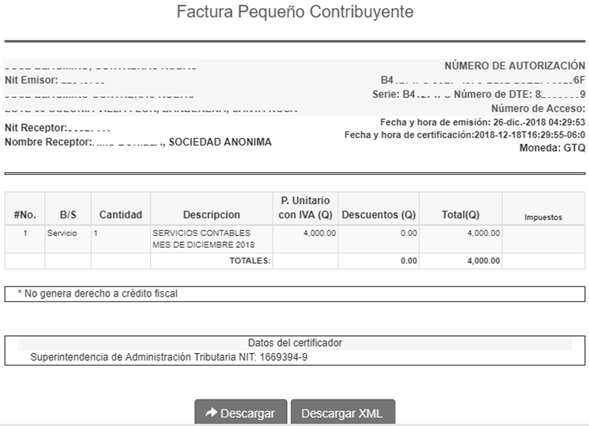
\includegraphics[width=0.8\textwidth]{imagenes/image2.png}
    
    \vspace{0.2cm}
    \raggedright \small \textbf{Nota.} \textit{Figura obtenida de \url{https://preguntas.diamantecontador.com}}
\end{figure}

En la figura 1 podemos apreciar una factura por medio del portal SAT este documento de respaldo es admitido en la Empresa, para hacer validación de Facturas de Proveedores, Facturas para viáticos y Facturas para liquidación de caja chica.

En el caso de la caja chica, se entrega primeramente un vale de caja chica, para poder desembolsar el efectivo y luego la persona que recibió el efectivo, deberá entregar un documento de respaldo como lo es la Factura contable, que debe tener el mismo monto del vale o bien debe reembolsar la diferencia entre el gasto y el efectivo entregado.

\begin{figure}[h]
    \caption{Ejemplo de Vale de Caja chica}
    \vspace{0.2cm}
    \centering
    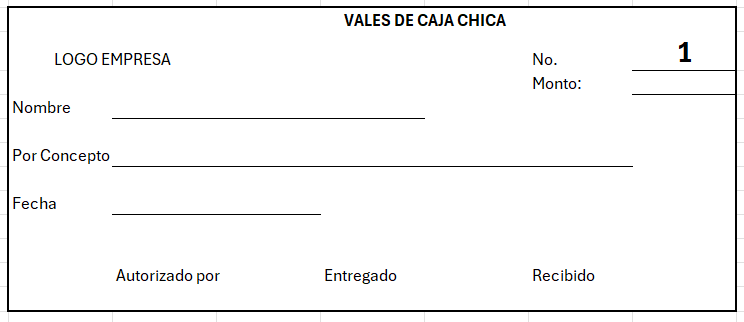
\includegraphics[width=0.8\textwidth]{imagenes/image3.png}
\end{figure}

\begin{figure}[h]
    \caption{Ejemplo de Cheque}
    \vspace{0.2cm}
    \centering
    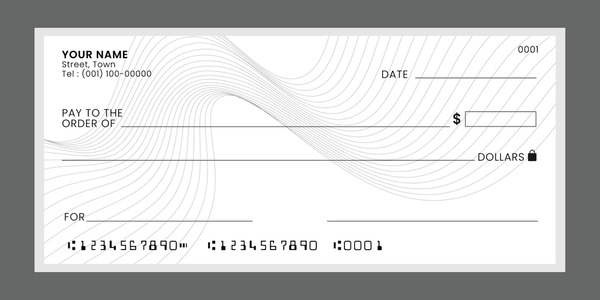
\includegraphics[width=0.8\textwidth]{imagenes/image4.jpeg}
    
    \vspace{0.2cm}
    \raggedright \small \textbf{Nota.} \textit{Figura obtenida de: \url{https://www.shutterstock.com/es/search/chequed}}
\end{figure}

\subsubsection{Gestión de Operaciones de Tesorería y Ciclo de Pagos}

Una Empresa se puede clasificar como buena organización por la forma en como administra sus ingresos y egresos monetarios. En el caso de la empresa en donde vamos a desplegar el sistema propuesto se enfoca en cuatro pilares principales los cuales gestionan el manejo monetario, que requiere de un riguroso control para evitar fugas de capital y errores administrativos.

\textbf{Fondo Fijo de Caja Chica.} Se refiere al fondo disponible que tiene la empresa para cubrir gastos menores, que normalmente no requieren de transferencias o cheques, El manejo de la caja chica es por medio de efectivo.

"El fondo de caja chica es una cantidad fija de efectivo que se utiliza para pagar gastos de pequeña cuantía. El sistema de control requiere que cada pago esté respaldado por un comprobante pre-numerado" (Horngren et al., 2012, p. 248).

Su sistema o control consta de la realización de un vale de caja chica que funge como un documento de respaldo, indicando que se realizó un desembolso de efectivo, pero este documento es provisional. El documento de respaldo de mayor interés corresponde a la factura o recibo que hace constar que se realizo el gasto del efectivo. También hay que tomar en cuenta que no siempre se gasta el efectivo indicado dentro del vale, por lo que es necesario colocar dentro de las observaciones del vale que, al momento de realizar el gasto, este fue menor al previsto, y se debe reintegrar la diferencia del gasto hacia caja chica, por ello se indica que el vale de caja chica solamente es provisional.

El sistema propuesto, permitirá el registro digital de estos comprobantes, facilitando el arqueo de caja chica y la solicitud de reintegro al contador de forma inmediata. Esto se refiere al momento de agotar el efectivo disponible.

\textbf{Gestión de Viáticos y Gastos de Viaje.} Los viáticos comprenden a la asignación de fondo para gastos de lo que los empleados tienen como beneficios. Normalmente los viáticos sirven para cubrir gastos como lo son: Gasolina, Alimentación, Hospedaje, Depreciación (Se refiere a servicio de vehículo o reparación de este).

"Los gastos de viaje deben ser estrictamente controlados mediante informes de gastos que detallen el propósito del viaje y estén acompañados por las facturas originales de soporte" (Estupiñán Gaitán, 2015, p. 55). Este Fondo debe ser fijo y al momento de ser entregados los gastos por viáticos, el empleado no debe exceder el gasto del fondo, es decir, por ejemplo, si al momento de la contratación tiene un desembolso de Q500.00 los cuales corresponden para gastos de alimentos durante 1 semana de viaje, al momento de que el empleado entregue al contador los documentos de respaldo (Facturas), estos deben sumar Q500.00 o un monto menor a ello. Esto es debido a que el contador al momento de realizar el reintegro de estos gastos lo hará al monto del fondo en su caso y si de casualidad si es de monto menor, este se realizara al monto entregado.

En el sistema propuesto, la liquidación de viáticos dejara de ser un proceso en papel o en Excel, dejando también de ser un proceso de calculo manual a realizarse de manera automática, registrando las facturas que la personal entrega. El contador realiza los reintegros generando hojas de Excel por cada reintegro y de manera manual realiza los cálculos. En el sistema propuesto, el contador registrara las facturas únicamente y el sistema generara las partidas automáticamente para que el contador únicamente realice los reintegros correspondientes.

\textbf{Cheques y Títulos de Crédito.} El cheque es un documento mercantil por el que una persona puede realizar transferencias o pagos monetarios hacia otra persona, esto se realiza mediante una entidad bancaria que funciona como intermediario entre la persona A hacia la persona B.

"El control del efectivo requiere que todos los desembolsos importantes se realicen mediante cheque, lo cual proporciona un registro permanente de cada pago" (Meigs et al., 2000, p. 160). Es decir que, a diferencia de la caja chica, los cheques pueden desembolsar cantidades grandes de dinero, son usualmente utilizado para realizar pagos a proveedores o realizar compras de grandes magnitudes. Los cheques también funcionan como documento de respaldo, ya que deja un registro de cuando y cuanto se desembolsó el recurso monetario y también a quien se realizó dicho desembolso.

La empresa lo toma de la parte de recepción de dichos cheques, al ser posfechados, estos tienen indicada una fecha de depósito y son recibidos por el contador quien se debe encargar de depositarlos correctamente en la fecha indicada del cheque, pero en el caso de tener la fecha de depósito en algún día de descanso, es recomendable realizarlo al siguiente día laboral. Este tipo de control es realizado de forma manual por medio de calendarios físicos, careciendo de alertas, por ello el sistema propuesto, promueve el uso de alertas que dan aviso el día correspondiente de depósito y también deja un registro de estos cheques para consultas futuras.

\textbf{Pago a Proveedores y Crédito Comercial.} También conocida como cuenta por pagar. Esta función corresponde a la gestión y control de pagos a proveedores los cuales normalmente contienen días Crédito (lapso que da el proveedor para poder pagar su factura), estos pagos pueden ser por compras de suministros, pago de importaciones, pago por servicios (agua, luz, teléfono etc.), entre otros rublos.

"Las cuentas por pagar representan pasivos a corto plazo que deben gestionarse para aprovechar descuentos por pronto pago y mantener relaciones sólidas con los proveedores" (Guajardo Cantú, 2014, p. 340). Estos beneficios son establecidos al momento de crear la relación empresarial por medio de un contrato entre ambas empresas.

El sistema propuesto automatizara el cálculo de vencimiento de las facturas, así como la generación de partidas de diario, para facilitar la tarea del contador. Esta función también esta involucrada el sistema de alertas que notificaran al contador el día en que debe ser efectivo el pago, junto a la partida de diario para el registro en el software que tiene actualmente la empresa.

\textbf{Nomenclatura y Catálogo de Cuentas.} Corresponde al uso de códigos y nombres para las cuentas contables, para el registro de los gastos e ingresos de manera contable para poder ser presentados en un Libro mayor.

"Un catálogo de cuentas es una lista de los nombres de todas las cuentas que aparecen en el libro mayor; permite que diferentes personas registren las transacciones de manera consistente" (Horngren et al., 2012, p. 55). Es decir que empleados como el auditor y el colaborador puedan gestionar estos registros, utilizando una misma terminología y uso de códigos, Cada empresa tiene una nomenclatura interna o bien pueden utilizar la nomenclatura bancaria, La cual es especifica y rigurosa donde se debe interactuar con cuentas de activo líquido.

\textbf{\textit{Importancia.}} Permite identificar rápidamente el origen de los fondos, por ejemplo, si un deposito fue realizado en el banco A, pero un pago fue realizado desde el banco B.

\textbf{\textit{Estructura.}} Generalmente se utiliza un sistema decimal, por ejemplo, 100101 Banco A, 100102 Banco B.

\textbf{Partidas de Diario.} La partida de diario es el registro formal de una transacción financiera. Según Guajardo Cantú (2014, p. 78), "el diario general es el libro donde se registran cronológicamente todas las operaciones de una entidad, identificando las cuentas deudoras y acreedoras". Estas partidas se manejan por medio de la Nomenclatura ya que tienen identificadas las cuentas a realizar. Cada partida representa una transacción (ventas, compras, pagos) y utilizan el sistema de partidas dobles, que básicamente es garantizar que los débitos (debe) igualen a los créditos (Haber).

El modo es como se manejan las partidas es por el medio de registros diarios o por periodos mensuales, Todo cargo tiene un abono equivalente, es decir que, por si ejemplo, tenemos un gasto de Q100.00, este gasto saldrá de una cuenta llamada Banco y se debe abonar por medio de la factura del gasto que debe tener el mismo monto. Pero esta factura se desglosa dependiendo de la cuenta contable y si contiene algún impuesto aplicable como el que es el iv. Retomando el ejemplo anterior, podemos indicar que el gasto es por viáticos y este gasto contiene IVA, entonces debemos hacer el calculo del IVA el cual es el monto de la factura dividido por 1.12 y multiplicado por .12. Véase la figura 4

\begin{figure}[h]
    \caption{Ejemplo de partida contable}
    \vspace{0.2cm}
    \centering
    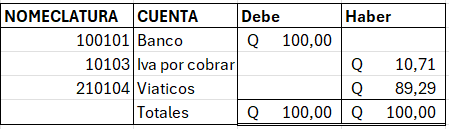
\includegraphics[width=0.8\textwidth]{imagenes/image5.png}
    
    \vspace{0.2cm}
    \raggedright \small \textbf{Nota.} \textit{Tomar en cuenta que las partidas contables contienen su número en la nomenclatura y su nombre.}
\end{figure}

El sistema propuesto desea realizar estas partidas contables de tal manera que el contador, solo ingrese los datos de la factura e indique si contiene algún impuesto, para que estas cuentas se puedan clasifiquen y realicen los cálculos correspondientes de forma automática.

\subsubsection{Optimización de Procesos mediante Alertas y Notificaciones}

La implementación de un sistema de alertas no es solo una funcionalidad técnica, sino una estrategia de control preventivo. Según Estupiñán Gaitán (2015, p. 88), las actividades de control deben incluir mecanismos que aseguren el cumplimiento de las normas y políticas establecidas por la gerencia. En un entorno donde se manejan múltiples obligaciones financieras, la notificación proactiva sustituye a la revisión reactiva, reduciendo drásticamente el margen de error humano.

\textbf{Mitigación del Riesgo de Extemporaneidad.} Uno de los problemas identificados en la empresa, es el retraso en el pago a proveedores debido a fallas en el seguimiento manual. Las alertas automatizadas permiten cumplir con el objetivo contable de "proyectar flujos de caja" y anticipar las salidas de efectivo. Al parametrizar los días de crédito (por ejemplo, 45 días), el sistema garantiza que la administración tenga visibilidad del compromiso antes de que este se convierta en una mora.

\textbf{Gestión de Excepciones y Días Inhábiles.} La lógica del sistema propuesto aborda una debilidad del control manual: la consideración de feriados y fines de semana. En Guatemala, el depósito de cheques posfechados o el pago de obligaciones debe ajustarse al calendario laboral para evitar protestos o recargos.

\begin{itemize}
    \item \textbf{Control de Cheques:} El sistema dará aviso el día correspondiente de depósito, dejando un registro para consultas futuras.
    \item \textbf{Ajuste Automático:} Si una fecha de depósito coincide con un día de descanso, el sistema alerta para realizarlo al siguiente día laboral.
\end{itemize}

\begin{table}[h]
    \centering
    \caption{Jerarquía de Alertas y su Impacto en el Control Interno}
    \vspace{0.2cm}
    \begin{tabular}{p{3cm} p{5cm} p{5cm}}
        \toprule
        \textbf{Tipo de Alerta} & \textbf{Evento Disparador} & \textbf{Objetivo de Control} \\
        \midrule
        Preventiva & 1 día antes del vencimiento de factura. & Asegurar liquidez y solvencia. \\
        Informativa & Registro exitoso de viáticos por colaborador. & Comunicación fluida Contador-Admin. \\
        Crítica & Fecha de depósito de cheque posfechado. & Proteger activos y evitar pérdidas. \\
        Cumplimiento & Límite de gasto en fondo de caja chica. & Promover eficiencia operativa. \\
        \bottomrule
    \end{tabular}
\end{table}

\subsubsection{Sistemas de Información Contable (SIC) y Transformación Digital}

Corresponde al ecosistema donde vivirá el software. Un SIC no es solo una base de datos; es una estructura que combina recursos humanos, tecnológicos y registros para producir información útil.

"Un sistema de información contable recolecta, procesa y comunica información financiera sobre una entidad económica a una amplia variedad de personas" (Meigs et al., 2000, p. 8).

Para la empresa en la cual se desplegará el sistema propuesto, esto representaría la evolución del sistema manual a uno automatizado. Según Estupiñán Gaitán (2015, p. 88),'' la automatización elimina los "cuellos de botella" que se forman cuando la información depende de procesos humanos repetitivos, como la transcripción de datos de facturas a hojas de cálculo''. El contador dejara de utilizar documentos en papel, así como hojas de Excel para realizar todo automatizado por medio del sistema propuesto.

\subsubsection{El Concepto de Computación en la Nube y Repositorios Digitales}

Representan la evolución moderna del almacenamiento y la gestión de la información, por medio de estructuras virtuales que se manejan en torno a la Red de internet, permitiendo así a las organizaciones y/o usuarios poder acceder a esta desde cualquier parte, solamente se necesita algún dispositivo electrónico inteligente, como: Teléfonos móviles, Computadoras. También permite que el almacenamiento crezca conforme la empresa lo requiera, por lo que, la empresa tiene control sobre el mismo.

\subsubsection{Seguridad de la Información y Perfiles de Usuario}

Las organizaciones evalúan riesgos y por medio de este análisis aplican medidas de seguridad de datos tanto para el personal como para la empresa, en el cumplimiento de datos personales. Lo primordial es utilizar contraseñas las cuales deben ser complejas y únicas. Para ello sirve la seguridad de la información, para proteger datos confidenciales mediante políticas y herramientas que garantizan la confidencialidad, integridad y disponibilidad.

Se crean perfiles de usuario, los cuales deben ser por niveles de autoridad, Teniendo como el nivel mas alto. A la persona que puede modificar y administrar la mayoría del software. Esta función mayormente es utilizada para poder limitar el acceso no autorizado y prevención de fugas de información.

"Las actividades de control incluyen verificaciones independientes y la documentación adecuada para asegurar un control efectivo" (Horngren et al., 2012, p. 240). En el sistema propuesto, esto se traduce en la autenticación y Autorización. Definiendo roles con niveles de acceso para poder proteger la información mediante contraseñas y que solo las personas con accesos puedan tener control en ella, algo que en los documentos de Excel no puede garantizar.

\subsection{Marco Tecnológico}

Se hablará sobre las herramientas, lenguajes de programación y metodologías de ingeniería de software que servirán como base para la construcción del sistema propuesto. La sección de estas tecnologías responde a los criterios de seguridad, estabilidad y eficiencia exigidos por el control interno de la empresa don se desplegará el sistema propuesto.

\subsubsection{Metodología de Desarrollo: Proceso Unificado Racional (RUP)}

Se opta por el uso de esta metodología por ser un framework, para el desarrollo de software, estructurado e iterativo, creado por Rational Software (ahora es parte de IBM). Según Sommerville (2011, p. 30), RUP es un modelo de proceso moderno que se caracteriza por ser iterativo e incremental, lo que permite reducir riesgos desde las etapas tempranas del proyecto.

A diferencia de un proceso lineal donde no se ve el resultado hasta el final, RUP permite crear "versiones" pequeñas y funcionales. "El desarrollo iterativo permite que el equipo de desarrollo aprenda de las versiones anteriores y refine los requisitos del usuario" (Sommerville, 2011, p. 30). y organiza el trabajo en cuatro fases criticas:

\textbf{Inicio (Inception).} Se define el alcance del proyecto, visión y se identifican los riesgos principales. Por ejemplo, definimos como un posible riesgo la transición de archivos de Excel a una base de datos centralizada.

\textbf{Elaboración (Elaboration).} Diseña la arquitectura, refina requisitos y mitiga riesgos. Siguiendo el ejemplo anterior, podemos crear las bases de datos para que estas se adapten a la información del Excel.

\textbf{Construcción (Construction)}. Es la fase de programación y diseño de los módulos, también acá se realizan pruebas. Por ejemplo, creamos módulos por cada tipo de función que deseamos como lo podría ser, (Viáticos, Cheques, Caja Chica).

\textbf{Transición (Transition).} El sistema se entrega a los usuarios finales (Contador y Administrador) para pruebas y despliegue. Se realizan capacitaciones para dar a conocer el producto final y resolución de dudas, acá es donde ya se instala el sistema.

"RUP se basa en el uso de casos de uso para guiar el desarrollo y se centra en la arquitectura, lo que garantiza que el sistema sea robusto antes de añadir grandes cantidades de código" (Larman, 2004, p. 25). Casos de Uso: en esencia es como el usuario interactúa con el sistema, el usuario desea realizar una acción como lo es registrar una factura, entonces le debe dar esa indicación al sistema, ingresando los datos de la factura y luego el sistema debe llegar a su objetivo, por ejemplo, el registro de la factura.

\begin{figure}[h]
    \caption{Ejemplo de caso de Uso}
    \vspace{0.2cm}
    \centering
    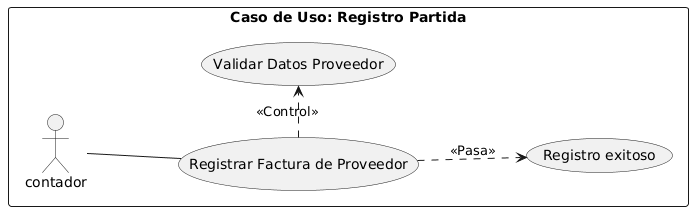
\includegraphics[width=0.8\textwidth]{imagenes/image6.png}
\end{figure}

El ejemplo de la figura 5 demuestra como el contador registra la factura del proveedor, luego el sistema valida los datos del proveedor, para su control y después pasa a su objetivo el cual es el registro exitoso.

\subsubsection{Lenguajes y Herramientas}

\textbf{Angular.} Es la cara del sistema (Frontend). Es decir que es lo que el usuario ve y con lo que interactúa en su pantalla. Angular es un marco de trabajo (framework), el cual fue desarrollado por Google que permite que una página Web tenga la misma sensación como lo es utilizar aplicaciones de escritorio, de manera rápida y fluida.

"Los marcos de trabajo como Angular permiten que el desarrollador se concentre en la experiencia del usuario, automatizando tareas repetitivas de actualización de la pantalla" (Freeman, 2020, p. 45).

"Angular es una plataforma de desarrollo, construida sobre TypeScript. Como plataforma, Angular incluye un marco de trabajo basado en componentes para construir aplicaciones web escalables y una colección de bibliotecas bien integradas que cubren diversas funciones como el enrutamiento y la gestión de formularios" (Google, 2024a, párr. 2).

Esto significa que Angular actúa como un "kit de construcción" profesional que ya tiene todas las piezas seguras para crear modulos se adaptan a cualquier pantalla de computadora.

Esto en el sistema propuesto corresponde a todo el apartado visual e interactivo que vera el usuario.

\textbf{Python.} Es la parte invisible para el usuario (Backend). Es el lenguaje de programación que utilizaremos para la construcción de la lógica de todo el sistema propuesto, desde operaciones básicas, como la automatización de partidas de diario. Se podría decir que es el cerebro de todo el sistema.

"Python destaca por su capacidad para manejar lógica de negocio compleja y su facilidad para integrarse con otros sistemas" (Van Rossum, 2018).

"Python es un lenguaje de programación interpretado, orientado a objetos y de alto nivel con semántica dinámica. Sus estructuras de datos integradas, combinadas con el tipado y el enlace dinámicos, lo hacen muy atractivo para el desarrollo rápido de aplicaciones" (Python Software Foundation, 2024, párr. 1).

En términos sencillos esto significa que Python permite escribir las reglas de negocio (como el cálculo de impuestos guatemaltecos o alertas de cheques) de forma clara y segura, facilitando que el sistema sea fácil de mantener y actualizar en el futuro.

Se opta por Python por su gran versatilidad, por lo que se permite usarse en casi cualquier campo tecnológico. Su sintaxis es sencilla, contiene una amplia selección de librerías, su comunidad es inmensa y no utiliza tantas líneas de código como otros lenguajes de programación.

\textbf{PostgreSQL}, Es una base de datos gratuita y potente, Usa el lenguaje de SQL y esta preparado para maneja de forma segura la información.Al ser de codigo abierto tiene tuna gran comunidad de programadores en todo el mundo, por lo que se mantiene actualizada y con mejoras constantes.

"PostgreSQL incluye numerosas funciones diseñadas para ayudar a los desarrolladores a crear aplicaciones, a los administradores a proteger la integridad de los datos y crear entornos tolerantes a fallos, y a gestionar sus datos independientemente de su tamaño. Además de ser gratuito y de código abierto , PostgreSQL es altamente extensible. Por ejemplo, puede definir sus propios tipos de datos, crear funciones personalizadas e incluso escribir código en diferentes lenguajes de programación sin necesidad de recompilar la base de datos" (PostgreSQL Global Development Group, s. f., párr. 1).

\textbf{Token JWT}. Sirve como metodo de seguridad que al momento de que un usuario desea ingresar debe verificar si este existe en la base de datos PostgreSQL, a partir de ello pasa por el backend quien valida que tipo de accesos tiene y estos se muestran en el Angular al abrir el navegador

Si el contador registra un cheque desde su oficina, el administrador verá la actualización en su pantalla instantáneamente sin necesidad de refrescar la página o enviar archivos por correo electrónico.

"PostgreSQL admite varios métodos de autenticación de clientes. Cuando un cliente se conecta al servidor de base de datos, especifica con qué nombre de usuario de base de datos desea conectarse. Luego, el servidor determina si acepta la conexión en función del método de autenticación configurado para ese cliente y usuario." (PostgreSQL Global Development Group, 2024, cap. 21).

"El módulo pgcrypto proporciona funciones criptográficas para PostgreSQL. Incluye funciones para el almacenamiento con resumen cifrado de contraseñas (hashing), cifrado de clave simétrica y cifrado de clave pública."(PostgreSQL Global Development Group, 2024, apendice F).

\begin{table}[htbp]
    \centering
    \caption{Analogía y Comparación entre el Sistema Actual y el Propuesto}
    \label{tab:comparativa_sistema}
    \vspace{0.2cm}
    \begin{tabular}{p{3cm} p{5.5cm} p{6.5cm}}
        \toprule
        \textbf{Concepto} & \textbf{Sistema Actual (Manual/Excel)} & \textbf{Sistema Propuesto (Web)} \\
        \midrule
        \textbf{Almacenamiento} & Archivos en disco duro local u hojas de cálculo aisladas. & Base de datos relacional PostgreSQL con acceso centralizado. \\
        \addlinespace
        \textbf{Seguridad} & Sin restricciones o archivos protegidos con clave simple; cualquiera puede editar. & Autenticación por tokens (JWT), control de roles y permisos por usuario. \\
        \addlinespace
        \textbf{Cálculos e Integridad} & Fórmulas en Excel susceptibles a borrado o modificación accidental. & Lógica de negocio automatizada en Python con validación en Angular. \\
        \addlinespace
        \textbf{Respaldos} & Copias manuales esporádicas en memorias USB o correos electrónicos. & Respaldos automatizados (\textit{backups}) e integridad transaccional ACID. \\
        \bottomrule
    \end{tabular}
\end{table}
\setcounter{section}{2} % Fuerza a LaTeX a iniciar la numeración en la Sección 3

\section{Capítulo III - Marco Metodológico}

En este capitulo se explica por qué se decide utilizar la metodología de ingeniería de software basada en el Proceso Unificado de Rational (RUP, por sus siglas en inglés), la cual rige las fases de análisis, diseño, desarrollo e implementación del proyecto. Se proporciona una descripción clara y estructurada del proceso de tal manera que se cumpla con el propósito de garantizar la transparencia, el rigor técnico, la trazabilidad de los requerimientos y la calidad integral de la plataforma web propuesta.

El desarrollo del sistema propuesto se basara en el análisis y diseño del modelo de  base  de datos la cual sera relacional en PostgreSQL, de esta manera se aseguran las operaciones contables, se fortalece la seguridad de los datos, y es una excelente herramienta para los módulos que se desean los cuales son la autenticación de usuarios, la gestión de cheques postfechados, el control de caja chica, liquidación de viáticos, control de pagos a proveedores y un sistema de alertas. También se aborda la revisión y optimización de los flujos de trabajo actuales para disminuir las redundancias, la preparación de reglas de cálculo contable para la futura integración con un backend, la implementación del apartado visual del frontend en Angular con TypeScript y el establecimiento de protocolos para el mantenimiento correctivo y adaptativo del software.

\subsection{Antecedentes} 

En la distribuida farmacéutica, los procesos de gestión administrativa y financiera diaria correspondientes al control de deposito de cheques postfechados, la creación de cheques de caja chica, el pago de liquidación de viáticos y el control de pagos de proveedores con crédito, actualmente se realizan mediante cálculos manuales y libros de calculo con Microsoft Excel.

Al realizar los procesos de esta manera, han generado inconvenientes en la gestión de la empresa, los cuales destacan la desorganización de fechas para pago a proveedores, como el deposito de cheques, no se realizan a tiempo. Otro de los inconvenientes generados es dentro de los cálculos contables, al ser estos manuales a menudo se colocan mal las formulas en las hojas de Excel o bien existen borrados accidentales. A raíz de ello surge la necesidad de desarrollar e implementar una aplicación web centralizada con frontend Angular, backend desarrollado en Python y base de datos relacional PostgreSQL, reduciendo así estos errores de calculo y asegurando por medio de las alertas, que todo se deposite/pague en la fecha correcta, remplazando de esta manera el uso de procesos manuales, asegurando la integridad, confidencialidad y disponibilidad de la información financiera.

\subsection{Impacto}

La implementación del sistema propuesto genera un impacto innovador en 3 áreas fundamentales dentro de la empresa, siendo estas: operativa, financiera y de seguridad digital

\paragraph{Operativa}. Se planea automatizar los cálculos contables, la creación de partidas de diario automáticamente, se pretende eliminar la duplicidad en los registros de datos y reducción del tiempo que le toma al contador realizar estas tareas rutinarias.

\paragraph{Financiera}. Se soluciona los atrasos en depósitos y/o pagos, por medio de las alertas automáticas, las cuales notifican con anticipación sobre las fechas cercanas, también se pretende un correcto registro respecto a las facturas que los proveedores generan a la empresa. Se descargaran estas facturas directamente de la SAT, se subirá esta información al sistema y esta las registrara y clasificara automáticamente.

\paragraph{Seguridad Digital}.En cuanto a la seguridad e integridad de la información, la aplicación reemplaza el uso de archivos locales vulnerables por una base de datos relacional PostgreSQL con autenticación basada en roles y tokens JWT, garantizando la trazabilidad completa de cada movimiento contable.

\subsection{Beneficios}

La implementación del sistema propuesto brinda un conjunto de herramientas y ventajas, escalables y competitivas para la empresa. Siendo la primordial en la centralización de la información financiera diaria, por medio de la arquitectura de la base de datos relacional.

Destaca también la seguridad en el registro de la información, ya que el contador no se dedicaría a tabular todas las facturas que recibe la empresa. Ahora, él descargará toda la información que proporciona la SAT, esta información la sube como un formato de Excel al sistema propuesto, que se encarga de la clasificación automática de los proveedores con crédito para pago. Las facturas que se estiman correspondan a viáticos. De esta manera el contador ya no escribe casi nada, ahora se encarga de monitoriar la información y realizar las modificaciones si corresponde.

Estos procesos automáticos beneficiarían tanto al contador como al administrador, reduciendo esfuerzo y tiempo, ya ahora como ya existe una base de datos concreta, ya se pueden generar reportes correspondientes a estos datos. Con el tema de los cheques postfechados, el contador aun tendría que typear esta información, pero ya el sistema se encargaría de clasificar la fecha correspondiente del deposito, calculando los feriados y/o descansos de fin de semana.


\subsection{Referencias}

Las referencias operativas representan el conjunto de documentos base, instrumentos de registro, formularios físicos y archivos digitales que la distribuidora farmacéutica utiliza de manera cotidiana para normar y llevar el control de sus transacciones financieras. Dentro del marco de la metodología del Proceso Unificado de Rational (RUP), estos artefactos constituyen la línea base del negocio (Business Baseline), ya que permiten a los analistas de sistemas comprender la estructura de los datos actuales, identificar los flujos de información manuales e inferir las reglas de negocio necesarias para el diseño de los nuevos módulos del sistema.

El análisis de estos documentos de base resulta indispensable para asegurar que el software capture la totalidad de las variables operativas requeridas por el área contable. La Tabla 2 detalla los instrumentos de control primarios identificados en la empresa, los cuales sirvieron como insumo técnico directo para el levantamiento de requerimientos funcionales y la posterior estructuración de las tablas del modelo relacional en PostgreSQL.

{
\small
\setstretch{1.15}
\setlength{\parindent}{0pt}
\begin{xltabular}{\linewidth}{
    >{\raggedright\arraybackslash}p{2.8cm} 
    >{\raggedright\arraybackslash}p{3.2cm} 
    >{\raggedright\arraybackslash}X 
    >{\raggedright\arraybackslash}p{2.0cm}
}

    % --- Encabezado de la primera página ---
    \caption{Documentos de Control de Registros de Movimientos} \label{tab:referencias_operativas} \\
    \toprule
    \textbf{Tipo de Referencia} & \textbf{Referencia} & \textbf{Descripción} & \textbf{Fecha} \\
    \midrule
    \endfirsthead


    \toprule
    \textbf{Tipo de Referencia} & \textbf{Referencia} & \textbf{Descripción} & \textbf{Fecha} \\
    \midrule
    \endhead

    % --- Cierre al final de las páginas intermedias ---
    \bottomrule
    \endfoot

    % --- Cierre final de la tabla ---
    \bottomrule
    \endlastfoot

    % --- Filas de datos ---
    Hoja de cálculo & Cheques Postfechados & Documento donde se llevan los registros de los cheques para ser depositados en fechas específicas. & 03/04/2026 \\
    \addlinespace
    Hoja de cálculo & Liquidación de Viáticos & Documento donde se lleva el control de los reintegros a realizar a los colaboradores, conforme a la programación. & 05/05/2026 \\
    \addlinespace
    Hoja de cálculo & Control de Caja Chica & Documento donde se registran las facturas y se calculan los ingresos y egresos de caja chica. & 05/05/2026 \\
    \addlinespace
    Hoja de cálculo & Facturas de Proveedores & Documento que sirve para registrar las facturas de los proveedores a pagar con días de crédito, creación de partida de diario y fecha para el pago. & 01/05/2026 \\
    \addlinespace
    Calendario & Programaciones & Calendario digital del equipo donde se anotan las programaciones de pagos, depósito de cheques y días para pago de viáticos. & 01/05/2026 \\
    \addlinespace
    Cuaderno & Cuaderno Auxiliar & Cuaderno físico que sirve como auxiliar para anotaciones de cálculos y recordatorios para pagos y depósitos. & 01/05/2026 \\

\end{xltabular}
}
\subsection{Descripción del Problema}

En la empresa, la gestión diaria de las operaciones contables, como el control de cheques postfechados, el manejo de caja chica la liquidación de los colaboradores y la programación de pagos, no están implementadas dentro del software actual, por lo que se opta por utilizar procesos manuales como lo son Hojas de calculo en libros de Excel, cuaderno de anotaciones y calendarios físicos o virtuales. De esta manera se han generado retrasos, errores humanos de cálculos y dificultad en el seguimiento de fechas. 

Al no tener estos servicios dentro del software actual, la información se encuentra dispersa entre archivos de Excel, anotaciones de cuadernos y recordatorios en calendarios, sin alertas.


{
\small
\setstretch{1.15}
\setlength{\parindent}{0pt}
\begin{xltabular}{\linewidth}{
    >{\raggedright\arraybackslash}p{4.2cm} 
    >{\raggedright\arraybackslash}X
}

    % --- Encabezado principal (Primera página) ---
    \caption{Descripción del Problema y Propuesta de Solución} \label{tab:descripcion_problema} \\
    \toprule
    \textbf{Criterio / Pregunta} & \textbf{Descripción Operativa} \\
    \midrule
    \endfirsthead

    % --- Encabezado de continuación (Si la tabla se divide entre páginas) ---
    \toprule
    \textbf{Criterio / Pregunta} & \textbf{Descripción Operativa} \\
    \midrule
    \endhead

    % --- Cierre en la página intermedia ---
    \bottomrule
    \endfoot

    % --- Cierre final de la tabla ---
    \bottomrule
    \endlastfoot

    % --- Filas de contenido ---
    \textquestiondown Cuál es el problema? & Ineficiencia y falta de control en la gestión de cheques postfechados, caja chica, viáticos y facturas de proveedores debido al uso de registros en papel y hojas de cálculo manuales. \\
    \addlinespace
    \textquestiondown A quiénes afecta? & Al departamento de contabilidad, auditoría interna y administración de la distribuidora farmacéutica. \\
    \addlinespace
    \textquestiondown Por qué ocurre? & Porque el software principal no contiene estas funciones, ya que está más enfocado en recursos de mayor escala como libro diario, balance general, etc. \\
    \addlinespace
    \textquestiondown Cuál es la solución propuesta? & Implementar una aplicación web centralizada que por medio de un archivo de excel descargado directamente de la SAT,automatice la clasificación de facturas y la preparación de partidas y realice cálculos, partidas de diario y genere alertas automáticas para aumentar la eficiencia y disminuir retrasos. \\

\end{xltabular}
}

\subsection{Funcionalidades Requeridas}

Se detallan los requerimientos funcionales del sistema, registrando su numero de requerimiento  (Id), su clasificación prioritaria entre otros aspectos que debe satisfacer el sistema propuesto, dentro del marco de la metodología RUP.

{
\small
\setstretch{1.15}
\setlength{\parindent}{0pt}
\begin{xltabular}{\linewidth}{
    >{\raggedright\arraybackslash}p{4.2cm} 
    >{\raggedright\arraybackslash}X
}

    % --- Encabezado Principal (APA 7) ---
    \caption{Requerimiento Funcional: Autenticación y Control de Acceso (Login)} \label{tab:req001} \\
    \toprule
    \textbf{Id. Requerimiento:} REQ001 & \textbf{Clasificación o prioridad:} Alta \\
    \textbf{Nombre Requerimiento:} & Login y Autenticación de Usuarios \\
    \midrule
    \textbf{No. Func.} & \textbf{Funcionalidad} \\
    \midrule
    \endfirsthead

    % --- Encabezado en Siguiente Página ---
    \toprule
    \textbf{Id. Requerimiento:} REQ001 & \textbf{Clasificación o prioridad:} Alta \\
    \textbf{Nombre Requerimiento:} & Login y Autenticación de Usuarios \\
    \midrule
    \textbf{No. Func.} & \textbf{Funcionalidad} \\
    \midrule
    \endhead

    % --- Cierres de Tabla ---
    \bottomrule
    \endfoot

    \bottomrule
    \endlastfoot

    % --- Filas de Contenido ---
    001 & Permitirá el acceso a los usuarios autorizados del sistema. \\
    \addlinespace
    002 & Permitirá el registro de usuarios nuevos por medio del administrador del sistema. \\
    \addlinespace
    003 & Permitirá ingresar la contraseña del usuario, la cual será procesada y protegida de forma segura. \\
    \addlinespace
    004 & Se verificará el usuario, contraseña y estado activo en la base de datos PostgreSQL emitiendo un token de acceso. \\
    \addlinespace
    005 & En caso de error en las credenciales, se mostrará un mensaje de advertencia y se restablecerán los campos para intentar de nuevo. \\

\end{xltabular}
}

{
\small
\setstretch{1.15}
\setlength{\parindent}{0pt}
\begin{xltabular}{\linewidth}{
    >{\raggedright\arraybackslash}p{4.2cm} 
    >{\raggedright\arraybackslash}X
}

    % --- Encabezado Principal (APA 7) ---
    \caption{Requerimiento Funcional: Importación y Procesamiento de Reportes SAT} \label{tab:req002_sat} \\
    \toprule
    \textbf{Id. Requerimiento:} REQ002 & \textbf{Clasificación o prioridad:} Alta \\
    \textbf{Nombre Requerimiento:} & Módulo de Carga e Importación de Facturas SAT \\
    \midrule
    \textbf{No. Func.} & \textbf{Funcionalidad} \\
    \midrule
    \endfirsthead

    % --- Encabezado en Siguiente Página ---
    \toprule
    \textbf{Id. Requerimiento:} REQ002 & \textbf{Clasificación o prioridad:} Alta \\
    \textbf{Nombre Requerimiento:} & Módulo de Carga e Importación de Facturas SAT \\
    \midrule
    \textbf{No. Func.} & \textbf{Funcionalidad} \\
    \midrule
    \endhead

    % --- Cierres de Tabla ---
    \bottomrule
    \endfoot

    \bottomrule
    \endlastfoot

    % --- Filas de Contenido ---
    001 & Permitirá la carga masiva del archivo de Excel con el reporte mensual de facturas emitidas y recibidas desde la plataforma de la SAT. \\
    \addlinespace
    002 & Analizará y extraerá automáticamente los campos del archivo (NIT, nombre de proveedor, número de documento, fecha, monto, impuestos etc...). \\
    \addlinespace
    003 & Tomara el numero de autorizacion de la factura como identificador lógico para prevenir el registro duplicado de facturas en la base de datos PostgreSQL. \\
    \addlinespace
    004 & Clasificará los registros importados y los redistribuirá de manera automática hacia los módulos correspondientes (Proveedores, Viáticos o Caja Chica). \\

\end{xltabular}
}

{
\small
\setstretch{1.15}
\setlength{\parindent}{0pt}
\begin{xltabular}{\linewidth}{
    >{\raggedright\arraybackslash}p{4.2cm} 
    >{\raggedright\arraybackslash}X
}

    % --- Encabezado Principal (APA 7) ---
    \caption{Requerimiento Funcional: Control de Cheques Postfechados} \label{tab:req003_cheques} \\
    \toprule
    \textbf{Id. Requerimiento:} REQ003 & \textbf{Clasificación o prioridad:} Alta \\
    \textbf{Nombre Requerimiento:} & Gestión de Cheques Postfechados \\
    \midrule
    \textbf{No. Func.} & \textbf{Funcionalidad} \\
    \midrule
    \endfirsthead

    % --- Encabezado en Siguiente Página ---
    \toprule
    \textbf{Id. Requerimiento:} REQ003 & \textbf{Clasificación o prioridad:} Alta \\
    \textbf{Nombre Requerimiento:} & Gestión de Cheques Postfechados \\
    \midrule
    \textbf{No. Func.} & \textbf{Funcionalidad} \\
    \midrule
    \endhead

    % --- Cierres de Tabla ---
    \bottomrule
    \endfoot

    \bottomrule
    \endlastfoot

    % --- Filas de Contenido ---
    001 & Permitirá registrar cheques con cliente, banco del cheque, banco de depósito, número de cheque, monto, fecha de recepción y fecha de depósito.  \\
    \addlinespace
    002 & Permitirá actualizar el estado del cheque entre Pendiente, Depositado, Anulado y Rechazado, registrando la fecha de recepción y, cuando corresponda, la recepción del rechazo. \\
    \addlinespace
    003 & Mostrará una matriz con cliente, bancos, fechas, monto, estado y una opción desplegable de Asignación con factura, visitador, días vencidos y número de recibo. \\
    \addlinespace
    004 & Utilizará el número de cheque como identificador lógico para evitar duplicados y permitirá asignar la cuenta contable correspondiente cuando sea necesario. \\
    \addlinespace
    005 & Programará el depósito en el calendario y permitirá registrar bancos, ajustar fechas hábiles y gestionar rechazos o re-depósitos. \\

\end{xltabular}
}

{
\small
\setstretch{1.15}
\setlength{\parindent}{0pt}
\begin{xltabular}{\linewidth}{
    >{\raggedright\arraybackslash}p{4.2cm} 
    >{\raggedright\arraybackslash}X
}

    % --- Encabezado Principal (APA 7) ---
    \caption{Requerimiento Funcional: Control de Caja Chica} \label{tab:req004_cajachica} \\
    \toprule
    \textbf{Id. Requerimiento:} REQ004 & \textbf{Clasificación o prioridad:} Alta \\
    \textbf{Nombre Requerimiento:} & Creación y Control de Fondo de Caja Chica \\
    \midrule
    \textbf{No. Func.} & \textbf{Funcionalidad} \\
    \midrule
    \endfirsthead

    % --- Encabezado en Siguiente Página ---
    \toprule
    \textbf{Id. Requerimiento:} REQ004 & \textbf{Clasificación o prioridad:} Alta \\
    \textbf{Nombre Requerimiento:} & Creación y Control de Fondo de Caja Chica \\
    \midrule
    \textbf{No. Func.} & \textbf{Funcionalidad} \\
    \midrule
    \endhead

    % --- Cierres de Tabla ---
    \bottomrule
    \endfoot

    \bottomrule
    \endlastfoot

    % --- Filas de Contenido ---
    001 & Permitirá llamar facturas FEL/SAT mediante el número de factura y registrar manualmente Recibos/otros documentos con nombre, descripción, fecha y monto. \\
    \addlinespace
    002 & Separará los Movimientos de la Partida contable y calculará subtotales, IVA crédito fiscal, cuentas de gasto y contrapartida bancaria. \\
    \addlinespace
    003 & Permitirá asignar una cuenta de nomenclatura a facturas no reconocidas y generará la partida con cuentas de gasto, IVA crédito y Bancos o Cuenta transitoria. \\
    \addlinespace
    004 & Generará un resumen imprimible de Caja chica con fecha, tipo de documento, número de factura, nombre, descripción y monto. \\

\end{xltabular}
}

{
\small
\setstretch{1.15}
\setlength{\parindent}{0pt}
\begin{xltabular}{\linewidth}{
    >{\raggedright\arraybackslash}p{4.2cm} 
    >{\raggedright\arraybackslash}X
}

    % --- Encabezado Principal (APA 7) ---
    \caption{Requerimiento Funcional: Liquidación y Reintegro de Viáticos} \label{tab:req005_viaticos} \\
    \toprule
    \textbf{Id. Requerimiento:} REQ005 & \textbf{Clasificación o prioridad:} Alta \\
    \textbf{Nombre Requerimiento:} & Gestión y control de Viáticos \\
    \midrule
    \textbf{No. Func.} & \textbf{Funcionalidad} \\
    \midrule
    \endfirsthead

    % --- Encabezado en Siguiente Página ---
    \toprule
    \textbf{Id. Requerimiento:} REQ005 & \textbf{Clasificación o prioridad:} Alta \\
    \textbf{Nombre Requerimiento:} & Gestión y control de Viáticos \\
    \midrule
    \textbf{No. Func.} & \textbf{Funcionalidad} \\
    \midrule
    \endhead

    % --- Cierres de Tabla ---
    \bottomrule
    \endfoot

    \bottomrule
    \endlastfoot

    % --- Filas de Contenido ---
    001 & Permitirá vincular facturas FEL/SAT al colaborador mediante el número de factura y asignar manualmente una cuenta de nomenclatura cuando el concepto no sea reconocido. \\
    \addlinespace
    002 & Permitirá registrar colaboradores con varios territorios y asignar cada gira a un territorio y a la semana 1, 2, 3, 4 o 5 cuando aplique. \\
    \addlinespace
    003 & Permitirá clasificar facturas por Viáticos, Movilidad, Actividades y Bonos/otros gastos; la Movilidad se habilitará para la primera semana del mes. \\
    \addlinespace
    004 & Generará una partida semanal con todos los gastos de la liquidación y una partida transitoria para facturas pendientes de reintegro o pago al cierre del mes. \\

\end{xltabular}
}

{
\small
\setstretch{1.15}
\setlength{\parindent}{0pt}
\begin{xltabular}{\linewidth}{
    >{\raggedright\arraybackslash}p{4.2cm} 
    >{\raggedright\arraybackslash}X
}

    % --- Encabezado Principal (APA 7) ---
    \caption{Requerimiento Funcional: Programación de Pagos a Proveedores} \label{tab:req006_proveedores} \\
    \toprule
    \textbf{Id. Requerimiento:} REQ006 & \textbf{Clasificación o prioridad:} Alta \\
    \textbf{Nombre Requerimiento:} & Programación de Pagos a Proveedores \\
    \midrule
    \textbf{No. Func.} & \textbf{Funcionalidad} \\
    \midrule
    \endfirsthead

    % --- Encabezado en Siguiente Página ---
    \toprule
    \textbf{Id. Requerimiento:} REQ006 & \textbf{Clasificación o prioridad:} Alta \\
    \textbf{Nombre Requerimiento:} & Programación de Pagos a Proveedores \\
    \midrule
    \textbf{No. Func.} & \textbf{Funcionalidad} \\
    \midrule
    \endhead

    % --- Cierres de Tabla ---
    \bottomrule
    \endfoot

    \bottomrule
    \endlastfoot

    % --- Filas de Contenido ---
    001 & Permitirá registrar proveedores por NIT, completar automáticamente el nombre comercial y de registro, indicar días de crédito, cuenta de nomenclatura, Retención IVA y Retención ISR. \\
    \addlinespace
    002 & Permitirá desplegar las facturas del proveedor por mes y mostrar número, emisión, vencimiento, retenciones, otros descuentos, estado y reprogramación. \\
    \addlinespace
    003 & Permitirá actualizar el estado de la factura entre Pendiente, Pagada y Anulada, conservando la trazabilidad de la reprogramación. \\
    \addlinespace
    004 & Permitirá generar por separado la partida dentro del mes y la partida transitoria; incluirá gastos e IVA crédito en el Debe y retenciones y descuentos como cuentas independientes en el Haber. \\


\end{xltabular}
}

{
\small
\setstretch{1.15}
\setlength{\parindent}{0pt}
\begin{xltabular}{\linewidth}{
    >{\raggedright\arraybackslash}p{4.2cm} 
    >{\raggedright\arraybackslash}X
}

    % --- Encabezado Principal (APA 7) ---
    \caption{Requerimiento Funcional: Calendario Integrado y Programación Operativa} \label{tab:req007_calendario} \\
    \toprule
    \textbf{Id. Requerimiento:} REQ007 & \textbf{Clasificación o prioridad:} Alta \\
    \textbf{Nombre Requerimiento:} & Módulo de Calendario Dinámico y Programación \\
    \midrule
    \textbf{No. Func.} & \textbf{Funcionalidad} \\
    \midrule
    \endfirsthead

    % --- Encabezado en Siguiente Página ---
    \toprule
    \textbf{Id. Requerimiento:} REQ007 & \textbf{Clasificación o prioridad:} Alta \\
    \textbf{Nombre Requerimiento:} & Módulo de Calendario Dinámico y Programación \\
    \midrule
    \textbf{No. Func.} & \textbf{Funcionalidad} \\
    \midrule
    \endhead

    % --- Cierres de Tabla ---
    \bottomrule
    \endfoot

    \bottomrule
    \endlastfoot

    % --- Filas de Contenido ---
    001 & Unificará en una vista de calendario los depósitos de cheques, vencimientos de proveedores y giras de viáticos. \\
    \addlinespace
    002 & Permitirá consultar y reprogramar actividades desde la interfaz del calendario, conservando el vínculo con el módulo de origen. \\
    \addlinespace
    003 & Ofrecerá vistas diaria, semanal y mensual con filtros visuales por módulo y tipo de compromiso. \\
    \addlinespace
    004 & Mantendrá la fecha reprogramada asociada al registro operativo para facilitar seguimiento y alertas. \\

\end{xltabular}
}

{
\small
\setstretch{1.15}
\setlength{\parindent}{0pt}
\begin{xltabular}{\linewidth}{
    >{\raggedright\arraybackslash}p{4.2cm} 
    >{\raggedright\arraybackslash}X
}

    % --- Encabezado Principal (APA 7) ---
    \caption{Requerimiento Funcional: Nomenclatura Contable y Partidas Automáticas} \label{tab:req008_nomenclatura} \\
    \toprule
    \textbf{Id. Requerimiento:} REQ008 & \textbf{Clasificación o prioridad:} media \\
    \textbf{Nombre Requerimiento:} & Nomenclatura y paridas de Diario \\
    \midrule
    \textbf{No. Func.} & \textbf{Funcionalidad} \\
    \midrule
    \endfirsthead

    % --- Encabezado en Siguiente Página ---
    \toprule
    \textbf{Id. Requerimiento:} REQ008 & \textbf{Clasificación o prioridad:} Alta \\
    \textbf{Nombre Requerimiento:} & Nomenclatura y paridas de Diario \\
    \midrule
    \textbf{No. Func.} & \textbf{Funcionalidad} \\
    \midrule
    \endhead

    % --- Cierres de Tabla ---
    \bottomrule
    \endfoot

    \bottomrule
    \endlastfoot

    % --- Filas de Contenido ---
    001 & Permitirá registrar cuentas mediante código, nombre y naturaleza Debe o Haber, además de consultar y actualizar su estado. \\
    \addlinespace
    002 & Permitirá seleccionar las cuentas de nomenclatura para clasificar facturas y construir partidas con cuentas independientes. \\
    \addlinespace
    003 & Permitirá asociar una cuenta al proveedor y seleccionar cuentas para gastos, IVA crédito, retenciones, descuentos, Bancos y Cuenta transitoria. \\
    \addlinespace
    004 & Construirá partidas para Proveedores, Caja Chica y Viáticos, verificando la naturaleza Debe/Haber y la correspondencia de los saldos. \\

\end{xltabular}
}

{
\small
\setstretch{1.15}
\setlength{\parindent}{0pt}
\begin{xltabular}{\linewidth}{
    >{\raggedright\arraybackslash}p{4.2cm} 
    >{\raggedright\arraybackslash}X
}

    % --- Encabezado Principal (APA 7) ---
    \caption{Requerimiento Funcional: Generación de Reportes Operativos y Financieros} \label{tab:req009_reportes} \\
    \toprule
    \textbf{Id. Requerimiento:} REQ009 & \textbf{Clasificación o prioridad:} media \\
    \textbf{Nombre Requerimiento:} & Módulo de Reportes e Informes  \\
    \midrule
    \textbf{No. Func.} & \textbf{Funcionalidad} \\
    \midrule
    \endfirsthead

    % --- Encabezado en Siguiente Página ---
    \toprule
    \textbf{Id. Requerimiento:} REQ009 & \textbf{Clasificación o prioridad:} Alta \\
    \textbf{Nombre Requerimiento:} & Módulo de Reportes e Informes  \\
    \midrule
    \textbf{No. Func.} & \textbf{Funcionalidad} \\
    \midrule
    \endhead

    % --- Cierres de Tabla ---
    \bottomrule
    \endfoot

    \bottomrule
    \endlastfoot

    % --- Filas de Contenido ---
    001 & Generará reportes de cheques, facturas FEL, Caja chica, Viáticos, Proveedores y nomenclatura con sus datos principales. \\
    \addlinespace
    002 & Permitirá filtrar reportes por fechas, proveedor, colaborador, territorio, estado, banco y tipo de documento. \\
    \addlinespace
    003 & Generara un resumen de reintegros de caja chica creados dentro del mes,los montos totales. \\
    \addlinespace
    004 & Generará el desglose de gastos por representante de ventas en el mes, identificando montos reintegrados y excedentes no reintegrados con sus respectivos totales. \\
    \addlinespace
    005 & Permitirá exportar todos los informes en formatos PDF y Excel aplicando filtros por rangos de fecha, usuario o módulo. \\

\end{xltabular}
}
\subsection{Restricciones y Limitaciones del Sistema}

En esta seccion definiremos algunas restricciones y limitaciones que afectan al sistema, para poder definir el alcance real del sistema.

\paragraph{Dependencia de formatos oficiales de la SAT} Las importación de las facturas hacia el sistema propuesto, es por medio de un Excel el cual se descarga directamente de el portal SAT, por lo que al no tener acceso a este implica no poder alimentar la base de datos. A su vez si en dado caso el portal cambia el formato del archivo, se tendría que modificar el código del sistema, para reestructurar estos cambios.

\paragraph{Condicionantes tecnológicos y de arquitectura} El diseño del sistema propuesto esta dirigido a una arquitectura Web multicapa, por lo que es necesario tener conexion a internet para poderlo utilizar y a su vez esta obligado a gestionarse por medio de la base de datos relacional PostgreSQL.

\paragraph{Marco normativo tributario y monetario} La lógica de los cálculos automatizados, retenciones y partidas de diario, están específicamente para legislación tributaria vigente en Guatemala, por lo que estas se manejan por medio de la moneda oficial que seria el Quetzal - GTQ, si se desea utilizar en dólares, este debe ser convertido a quetzales.

\paragraph{Operaciones bancarias y transferencias monetarias} El sistema propuesto, esta enfocado mas en el control y optimización de las operaciones diarias, por lo que no se vincula para realizar transacciones Bancarias, como transferencias automáticas, comprobar estados de cuenta etc.

\paragraph{Infraestructura de red y módulos complementarios} Al ser una sistema web, este debe estar conectado siempre a una red de internet, para su buen funcionamiento. Y al ser un sistema complementario, no tendrá módulos, como inventarios, Creación de Libros Mayor, Cierre Fiscal etc.

\paragraph{Restricción marco de desarrollo Angular} El desarrollo de la interfaz y capa de presentación, es por medio del framework Angular, exigiendo así que los usuarios finales dispongan de navegadores web modernos los cuales soporten la ejecución de dicha interfaz.


\paragraph{Restricción de tiempo de entrega y delimitación del cronograma}
Al tener un cronograma ya planificado y ser estricto con la fecha de entrega, esta limitado a podeer agregar mas modulos a parte de los principales anteriormente descritos. A su vez el sistema se realiza de una manera apresurada por lo que esta propenso a errores que puede que no sean visto en la fase de pruebas.

\subsection{Requerimientos No Funcionales}

{
\small
\setstretch{1.15}
\setlength{\parindent}{0pt}
\begin{xltabular}{\linewidth}{
    >{\raggedright\arraybackslash}p{3.2cm} 
    >{\centering\arraybackslash}p{1.2cm} 
    >{\raggedright\arraybackslash}X
}

    % --- Encabezado Principal (APA 7) ---
    \caption{Matriz de Requerimientos No Funcionales del Sistema} \label{tab:req_no_funcionales} \\
    \toprule
    \textbf{CATEGORÍA} & \textbf{ID} & \textbf{DESCRIPCIÓN} \\
    \midrule
    \endfirsthead

    % --- Encabezado en Siguiente Página ---
    \toprule
    \textbf{CATEGORÍA} & \textbf{ID} & \textbf{DESCRIPCIÓN} \\
    \midrule
    \endhead

    % --- Cierres de Tabla ---
    \bottomrule
    \endfoot

    \bottomrule
    \endlastfoot

    % --- Filas de Contenido ---
    Seguridad & 001 & El sistema implementará autenticación de usuarios mediante tokens JWT, cifrado de contraseñas con el algoritmo bcrypt y comunicación cifrada bajo el protocolo HTTPS. \\
    \addlinespace
    Rendimiento & 002 & El tiempo de respuesta en el procesamiento masivo del archivo de la SAT y en la ejecución de consultas en la base de datos PostgreSQL no superará los 3 segundos. \\
    \addlinespace
    Usabilidad & 003 & La interfaz gráfica desarrollada en Angular ofrecerá un diseño intuitivo, responsivo y adaptado a los flujos operativos del área contable. \\
    \addlinespace
    Disponibilidad & 004 & El sistema garantizará una disponibilidad mínima del 99\% durante la jornada laboral operativa y contará con un esquema de respaldos automáticos periódicos de la base de datos. \\
    \addlinespace
    Sostenibilidad & 005 & El código fuente estará estructurado bajo una arquitectura por capas, facilitando así el mantenimiento y si la empresa lo requiere la evolución del sistema agregando mas modulos. \\
    \addlinespace
    Compatibilidad & 006 & La aplicación web será completamente funcional en las versiones más recientes de los principales navegadores del mercado (Google Chrome y Microsoft Edge). \\
    \addlinespace
    Integridad & 007 & La base de datos PostgreSQL asegurará el cumplimiento estricto de las propiedades ACID e integridad referencial para evitar inconsistencias en las partidas de diario. \\

\end{xltabular}
}

\subsection{Análisis de la Solución Propuesta}

El análisis, diseño e implementación del sistema propuesto comprende varias etapas estructuradas para garantizar la calidad del producto terminado. Por lo que se opto por el uso del Proceso Unificado Racional (Rational Unified Process - RUP), ya que este nos permite seguir el ciclo de vida del sistema mediante un enfoque iterativo e incremental, enfocado en la arquitectura y controlado por los casos de uso.

La primera fase consistió en el análisis, catalogación y recopilación de los requerimientos funcionales y no funcionales que especifico la Empresa. En esta etapa se identificaron los caso de uso principales que responden las necesidades operativas, iniciando desde la autenticación de usuarios, la carga masiva de las facturas por medio del reporte de la SAT, hasta la gestión de cheques postfechados, generación de caja chica, control de viáticos, pagos a proveedores, calendario interactivo, nomenclatura contable y alertas.

Luego, se procede con el diseño y estructura del modelo de Base de datos relacional, para la capa de persistencia. Este proceso es primordial y debe ser riguroso, ya que tiene como propósito la documentación correcta de cada una de las fases del ciclo de vida del sistema propuesto, de esta manera el se asegura el desarrollo de una solución tecnológica robusta, mantenible escalable y de alta calidad técnica.

\subsection{Alcance del Proyecto}

El desarrollo del sistema propuesto comprende una serie de fases estructuradas para garantizar la correcta ejecución del proyecto, tomando como referencia aspectos clave como lo son:


\paragraph{Análisis y diseño de la base de datos relacional} Se refiere a la creación del modela entidad -relación y diseño lógico y físico que tendrán las tablas en PostgreSQL, estableciendo las llaves primarias, foráneas y restricciones necesarias, de tal manera el sistema sera persistente y coherente con la información.

\paragraph{Análisis y desarrollo de los módulos del sistema}
Abarca la construcción e integración de los nueve módulos funcionales principales de la aplicación web:

\textbf{REQ001:} Autenticación y Control de Acceso (Login).

\textbf{REQ002:} Carga e Importación Masiva de Facturas SAT.

\textbf{REQ003:} Gestión y Control de Cheques Postfechados.

\textbf{REQ004:} Creación y Control de Fondo Fijo de Caja Chica.

\textbf{REQ005:} Liquidación y Reintegro de Viáticos por Gira de Trabajo.

\textbf{REQ006:} Alertas y Programación de Pagos a Proveedores.

\textbf{REQ007:} Calendario Dinámico y Programación Operativa.

\textbf{REQ008:} Mantenimiento de Nomenclatura Contable y Partidas Automáticas.

\textbf{REQ009:} Módulo de Reportes e Informes Estadísticos.


\paragraph{Revisión, corrección de procesos y optimización}
Se enfoca en la realización de pruebas unitarias y de integración sobre cada modulo desarrollado para validar su correcta funcionalidad, para que cumpla con los criterios descritos, de ser necesario se realizan cambios y modificaciones para poder optimizar el sistema.

\paragraph{Implementación y despliegue del sistema}
Comprende en la instalación e inducción al personal interesado, la carga de la nomenclatura y la creación de usuarios, también se configuran los parámetros de comunicación cifrada HTTPS, para la puesta en marcha del sistema propuesto. 

\paragraph{Mantenimiento y soporte técnico post-implementación}
Corresponde en la resolución incidencias, ajustes de interfaz (si se requiere), monitorear si el sistema esta funcionando adecuadamente con el entorno real del trabajo.

Incluye un periodo de acompañamiento operativo orientado a la resolución de incidencias, ajuste de interfaz y verificación del correcto funcionamiento del sistema en el entorno real de trabajo.

\subsection{Diseño General del Desarrollo}

\subsubsection{Casos de Uso}

La presente sección define la arquitectura y estructura del sistema mediante la interacción entre los actores del sistema ({Administrador Contable}, {Auxiliar Contable / de Caja} y los procesos funcionales del software a través de los diagramas y especificaciones de casos de uso estructurados del {REQ001} al {REQ009}.

% ---------------------------------------------------------
% REQ001
% ---------------------------------------------------------
\paragraph{REQ001: Autenticación, Gestión de Usuarios y Roles}
Modela el control de acceso, la validación de credenciales seguras, la asignación de perfiles de usuario y la gestión de permisos a nivel de base de datos PostgreSQL.

\begin{figure}[H]
    \centering
    \caption{REQ001: Autenticación, Gestión de Usuarios y Roles}
    \label{fig:REQ001}
    \vspace{0.2cm}
    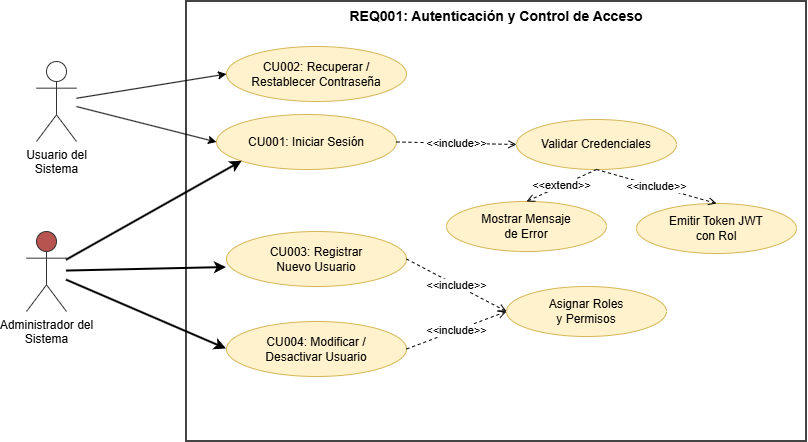
\includegraphics[width=\linewidth]{imagenes/REQ001.png}
\end{figure}

{
\small
\setstretch{1.15}
\setlength{\parindent}{0pt}
\begin{xltabular}{\linewidth}{
    >{\raggedright\arraybackslash}p{3.5cm} 
    >{\raggedright\arraybackslash}X
}
    % --- Encabezado de la primera página ---
    \caption{Especificación del Caso de Uso - REQ001} \label{tab:spec_req001} \\
    \toprule
    \textbf{ID. Req.:} REQ001 & \textbf{ID. Caso de Uso:} CU001 - CU004 \\
    \midrule
    \endfirsthead

    % --- Encabezado en páginas siguientes ---
    \toprule
    \textbf{ID. Req.:} REQ001 & \textbf{ID. Caso de Uso:} CU001 - CU004 \\
    \midrule
    \endhead

    % --- Cierre en página intermedia ---
    \bottomrule
    \endfoot

    % --- Cierre final ---
    \bottomrule
    \endlastfoot

    % --- Filas de contenido ---
    \textbf{Descripción:} & Este caso de uso valida el acceso seguro al sistema mediante credenciales y asigna permisos específicos según el rol. \\
    \midrule
    \textbf{Secuencia Normal:} & 
    1. El usuario ingresa sus credenciales en la pantalla de inicio de sesión. \newline
    2. El sistema valida usuario y contraseña (\textit{si son incorrectos, ver Excepción 1}). \newline
    3. El sistema verifica que la cuenta esté activa (\textit{si está inactiva, ver Excepción 2}). \newline
    4. El sistema genera el token de sesión y aplica el rol autorizado. \newline
    5. El sistema muestra el panel principal con los módulos permitidos. \\
    \midrule
    \textbf{Excepciones:} & 
    \textbf{Excepción 1 (Credenciales incorrectas):} El sistema muestra una advertencia, limpia los campos y retorna al paso 1 de la secuencia normal. \newline
    \textbf{Excepción 2 (Usuario inactivo):} El sistema informa que la cuenta está deshabilitada, finaliza el flujo y conserva al usuario en la pantalla de acceso. \\
\end{xltabular}
}

% ---------------------------------------------------------
% REQ002
% ---------------------------------------------------------
\paragraph{REQ002: Importación y Gestión de Archivos SAT (FEL)}
Describe la carga masiva e importación de facturas electrónicas desde los archivos proporcionados por la SAT (XML/Excel), la extracción de metadatos fiscales y la centralización de comprobantes.


\begin{figure}[H]
    \centering
    \caption{REQ002: Importación y Gestión de Archivos SAT (FEL)}
    \label{fig:REQ002}
    \vspace{0.2cm}
    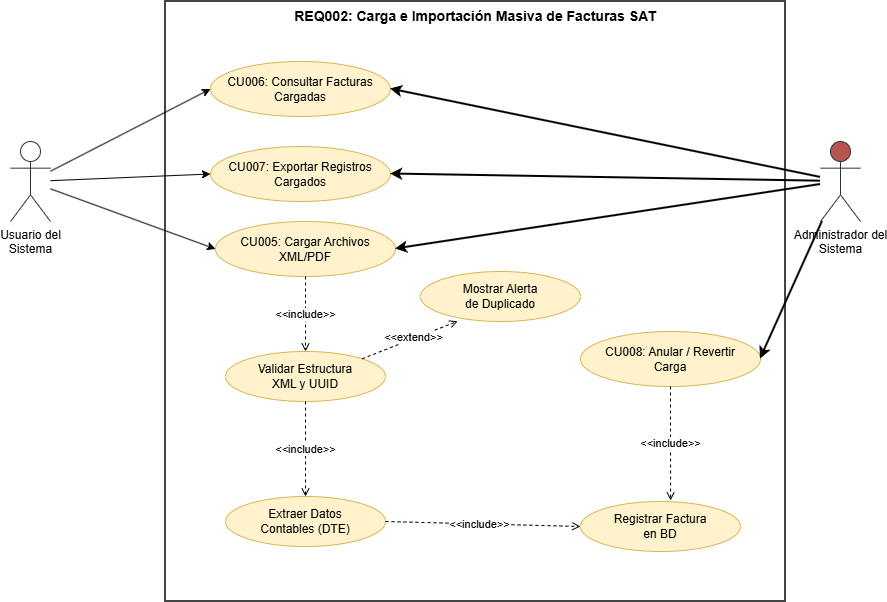
\includegraphics[width=\linewidth]{imagenes/REQ002.png}
\end{figure}

{
\small
\setstretch{1.15}
\setlength{\parindent}{0pt}
\begin{xltabular}{\linewidth}{
    >{\raggedright\arraybackslash}p{3.5cm} 
    >{\raggedright\arraybackslash}X
}
    % --- Encabezado de la primera página ---
    \caption{Especificación del Caso de Uso - REQ002} \label{tab:spec_req002} \\
    \toprule
    \textbf{ID. Req.:} REQ002 & \textbf{ID. Caso de Uso:} CU005 - CU008 \\
    \midrule
    \endfirsthead

    % --- Encabezado en páginas siguientes ---
    \toprule
    \textbf{ID. Req.:} REQ002 & \textbf{ID. Caso de Uso:} CU005 - CU008 \\
    \midrule
    \endhead

    % --- Cierre en página intermedia ---
    \bottomrule
    \endfoot

    % --- Cierre final ---
    \bottomrule
    \endlastfoot

    % --- Filas de contenido ---
    \textbf{Descripción:} & Permite procesar masivamente los reportes mensuales de la SAT, extrayendo metadatos fiscales y centralizando las facturas en la base de datos. \\
    \midrule
    \textbf{Secuencia Normal:} & 
    1. El usuario selecciona y carga el archivo Excel/XML de la SAT (\textit{si el formato no es válido, ver Excepción 1}). \newline
    2. El sistema extrae NIT, nombre, autorización, fecha, monto, IVA y concepto. \newline
    3. El sistema verifica duplicidad y clasifica las facturas (\textit{si existe duplicidad, ver Excepción 2}). \newline
    4. El usuario confirma la carga y el sistema registra las facturas disponibles para Proveedores, Caja chica o Viáticos. \\
    \midrule
    \textbf{Excepciones:} & 
    \textbf{1. Formato no válido:} El sistema informa el error y retorna al paso 1 para seleccionar un archivo válido. \newline
    \textbf{2. Factura duplicada:} El sistema omite el registro, continúa en el paso 2 con la siguiente fila y genera el resumen de omisiones. \newline
    \textbf{3. Concepto no clasificado:} El usuario asigna una cuenta de nomenclatura y el flujo retorna al paso 4. \\
\end{xltabular}
}

% ---------------------------------------------------------
% REQ003
% ---------------------------------------------------------
\paragraph{REQ003: Emisión y Control de Cheques Postfechados}
Ilustra la gestión de cheques emitidos a fecha futura, la asignación de fechas de cobro, el seguimiento de estados (Emitido, Depositado, Anulado) y la programación en calendario.

\begin{figure}[H]
    \centering
    \caption{REQ003: Emisión y Control de Cheques Postfechados}
    \label{fig:REQ003}
    \vspace{0.2cm}
    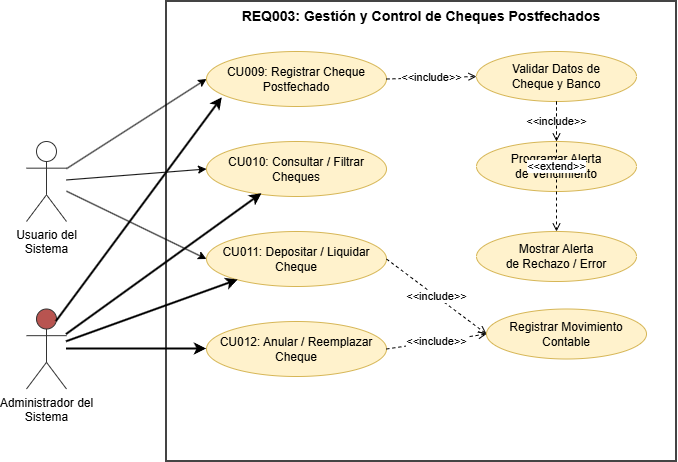
\includegraphics[width=\linewidth]{imagenes/REQ003.png}
\end{figure}

{
\small
\setstretch{1.15}
\setlength{\parindent}{0pt}
\begin{xltabular}{\linewidth}{
    >{\raggedright\arraybackslash}p{3.5cm} 
    >{\raggedright\arraybackslash}X
}
    % --- Encabezado de la primera página ---
    \caption{Especificación del Caso de Uso - REQ003} \label{tab:spec_req003} \\
    \toprule
    \textbf{ID. Req.:} REQ003 & \textbf{ID. Caso de Uso:} CU009 - CU012 \\
    \midrule
    \endfirsthead

    % --- Encabezado en páginas siguientes ---
    \toprule
    \textbf{ID. Req.:} REQ003 & \textbf{ID. Caso de Uso:} CU009 - CU012 \\
    \midrule
    \endhead

    % --- Cierre en página intermedia ---
    \bottomrule
    \endfoot

    % --- Cierre final ---
    \bottomrule
    \endlastfoot

    % --- Filas de contenido ---
    \textbf{Descripción:} & Automatiza el control de cheques recibidos/emitidos con fecha posterior, ajustando sus fechas de depósito a días hábiles. \\
    \midrule
    \textbf{Secuencia Normal:} & 
    1. El usuario registra cliente, banco del cheque, banco de depósito, número, monto y fechas (\textit{si faltan datos, ver Excepción 1}). \newline
    2. El sistema verifica que el número de cheque no esté registrado (\textit{si existe, ver Excepción 1}). \newline
    3. El sistema asigna estado Pendiente y ajusta la fecha de depósito a un día hábil. \newline
    4. El sistema guarda el cheque y lo incorpora al calendario (\textit{si es rechazado, ver Excepción 2}). \\
    \midrule
    \textbf{Excepciones:} & 
    \textbf{1. Cheque duplicado o incompleto:} El sistema informa el problema y retorna al paso 1 para corregir los datos. \newline
    \textbf{2. Cheque rechazado:} El usuario registra recepción del rechazo y una nueva fecha; el flujo retorna al paso 4 para actualizar el calendario. \\
\end{xltabular}
}

% ---------------------------------------------------------
% REQ004
% ---------------------------------------------------------
\paragraph{REQ004: Creación y Control de Fondo de Caja Chica}
Aborda la asignación de facturas SAT y comprobantes no fiscales (vales/recibos), la ejecución de cálculos contables automatizados y la generación de borradores de partidas de diario.

\begin{figure}[H]
    \centering
    \caption{REQ004: Creación y Control de Fondo de Caja Chica}
    \label{fig:REQ004}
    \vspace{0.2cm}
    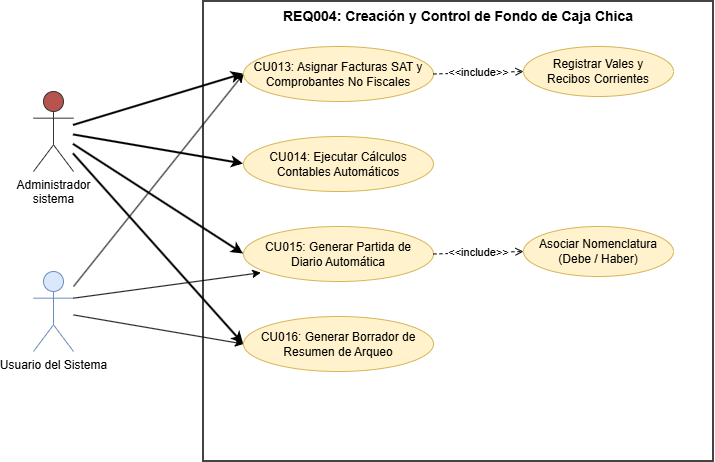
\includegraphics[width=\linewidth]{imagenes/REQ004.png}
\end{figure}

{
\small
\setstretch{1.15}
\setlength{\parindent}{0pt}
\begin{xltabular}{\linewidth}{
    >{\raggedright\arraybackslash}p{3.5cm} 
    >{\raggedright\arraybackslash}X
}
    % --- Encabezado de la primera página ---
    \caption{Especificación del Caso de Uso - REQ004} \label{tab:spec_req004} \\
    \toprule
    \textbf{ID. Req.:} REQ004 & \textbf{ID. Caso de Uso:} CU013 - CU016 \\
    \midrule
    \endfirsthead

    % --- Encabezado en páginas siguientes ---
    \toprule
    \textbf{ID. Req.:} REQ004 & \textbf{ID. Caso de Uso:} CU013 - CU016 \\
    \midrule
    \endhead

    % --- Cierre en página intermedia ---
    \bottomrule
    \endfoot

    % --- Cierre final ---
    \bottomrule
    \endlastfoot

    % --- Filas de contenido ---
    \textbf{Descripción:} & Gestiona los desembolsos de caja chica agrupando comprobantes fiscales y vales internos, generando partidas automáticas. \\
    \midrule
    \textbf{Secuencia Normal:} & 
    1. El auxiliar llama una factura FEL por número o registra un Recibo/otro documento. \newline
    2. El sistema muestra el movimiento y propone una cuenta de nomenclatura (\textit{si no reconoce el concepto, ver Excepción 1}). \newline
    3. El usuario confirma o asigna la cuenta contable y el sistema calcula gastos, IVA y total. \newline
    4. El sistema genera la partida contable y el resumen imprimible de Caja chica. \\
    \midrule
    \textbf{Excepciones:} & 
    \textbf{1. Factura asignada a otro módulo:} El sistema informa el bloqueo y retorna al paso 1 para seleccionar otro comprobante. \newline
    \textbf{2. Cuenta no reconocida:} Se despliega el selector de nomenclatura; al elegir una cuenta, el flujo retorna al paso 3. \newline
    \textbf{3. Debe y Haber descuadrados:} El sistema detiene la generación y retorna al paso 3 para corregir la cuenta o el monto. \\
\end{xltabular}
}

% ---------------------------------------------------------
% REQ005
% ---------------------------------------------------------
\paragraph{REQ005: Liquidación y Reintegro de Viáticos}
Muestra el flujo de asociación de facturas físicas por colaborador mediante número correlativo, la programación de giras organizadas por semanas calendario y el cálculo de reembolsos.


\begin{figure}[H]
    \centering
    \caption{REQ005: Liquidación y Reintegro de Viáticos}
    \label{fig:REQ005}
    \vspace{0.2cm}
    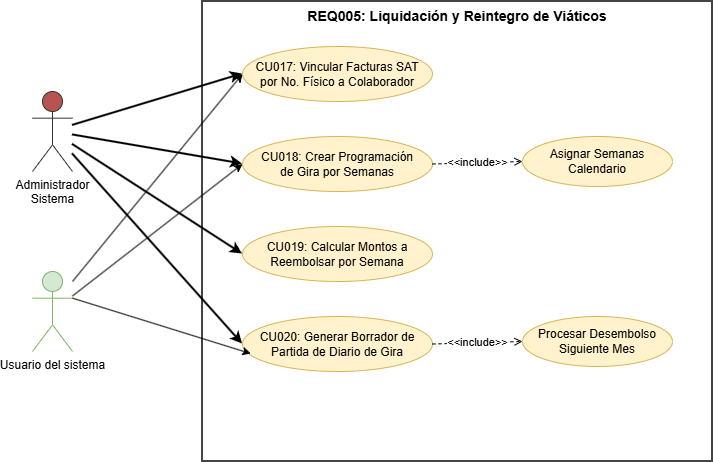
\includegraphics[width=\linewidth]{imagenes/REQ005.png}
\end{figure}

{
\small
\setstretch{1.15}
\setlength{\parindent}{0pt}
\begin{xltabular}{\linewidth}{
    >{\raggedright\arraybackslash}p{3.5cm} 
    >{\raggedright\arraybackslash}X
}
    % --- Encabezado de la primera página ---
    \caption{Especificación del Caso de Uso - REQ005} \label{tab:spec_req005} \\
    \toprule
    \textbf{ID. Req.:} REQ005 & \textbf{ID. Caso de Uso:} CU017 - CU020 \\
    \midrule
    \endfirsthead

    % --- Encabezado en páginas siguientes ---
    \toprule
    \textbf{ID. Req.:} REQ005 & \textbf{ID. Caso de Uso:} CU017 - CU020 \\
    \midrule
    \endhead

    % --- Cierre en página intermedia ---
    \bottomrule
    \endfoot

    % --- Cierre final ---
    \bottomrule
    \endlastfoot

    % --- Filas de contenido ---
    \textbf{Descripción:} & Controla las liquidaciones de viáticos de los colaboradores, vinculando sus facturas entregadas con la programación de giras. \\
    \midrule
    \textbf{Secuencia Normal:} & 
    1. El usuario selecciona colaborador, territorio y semana de gira 1 a 5. \newline
    2. El usuario asigna facturas por número a Viáticos, Movilidad, Actividades o Bonos/otros gastos (\textit{si no se reconoce la cuenta, ver Excepción 1}). \newline
    3. El sistema calcula los gastos de la liquidación y aplica la regla de Movilidad de la primera semana. \newline
    4. El sistema genera la partida semanal o transitoria según la fecha y el estado de reintegro. \\
    \midrule
    \textbf{Excepciones:} & 
    \textbf{1. Factura no encontrada:} El sistema informa el resultado y retorna al paso 2 para buscar otro número o cargar la factura. \newline
    \textbf{2. Factura asignada a otro módulo:} Se bloquea la vinculación y el flujo retorna al paso 2 para seleccionar otro comprobante. \newline
    \textbf{3. Semana no válida para Movilidad:} El sistema informa que Movilidad corresponde a la semana 1 y retorna al paso 1. \\
\end{xltabular}
}

% ---------------------------------------------------------
% REQ006
% ---------------------------------------------------------
\paragraph{REQ006: Programación de Pagos a Proveedores}
Establece la gestión de la ficha del proveedor (días de crédito y retenciones IVA/ISR), la vinculación con facturas de la SAT y el cálculo automático de fechas de vencimiento.


\begin{figure}[H]
    \centering
    \caption{REQ006: Programación de Pagos a Proveedores}
    \label{fig:REQ006}
    \vspace{0.2cm}
    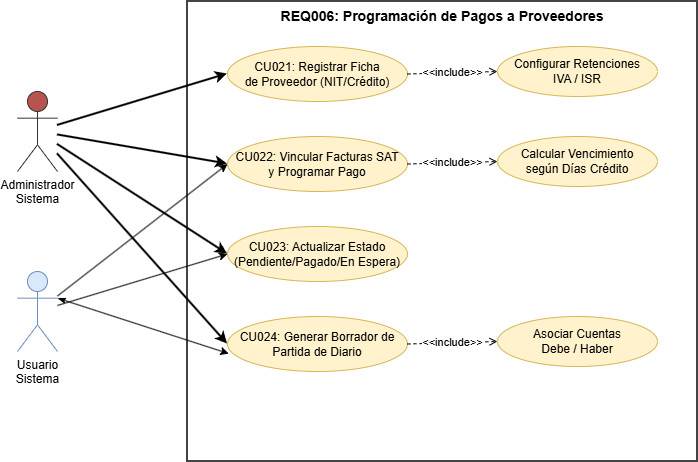
\includegraphics[width=\linewidth]{imagenes/REQ006.png}
\end{figure}

{
\small
\setstretch{1.15}
\setlength{\parindent}{0pt}
\begin{xltabular}{\linewidth}{
    >{\raggedright\arraybackslash}p{3.5cm} 
    >{\raggedright\arraybackslash}X
}
    % --- Encabezado de la primera página ---
    \caption{Especificación del Caso de Uso - REQ006} \label{tab:spec_req006} \\
    \toprule
    \textbf{ID. Req.:} REQ006 & \textbf{ID. Caso de Uso:} CU021 - CU024 \\
    \midrule
    \endfirsthead

    % --- Encabezado en páginas siguientes ---
    \toprule
    \textbf{ID. Req.:} REQ006 & \textbf{ID. Caso de Uso:} CU021 - CU024 \\
    \midrule
    \endhead

    % --- Cierre en página intermedia ---
    \bottomrule
    \endfoot

    % --- Cierre final ---
    \bottomrule
    \endlastfoot

    % --- Filas de contenido ---
    \textbf{Descripción:} & Administra los compromisos comerciales con proveedores a crédito, calculando vencimientos y reteniendo impuestos según ley. \\
    \midrule
    \textbf{Secuencia Normal:} & 
    1. El usuario registra NIT, días de crédito, retenciones y cuenta de nomenclatura del proveedor. \newline
    2. El sistema completa los nombres y despliega las facturas del proveedor por mes. \newline
    3. El sistema calcula vencimiento, retenciones y descuentos (\textit{si el vencimiento cruza el mes, ver Excepción 2}). \newline
    4. El usuario genera la partida dentro del mes o la partida transitoria con gastos e IVA en Debe y retenciones/descuentos en Haber. \\
    \midrule
    \textbf{Excepciones:} & 
    \textbf{1. Proveedor no registrado:} El sistema solicita crear la ficha y retorna al paso 1. \newline
    \textbf{2. Factura previamente pagada o anulada:} El sistema bloquea el procesamiento y retorna al paso 2 para seleccionar otra factura. \newline
    \textbf{3. Vencimiento fuera del mes:} El sistema dirige la factura a Cuenta transitoria y retorna al paso 4 para generar la partida correspondiente. \\
\end{xltabular}
}

% ---------------------------------------------------------
% REQ007
% ---------------------------------------------------------
\paragraph{REQ007: Módulo de Calendario Dinámico y Programación Operativa}
Consolida en una interfaz visual e interactiva las fechas de cobro de cheques, vencimientos de proveedores y liquidaciones de viáticos, permitiendo reprogramaciones en tiempo real.

\begin{figure}[H]
    \centering
    \caption{REQ007: Módulo de Calendario Dinámico y Programación Operativa}
    \label{fig:REQ007}
    \vspace{0.2cm}
    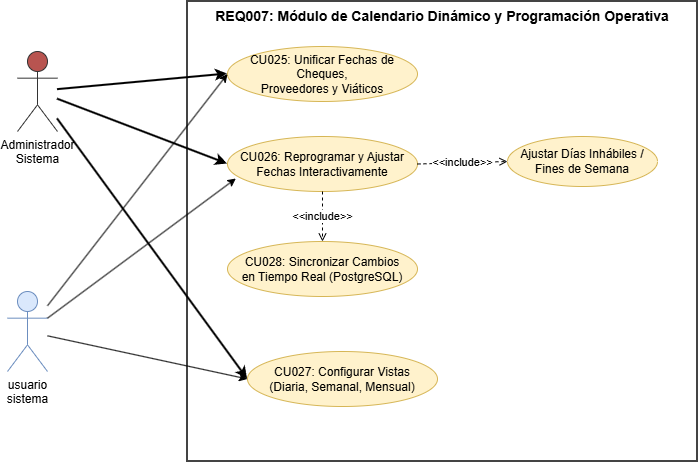
\includegraphics[width=\linewidth]{imagenes/REQ007.png}
\end{figure}

{
\small
\setstretch{1.15}
\setlength{\parindent}{0pt}
\begin{xltabular}{\linewidth}{
    >{\raggedright\arraybackslash}p{3.5cm} 
    >{\raggedright\arraybackslash}X
}
    % --- Encabezado de la primera página ---
    \caption{Especificación del Caso de Uso - REQ007} \label{tab:spec_req007} \\
    \toprule
    \textbf{ID. Req.:} REQ007 & \textbf{ID. Caso de Uso:} CU025 - CU028 \\
    \midrule
    \endfirsthead

    % --- Encabezado en páginas siguientes ---
    \toprule
    \textbf{ID. Req.:} REQ007 & \textbf{ID. Caso de Uso:} CU025 - CU028 \\
    \midrule
    \endhead

    % --- Cierre en página intermedia ---
    \bottomrule
    \endfoot

    % --- Cierre final ---
    \bottomrule
    \endlastfoot

    % --- Filas de contenido ---
    \textbf{Descripción:} & Ofrece una vista consolidada de los compromisos contables del mes con capacidad de edición directa mediante interfaz gráfica. \\
    \midrule
    \textbf{Secuencia Normal:} & 
    1. El sistema recupera las actividades de cheques, proveedores y viáticos. \newline
    2. El usuario consulta la agenda en vista mensual, semanal o diaria. \newline
    3. El usuario selecciona una actividad y solicita reprogramación (\textit{si cae en día inhábil, ver Excepción 1}). \newline
    4. El sistema guarda la nueva fecha y actualiza la vista del calendario. \\
    \midrule
    \textbf{Excepciones:} & 
    \textbf{1. Reprogramación en día inhábil:} El sistema propone el día hábil más cercano y retorna al paso 3 para confirmar. \newline
    \textbf{2. Error de conexión:} Se informa el error, se conserva la fecha anterior y se retorna al paso 3 para reintentar. \newline
    \textbf{3. Sin actividad registrada:} El sistema muestra el calendario vacío y retorna al paso 1 para ajustar el período. \\
\end{xltabular}
}

% ---------------------------------------------------------
% REQ008
% ---------------------------------------------------------
\paragraph{REQ008: Nomenclatura Contable y Partidas Automáticas}
Detalla la estructura del catálogo de cuentas contables, la parametrización de reglas para el Debe y el Haber, y la construcción del borrador de la partida contable.

\begin{figure}[H]
    \centering
    \caption{REQ008: Nomenclatura Contable y Partidas Automáticas}
    \label{fig:REQ008}
    \vspace{0.2cm}
    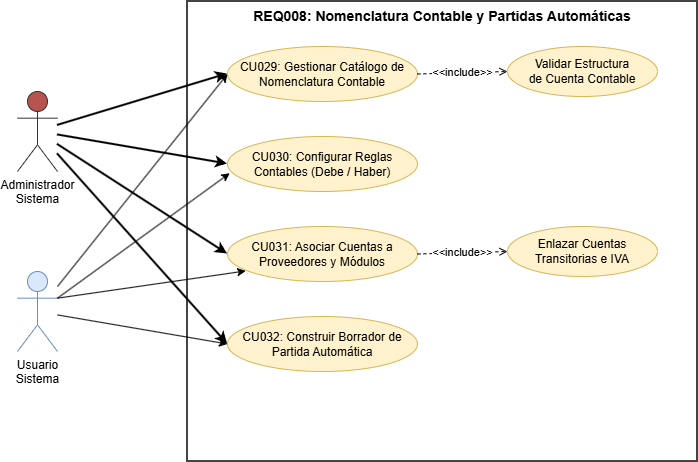
\includegraphics[width=\linewidth]{imagenes/REQ008.png}
\end{figure}

{
\small
\setstretch{1.15}
\setlength{\parindent}{0pt}
\begin{xltabular}{\linewidth}{
    >{\raggedright\arraybackslash}p{3.5cm} 
    >{\raggedright\arraybackslash}X
}
    % --- Encabezado de la primera página ---
    \caption{Especificación del Caso de Uso - REQ008} \label{tab:spec_req008} \\
    \toprule
    \textbf{ID. Req.:} REQ008 & \textbf{ID. Caso de Uso:} CU029 - CU032 \\
    \midrule
    \endfirsthead

    % --- Encabezado en páginas siguientes ---
    \toprule
    \textbf{ID. Req.:} REQ008 & \textbf{ID. Caso de Uso:} CU029 - CU032 \\
    \midrule
    \endhead

    % --- Cierre en página intermedia ---
    \bottomrule
    \endfoot

    % --- Cierre final ---
    \bottomrule
    \endlastfoot

    % --- Filas de contenido ---
    \textbf{Descripción:} & Define la parametrización contable del sistema garantizando la correcta generación de asientos balanceados. \\
    \midrule
    \textbf{Secuencia Normal:} & 
    1. El administrador registra una cuenta con código, nombre y naturaleza Debe o Haber (\textit{si el código existe, ver Excepción 1}). \newline
    2. El sistema muestra la cuenta activa en el catálogo y la ofrece en los selectores de clasificación. \newline
    3. El usuario asigna cuentas a proveedores, Caja chica o Viáticos. \newline
    4. El sistema genera la partida y verifica que Debe y Haber coincidan (\textit{si no coinciden, ver Excepción 2}). \\
    \midrule
    \textbf{Excepciones:} & 
    \textbf{1. Código duplicado:} Se bloquea el guardado y el flujo retorna al paso 1 para ingresar otro código. \newline
    \textbf{2. Partida descuadrada (Debe $\neq$ Haber):} El sistema resalta la diferencia y retorna al paso 4 para corregir la clasificación. \newline
    \textbf{3. Cuenta inactiva:} El selector la excluye y el flujo retorna al paso 2 para elegir una cuenta activa. \\
\end{xltabular}
}

% ---------------------------------------------------------
% REQ009
% ---------------------------------------------------------
\paragraph{REQ009: Generación de Reportes Operativos y Financieros}
Contempla la extracción y consolidación de reportes de cheques postfechados, proyecciones a proveedores, arqueos de caja chica y gastos de viáticos por colaborador.

\begin{figure}[H]
    \centering
    \caption{REQ009: Generación de Reportes Operativos y Financieros}
    \label{fig:REQ009}
    \vspace{0.2cm}
    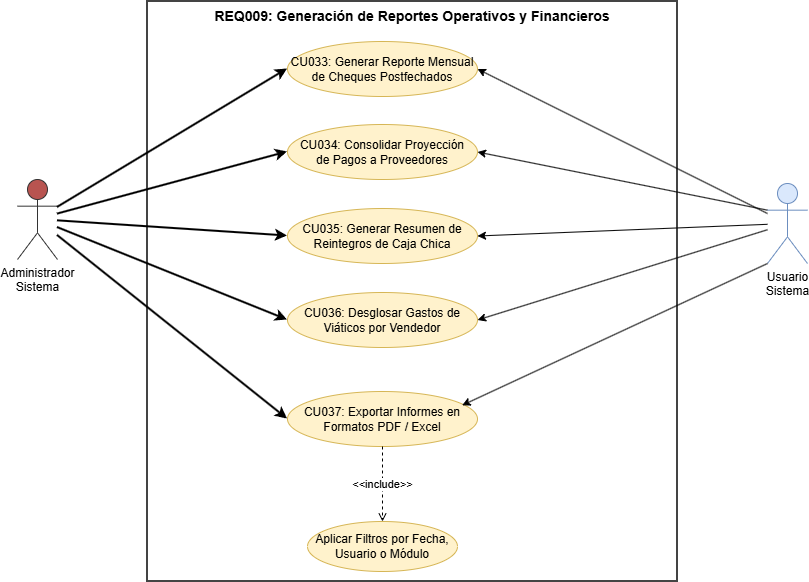
\includegraphics[width=\linewidth]{imagenes/REQ009.png}
\end{figure}

{
\small
\setstretch{1.15}
\setlength{\parindent}{0pt}
\begin{xltabular}{\linewidth}{
    >{\raggedright\arraybackslash}p{3.5cm} 
    >{\raggedright\arraybackslash}X
}
    % --- Encabezado de la primera página ---
    \caption{Especificación del Caso de Uso - REQ009} \label{tab:spec_req009} \\
    \toprule
    \textbf{ID. Req.:} REQ009 & \textbf{ID. Caso de Uso:} CU033 - CU037 \\
    \midrule
    \endfirsthead

    % --- Encabezado en páginas siguientes ---
    \toprule
    \textbf{ID. Req.:} REQ009 & \textbf{ID. Caso de Uso:} CU033 - CU037 \\
    \midrule
    \endhead

    % --- Cierre en página intermedia ---
    \bottomrule
    \endfoot

    % --- Cierre final ---
    \bottomrule
    \endlastfoot

    % --- Filas de contenido ---
    \textbf{Descripción:} & Permite consultar y exportar resúmenes financieros y operativos filtrados por rangos de fechas o entidades. \\
    \midrule
    \textbf{Secuencia Normal:} & 
    1. El usuario selecciona el tipo de reporte y sus filtros (\textit{si no hay registros, ver Excepción 1}). \newline
    2. El sistema consulta y consolida la información de los módulos. \newline
    3. El usuario revisa la vista previa. \newline
    4. El usuario imprime o exporta el resultado (\textit{si falla la exportación, ver Excepción 2}). \\
    \midrule
    \textbf{Excepciones:} & 
    \textbf{1. Sin datos en el rango seleccionado:} El sistema informa la ausencia de registros y retorna al paso 1 para cambiar los filtros. \newline
    \textbf{2. Error de exportación:} Se informa el fallo y retorna al paso 4 para reintentar la impresión o exportación. \\
\end{xltabular}
}


\subsubsection{Base de Datos}
El diseño relacional para la base de datos PostgreSQL integra la estructura de tablas, tipos enumerados y restricciones de claves foráneas requeridas para garantizar la integridad referencial de los módulos del sistema.

\begin{figure}[H]
    \centering
    \caption{Diagrama de Base de Datos Relacional}
    \label{fig:diagramabd}
    \vspace{0.2cm}
    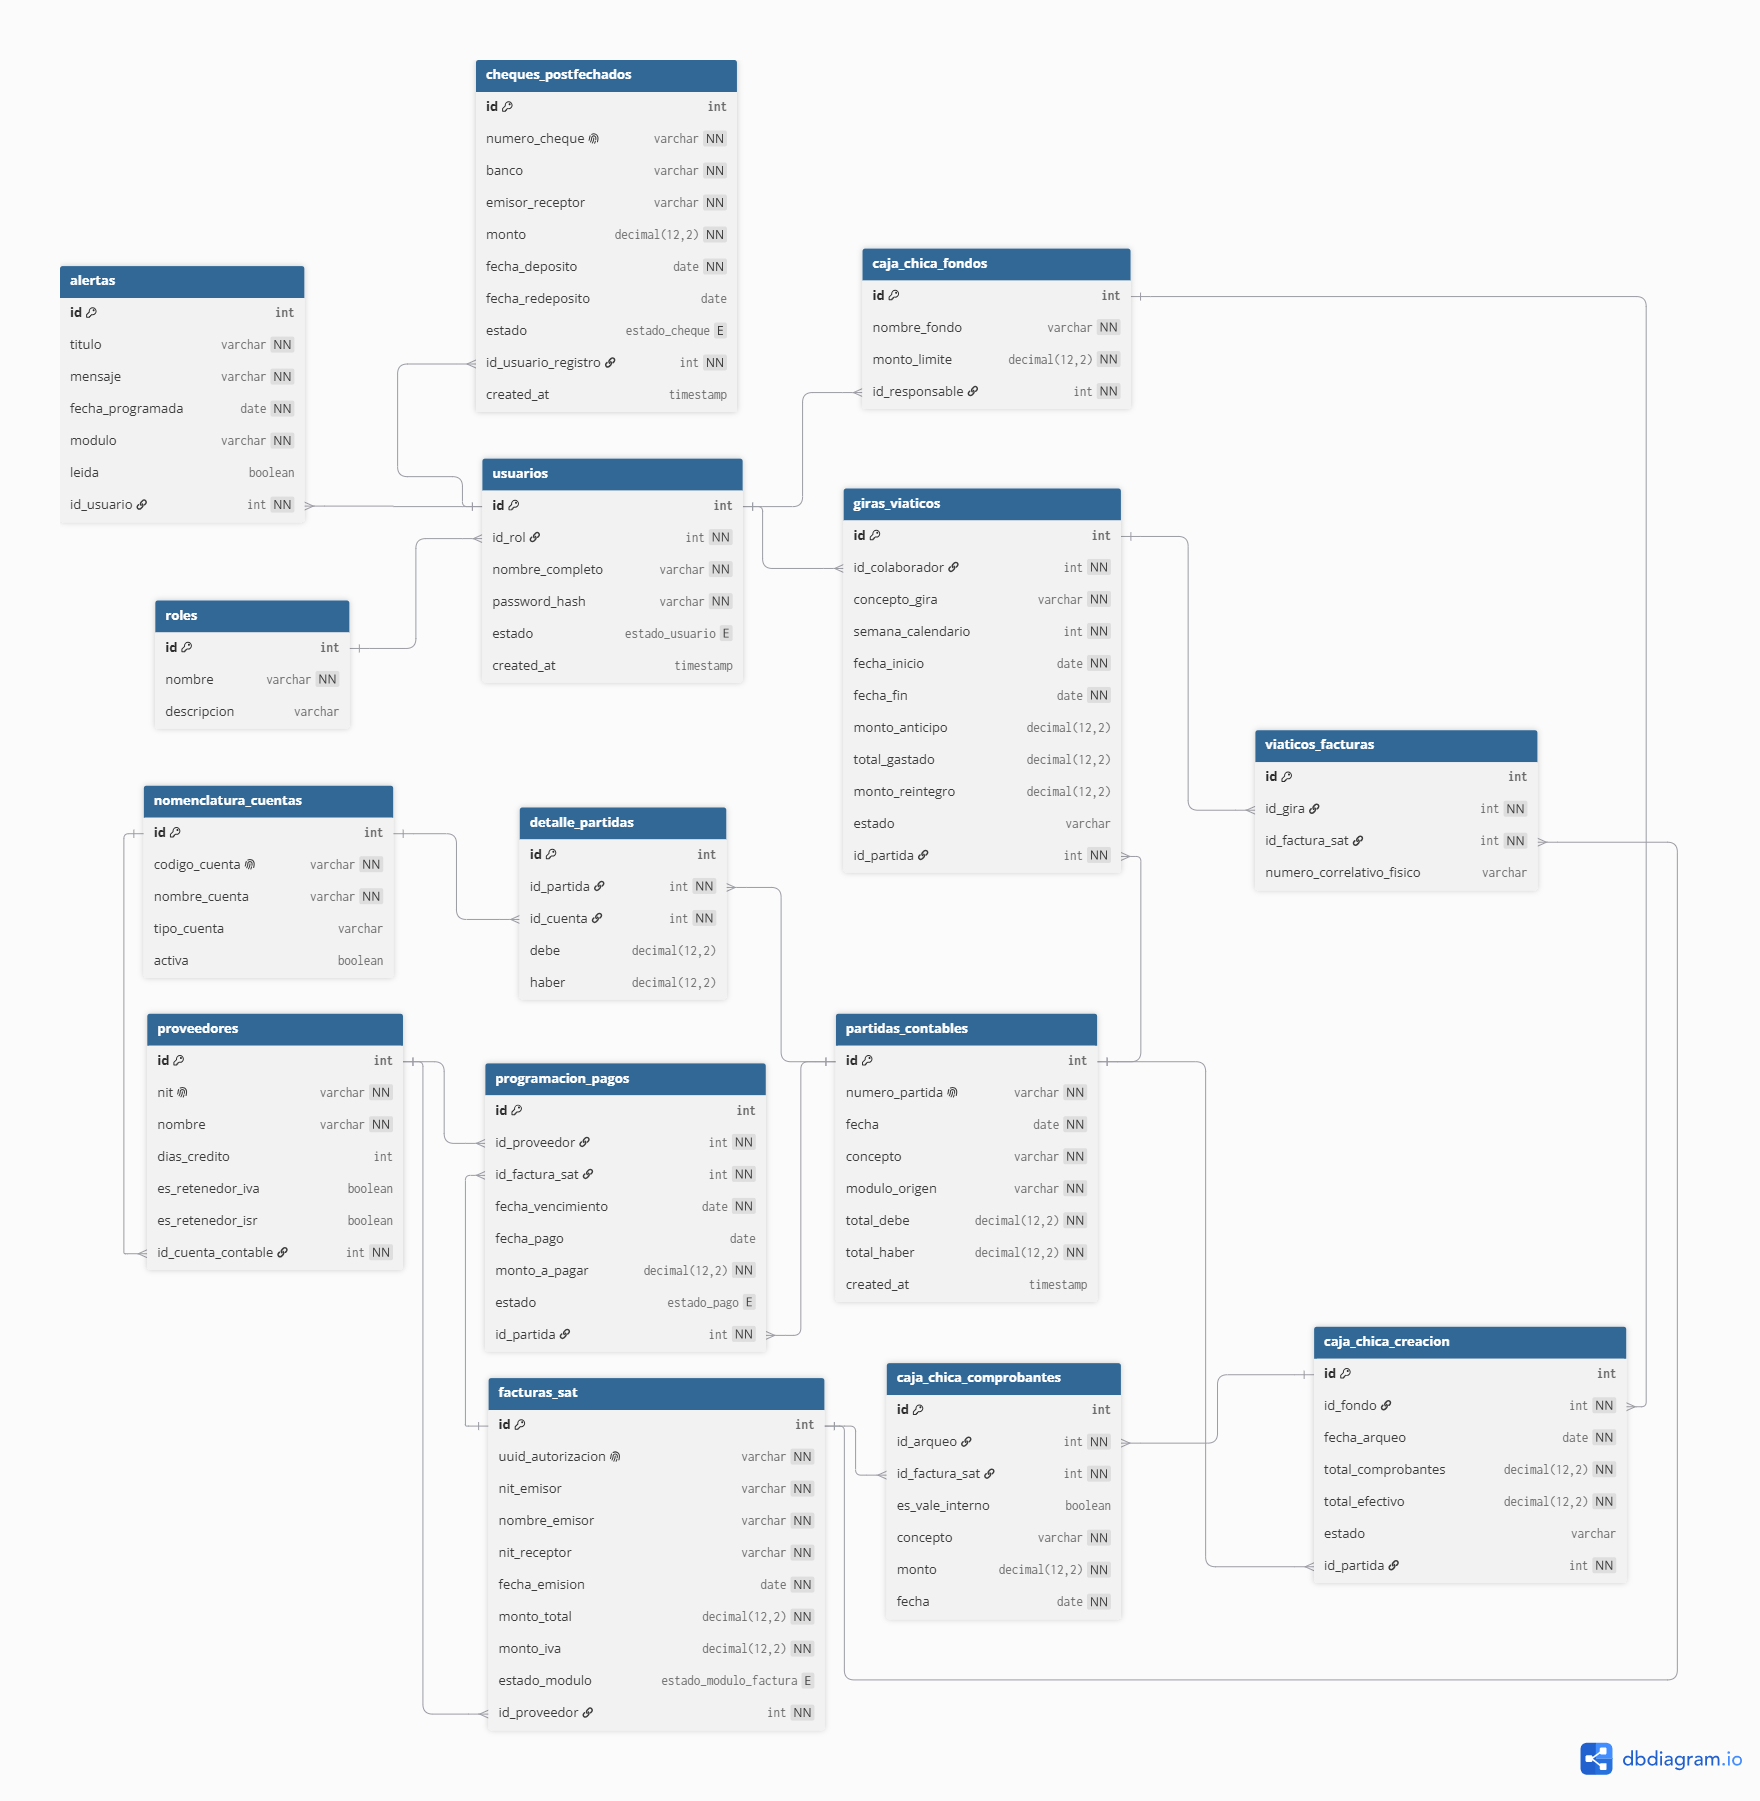
\includegraphics[width=\linewidth, height=\textheight, keepaspectratio]{imagenes/diagramabd.png}
    \vspace{0.2cm}
   
\end{figure}

\subsection{Diseño de Elementos}

La sección presenta los diseños visuales del Sistema Web y registra sus controles reutilizables. Las figuras se organizan por pantalla y por tipo de componente, evitando repetir nombres de botones o controles que aparecen en más de un módulo.

\subsubsection{Componentes visuales agrupados}

\begin{figure}[H]
    \centering
    \caption{Botones y acciones reutilizables del Sistema Web}
    \label{fig:componentes_botones}
    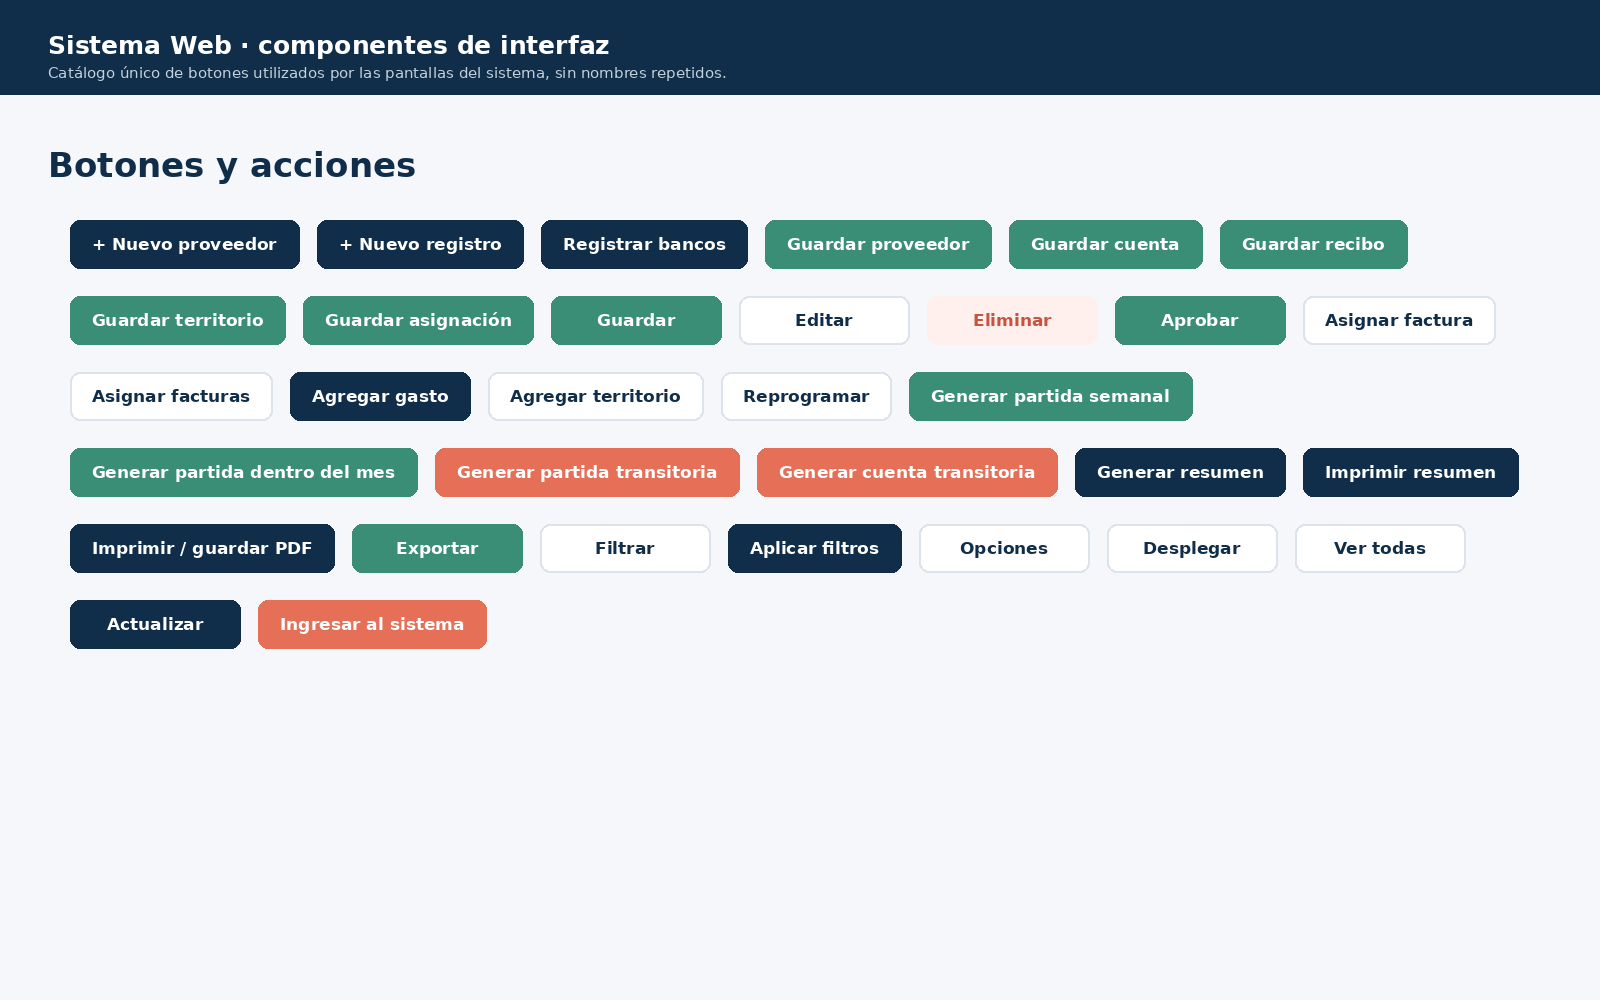
\includegraphics[width=0.96\linewidth]{imagenes/elementos_01_botones.png}
\end{figure}

\begin{figure}[H]
    \centering
    \caption{Listas desplegables y opciones de selección}
    \label{fig:componentes_listas}
    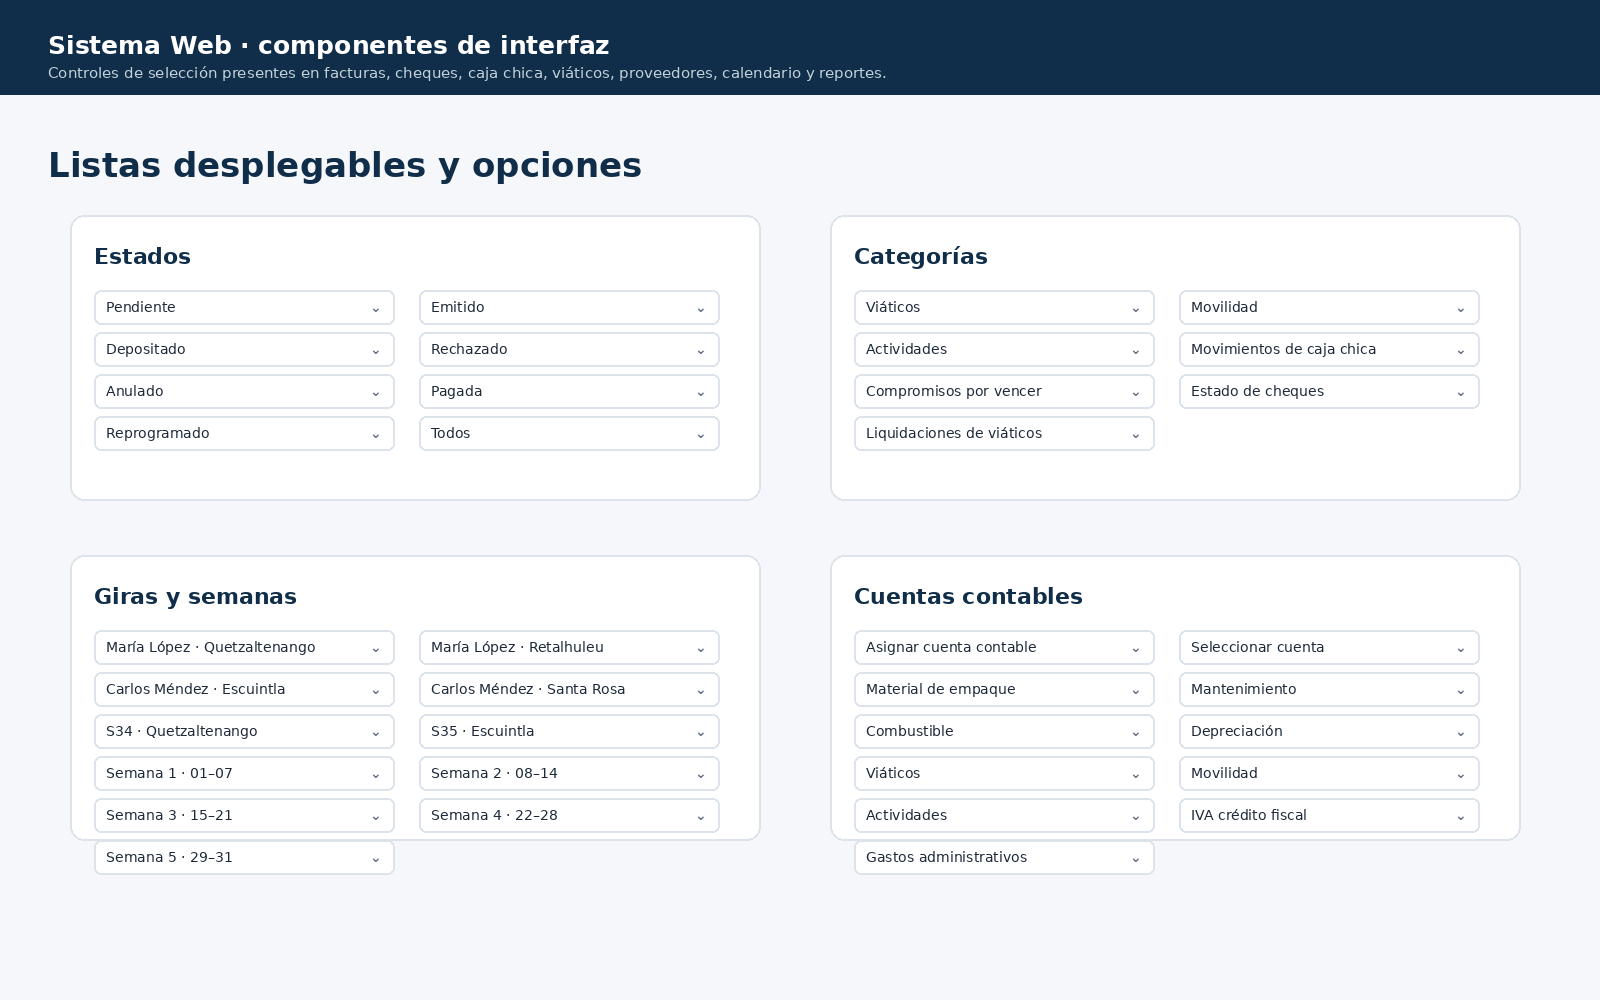
\includegraphics[width=0.96\linewidth]{imagenes/elementos_02_listas_desplegables.png}
\end{figure}

\begin{figure}[H]
    \centering
    \caption{Formularios y campos de captura}
    \label{fig:componentes_formularios}
    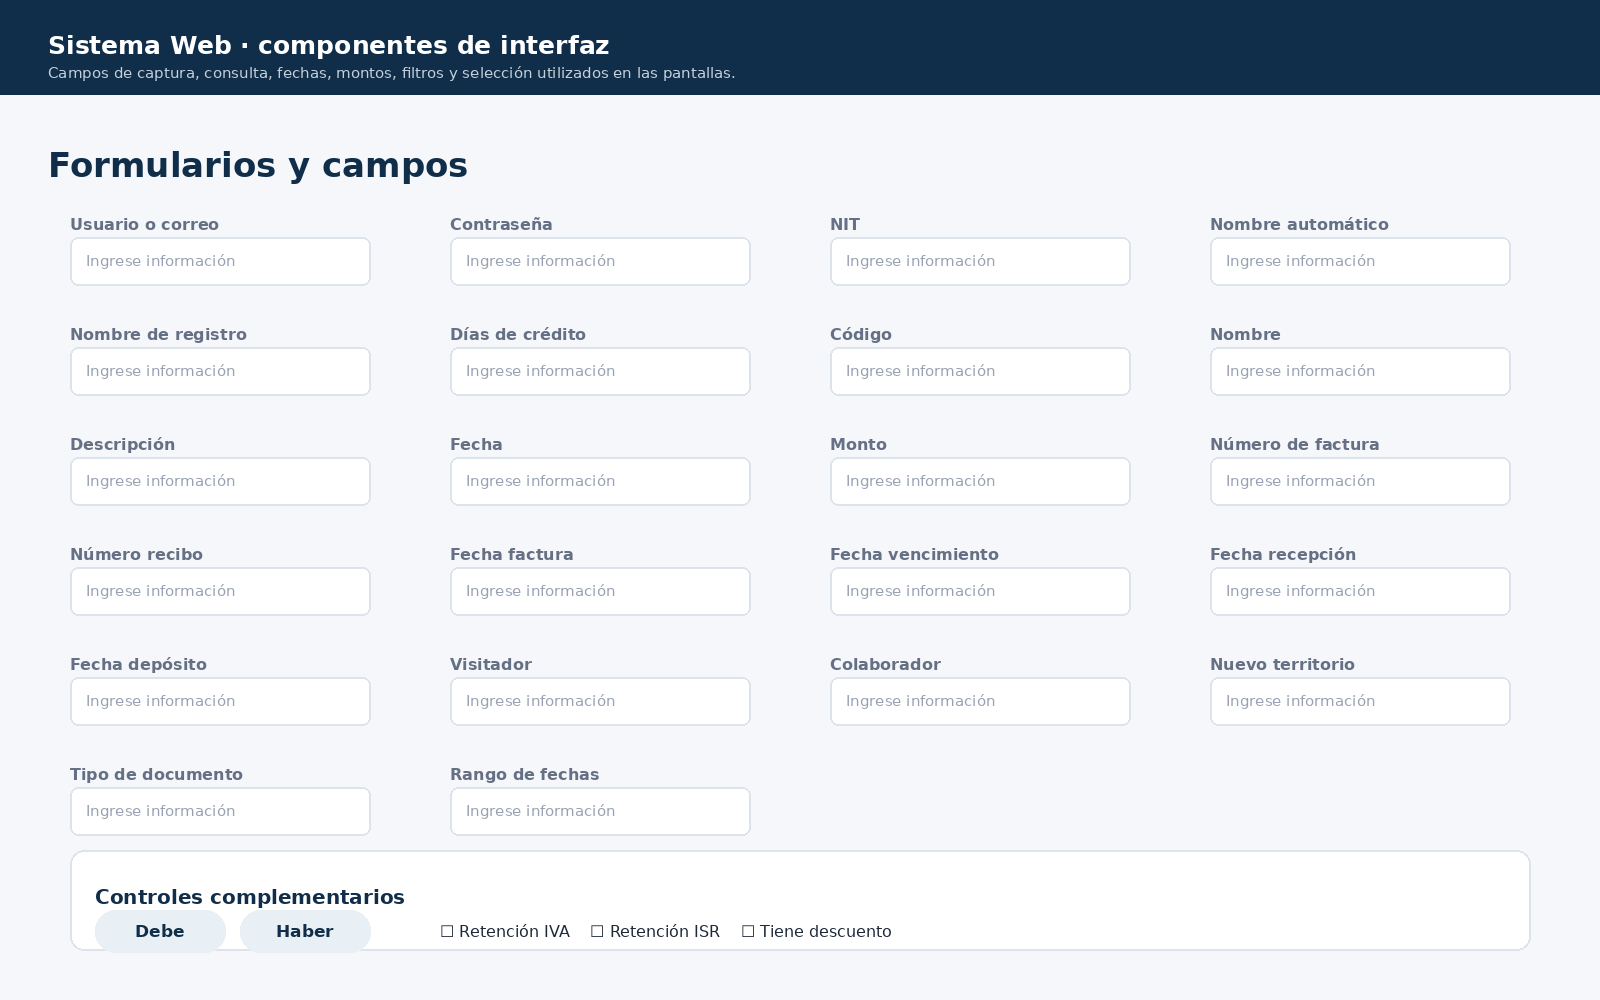
\includegraphics[width=0.96\linewidth]{imagenes/elementos_03_formularios.png}
\end{figure}

\begin{figure}[H]
    \centering
    \caption{Tablas, tarjetas y estados operativos}
    \label{fig:componentes_tablas}
    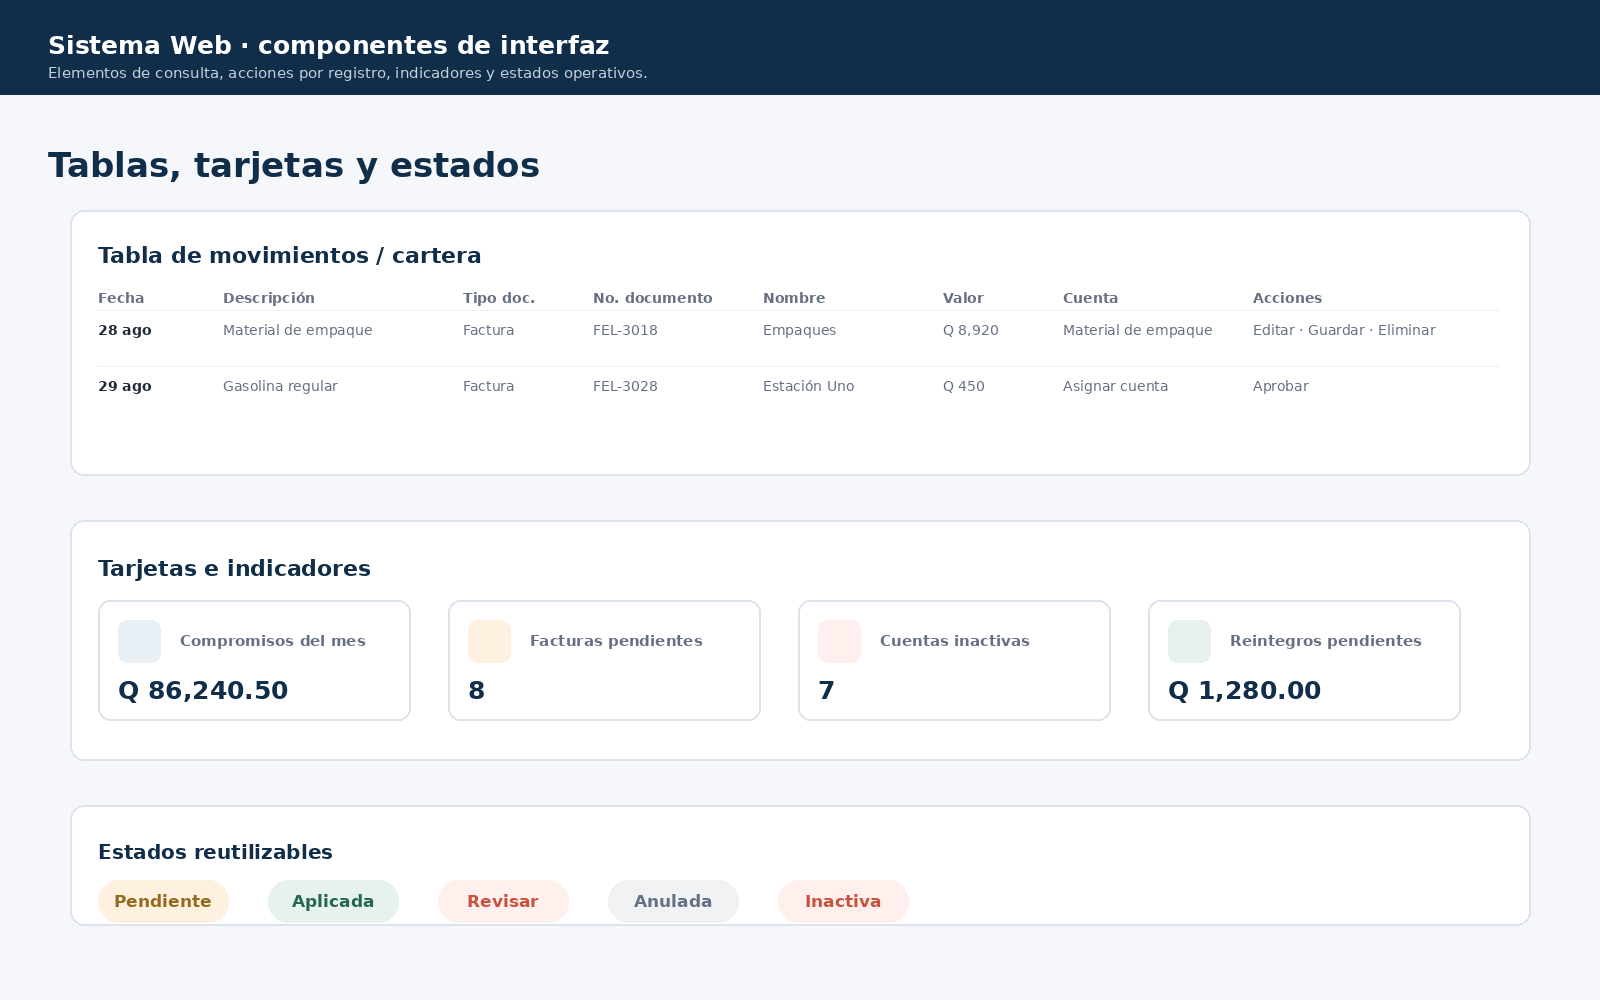
\includegraphics[width=0.96\linewidth]{imagenes/elementos_04_tablas_tarjetas.png}
\end{figure}

\begin{figure}[H]
    \centering
    \caption{Acciones contables, generación e impresión}
    \label{fig:componentes_contables}
    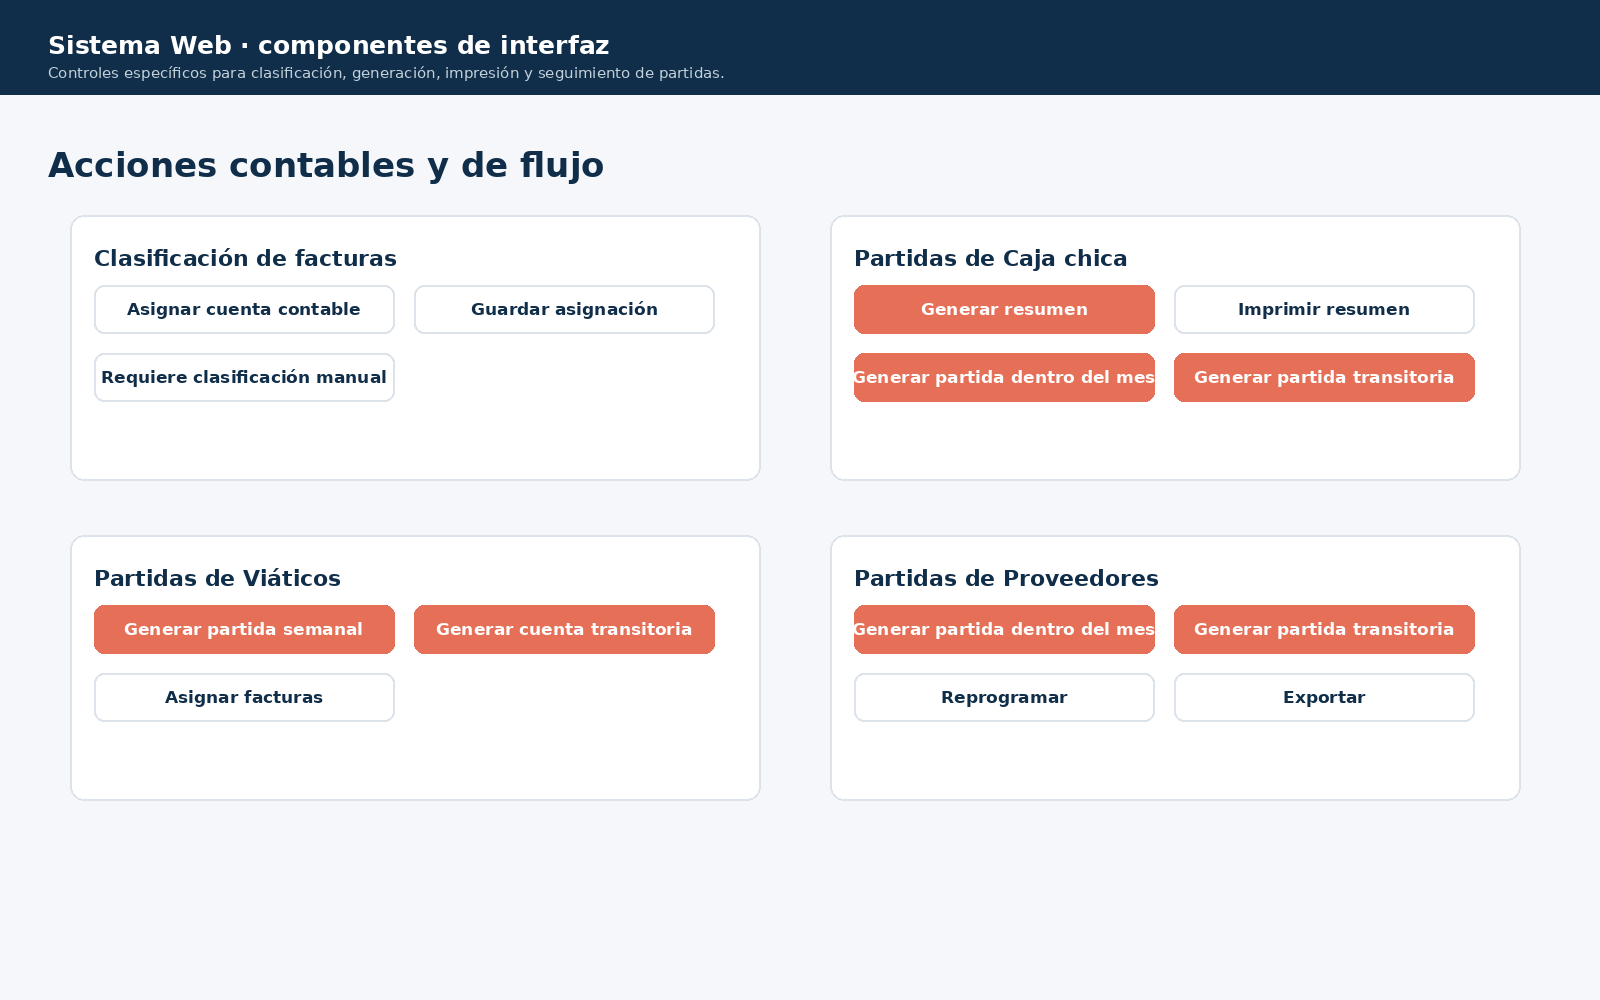
\includegraphics[width=0.96\linewidth]{imagenes/elementos_05_acciones_contables.png}
\end{figure}

\subsubsection{Diseños visuales individuales del sistema}

\begin{figure}[H]
    \centering
    \caption{Pantalla de inicio de sesión}
    \label{fig:pantalla_login}
    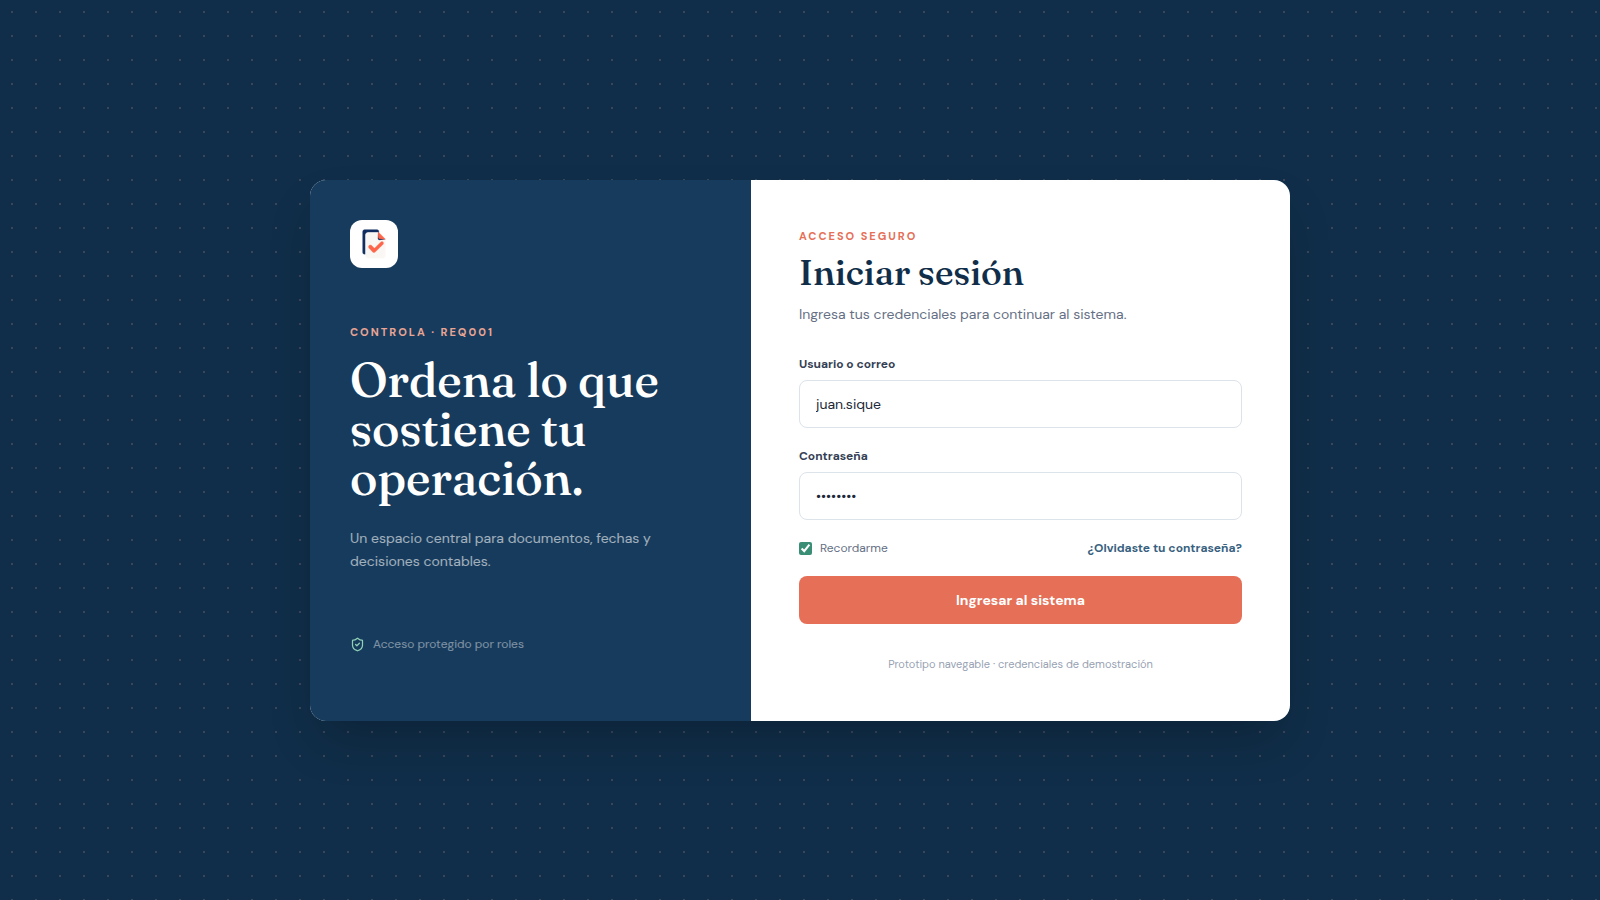
\includegraphics[width=0.96\linewidth]{imagenes/pantalla_01_login.png}
\end{figure}
\begin{table}[H]\centering
\caption{Descripción de Campos de la Pantalla de Autenticación de Usuarios}
\label{tab:3_12_pantalla_login}
\small\setstretch{1.15}
\begin{tabular}{p{0.25\linewidth}p{0.20\linewidth}p{0.20\linewidth}p{0.27\linewidth}}
\toprule
\textbf{Campo o control} & \textbf{Tipo} & \textbf{Valor por defecto} & \textbf{Observación} \\
\midrule
Usuario o correo & Entrada & Vacío & Campo requerido para ingresar el usuario. \\
Contraseña & Entrada protegida & Vacío & Campo requerido para validar el acceso. \\
Recordarme & Casilla & Desactivada & Conserva la sesión únicamente en un equipo autorizado. \\
Ingresar al sistema & Botón & Activo & Valida las credenciales y muestra el Panel principal. \\
\bottomrule
\end{tabular}
\end{table}


\begin{figure}[H]
    \centering
    \caption{Panel principal del Sistema Web}
    \label{fig:pantalla_dashboard}
    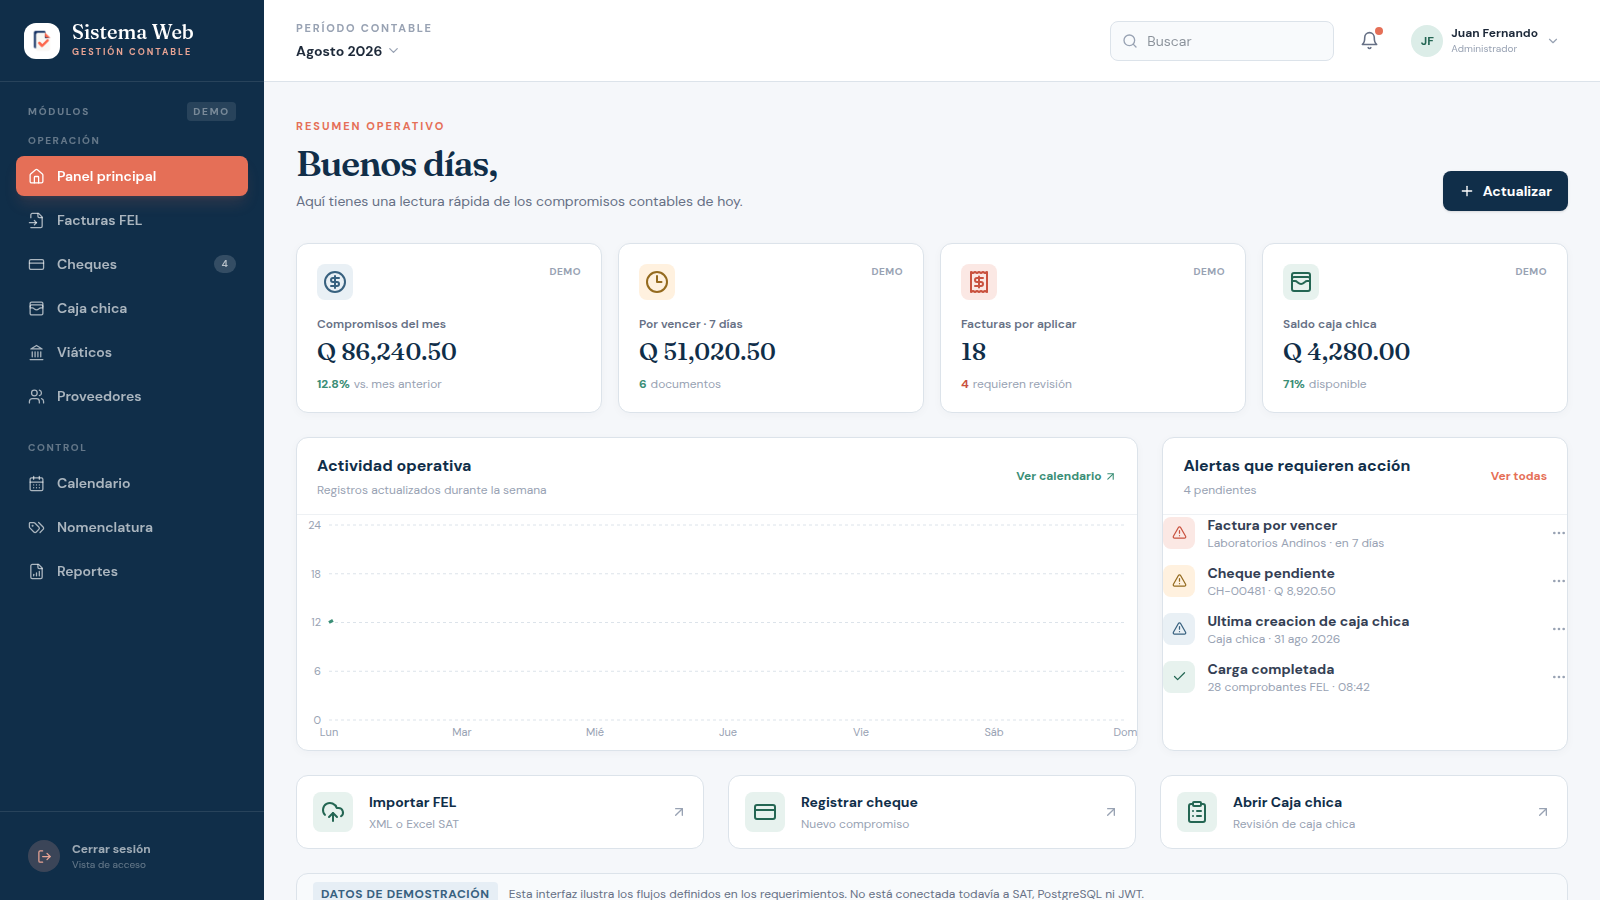
\includegraphics[width=0.96\linewidth]{imagenes/pantalla_02_dashboard.png}
\end{figure}
\begin{table}[H]\centering
\caption{Descripción de Controles del Panel Principal}
\label{tab:3_12_pantalla_dashboard}
\small\setstretch{1.15}
\begin{tabular}{p{0.25\linewidth}p{0.20\linewidth}p{0.20\linewidth}p{0.27\linewidth}}
\toprule
\textbf{Campo o control} & \textbf{Tipo} & \textbf{Valor por defecto} & \textbf{Observación} \\
\midrule
Período contable & Selector & Agosto 2026 & Define el período de consulta. \\
Buscar & Entrada & Vacío & Permite localizar información visible. \\
Indicadores & Tarjetas & Datos demostrativos & Muestran compromisos, vencimientos, facturas y saldo. \\
Alertas & Panel operativo & Pendientes & Presenta actividades que requieren atención. \\
Actualizar & Botón & Activo & Refresca la información del panel. \\
\bottomrule
\end{tabular}
\end{table}


\begin{figure}[H]
    \centering
    \caption{Módulo de Facturas FEL/SAT}
    \label{fig:pantalla_facturas}
    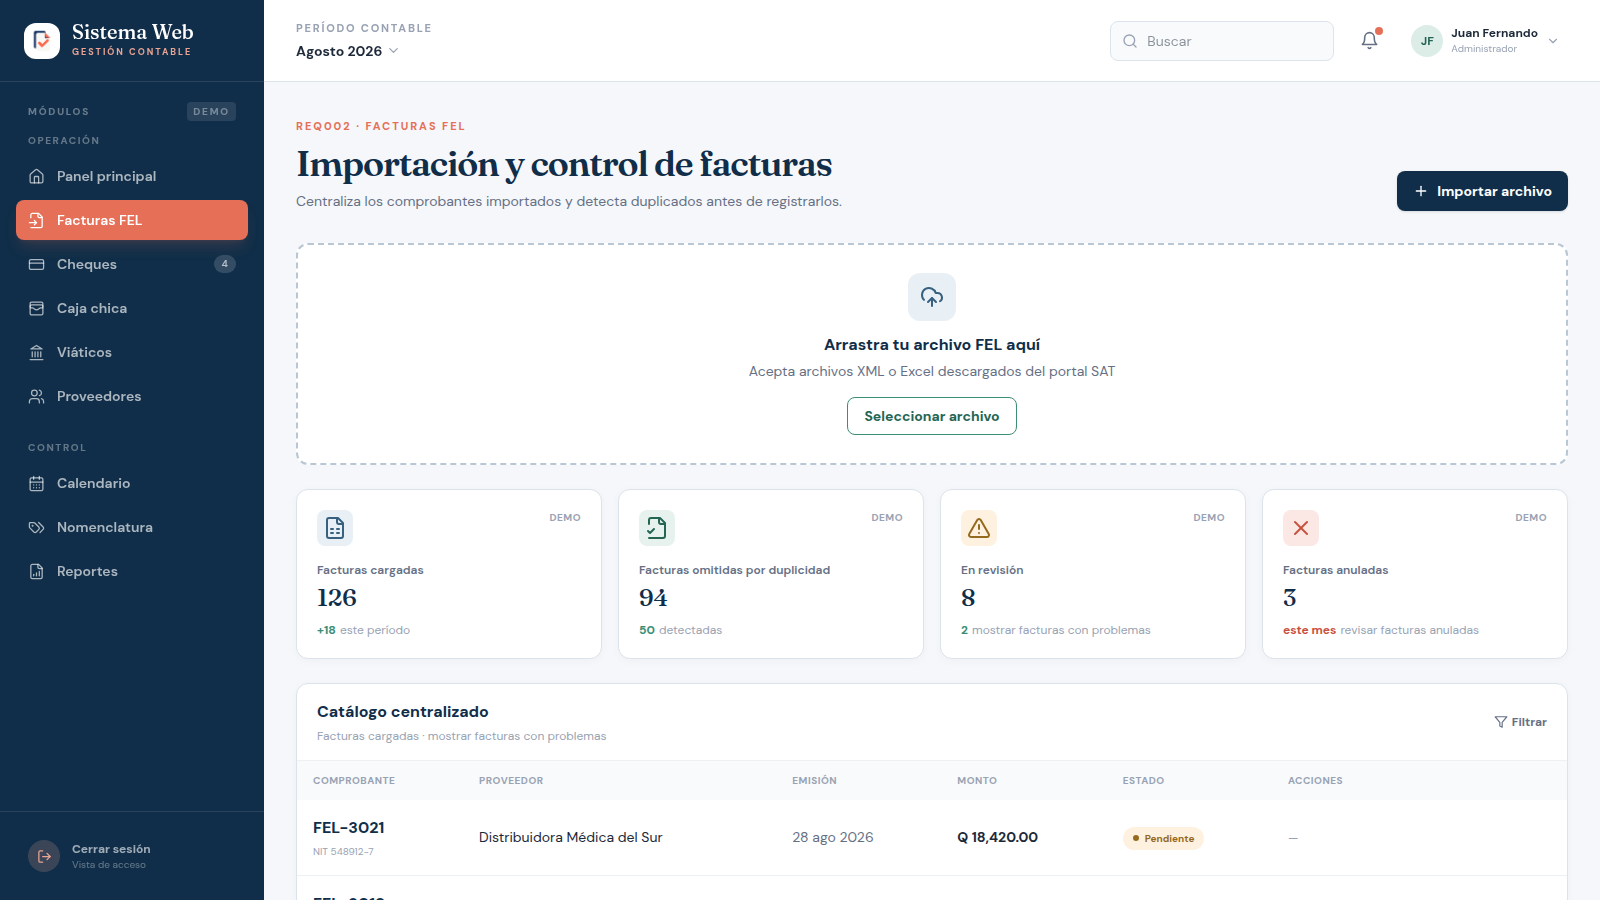
\includegraphics[width=0.96\linewidth]{imagenes/pantalla_03_facturas_fel.png}
\end{figure}
\begin{table}[H]\centering
\caption{Descripción de Controles del Módulo de Facturas FEL/SAT}
\label{tab:3_12_pantalla_facturas}
\small\setstretch{1.15}
\begin{tabular}{p{0.25\linewidth}p{0.20\linewidth}p{0.20\linewidth}p{0.27\linewidth}}
\toprule
\textbf{Campo o control} & \textbf{Tipo} & \textbf{Valor por defecto} & \textbf{Observación} \\
\midrule
Importar archivo & Botón & Activo & Inicia la carga de archivos XML o Excel. \\
Seleccionar archivo & Botón & Sin archivo & Permite elegir el archivo descargado del portal SAT. \\
Catálogo centralizado & Tabla & Registros demostrativos & Muestra comprobante, proveedor, fecha, monto y estado. \\
Editar, Aprobar y Eliminar & Acciones & Según estado & Permiten gestionar una factura autorizada. \\
Filtrar & Control & Sin filtro & Reduce los registros mostrados. \\
\bottomrule
\end{tabular}
\end{table}


\begin{figure}[H]
    \centering
    \caption{Módulo de Cheques postfechados}
    \label{fig:pantalla_cheques}
    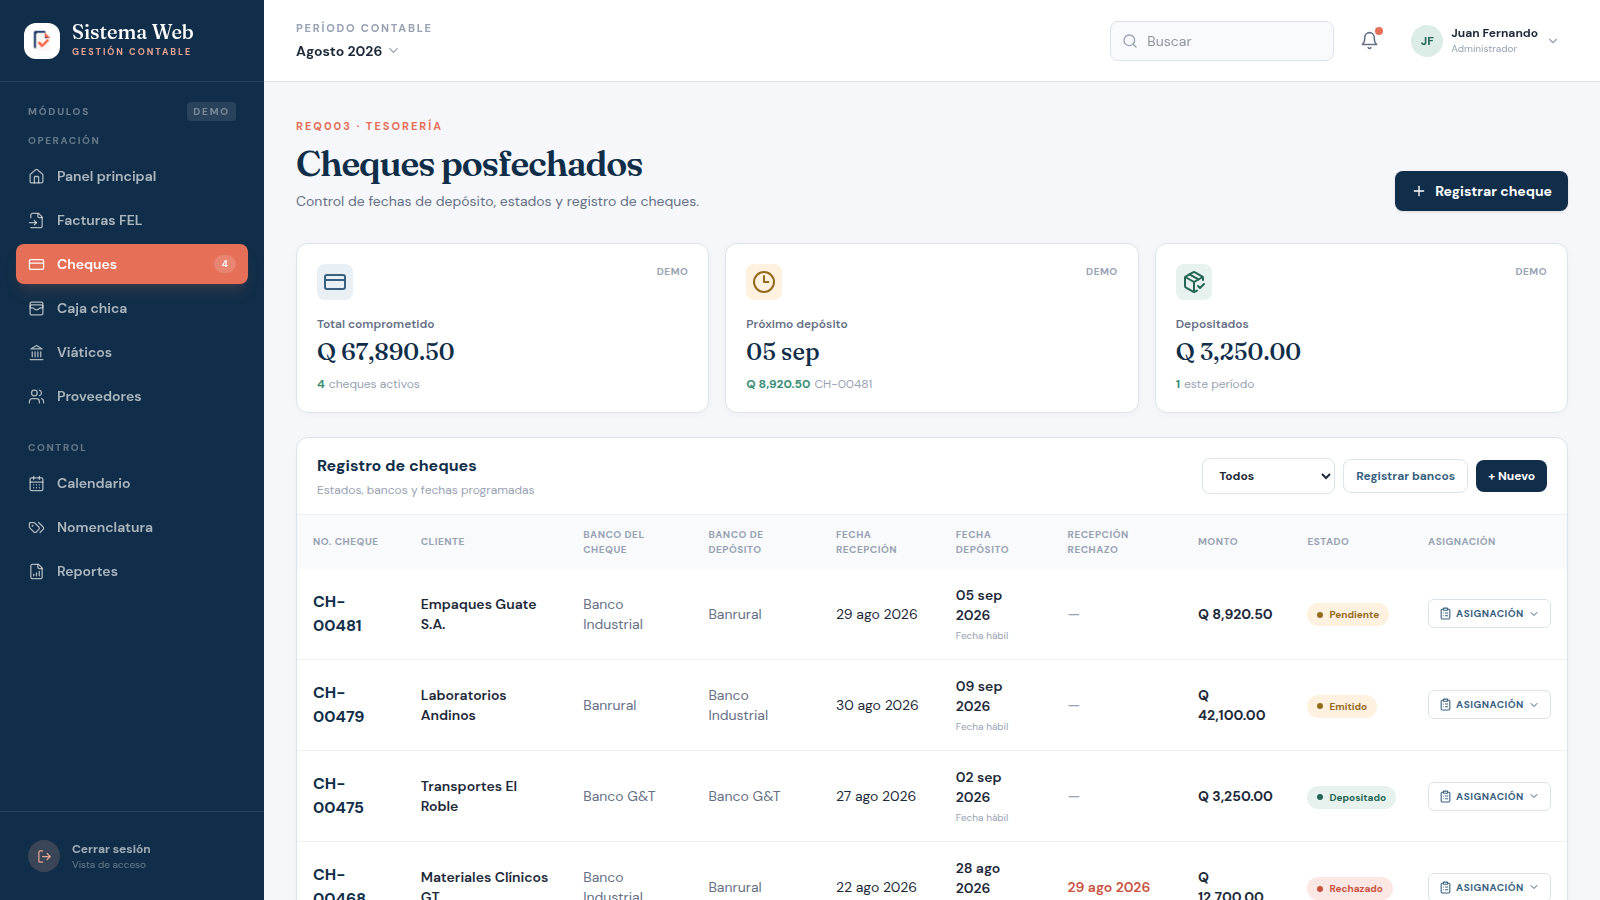
\includegraphics[width=0.96\linewidth]{imagenes/pantalla_04_cheques.png}
\end{figure}
\begin{table}[H]\centering
\caption{Descripción de Controles del Módulo de Cheques}
\label{tab:3_12_pantalla_cheques}
\small\setstretch{1.15}
\begin{tabular}{p{0.25\linewidth}p{0.20\linewidth}p{0.20\linewidth}p{0.27\linewidth}}
\toprule
\textbf{Campo o control} & \textbf{Tipo} & \textbf{Valor por defecto} & \textbf{Observación} \\
\midrule
Estado & Lista desplegable & Todos & Filtra los cheques por estado. \\
Registrar bancos & Botón & Activo & Administra bancos del cheque y de depósito. \\
Nuevo & Botón & Activo & Inicia el registro de un cheque. \\
Registro de cheques & Tabla & Registros demostrativos & Muestra cliente, bancos, fechas, monto y estado. \\
Asignación & Botón desplegable & Disponible & Muestra factura, visitador, recibo y días vencidos. \\
\bottomrule
\end{tabular}
\end{table}


\begin{figure}[H]
    \centering
    \caption{Módulo de Caja chica}
    \label{fig:pantalla_caja}
    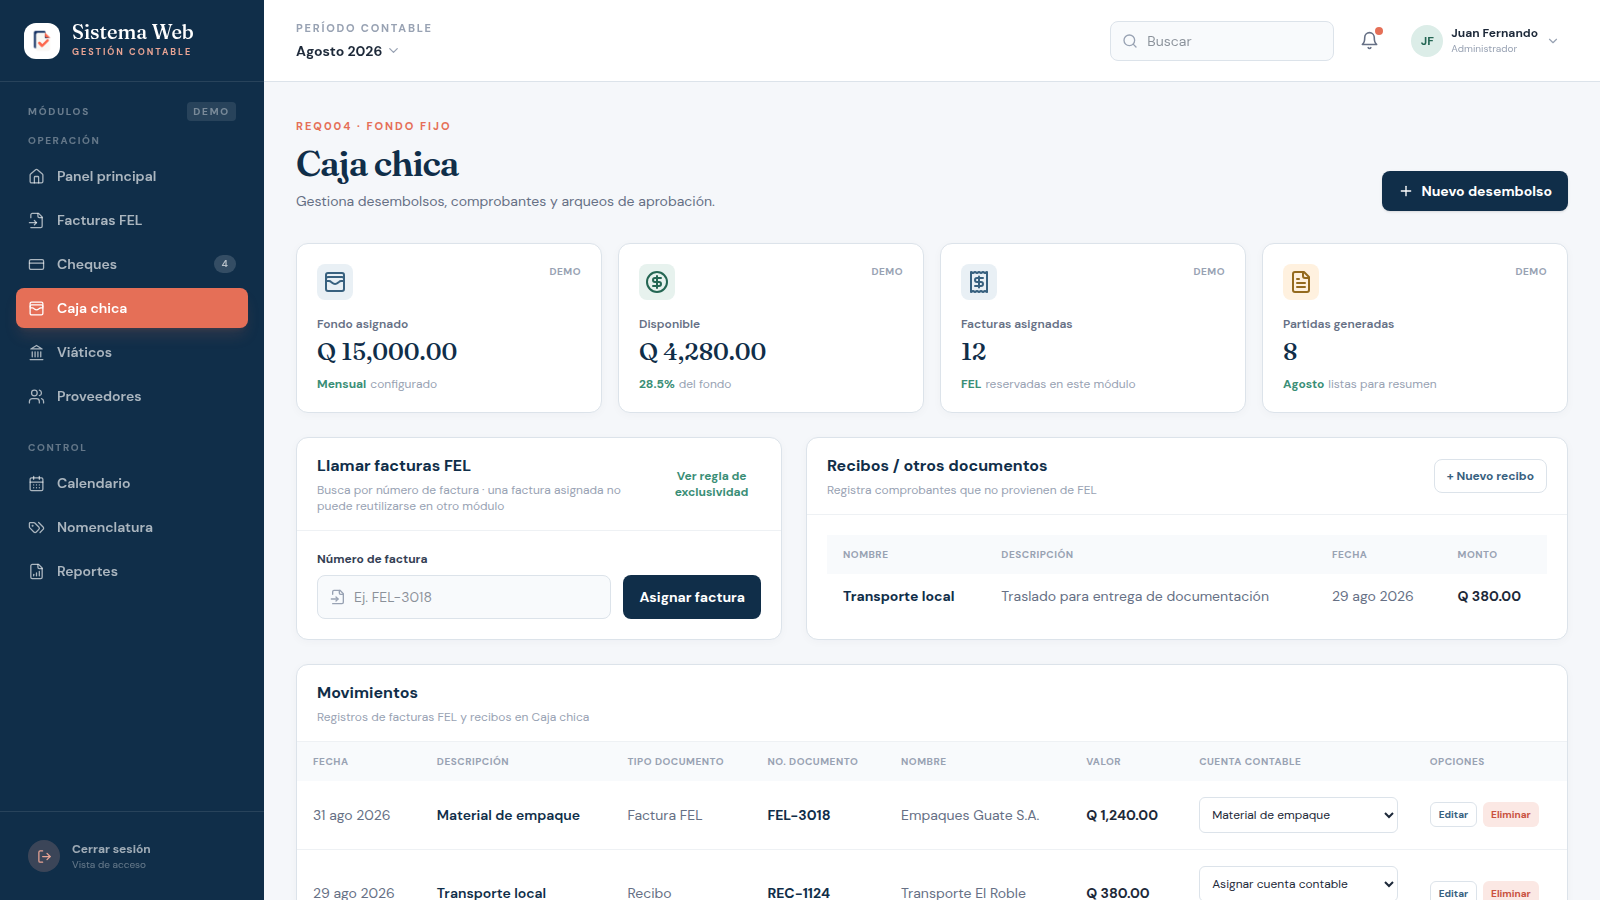
\includegraphics[width=0.96\linewidth]{imagenes/pantalla_05_caja_chica.png}
\end{figure}
\begin{table}[H]\centering
\caption{Descripción de Controles del Módulo de Caja Chica}
\label{tab:3_12_pantalla_caja}
\small\setstretch{1.15}
\begin{tabular}{p{0.25\linewidth}p{0.20\linewidth}p{0.20\linewidth}p{0.27\linewidth}}
\toprule
\textbf{Campo o control} & \textbf{Tipo} & \textbf{Valor por defecto} & \textbf{Observación} \\
\midrule
Número de factura & Entrada & Vacío & Permite llamar una factura FEL por número. \\
Asignar factura & Botón & Activo & Asigna la factura exclusivamente a Caja chica. \\
Nuevo recibo & Botón & Activo & Registra un recibo u otro documento. \\
Cuenta contable & Lista desplegable & Sugerida o manual & Permite seleccionar una cuenta de Nomenclatura. \\
Movimientos & Tabla & Registros demostrativos & Muestra fecha, descripción, documento, nombre, valor y cuenta. \\
Partida contable & Tabla & Debe y Haber & Muestra gastos, IVA y contrapartida. \\
Imprimir resumen & Botón & Activo & Abre el resumen imprimible. \\
\bottomrule
\end{tabular}
\end{table}


\begin{figure}[H]
    \centering
    \caption{Módulo de Viáticos}
    \label{fig:pantalla_viaticos}
    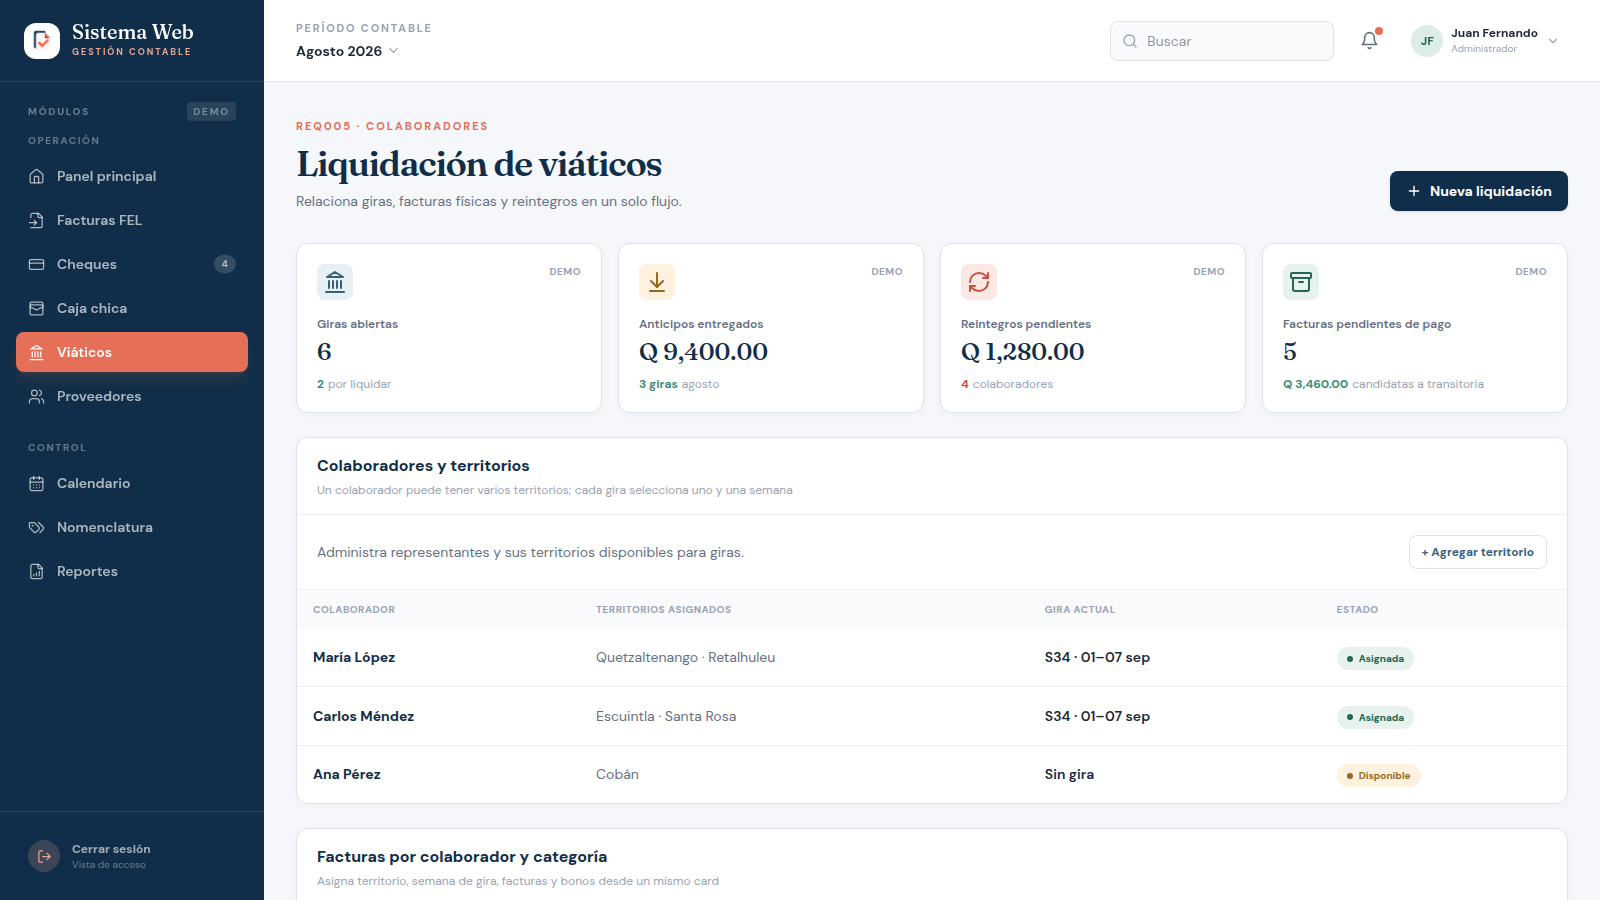
\includegraphics[width=0.96\linewidth]{imagenes/pantalla_06_viaticos.png}
\end{figure}
\begin{table}[H]\centering
\caption{Descripción de Controles del Módulo de Viáticos}
\label{tab:3_12_pantalla_viaticos}
\small\setstretch{1.15}
\begin{tabular}{p{0.25\linewidth}p{0.20\linewidth}p{0.20\linewidth}p{0.27\linewidth}}
\toprule
\textbf{Campo o control} & \textbf{Tipo} & \textbf{Valor por defecto} & \textbf{Observación} \\
\midrule
Agregar territorio & Botón & Activo & Asocia territorios disponibles a colaboradores. \\
Colaborador y gira & Lista desplegable & María López & Selecciona colaborador y territorio. \\
Semana de gira & Lista desplegable & Semana 1 & Selecciona la semana de trabajo. \\
Categoría & Lista desplegable & Viáticos & Permite elegir Viáticos, Movilidad o Actividades. \\
Bonos / otros gastos & Formulario & Vacío & Registra nombre, descripción y monto. \\
Generar partida semanal & Botón & Activo & Genera la partida de la liquidación. \\
Generar cuenta transitoria & Botón & Activo & Agrupa facturas pendientes de pago. \\
\bottomrule
\end{tabular}
\end{table}


\begin{figure}[H]
    \centering
    \caption{Pantalla de asignación de facturas}
    \label{fig:pantalla_asignacion}
    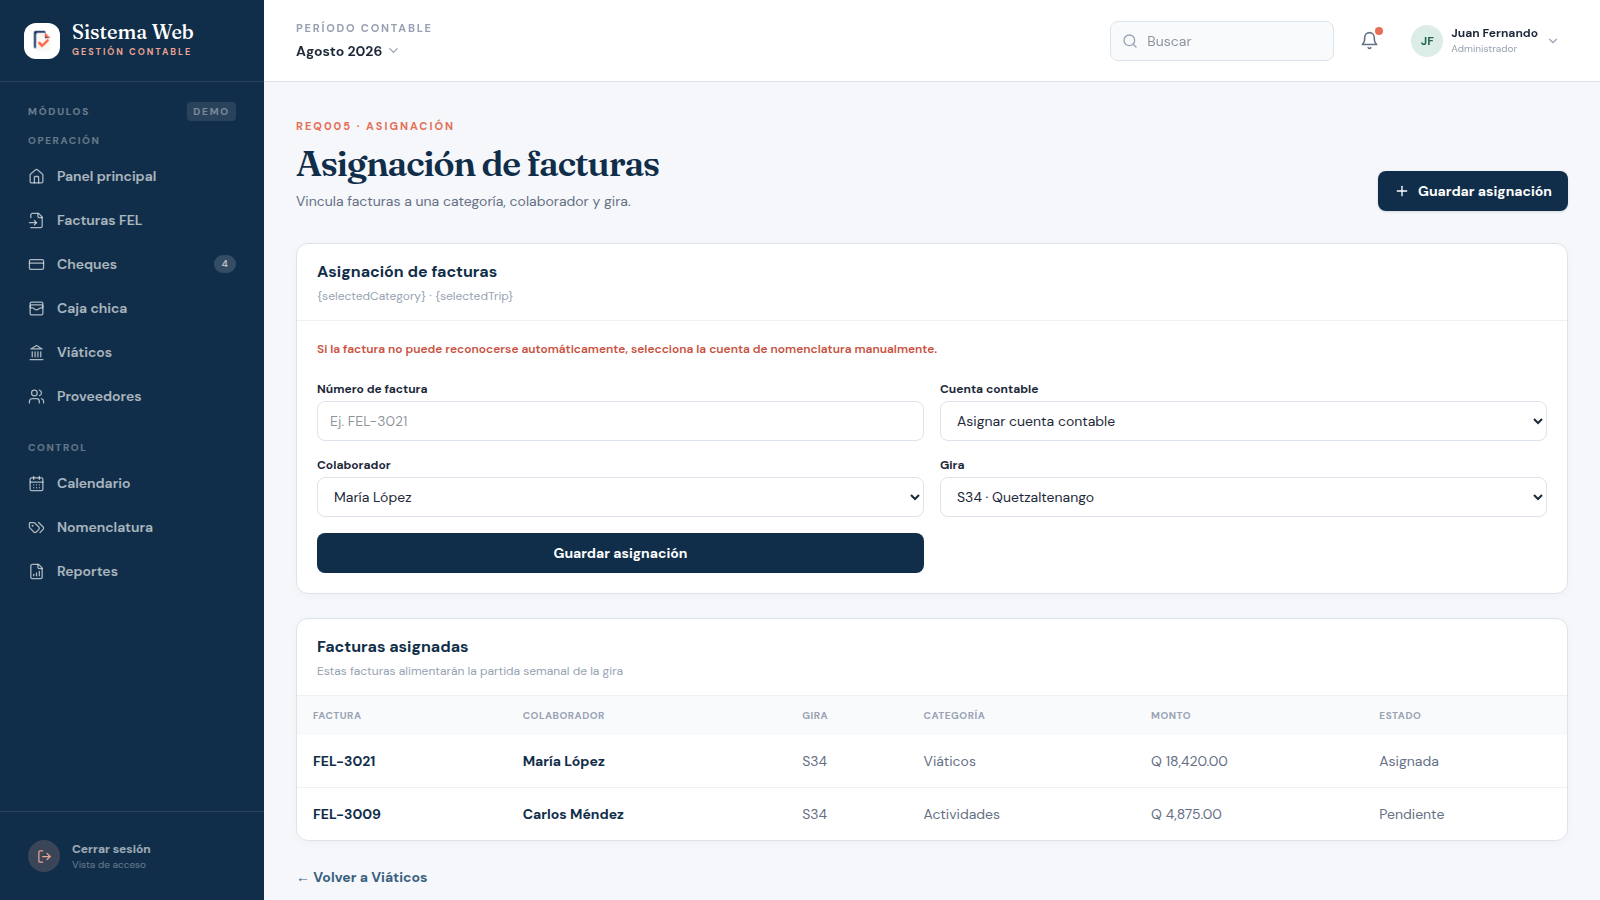
\includegraphics[width=0.96\linewidth]{imagenes/pantalla_07_asignacion_facturas.png}
\end{figure}
\begin{table}[H]\centering
\caption{Descripción de Campos de Asignación de Facturas}
\label{tab:3_12_pantalla_asignacion}
\small\setstretch{1.15}
\begin{tabular}{p{0.25\linewidth}p{0.20\linewidth}p{0.20\linewidth}p{0.27\linewidth}}
\toprule
\textbf{Campo o control} & \textbf{Tipo} & \textbf{Valor por defecto} & \textbf{Observación} \\
\midrule
Número de factura & Entrada & Vacío & Identifica el comprobante que se asignará. \\
Cuenta contable & Lista desplegable & Asignar cuenta contable & Permite seleccionar una cuenta de Nomenclatura. \\
Colaborador & Lista desplegable & María López & Asocia la factura con el colaborador. \\
Gira & Lista desplegable & S34 - Quetzaltenango & Asocia la factura con la gira. \\
Guardar asignación & Botón & Activo & Guarda la relación de factura, cuenta y gira. \\
\bottomrule
\end{tabular}
\end{table}


\begin{figure}[H]
    \centering
    \caption{Módulo de Proveedores}
    \label{fig:pantalla_proveedores}
    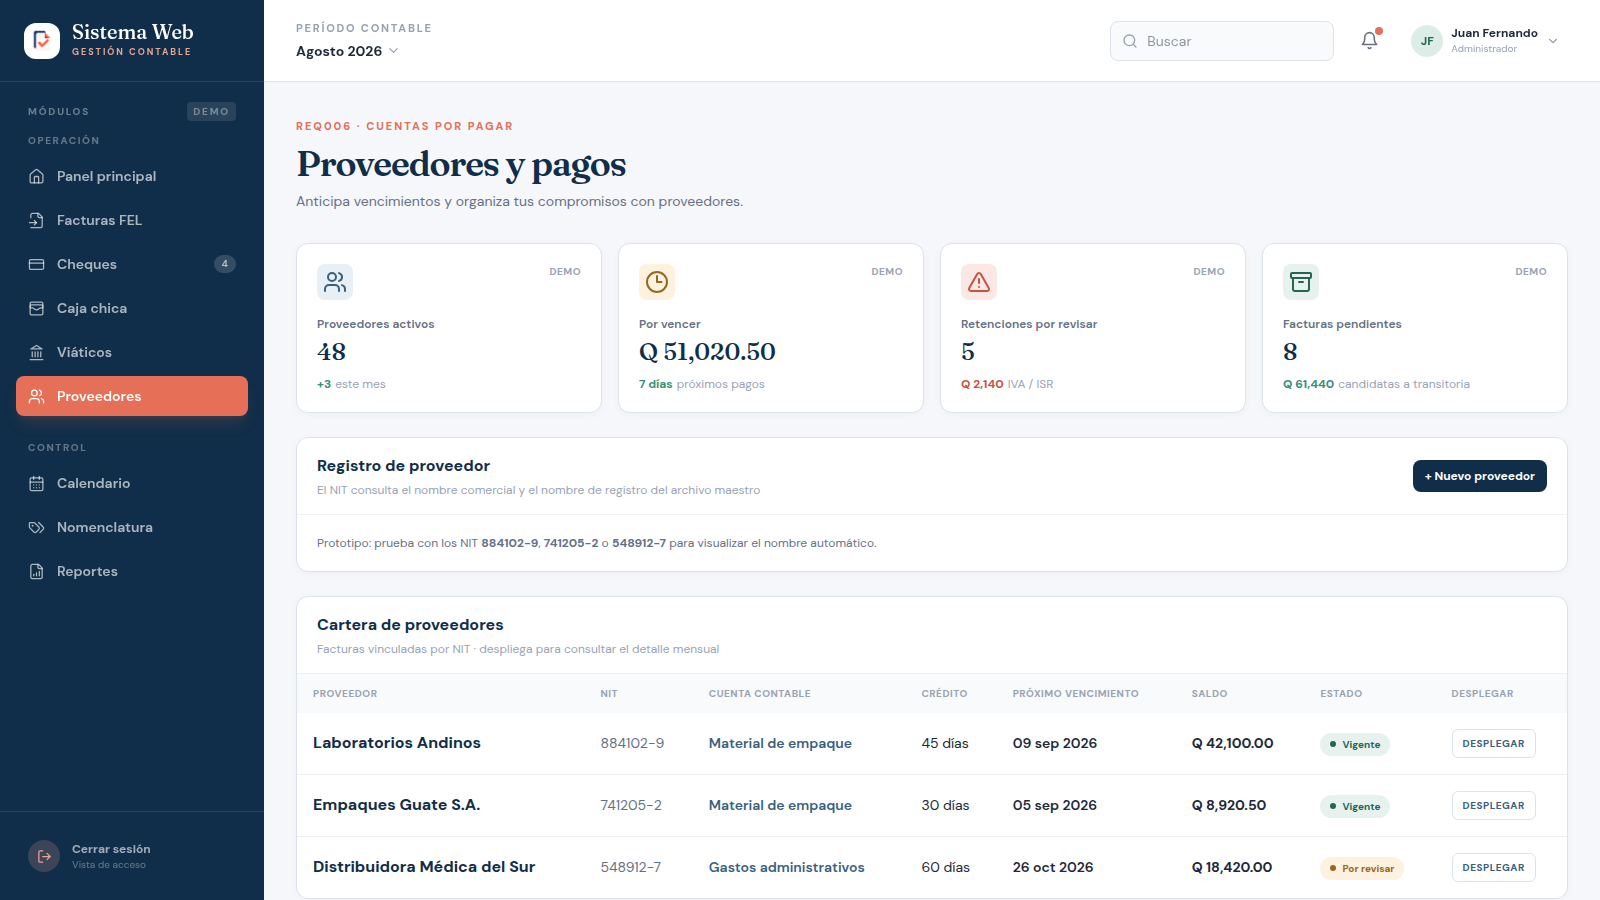
\includegraphics[width=0.96\linewidth]{imagenes/pantalla_08_proveedores.png}
\end{figure}
\begin{table}[H]\centering
\caption{Descripción de Controles del Módulo de Proveedores}
\label{tab:3_12_pantalla_proveedores}
\small\setstretch{1.15}
\begin{tabular}{p{0.25\linewidth}p{0.20\linewidth}p{0.20\linewidth}p{0.27\linewidth}}
\toprule
\textbf{Campo o control} & \textbf{Tipo} & \textbf{Valor por defecto} & \textbf{Observación} \\
\midrule
Nuevo proveedor & Botón & Activo & Inicia el registro por NIT. \\
NIT & Entrada & Vacío & Permite consultar el nombre comercial y de registro. \\
Cuenta contable & Selector & Según proveedor & Asocia la cuenta de Nomenclatura. \\
Cartera de proveedores & Tabla & Registros demostrativos & Muestra crédito, vencimiento, saldo y estado. \\
Desplegar & Botón & Disponible & Muestra las facturas mensuales del proveedor. \\
Generar partida dentro del mes & Botón & Activo & Genera la partida pagadera en el período. \\
Generar partida transitoria & Botón & Activo & Genera la partida de facturas pendientes. \\
\bottomrule
\end{tabular}
\end{table}


\begin{figure}[H]
    \centering
    \caption{Módulo de Calendario}
    \label{fig:pantalla_calendario}
    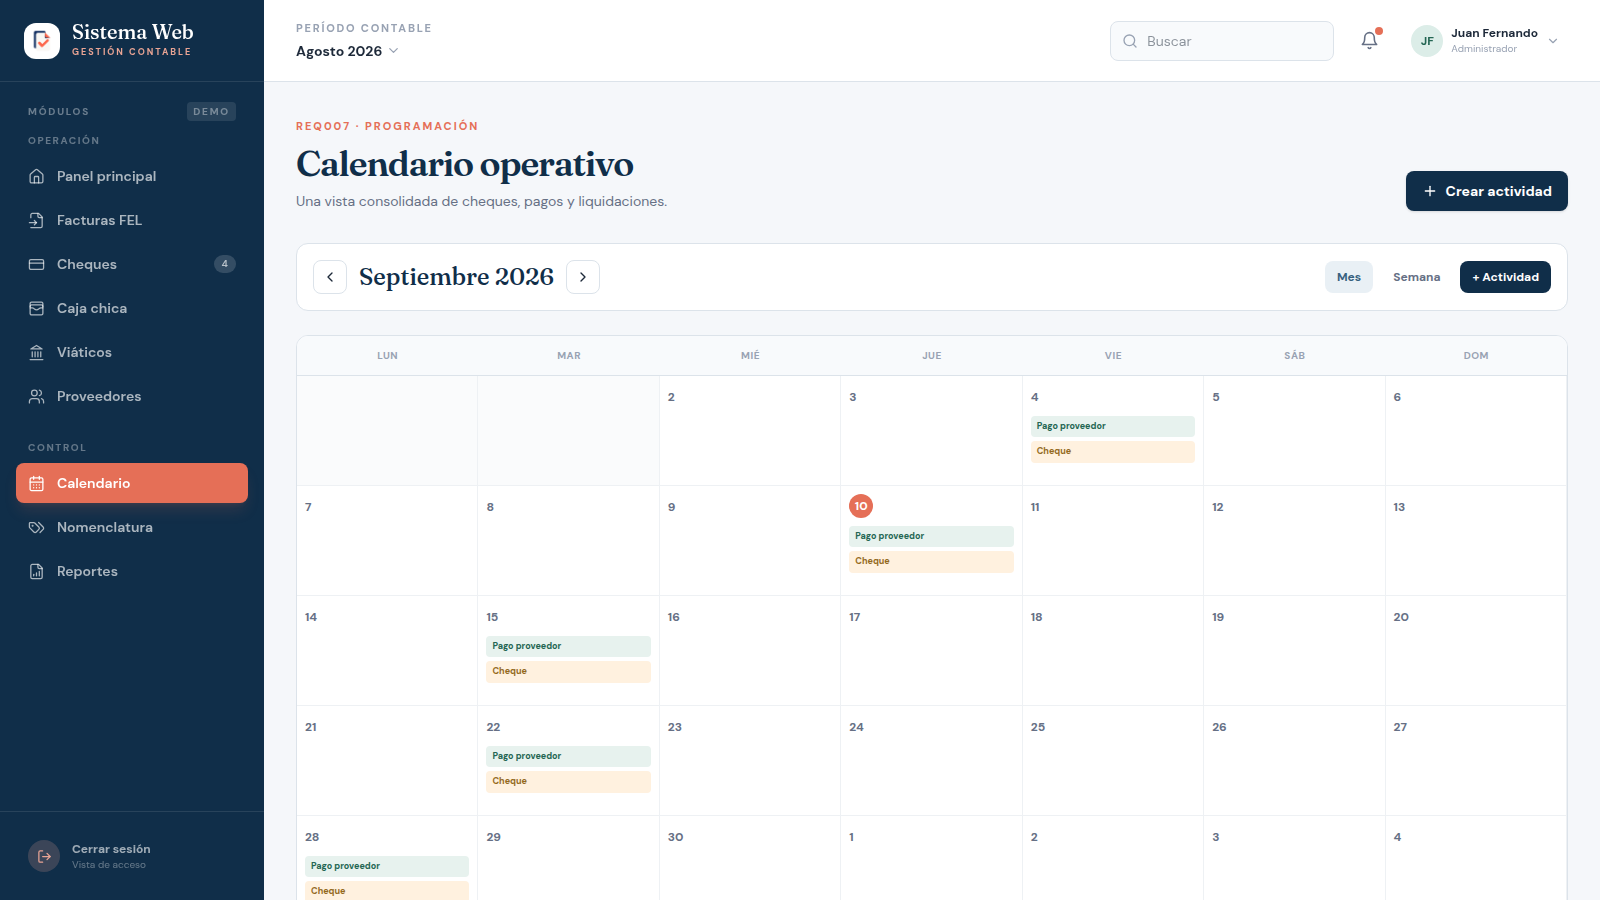
\includegraphics[width=0.96\linewidth]{imagenes/pantalla_09_calendario.png}
\end{figure}
\begin{table}[H]\centering
\caption{Descripción de Controles del Calendario Operativo}
\label{tab:3_12_pantalla_calendario}
\small\setstretch{1.15}
\begin{tabular}{p{0.25\linewidth}p{0.20\linewidth}p{0.20\linewidth}p{0.27\linewidth}}
\toprule
\textbf{Campo o control} & \textbf{Tipo} & \textbf{Valor por defecto} & \textbf{Observación} \\
\midrule
Período mensual & Navegación & Septiembre 2026 & Permite consultar el mes. \\
Anterior y siguiente & Botones & Activos & Cambian el período mostrado. \\
Mes & Selector de vista & Mes & Conserva la vista mensual. \\
Eventos & Calendario & Pagos y cheques & Presenta actividades en la fecha correspondiente. \\
Actividad & Botón & Activo & Permite registrar una actividad. \\
\bottomrule
\end{tabular}
\end{table}


\begin{figure}[H]
    \centering
    \caption{Módulo de Nomenclatura contable}
    \label{fig:pantalla_nomenclatura}
    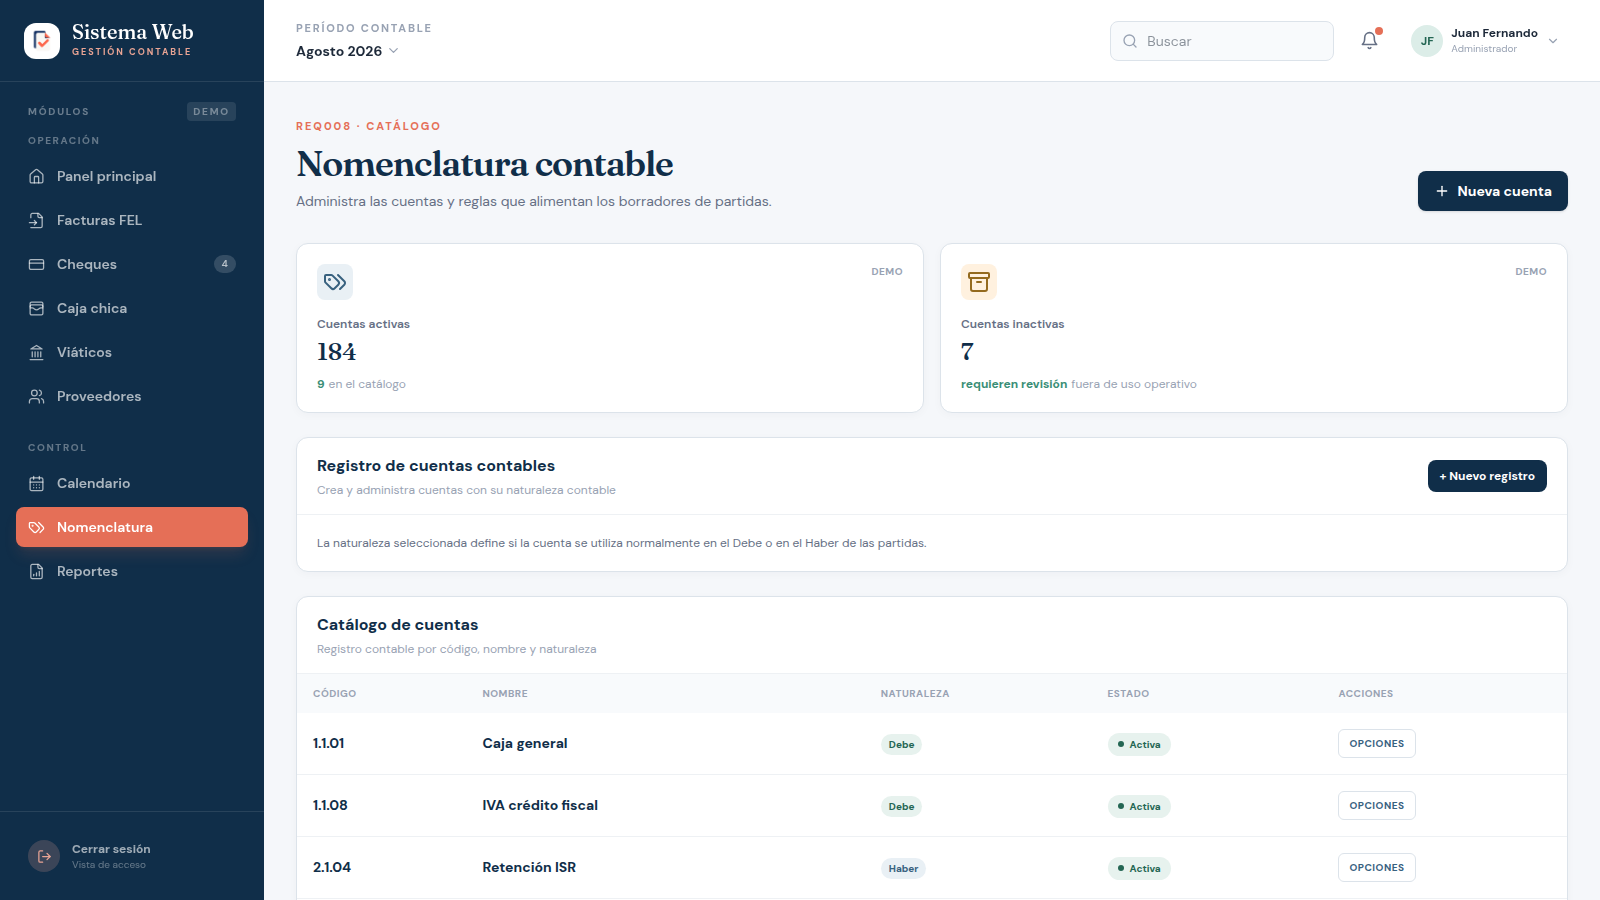
\includegraphics[width=0.96\linewidth]{imagenes/pantalla_10_nomenclatura.png}
\end{figure}
\begin{table}[H]\centering
\caption{Descripción de Controles de Nomenclatura Contable}
\label{tab:3_12_pantalla_nomenclatura}
\small\setstretch{1.15}
\begin{tabular}{p{0.25\linewidth}p{0.20\linewidth}p{0.20\linewidth}p{0.27\linewidth}}
\toprule
\textbf{Campo o control} & \textbf{Tipo} & \textbf{Valor por defecto} & \textbf{Observación} \\
\midrule
Nueva cuenta & Botón & Activo & Inicia la creación de una cuenta. \\
Nuevo registro & Botón & Activo & Abre el formulario de código, nombre y naturaleza. \\
Catálogo de cuentas & Tabla & Registros demostrativos & Muestra código, nombre, naturaleza y estado. \\
Naturaleza & Selector & Debe o Haber & Define la naturaleza contable de la cuenta. \\
Opciones & Botón & Disponible & Permite administrar cada cuenta según permisos. \\
\bottomrule
\end{tabular}
\end{table}


\begin{figure}[H]
    \centering
    \caption{Módulo de Reportes}
    \label{fig:pantalla_reportes}
    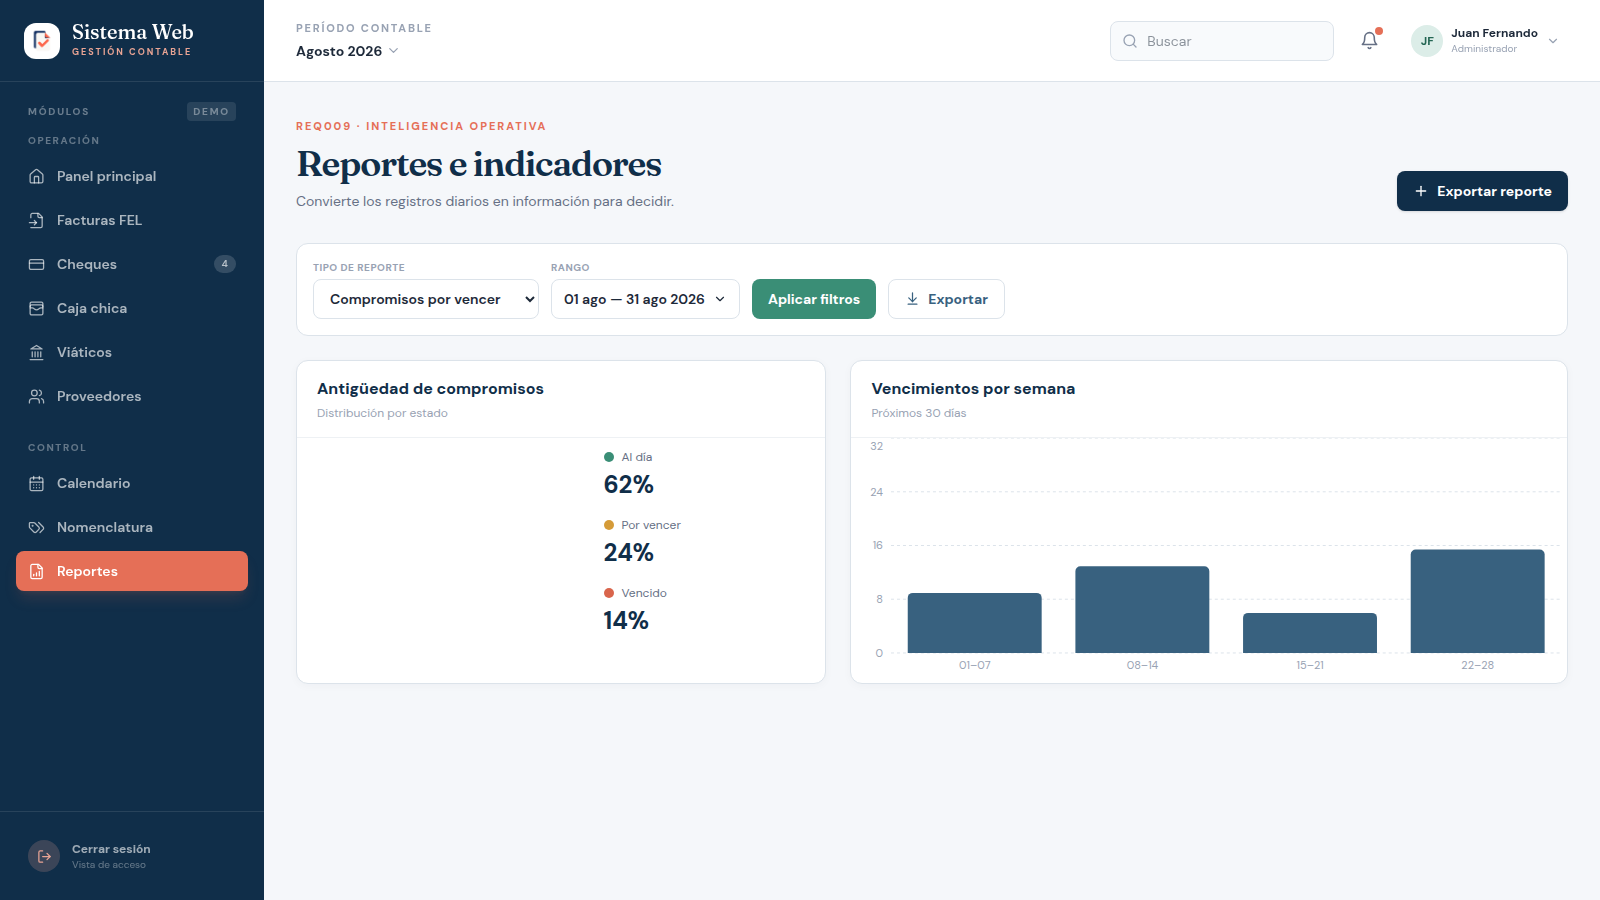
\includegraphics[width=0.96\linewidth]{imagenes/pantalla_11_reportes.png}
\end{figure}
\begin{table}[H]\centering
\caption{Descripción de Controles del Módulo de Reportes}
\label{tab:3_12_pantalla_reportes}
\small\setstretch{1.15}
\begin{tabular}{p{0.25\linewidth}p{0.20\linewidth}p{0.20\linewidth}p{0.27\linewidth}}
\toprule
\textbf{Campo o control} & \textbf{Tipo} & \textbf{Valor por defecto} & \textbf{Observación} \\
\midrule
Tipo de reporte & Lista desplegable & Compromisos por vencer & Selecciona la información que se desea analizar. \\
Rango & Lista desplegable & 01 ago - 31 ago 2026 & Define las fechas de consulta. \\
Aplicar filtros & Botón & Activo & Actualiza gráficos e indicadores. \\
Exportar & Botón & Activo & Prepara el reporte para descarga. \\
\bottomrule
\end{tabular}
\end{table}


\begin{figure}[H]
    \centering
    \caption{Resumen imprimible de Caja chica}
    \label{fig:pantalla_resumen_caja}
    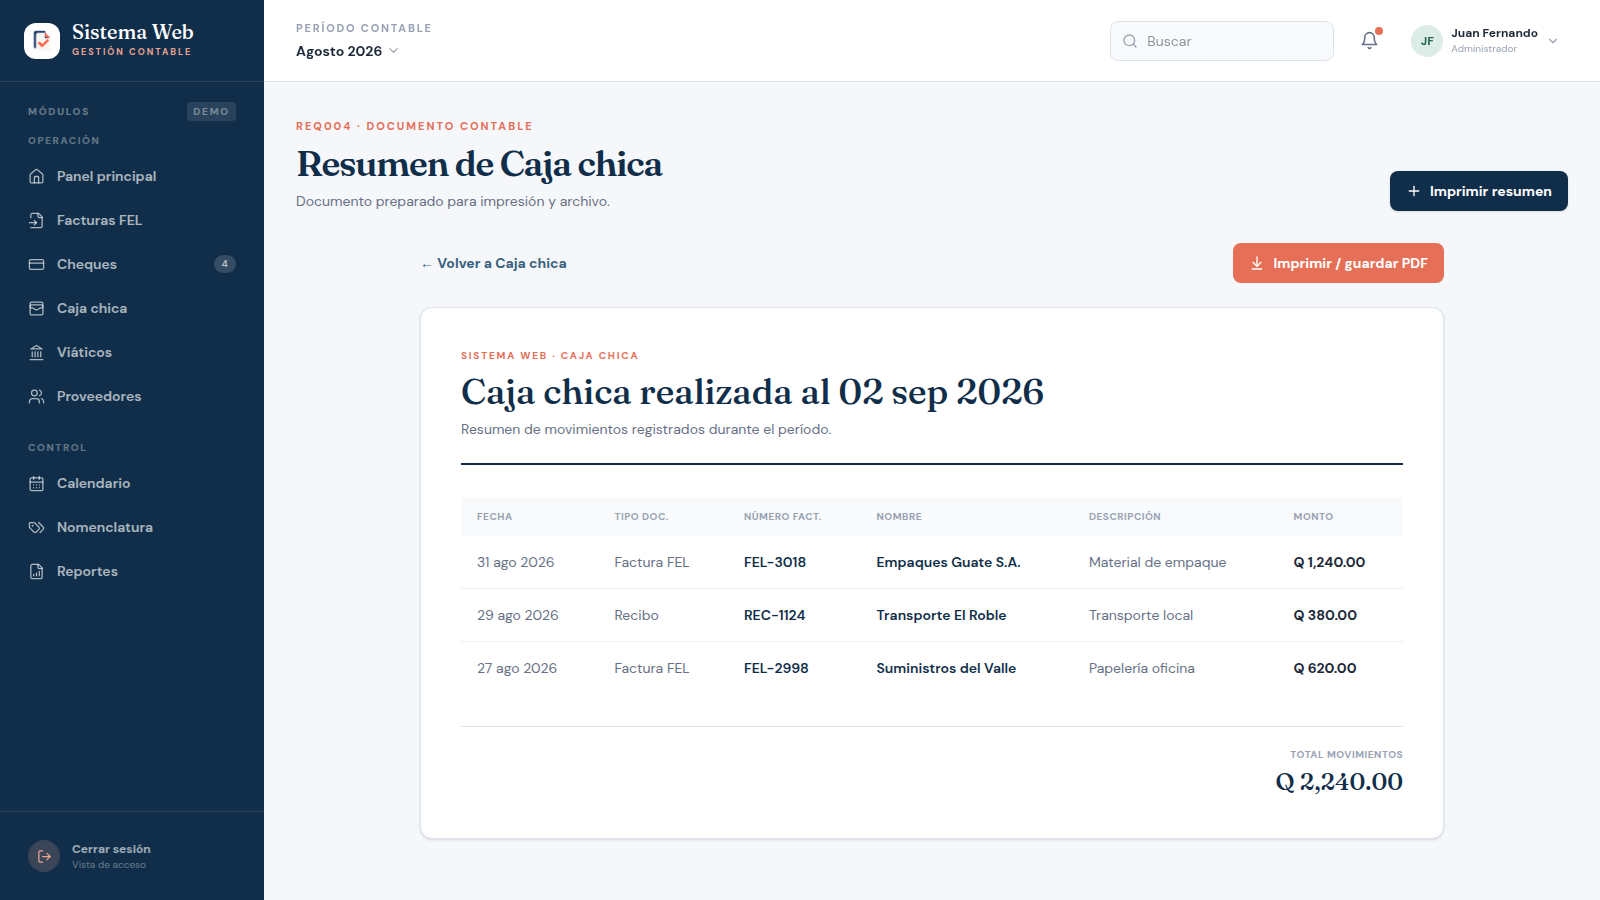
\includegraphics[width=0.96\linewidth]{imagenes/pantalla_12_resumen_caja.png}
\end{figure}
\begin{table}[H]\centering
\caption{Descripción de Controles del Resumen de Caja Chica}
\label{tab:3_12_pantalla_resumen_caja}
\small\setstretch{1.15}
\begin{tabular}{p{0.25\linewidth}p{0.20\linewidth}p{0.20\linewidth}p{0.27\linewidth}}
\toprule
\textbf{Campo o control} & \textbf{Tipo} & \textbf{Valor por defecto} & \textbf{Observación} \\
\midrule
Título y fecha & Encabezado & 02 sep 2026 & Identifica el período del resumen. \\
Imprimir / guardar PDF & Botón & Activo & Abre las opciones de impresión del navegador. \\
Detalle de movimientos & Tabla & Registros demostrativos & Incluye fecha, tipo, número, nombre, descripción y monto. \\
Total de movimientos & Total & Calculado & Permite verificar el importe antes de archivar. \\
\bottomrule
\end{tabular}
\end{table}


\subsection{Arquitectura del Sistema}

El diseño de la aplicación web propuesta se fundamenta en una arquitectura multicapa (n-tier), estructurada bajo una separación lógica de responsabilidades. Este enfoque permite aislar la presentación de la información, el procesamiento de las reglas de negocio y el almacenamiento de los datos, garantizando de esta manera la escalabilidad, el mantenimiento a largo plazo y la seguridad integral de la plataforma financiera.

La Capa de Presentación (Frontend) se desarrolla como una Aplicación de Página Única (SPA, por sus siglas en inglés) utilizando el framework Angular. Esta capa se encarga de ofrecer una interfaz gráfica intuitiva, responsiva y adaptada a las operaciones diarias del área contable. La comunicación con la Capa de Lógica de Negocio (Backend), construida bajo el lenguaje Python, se rige mediante una arquitectura API Restful. Todo el intercambio de información entre el cliente y el servidor se realiza bajo el protocolo seguro HTTPS, utilizando cargas útiles (payloads) en formato JSON y gestionando el control de acceso a través de tokens de autenticación JWT (JSON Web Tokens).

Finalmente, la Capa de Persistencia de Datos recae sobre el sistema gestor de bases de datos relacional PostgreSQL. Esta decisión garantiza el cumplimiento de las propiedades ACID (Atomicidad, Consistencia, Aislamiento y Durabilidad) y la integridad referencial de cada transacción, protegiendo así las partidas de diario y los cálculos contables. Adicionalmente, el modelo contempla un canal de integración externa (Entorno Externo) que permite la carga masiva y el análisis de archivos fiscales (Excel/XML) descargados directamente desde el portal web de la Superintendencia de Administración Tributaria (SAT).

\begin{figure}[H]
    \centering
    \caption{Arquitectura General del Sistema Propuesto}
    \label{fig:arquitectura_sistema}
    \vspace{0.2cm}
    % Se asume que la imagen está en la carpeta de imágenes
    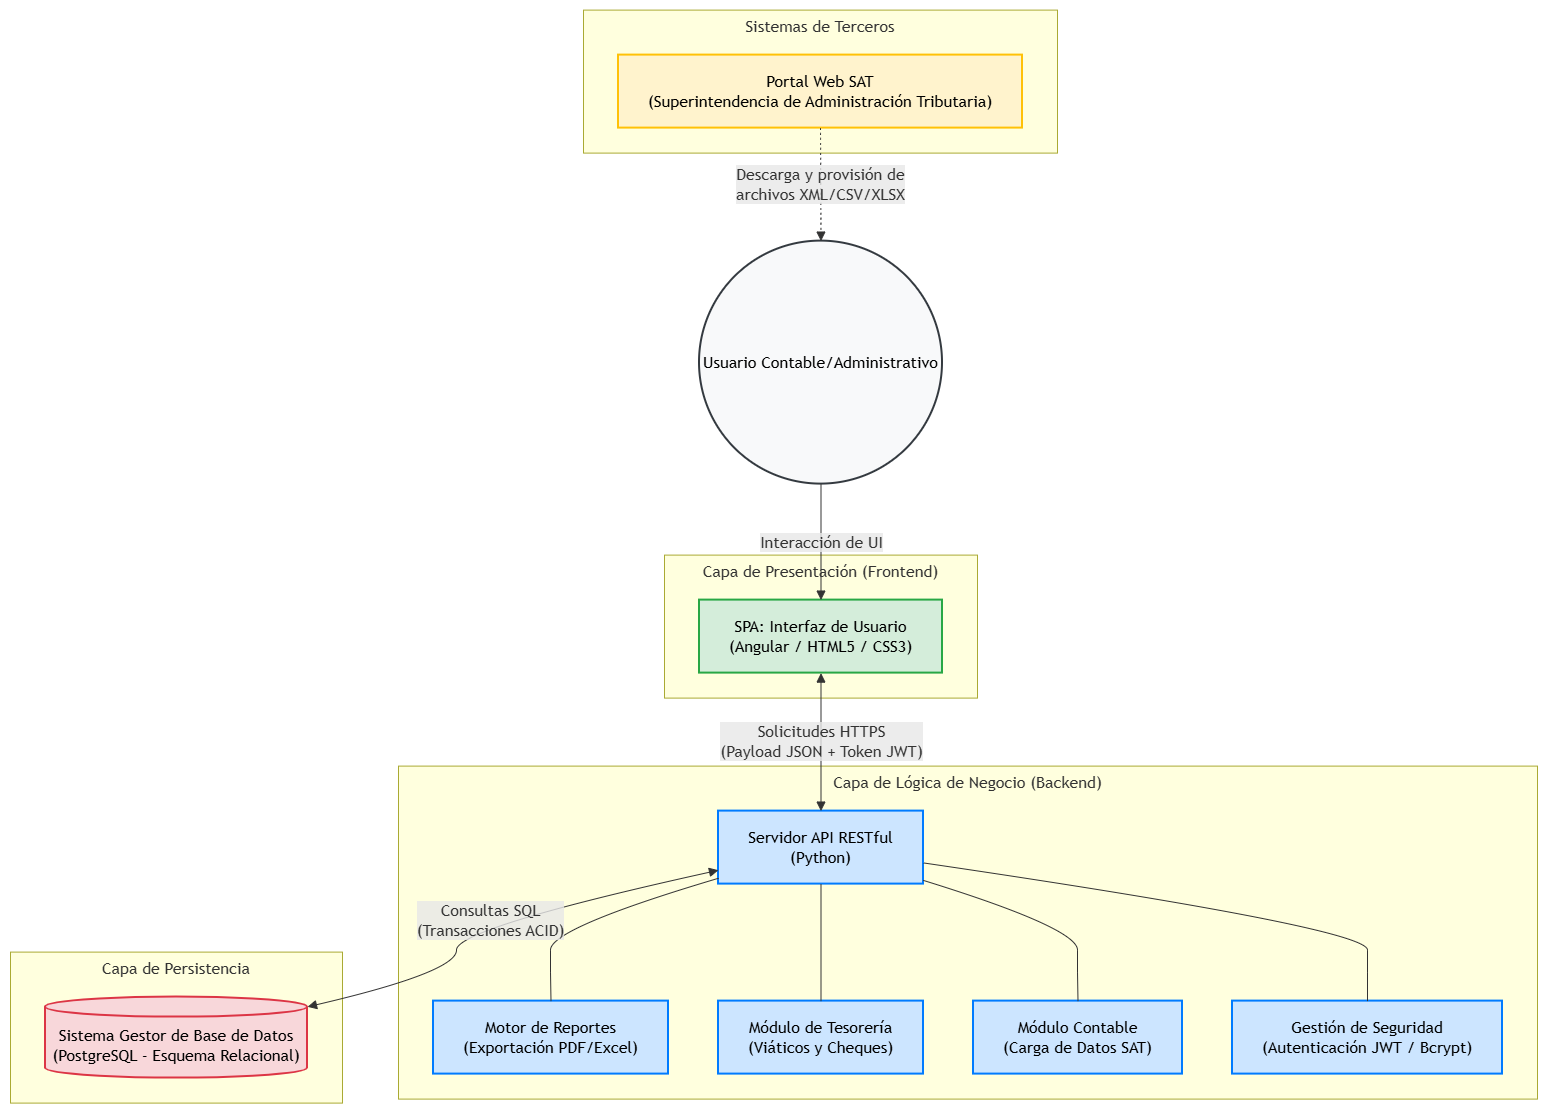
\includegraphics[width=\linewidth]{imagenes/Arquitectura.png}
\end{figure}

\subsection{Factibilidades del Proyecto}

En esta sección se describen las tecnologías y equipos que se requieren para desarrollar e implementar el software, así como la justificación del uso de cada uno. Se detallan las posibilidades y probabilidades con las que el proyecto puede ser llevado a cabo con éxito, evaluando la propuesta desde distintos enfoques técnicos, operativos, económicos, legales y ambientales.

\subsubsection{Factibilidad Técnica}

La factibilidad técnica permitió obtener la información necesaria acerca de si la tecnología requerida para implementar el sistema ya existe en el mercado, así como determinar si se cuenta con las herramientas y el software mínimos necesarios y si estos son accesibles para el desarrollo e implementación del proyecto.

{
\small
\setstretch{1.15}
\setlength{\parindent}{0pt}
\begin{xltabular}{\linewidth}{
    >{\raggedright\arraybackslash}p{4.0cm} 
    >{\raggedright\arraybackslash}p{4.0cm} 
    >{\raggedright\arraybackslash}X
}

    % --- Encabezado de la primera página ---
    \caption{Resumen de Factibilidades de Software} \label{tab:fact_software} \\
    \toprule
    \textbf{Descripción} & \textbf{Motivo} & \textbf{Herramienta Propuesta} \\
    \midrule
    \endfirsthead

    % --- Encabezado en páginas siguientes ---
    \toprule
    \textbf{Descripción} & \textbf{Motivo} & \textbf{Herramienta Propuesta} \\
    \midrule
    \endhead

    % --- Cierre en página intermedia ---
    \bottomrule
    \endfoot

    % --- Cierre final ---
    \bottomrule
    \endlastfoot

    % --- Filas de datos ---
    Lenguaje de Programación & Código fuente del sistema & Python (Backend) / TypeScript (Frontend) \\
    \addlinespace
    IDE & Entorno de desarrollo integrado & Visual Studio Code \\
    \addlinespace
    Framework & Arquitectura del software & Angular (Frontend) / FastAPI (Backend) \\
    \addlinespace
    Formularios e Interfaz & Diseño gráfico de la aplicación & Angular Material / HTML5 / CSS3 \\
    \addlinespace
    Herramienta de Reportes & Generación de documentos PDF & Librerías ReportLab / pdfkit en Python \\
    \addlinespace
    Base de Datos & Almacenamiento relacional de datos & PostgreSQL \\
    \addlinespace
    Gestor de BD & Administración de la base de datos & pgAdmin 4 \\

\end{xltabular}
}

{
\small
\setstretch{1.15}
\setlength{\parindent}{0pt}
\begin{xltabular}{\linewidth}{
    >{\raggedright\arraybackslash}p{4.0cm} 
    >{\raggedright\arraybackslash}X
}

    % --- Encabezado de la primera página ---
    \caption{Resumen de Factibilidades de Hardware} \label{tab:fact_hardware} \\
    \toprule
    \textbf{Descripción} & \textbf{Requisitos Técnicos} \\
    \midrule
    \endfirsthead

    % --- Encabezado en páginas siguientes ---
    \toprule
    \textbf{Descripción} & \textbf{Requisitos Técnicos} \\
    \midrule
    \endhead

    % --- Cierre en página intermedia ---
    \bottomrule
    \endfoot

    % --- Cierre final ---
    \bottomrule
    \endlastfoot

    % --- Filas de datos ---
    Equipo de cómputo & Computadoras con procesador Core i3 o superior, 8 GB de memoria RAM, conexión a internet y navegador web actualizado (Google Chrome o Microsoft Edge). \\
    \addlinespace
    Impresoras & Impresora láser estándar para la generación opcional de comprobantes o reportes físicos contables. \\
    \addlinespace
    Servidor & Servidor local o en la nube (AWS / DigitalOcean) con al menos 4 núcleos, 16 GB de RAM y sistema operativo Linux (Ubuntu Server). \\

\end{xltabular}
}

\subsubsection{Factibilidad Operativa}

El proyecto presenta una factibilidad operativa alta y viable para la distribuidora, sustentada en la evaluación de los siguientes aspectos clave de uso cotidiano:

\paragraph{Aceptación y Usabilidad} El sistema ha sido diseñado con una interfaz clara e intuitiva basada en estándares de Angular Material, lo que reduce significativamente la curva de aprendizaje para el personal administrativo y contable. Para garantizar una transición fluida, se entregará un manual de usuario estructurado y se impartirá una capacitación operativa previa a la puesta en marcha.

\paragraph{Alineación con los Procesos Actuales} La plataforma se integra de manera directa con los flujos de trabajo de la empresa, optimizando el tiempo de ejecución en tareas rutinarias. Al sustituir la digitación manual y las hojas de cálculo dispersas en Excel por la importación masiva de reportes de la SAT y la automatización de partidas contables, se eliminan la duplicidad de funciones y los errores humanos de cálculo sin generar conflictos operativos.

\paragraph{Gestión de la Resistencia al Cambio} La disposición del personal para adoptar la herramienta es positiva, ya que el sistema elimina la carga pesada de tabular manualmente cientos de facturas y llevar registros informales en cuadernos. Al percibir que el software actúa como un asistente que automatiza tareas repetitivas y genera alertas oportunas para pagos y depósitos, la aceptación por parte de los usuarios finales es alta.

\paragraph{Soporte y Mantenimiento Operativo} La distribuidora cuenta con el personal administrativo y contable con el perfil adecuado para la operación diaria de la plataforma. Adicionalmente, se establecerá un periodo de soporte y mantenimiento de 30 días posteriores a la entrega por parte del desarrollador para solventar cualquier eventualidad técnica, asegurando la continuidad del servicio.

\paragraph{Conclusión Operativa} Dado que el sistema satisface de manera directa las necesidades del departamento contable, facilita el trabajo cotidiano de los usuarios y cuenta con el respaldo operativo necesario, se determina que el proyecto es plenamente factible desde la perspectiva operativa.

\subsubsection{Factibilidad Económica}

La factibilidad económica evalúa la relación entre los costos involucrados en el desarrollo del sistema y los beneficios esperados de su uso. Se demuestra que las ventajas y beneficios que se obtendrán con la implementación del software superan con creces los costos asociados a su desarrollo y puesta en funcionamiento.


    \paragraph{Costos de Personal:} No se requiere la contratación de personal adicional para la fase de desarrollo o la operación diaria.
    \paragraph{Costos de Desarrollo:} El sistema es desarrollado por un estudiante de la Universidad Mariano Gálvez de Guatemala como proyecto previo a optar al título de Ingeniero en Sistemas de Información y Ciencias de la Computación, por lo que los costos de desarrollo para la empresa son nulos.
    \paragraph{Costos de Hardware:} La empresa cuenta con los equipos informáticos e infraestructura de red necesarios para operar la aplicación, por lo que no se requiere inversión en nuevo hardware.
    \paragraph{Costos de Software:} El desarrollo emplea herramientas de código abierto con licencias gratuitas, evitando gastos por adquisición de licencias comerciales.


{
\small
\setstretch{1.15}
\setlength{\parindent}{0pt}
\begin{xltabular}{\linewidth}{
    >{\raggedright\arraybackslash}p{3.5cm} 
    >{\raggedright\arraybackslash}X 
    >{\raggedright\arraybackslash}p{2.5cm}
}

    % --- Encabezado de la primera página ---
    \caption{Resumen General de los Costos Reales del Proyecto} \label{tab:costos_reales} \\
    \toprule
    \textbf{Tipo de Costo} & \textbf{Descripción} & \textbf{Valor} \\
    \midrule
    \endfirsthead

    % --- Encabezado en páginas siguientes ---
    \toprule
    \textbf{Tipo de Costo} & \textbf{Descripción} & \textbf{Valor} \\
    \midrule
    \endhead

    % --- Cierre en página intermedia ---
    \bottomrule
    \endfoot

    % --- Cierre final ---
    \bottomrule
    \endlastfoot

    % --- Filas de datos ---
    Costo de Personal & Equipo de trabajo para el desarrollo del proyecto. & Sin Costo \\
    \addlinespace
    Costos de Desarrollo & Análisis, diseño, desarrollo, implementación y pruebas del sistema. & Sin Costo \\
    \addlinespace
    Costos de Hardware & Equipo de cómputo e infraestructura de red existente. & Sin Costo \\
    \addlinespace
    Costos de Software & Licencias de código abierto (PostgreSQL, Angular, Python, FastAPI). & Sin Costo \\
    \addlinespace
    \textbf{Valor Total del Proyecto} & \textbf{Costo de desarrollo asignado al estudiante} & \textbf{Sin Costo} \\

\end{xltabular}
}

\subsubsection{Factibilidad Legal}

Esta sección evalúa el cumplimiento del proyecto respecto a las leyes y regulaciones aplicables en la República de Guatemala, asegurando que el software opere dentro del marco legal tributario, comercial y de propiedad intelectual, evitando posibles sanciones o conflictos futuros.

\paragraph{Licenciamientos de Software}
De acuerdo con la legislación guatemalteca, el software está protegido como una obra intelectual. Las herramientas seleccionadas para el desarrollo (Python, PostgreSQL, Angular y FastAPI) utilizan licencias de código abierto libres y permisivas (como la Licencia MIT), lo que faculta el uso, modificación y despliegue del sistema sin incurrir en infracciones de propiedad intelectual.

\paragraph{Régimen Legal Nacional}
El sistema respalda la validez jurídica e integridad de las operaciones y documentos digitales intercambiados dentro del módulo contable, otorgando certidumbre legal a los registros digitales de cheques, viáticos y liquidaciones de caja chica sin necesidad de trámites físicos en papel.

\paragraph{Acuerdos de Entrega del Proyecto}
El objetivo del acuerdo es entregar a la empresa el Sistema Web documentado, con sus módulos de autenticación, facturas FEL/SAT, cheques, Caja chica, Viáticos, Proveedores, Calendario, Nomenclatura y Reportes. La puesta en operación se realizará conforme al cronograma aprobado por la Universidad y a la disponibilidad operativa de la empresa.

A partir de la entrega se establece un período de 30 días de mantenimiento correctivo y acompañamiento para resolver incidencias, realizar ajustes menores y verificar la estabilidad del sistema. Cualquier ampliación posterior deberá acordarse entre la empresa y el responsable del proyecto.

\paragraph{Consideraciones tributarias y protección de datos}
El módulo FEL procesa y valida archivos XML o Excel conforme a los estándares requeridos por la Superintendencia de Administración Tributaria (SAT). El sistema aplica autenticación y control de acceso por roles para proteger la información financiera de clientes y proveedores.

\subsubsection{Factibilidad Ambiental}

A pesar de que el desarrollo e implementación de software no genera directamente desechos industriales o contaminación física severa, el proyecto ha sido concebido bajo criterios de sostenibilidad y minimización de la huella ecológica.

\paragraph{Digitalización y Reducción del Uso de Papel}
El principal impacto ambiental positivo es la eliminación paulatina de la documentación física. Al automatizar el control de cheques postfechados, la liquidación de viáticos y la conciliación de facturas FEL de la SAT, se reduce drásticamente el consumo de hojas de papel, fotocopias, carpetas e insumos de impresión.

\paragraph{Uso Eficiente de Energía y Servidores Verdes}
Para el alojamiento y despliegue de la aplicación web, se prevé la utilización de proveedores de servicios en la nube (como AWS o Google Cloud) que cuentan con políticas activas de eficiencia energética y el empleo de energías renovables en sus centros de datos.

\paragraph{Programación Ecológica (Green Software)}
Se implementaron buenas prácticas de desarrollo optimizando las consultas a la base de datos y la ejecución de código en el servidor. Esto reduce el consumo innecesario de CPU, memoria y tráfico de red, disminuyendo de manera indirecta el consumo eléctrico de los equipos de cómputo cliente que acceden a la aplicación.

\paragraph{Aprovechamiento de la Infraestructura Existente}
El sistema no requiere la adquisición de nuevos dispositivos electrónicos físicos para la empresa, fomentando la reutilización del equipo de cómputo actual y evitando la generación prematura de basura electrónica (e-waste).

\subsubsection{Análisis de Riesgos del Proyecto}

El desarrollo e implementación del sistema contable implica ciertos riesgos técnicos, operativos y de planificación. Para mitigar su impacto en el éxito del proyecto, se identifican las principales amenazas junto con su nivel de probabilidad, impacto y la estrategia de respuesta correspondiente.

{
\small
\setstretch{1.15}
\setlength{\parindent}{0pt}
\begin{xltabular}{\linewidth}{
    >{\raggedright\arraybackslash}p{2.5cm} 
    >{\raggedright\arraybackslash}p{3.5cm} 
    >{\raggedright\arraybackslash}p{1.8cm} 
    >{\raggedright\arraybackslash}p{1.8cm} 
    >{\raggedright\arraybackslash}X
}

    % --- Encabezado de la primera página ---
    \caption{Matriz de Análisis de Riesgos del Proyecto} \label{tab:analisis_riesgos} \\
    \toprule
    \textbf{Categoría} & \textbf{Riesgo Identificado} & \textbf{Probabilidad} & \textbf{Impacto} & \textbf{Estrategia de Mitigación} \\
    \midrule
    \endfirsthead

    % --- Encabezado en páginas siguientes ---
    \toprule
    \textbf{Categoría} & \textbf{Riesgo Identificado} & \textbf{Probabilidad} & \textbf{Impacto} & \textbf{Estrategia de Mitigación} \\
    \midrule
    \endhead

    % --- Cierre en página intermedia ---
    \bottomrule
    \endfoot

    % --- Cierre final ---
    \bottomrule
    \endlastfoot

    % --- Filas de datos ---
    Técnico & Cambios en la estructura de los archivos XML/Excel emitidos por la SAT. & Media & Alto & Diseñar un módulo de lectura dinámico e implementar validadores de esquemas XML flexibles con manejo claro de excepciones. \\
    \addlinespace
    Técnico & Fallas de conectividad a la base de datos PostgreSQL durante horas pico. & Baja & Alto & Implementar un pool de conexiones optimizado, índices en las tablas contables y respaldos automáticos diarios. \\
    \addlinespace
    Operativo & Resistencia del personal contable a la adopción del nuevo sistema web. & Media & Medio & Involucrar a los usuarios clave en las pruebas iniciales, elaborar un manual claro y brindar capacitaciones guiadas. \\
    \addlinespace
    Seguridad & Accesos no autorizados a la información financiera sensible. & Baja & Alto & Implementar control de acceso basado en roles (RBAC), encriptación de contraseñas y tokens JWT para la sesión de usuario. \\
    \addlinespace
    Planificación & Desfases en las fechas de entrega de los módulos según el cronograma. & Media & Medio & Aplicar el enfoque iterativo e incremental de RUP, evaluando el cumplimiento de hitos clave al finalizar cada fase (Inicio, Elaboración, Construcción y Transición). \\

\end{xltabular}
}
\subsection{Recursos del Proyecto}

Esta sección describe los componentes técnicos, físicos, lógicos y humanos necesarios para el desarrollo, despliegue y funcionamiento óptimo del sistema propuesto.

\subsubsection{Recursos de Hardware}

\paragraph{Servidores} Especificaciones de procesamiento, memoria RAM y capacidad de almacenamiento requerida (por ejemplo, servidor en la nube con 16GB de RAM y 500GB de almacenamiento SSD).

\paragraph{Estaciones de trabajo} Requisitos mínimos para los equipos de los desarrolladores y usuarios administrativos (por ejemplo, Procesador Core i5 o equivalente, 8GB de RAM).

\paragraph{Periféricos} Dispositivos físicos adicionales necesarios para la interacción con el sistema.

\subsubsection{Recursos de Software}

\paragraph{Sistemas Operativos} Plataformas sobre las cuales se ejecutará el sistema y los entornos de desarrollo (por ejemplo, Windows 10/11, distribuciones Linux, o sistemas móviles).

\paragraph{Gestores de Bases de Datos} Motor de base de datos seleccionado para el almacenamiento seguro de la información (por ejemplo, MySQL, PostgreSQL o SQL Server).

\paragraph{Lenguajes y Frameworks} Tecnologías principales utilizadas en el backend y frontend para la construcción del software.

\paragraph{Herramientas de Terceros} APIs, pasarelas de pago o librerías externas que el sistema consume para su funcionamiento.

\subsubsection{Recursos de Red y Comunicaciones}

\paragraph{Conectividad} Requisitos de ancho de banda y acceso a internet continuo para garantizar la disponibilidad del sistema alojado en la red.

\paragraph{Seguridad} Implementación de certificados SSL/TLS para el cifrado de datos en tránsito y configuración de firewalls para la protección de la infraestructura.

\subsubsection{Recursos Humanos}

\paragraph{Equipo Técnico} Roles indispensables para la creación y mantenimiento del proyecto, como desarrolladores de software, analistas de sistemas y administradores de bases de datos.

\paragraph{Usuarios del Sistema} Personal que operará la plataforma y que requerirá capacitación básica para el manejo de las interfaces.




\subsection{Cronograma de Actividades del Proyecto}

En la siguiente figura se presenta el diagrama de Gantt, el cual detalla la planificación y el tiempo estimado para cada una de las fases y actividades del proyecto.

\begin{landscape}

\begin{figure}[H]
    \centering
      \caption{Diagrama de Gantt.}
    \label{fig:diagrama_gantt}
    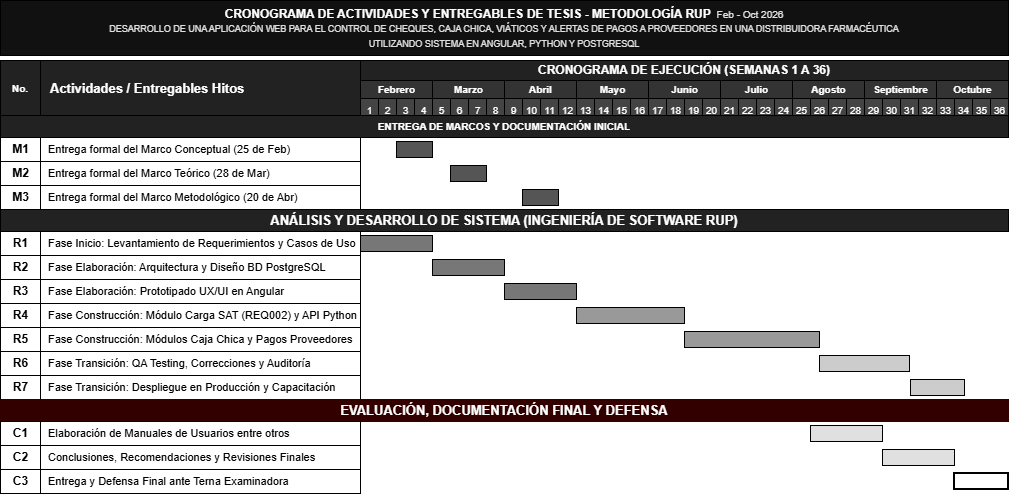
\includegraphics[width=\linewidth]{imagenes/image7.png}

\end{figure}

\end{landscape}
\section{Capítulo IV - Desarrollo de la Metodología}
\label{cap:capitulo4}

\subsection{Formularios por Módulo}
\label{sec:cap4_formularios_modulo}

El presente capítulo documenta los formularios desarrollados para el Sistema Web de gestión contable, detallando la interfaz operativa, roles de acceso, endpoints de navegación, operaciones del ciclo de vida de datos (CRUD) y las validaciones críticas implementadas en el frontend (Angular) y backend (Python/FastAPI).

% =========================================================================
% MÓDULO 1: FACTURAS FEL/SAT
% =========================================================================
\subsubsection{Módulo: Facturas FEL/SAT}

{
\small
\setstretch{1.15}
\setlength{\parindent}{0pt}
\begin{xltabular}{\linewidth}{
    >{\raggedright\arraybackslash}p{1.3cm} 
    >{\raggedright\arraybackslash}p{2.2cm} 
    >{\raggedright\arraybackslash}>{\hsize=1.15\hsize}X 
    >{\raggedright\arraybackslash}>{\hsize=0.85\hsize}X 
    >{\centering\arraybackslash}p{0.6cm} 
    >{\raggedright\arraybackslash}p{2.0cm}
}

    % --- Encabezado de la primera página ---
    \caption{Resumen de formularios - Módulo: Facturas FEL/SAT} \label{tab:cap4_fel_resumen} \\
    \toprule
    \textbf{Código} & \textbf{Formulario} & \textbf{Propósito} & \textbf{Roles/Permisos} & \textbf{Op.} & \textbf{Ruta} \\
    \midrule
    \endfirsthead

    % --- Encabezado en páginas siguientes ---
    \toprule
    \textbf{Código} & \textbf{Formulario} & \textbf{Propósito} & \textbf{Roles/Permisos} & \textbf{Op.} & \textbf{Ruta} \\
    \midrule
    \endhead

    % --- Cierre en página intermedia ---
    \bottomrule
    \endfoot

    % --- Cierre final ---
    \bottomrule
    \endlastfoot

    % --- Filas de datos ---
    F-FEL-01 & Carga Masiva FEL & Importar archivos XML/Excel autorizados por la SAT & Admin, Auxiliar ({importar\_fel}) & C & {/facturas-fel} \\
    \addlinespace
    F-FEL-02 & Catálogo FEL & Consultar, filtrar y revisar facturas importadas & Admin, Contador, Auxiliar ({ver\_fel}) & R & {/facturas-fel} \\
    \addlinespace
    F-FEL-03 & Clasificación Contable & Asignar manualmente cuenta contable a factura no identificada & Admin, Contador ({clasificar\_fel}) & U & {/facturas-fel} \\
    \addlinespace
    F-FEL-04 & Anulación / Borrado & Marcar o retirar comprobante duplicado & Admin ({eliminar\_fel}) & D & {/facturas-fel} \\

\end{xltabular}
}

\paragraph{Formulario F-FEL-01: Carga Masiva y Procesamiento FEL}
\noindent\textbf{Objetivo:} Cargar e importar comprobantes tributarios electrónicos (XML o Excel) verificando la estructura del DTE y evitando la duplicidad de registros. \\[0.3em]
\textbf{Ubicación / Ruta:} Módulo Facturas FEL $\rightarrow$ Importación ({/facturas-fel}). \\[0.3em]
\textbf{Roles/Permisos:} Admin, Auxiliar ({importar\_fel}). \\[0.3em]
\textbf{Campos clave y validaciones críticas:} {archivo\_fel} (Requerido, formatos permitidos: {.xml}, {.xlsx}, tamaño máximo: 10 MB); {uuid\_dte} (Único, requerido - extraído automáticamente, formato UUID v4); {nit\_emisor} (Requerido, formato válido SAT, ej.: {1234567-8} o {CF}); {monto\_total} (Requerido, valor mayor a cero, $>0.00$). \\[0.3em]
\textbf{Flujo:} Arrastrar o seleccionar archivo $\rightarrow$ Análisis automático de estructura $\rightarrow$ Verificación de no duplicidad por UUID $\rightarrow$ Confirmación de carga $\rightarrow$ Actualización de catálogo. \\[0.3em]
\textbf{Mensaje principal del sistema:} ``Carga completada. Se procesaron $N$ facturas FEL exitosamente.''

\begin{figure}[H]
    \centering
    \caption{Módulo de Facturas FEL/SAT con opción de importación y catálogo.}
    \label{fig:cap4_fel_pantalla}
    \vspace{0.2cm}
    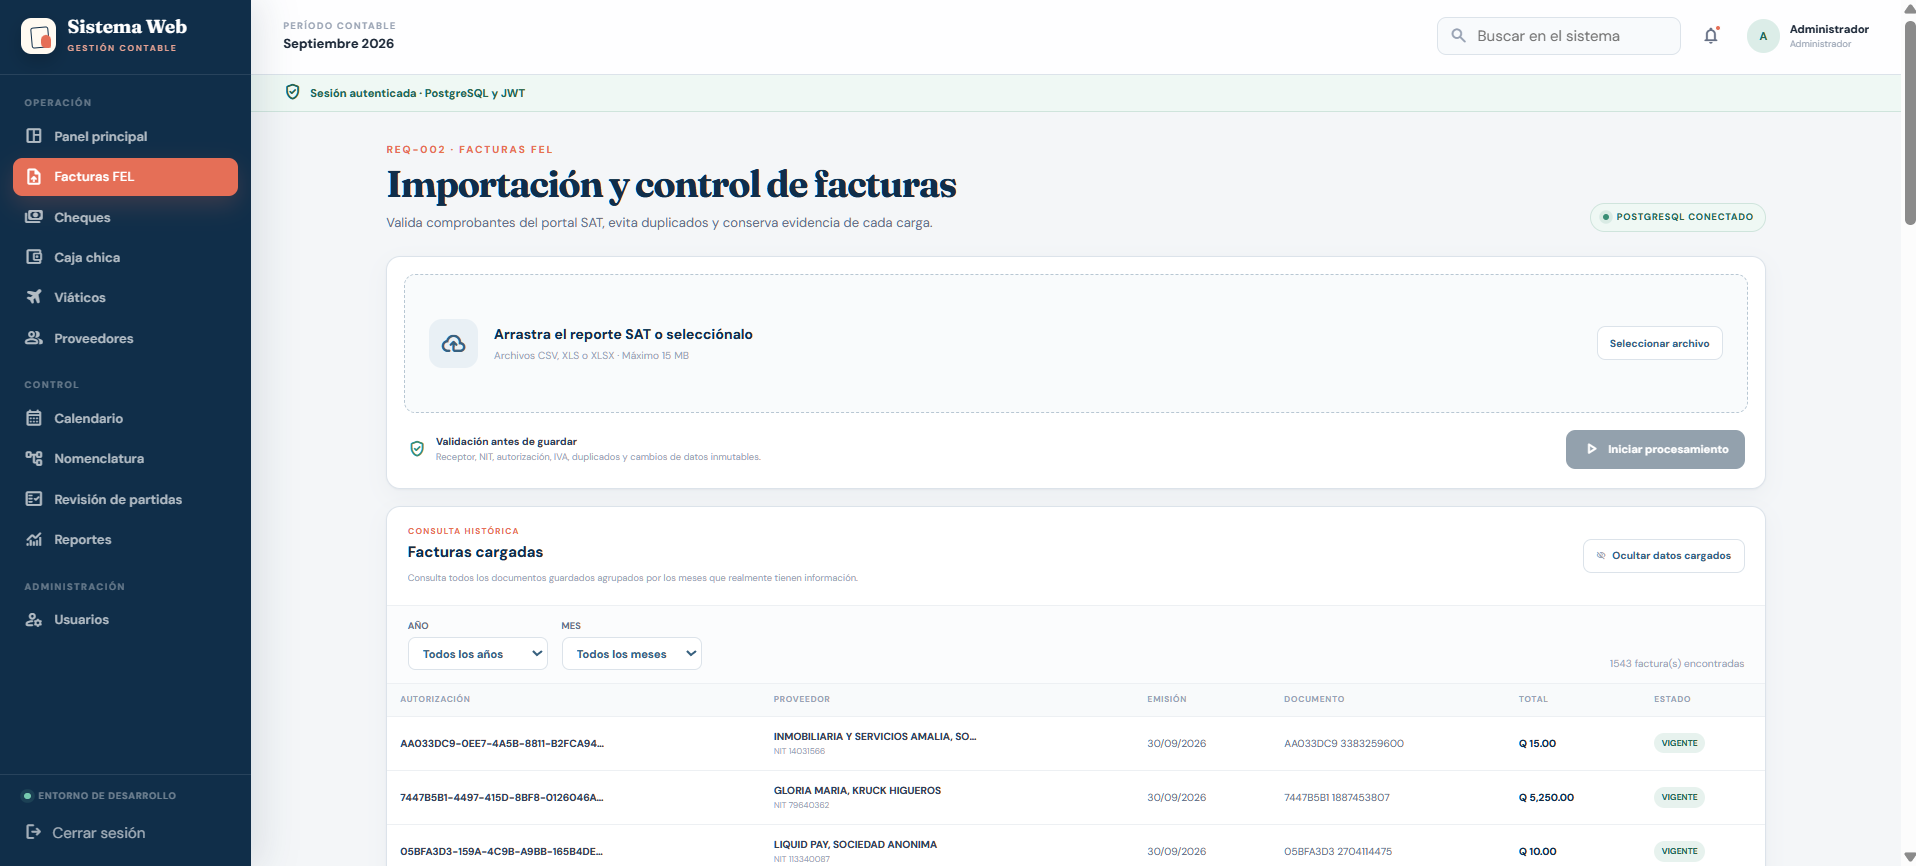
\includegraphics[width=0.96\linewidth]{capturas_reales/angular_actualizadas/pantalla_03_facturas_fel.png}
\end{figure}

% =========================================================================
% MÓDULO 2: CHEQUES POSFECHADOS
% =========================================================================
\subsubsection{Módulo: Cheques Posfechados}

{
\small
\setstretch{1.15}
\setlength{\parindent}{0pt}
\begin{xltabular}{\linewidth}{
    >{\raggedright\arraybackslash}p{1.3cm} 
    >{\raggedright\arraybackslash}p{2.2cm} 
    >{\raggedright\arraybackslash}>{\hsize=1.15\hsize}X 
    >{\raggedright\arraybackslash}>{\hsize=0.85\hsize}X 
    >{\centering\arraybackslash}p{0.6cm} 
    >{\raggedright\arraybackslash}p{2.0cm}
}

    % --- Encabezado de la primera página ---
    \caption{Resumen de formularios - Módulo: Cheques Posfechados} \label{tab:cap4_cheques_resumen} \\
    \toprule
    \textbf{Código} & \textbf{Formulario} & \textbf{Propósito} & \textbf{Roles/Permisos} & \textbf{Op.} & \textbf{Ruta} \\
    \midrule
    \endfirsthead

    % --- Encabezado en páginas siguientes ---
    \toprule
    \textbf{Código} & \textbf{Formulario} & \textbf{Propósito} & \textbf{Roles/Permisos} & \textbf{Op.} & \textbf{Ruta} \\
    \midrule
    \endhead

    % --- Cierre en página intermedia ---
    \bottomrule
    \endfoot

    % --- Cierre final ---
    \bottomrule
    \endlastfoot

    % --- Filas de datos ---
    F-CHEQ-01 & Control de Cheques & Registrar, consultar, actualizar estado y vincular a factura & Admin, Tesorero, Contador ({gestion\_cheques}) & CRUD & {/cheques} \\
    \addlinespace
    F-CHEQ-02 & Registro de Banco & Crear y administrar bancos emisores/receptores & Admin ({crear\_bancos}) & C & {/cheques} \\

\end{xltabular}
}

\paragraph{Formulario F-CHEQ-01: Gestión Integrada de Cheques Posfechados}
\noindent\textbf{Objetivo:} Registrar cheques de clientes, asociar banco receptor, dar seguimiento a fechas de depósito y vincular el pago a facturas emitidas. \\[0.3em]
\textbf{Ubicación / Ruta:} Módulo Cheques $\rightarrow$ Control de Cheques ({/cheques}). \\[0.3em]
\textbf{Roles/Permisos:} Admin, Tesorero, Contador ({gestion\_cheques}). \\[0.3em]
\textbf{Campos clave y validaciones críticas:} {numero\_cheque} (Requerido, numérico o alfanumérico único por banco, ej.: {CHQ-99482}); {cliente} (Requerido, texto o selección de catálogo); {banco\_origen} y {banco\_deposito} (Seleccionados de catálogo activo); {fecha\_recepcion} y {fecha\_deposito} (Requeridas, {fecha\_deposito} $\ge$ {fecha\_recepcion}); {monto} (Requerido, numérico mayor a cero, $>0.00$); {estado} (Requerido: Pendiente, Depositado, Rechazado). \\[0.3em]
\textbf{Flujo:} Hacer clic en ``Nuevo'' $\rightarrow$ Completar datos del cheque $\rightarrow$ Seleccionar factura o recibo en ``Asignación'' $\rightarrow$ Guardar registro. \\[0.3em]
\textbf{Mensaje principal del sistema:} ``Cheque registrado correctamente No. CHQ-99482.''

\begin{figure}[H]
    \centering
    \caption{Formulario y control de cheques posfechados anotado.}
    \label{fig:cap4_cheques_pantalla}
    \vspace{0.2cm}
    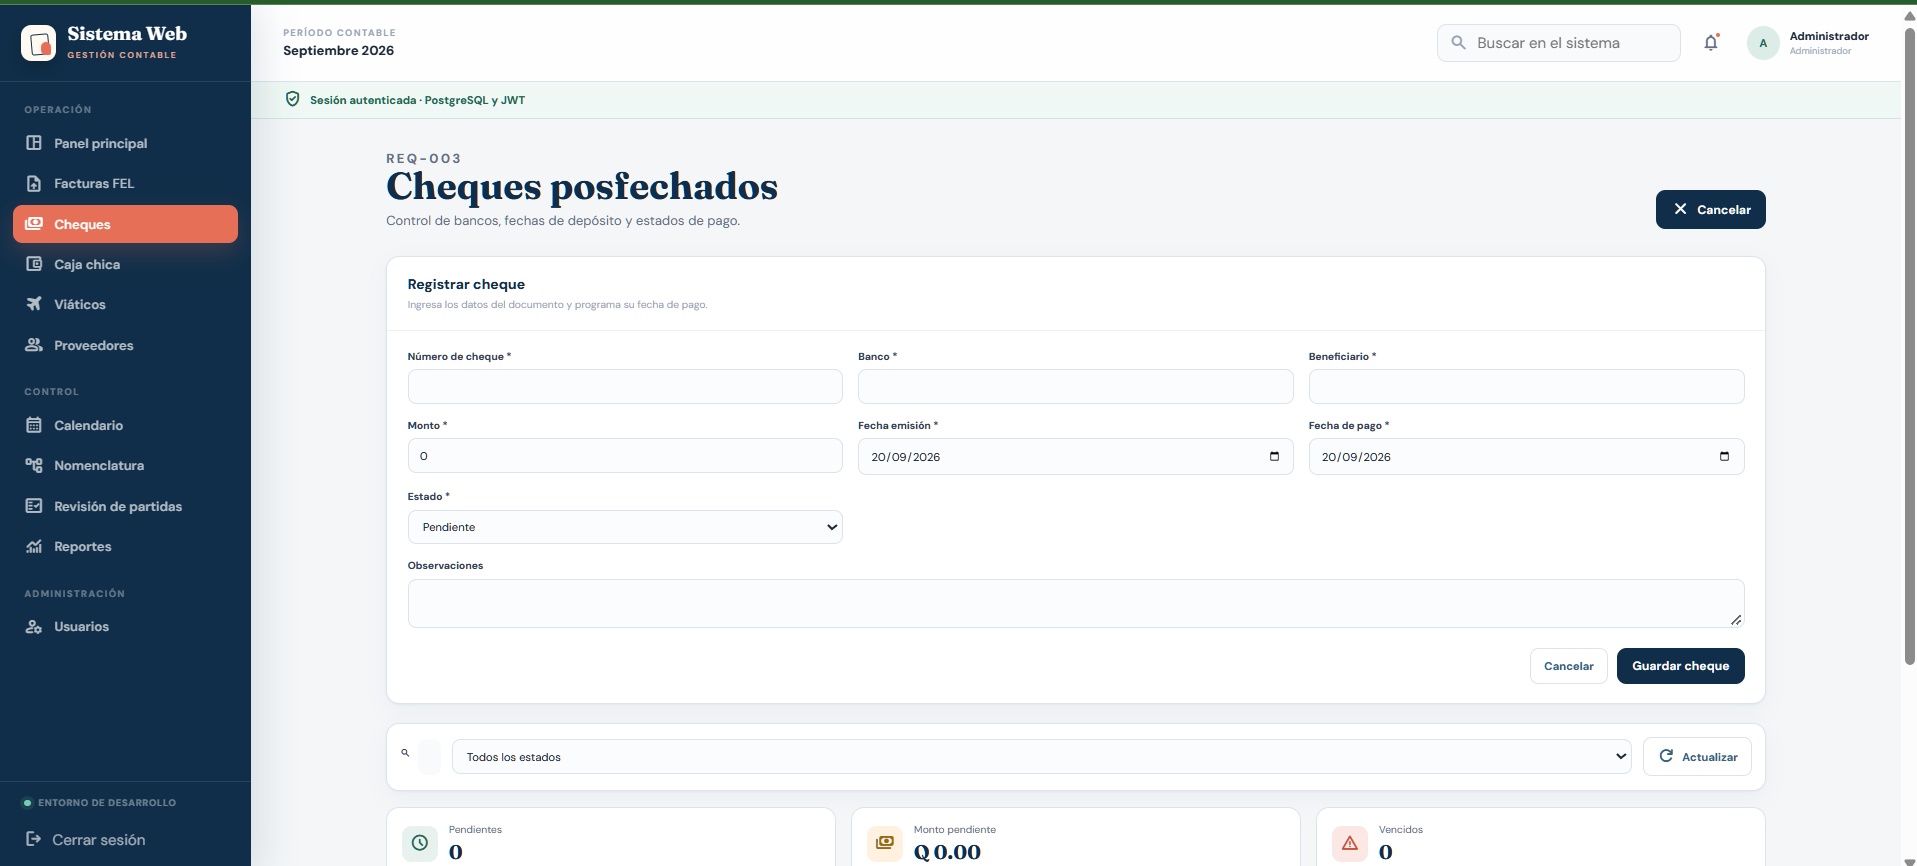
\includegraphics[width=0.96\linewidth]{capturas_reales/angular_actualizadas/formulario_cheque.png}
\end{figure}

% =========================================================================
% MÓDULO 3: CAJA CHICA
% =========================================================================
\subsubsection{Módulo: Caja Chica}

{
\small
\setstretch{1.15}
\setlength{\parindent}{0pt}
\begin{xltabular}{\linewidth}{
    >{\raggedright\arraybackslash}p{1.3cm} 
    >{\raggedright\arraybackslash}p{2.2cm} 
    >{\raggedright\arraybackslash}>{\hsize=1.15\hsize}X 
    >{\raggedright\arraybackslash}>{\hsize=0.85\hsize}X 
    >{\centering\arraybackslash}p{0.6cm} 
    >{\raggedright\arraybackslash}p{2.0cm}
}

    % --- Encabezado de la primera página ---
    \caption{Resumen de formularios - Módulo: Caja Chica} \label{tab:cap4_cajachica_resumen} \\
    \toprule
    \textbf{Código} & \textbf{Formulario} & \textbf{Propósito} & \textbf{Roles/Permisos} & \textbf{Op.} & \textbf{Ruta} \\
    \midrule
    \endfirsthead

    % --- Encabezado en páginas siguientes ---
    \toprule
    \textbf{Código} & \textbf{Formulario} & \textbf{Propósito} & \textbf{Roles/Permisos} & \textbf{Op.} & \textbf{Ruta} \\
    \midrule
    \endhead

    % --- Cierre en página intermedia ---
    \bottomrule
    \endfoot

    % --- Cierre final ---
    \bottomrule
    \endlastfoot

    % --- Filas de datos ---
    F-CAJA-01 & Asignar Factura FEL & Vincular factura FEL al fondo de Caja Chica & Admin, Operativo ({caja\_asigna\_fel}) & C & {/caja-chica} \\
    \addlinespace
    F-CAJA-02 & Nuevo Recibo & Registrar egreso de fondo sin comprobante FEL & Admin, Operativo ({caja\_recibos}) & C & {/caja-chica} \\
    \addlinespace
    F-CAJA-03 & Generación Partida & Crear asiento contable de liquidación y arqueo & Admin, Contador ({caja\_partidas}) & C/U & {/caja-chica} \\
    \addlinespace
    F-CAJA-04 & Resumen de Fondo & Visualización e impresión de arqueo del período & Admin, Contador, Auxiliar ({caja\_resumen}) & R & {/caja-chica} \\

\end{xltabular}
}

\paragraph{Formulario F-CAJA-02: Registro de Recibo / Egreso de Caja Chica}
\noindent\textbf{Objetivo:} Registrar egresos del fondo fijo respaldados por vales o recibos internos, sugiriendo o clasificando la cuenta contable de gasto. \\[0.3em]
\textbf{Ubicación / Ruta:} Módulo Caja Chica $\rightarrow$ Nuevo Recibo ({/caja-chica}). \\[0.3em]
\textbf{Roles/Permisos:} Admin, Operativo ({caja\_recibos}). \\[0.3em]
\textbf{Campos clave y validaciones críticas:} {fecha\_movimiento} (Requerida, dentro del período contable activo); {tipo\_documento} (Requerido: Recibo, Vale, Factura Exenta); {numero\_documento} (Requerido, ej.: {REC-00124}); {nombre\_beneficiario} (Requerido); {monto\_total} (Requerido, no puede exceder el fondo disponible, $>0.00$); {cuenta\_contable} (Requerida, seleccionada de Nomenclatura). \\[0.3em]
\textbf{Flujo:} Presionar ``Nuevo recibo'' $\rightarrow$ Capturar datos y monto $\rightarrow$ Asignar o validar cuenta contable de Nomenclatura $\rightarrow$ Guardar registro $\rightarrow$ Actualizar saldo del fondo. \\[0.3em]
\textbf{Mensaje principal del sistema:} ``Movimiento de Caja Chica registrado exitosamente.''

\begin{figure}[H]
    \centering
    \caption{Módulo de Caja Chica con captura de recibos y liquidación.}
    \label{fig:cap4_cajachica_pantalla}
    \vspace{0.2cm}
    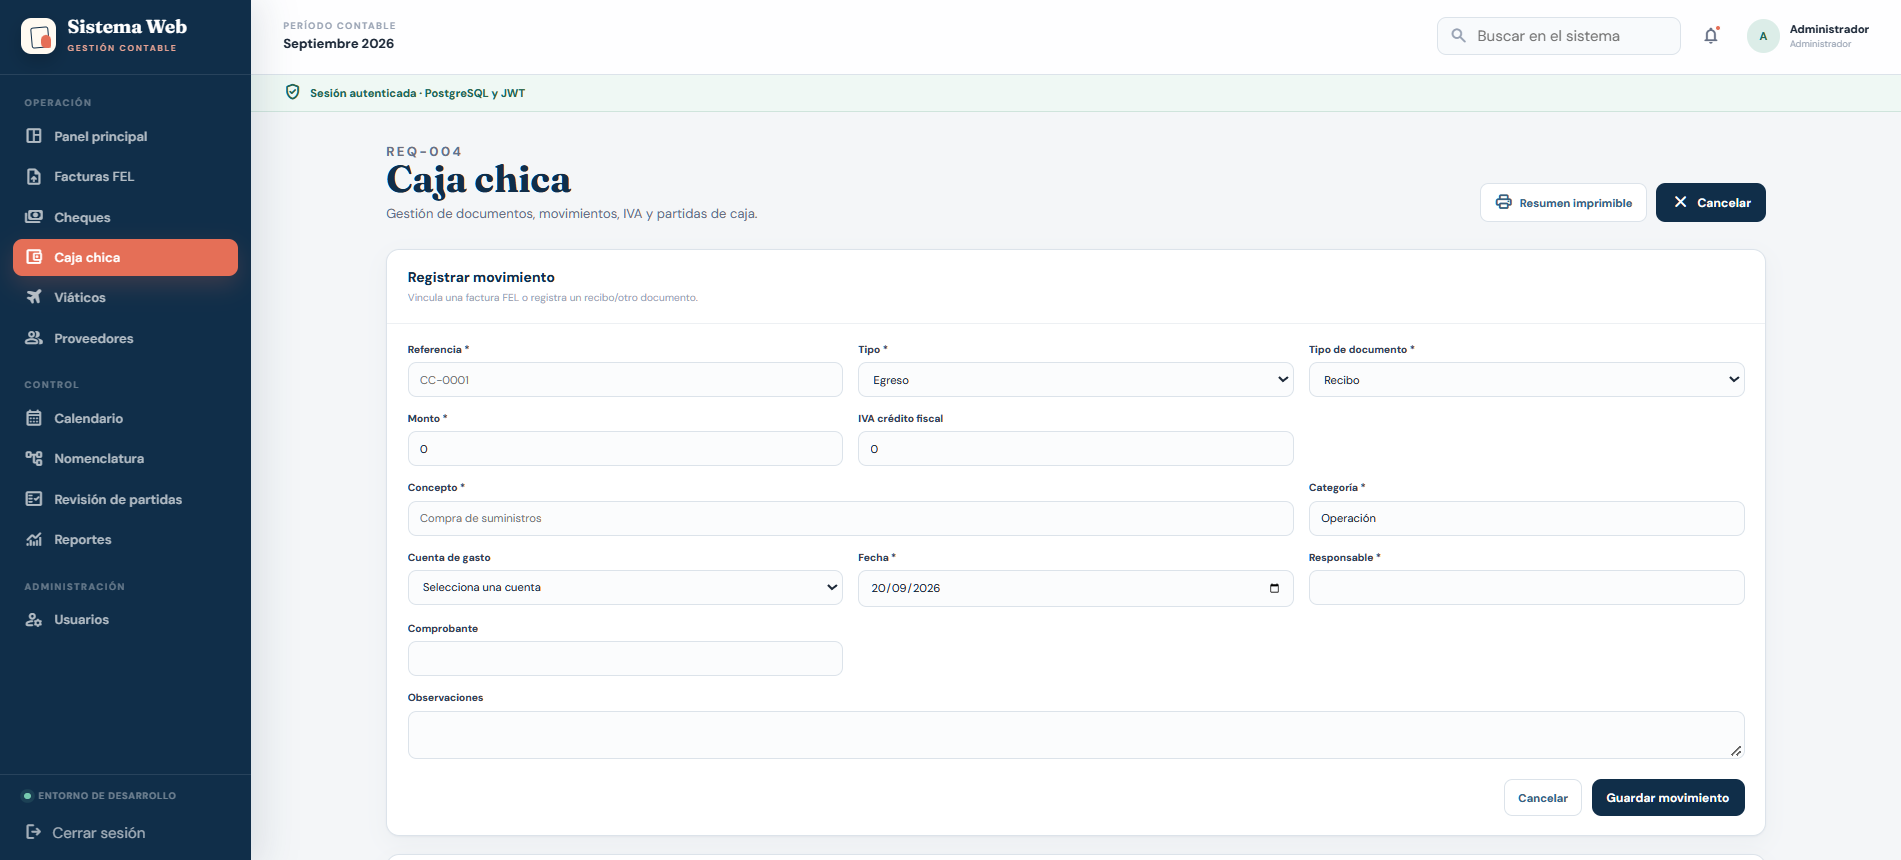
\includegraphics[width=0.96\linewidth]{capturas_reales/angular_actualizadas/formulario_caja_chica.png}
\end{figure}

% =========================================================================
% MÓDULO 4: VIÁTICOS
% =========================================================================
\subsubsection{Módulo: Viáticos}

{
\small
\setstretch{1.15}
\setlength{\parindent}{0pt}
\begin{xltabular}{\linewidth}{
    >{\raggedright\arraybackslash}p{1.3cm} 
    >{\raggedright\arraybackslash}p{2.2cm} 
    >{\raggedright\arraybackslash}>{\hsize=1.15\hsize}X 
    >{\raggedright\arraybackslash}>{\hsize=0.85\hsize}X 
    >{\centering\arraybackslash}p{0.6cm} 
    >{\raggedright\arraybackslash}p{2.0cm}
}

    % --- Encabezado de la primera página ---
    \caption{Resumen de formularios - Módulo: Viáticos} \label{tab:cap4_viaticos_resumen} \\
    \toprule
    \textbf{Código} & \textbf{Formulario} & \textbf{Propósito} & \textbf{Roles/Permisos} & \textbf{Op.} & \textbf{Ruta} \\
    \midrule
    \endfirsthead

    % --- Encabezado en páginas siguientes ---
    \toprule
    \textbf{Código} & \textbf{Formulario} & \textbf{Propósito} & \textbf{Roles/Permisos} & \textbf{Op.} & \textbf{Ruta} \\
    \midrule
    \endhead

    % --- Cierre en página intermedia ---
    \bottomrule
    \endfoot

    % --- Cierre final ---
    \bottomrule
    \endlastfoot

    % --- Filas de datos ---
    F-VIAT-01 & Gestión de Giras & Asignar territorio, colaborador y semana operativa & Admin, Encargado ({giras\_crear}) & C/U & {/viaticos} \\
    \addlinespace
    F-VIAT-02 & Asignación Factura & Vincular facturas FEL/recibos a categoría de viático & Admin, Encargado ({viaticos\_asigna}) & C & {/viaticos/asignacion} \\
    \addlinespace
    F-VIAT-03 & Generación Partida & Construir partida semanal o transitoria balanceada & Admin, Contador ({viaticos\_partida}) & C & {/viaticos} \\

\end{xltabular}
}

\paragraph{Formulario F-VIAT-02: Asignación de Facturas de Viáticos}
\noindent\textbf{Objetivo:} Asociar un comprobante de gasto a un colaborador, territorio, gira y categoría de viático (Viáticos, Movilidad o Actividades). \\[0.3em]
\textbf{Ubicación / Ruta:} Viáticos $\rightarrow$ Asignación de facturas ({/viaticos/asignacion}). \\[0.3em]
\textbf{Roles/Permisos:} Admin, Encargado ({viaticos\_asigna}). \\[0.3em]
\textbf{Campos clave y validaciones críticas:} {colaborador} (Seleccionado del catálogo de colaboradores activos); {territorio\_gira} (Requerido, debe coincidir con la semana programada); {categoria\_gasto} (Requerida: Viáticos, Movilidad, Actividades. Regla: Movilidad solo permitida la 1era semana del mes); {numero\_factura} (Requerido, no reutilizable en otra gira); {cuenta\_contable} (Requerida, seleccionada del catálogo de Nomenclatura). \\[0.3em]
\textbf{Flujo:} Seleccionar colaborador y gira $\rightarrow$ Ingresar número de factura $\rightarrow$ Asignar categoría y cuenta contable $\rightarrow$ Guardar asignación. \\[0.3em]
\textbf{Mensaje principal del sistema:} ``Factura asignada a gira correctamente.''

\begin{figure}[H]
    \centering
    \caption{Formulario de asignación de facturas a giras y viáticos.}
    \label{fig:cap4_viaticos_pantalla}
    \vspace{0.2cm}
    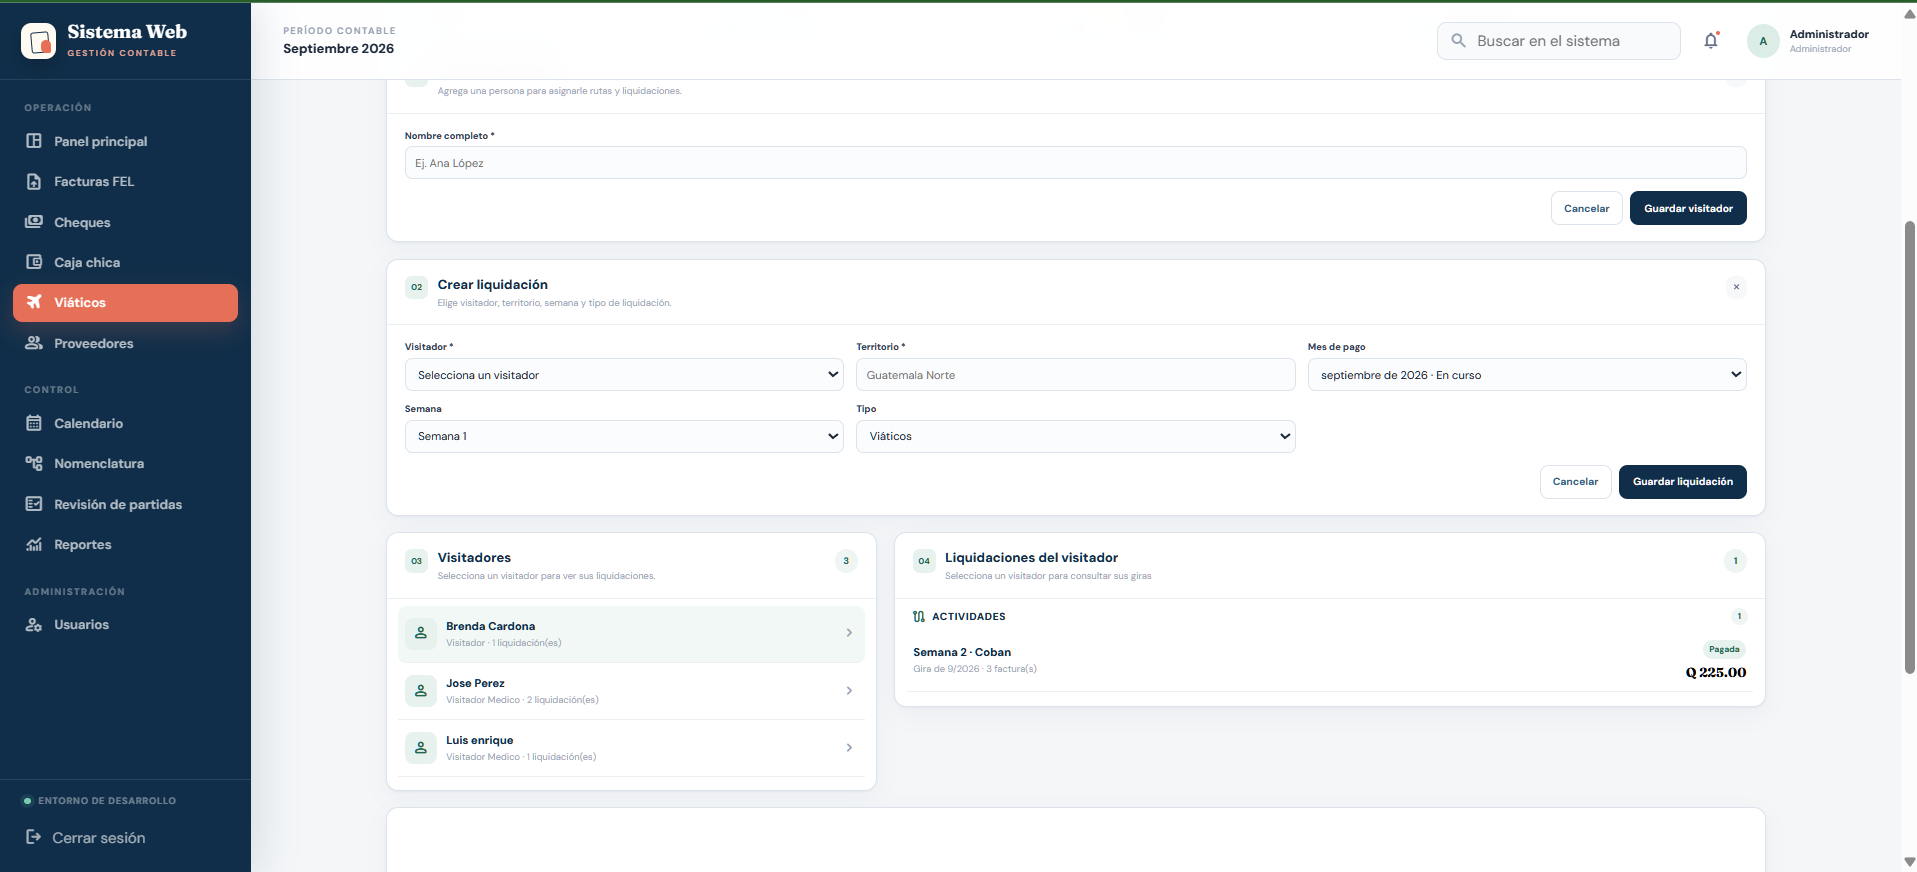
\includegraphics[width=0.96\linewidth]{capturas_reales/angular_actualizadas/pantalla_07_viaticos_nueva_liquidacion.png}
\end{figure}

% =========================================================================
% MÓDULO 5: PROVEEDORES
% =========================================================================
\subsubsection{Módulo: Proveedores}

{
\small
\setstretch{1.15}
\setlength{\parindent}{0pt}
\begin{xltabular}{\linewidth}{
    >{\raggedright\arraybackslash}p{1.3cm} 
    >{\raggedright\arraybackslash}p{2.2cm} 
    >{\raggedright\arraybackslash}>{\hsize=1.15\hsize}X 
    >{\raggedright\arraybackslash}>{\hsize=0.85\hsize}X 
    >{\centering\arraybackslash}p{0.6cm} 
    >{\raggedright\arraybackslash}p{2.0cm}
}

    % --- Encabezado de la primera página ---
    \caption{Resumen de formularios - Módulo: Proveedores} \label{tab:cap4_proveedores_resumen} \\
    \toprule
    \textbf{Código} & \textbf{Formulario} & \textbf{Propósito} & \textbf{Roles/Permisos} & \textbf{Op.} & \textbf{Ruta} \\
    \midrule
    \endfirsthead

    % --- Encabezado en páginas siguientes ---
    \toprule
    \textbf{Código} & \textbf{Formulario} & \textbf{Propósito} & \textbf{Roles/Permisos} & \textbf{Op.} & \textbf{Ruta} \\
    \midrule
    \endhead

    % --- Cierre en página intermedia ---
    \bottomrule
    \endfoot

    % --- Cierre final ---
    \bottomrule
    \endlastfoot

    % --- Filas de datos ---
    F-PROV-01 & Registro Proveedor & Alta por NIT, datos comerciales y condiciones de pago & Admin, Compras, Contador ({proveedores\_crear}) & C/U & {/proveedores} \\
    \addlinespace
    F-PROV-02 & Cartera y Facturas & Consultar saldos, crédito, retenciones e historial & Admin, Contador ({proveedores\_ver}) & R & {/proveedores} \\
    \addlinespace
    F-PROV-03 & Generación Partida & Crear partida dentro del mes o transitoria & Admin, Contador ({proveedores\_partida}) & C & {/proveedores} \\

\end{xltabular}
}

\paragraph{Formulario F-PROV-01: Registro y Configuración de Proveedores}
\noindent\textbf{Objetivo:} Crear y mantener el registro maestro de proveedores con su NIT, nombre comercial, retenciones autorizadas y cuenta contable por defecto. \\[0.3em]
\textbf{Ubicación / Ruta:} Módulo Proveedores $\rightarrow$ Nuevo proveedor ({/proveedores}). \\[0.3em]
\textbf{Roles/Permisos:} Admin, Compras, Contador ({proveedores\_crear}). \\[0.3em]
\textbf{Campos clave y validaciones críticas:} {nit\_proveedor} (Requerido, único, formato tributario guatemalteco); {nombre\_comercial} y {razon\_social} (Requeridos); {dias\_credito} (Integer $\ge 0$, ej.: 30 días); {aplica\_retencion\_isr} / {iva} (Boolean); {cuenta\_nomenclatura\_id} (Requerido, enlace a Nomenclatura Contable). \\[0.3em]
\textbf{Flujo:} Hacer clic en ``Nuevo proveedor'' $\rightarrow$ Ingresar NIT para autocompletado/verificación $\rightarrow$ Asignar cuenta contable y condiciones de crédito $\rightarrow$ Guardar registro. \\[0.3em]
\textbf{Mensaje principal del sistema:} ``Proveedor registrado exitosamente.''

\begin{figure}[H]
    \centering
    \caption{Módulo de Proveedores con cartera de crédito y gestión de partidas.}
    \label{fig:cap4_proveedores_pantalla}
    \vspace{0.2cm}
    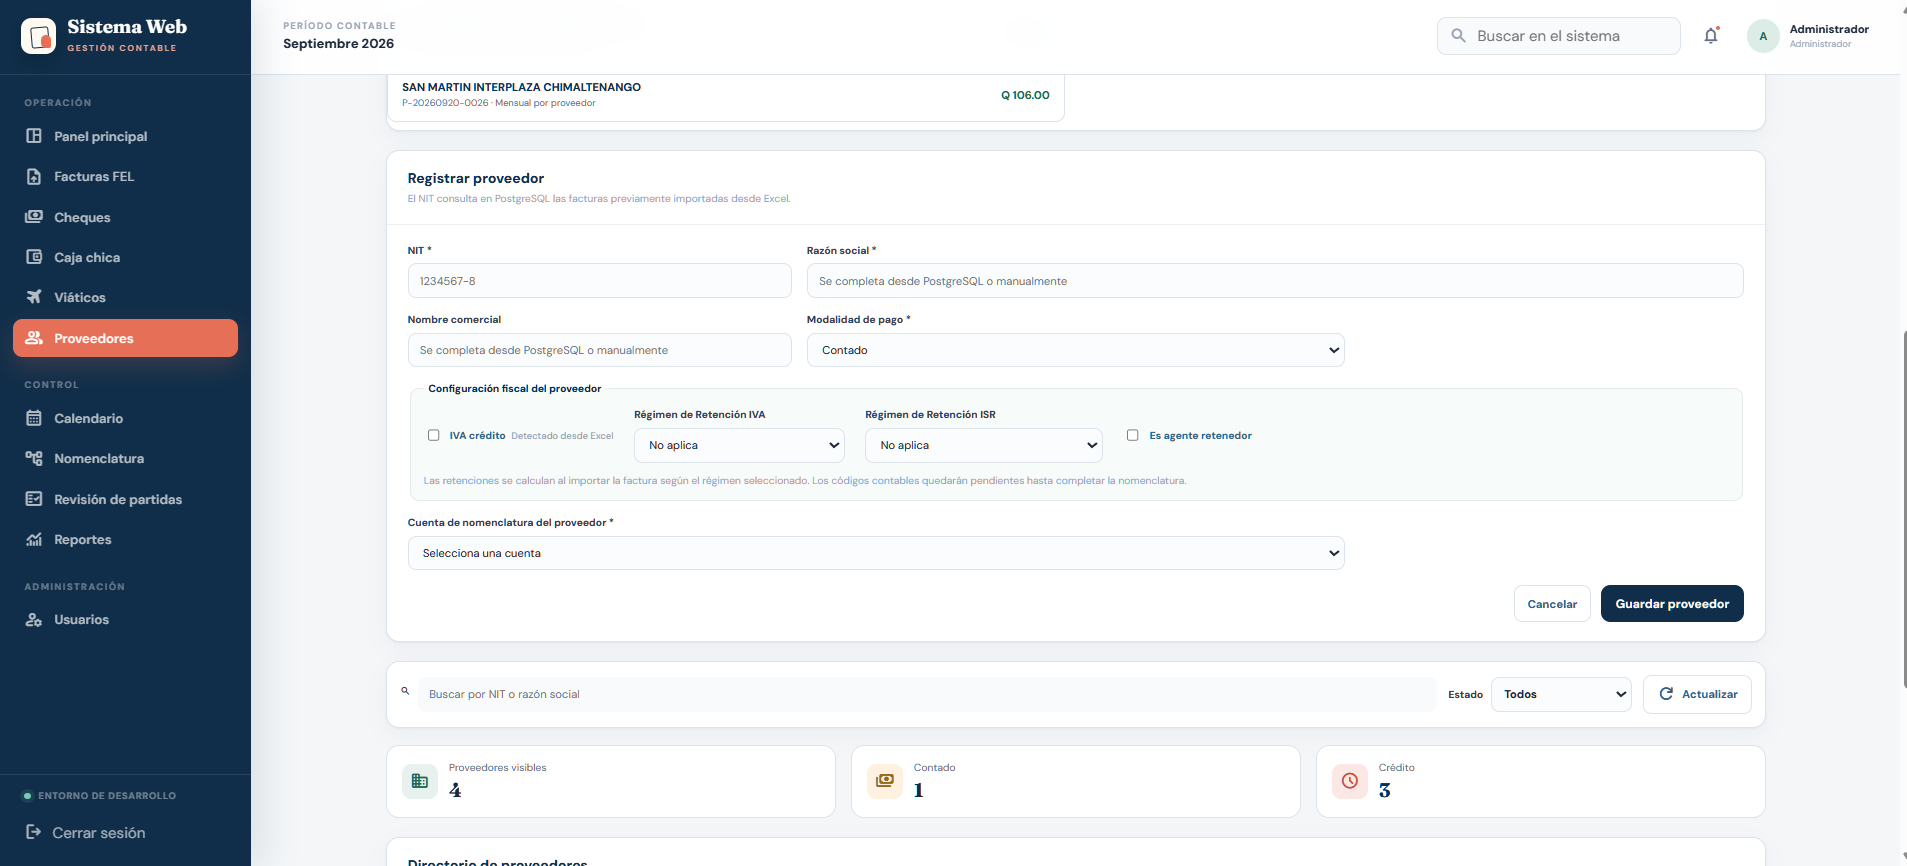
\includegraphics[width=0.96\linewidth]{capturas_reales/angular_actualizadas/pantalla_08_proveedores_nuevo.png}
\end{figure}

% =========================================================================
% MÓDULO 6: CALENDARIO OPERATIVO
% =========================================================================
\subsubsection{Módulo: Calendario Operativo}

{
\small
\setstretch{1.15}
\setlength{\parindent}{0pt}
\begin{xltabular}{\linewidth}{
    >{\raggedright\arraybackslash}p{1.3cm} 
    >{\raggedright\arraybackslash}p{2.2cm} 
    >{\raggedright\arraybackslash}>{\hsize=1.15\hsize}X 
    >{\raggedright\arraybackslash}>{\hsize=0.85\hsize}X 
    >{\centering\arraybackslash}p{0.6cm} 
    >{\raggedright\arraybackslash}p{2.0cm}
}

    % --- Encabezado de la primera página ---
    \caption{Resumen de formularios - Módulo: Calendario Operativo} \label{tab:cap4_calendario_resumen} \\
    \toprule
    \textbf{Código} & \textbf{Formulario} & \textbf{Propósito} & \textbf{Roles/Permisos} & \textbf{Op.} & \textbf{Ruta} \\
    \midrule
    \endfirsthead

    % --- Encabezado en páginas siguientes ---
    \toprule
    \textbf{Código} & \textbf{Formulario} & \textbf{Propósito} & \textbf{Roles/Permisos} & \textbf{Op.} & \textbf{Ruta} \\
    \midrule
    \endhead

    % --- Cierre en página intermedia ---
    \bottomrule
    \endfoot

    % --- Cierre final ---
    \bottomrule
    \endlastfoot

    % --- Filas de datos ---
    F-CAL-01 & Vista Calendario & Consultar eventos, pagos, depósitos y giras & Todos ({calendario\_ver}) & R & {/calendario} \\
    \addlinespace
    F-CAL-02 & Evento / Actividad & Programar nueva actividad contable u operativa & Admin, Encargado ({calendario\_crear}) & C/U & {/calendario} \\

\end{xltabular}
}

\paragraph{Formulario F-CAL-02: Programación de Actividades y Eventos}
\noindent\textbf{Objetivo:} Programar eventos financieros como fechas de depósito de cheques posfechados, vencimiento de facturas de proveedores o inicio de giras. \\[0.3em]
\textbf{Ubicación / Ruta:} Módulo Calendario $\rightarrow$ Nueva Actividad ({/calendario}). \\[0.3em]
\textbf{Roles/Permisos:} Admin, Encargado ({calendario\_crear}). \\[0.3em]
\textbf{Campos clave y validaciones críticas:} {titulo\_evento} (Requerido, ej.: ``Pago Proveedor Distribuidora X''); {fecha\_inicio} y {fecha\_fin} (Requeridas, {fecha\_fin} $\ge$ {fecha\_inicio}); {tipo\_actividad} (Requerido: Pago, Cheque, Gira, Auditoría); {prioridad} (Alta, Media, Baja). \\[0.3em]
\textbf{Flujo:} Seleccionar fecha en el calendario o presionar ``Actividad'' $\rightarrow$ Llenar detalles del evento $\rightarrow$ Guardar $\rightarrow$ Actualización dinámica en el calendario. \\[0.3em]
\textbf{Mensaje principal del sistema:} ``Evento agregado al calendario operativo.''

\begin{figure}[H]
    \centering
    \caption{Módulo de Calendario Operativo con eventos y vencimientos anotados.}
    \label{fig:cap4_calendario_pantalla}
    \vspace{0.2cm}
    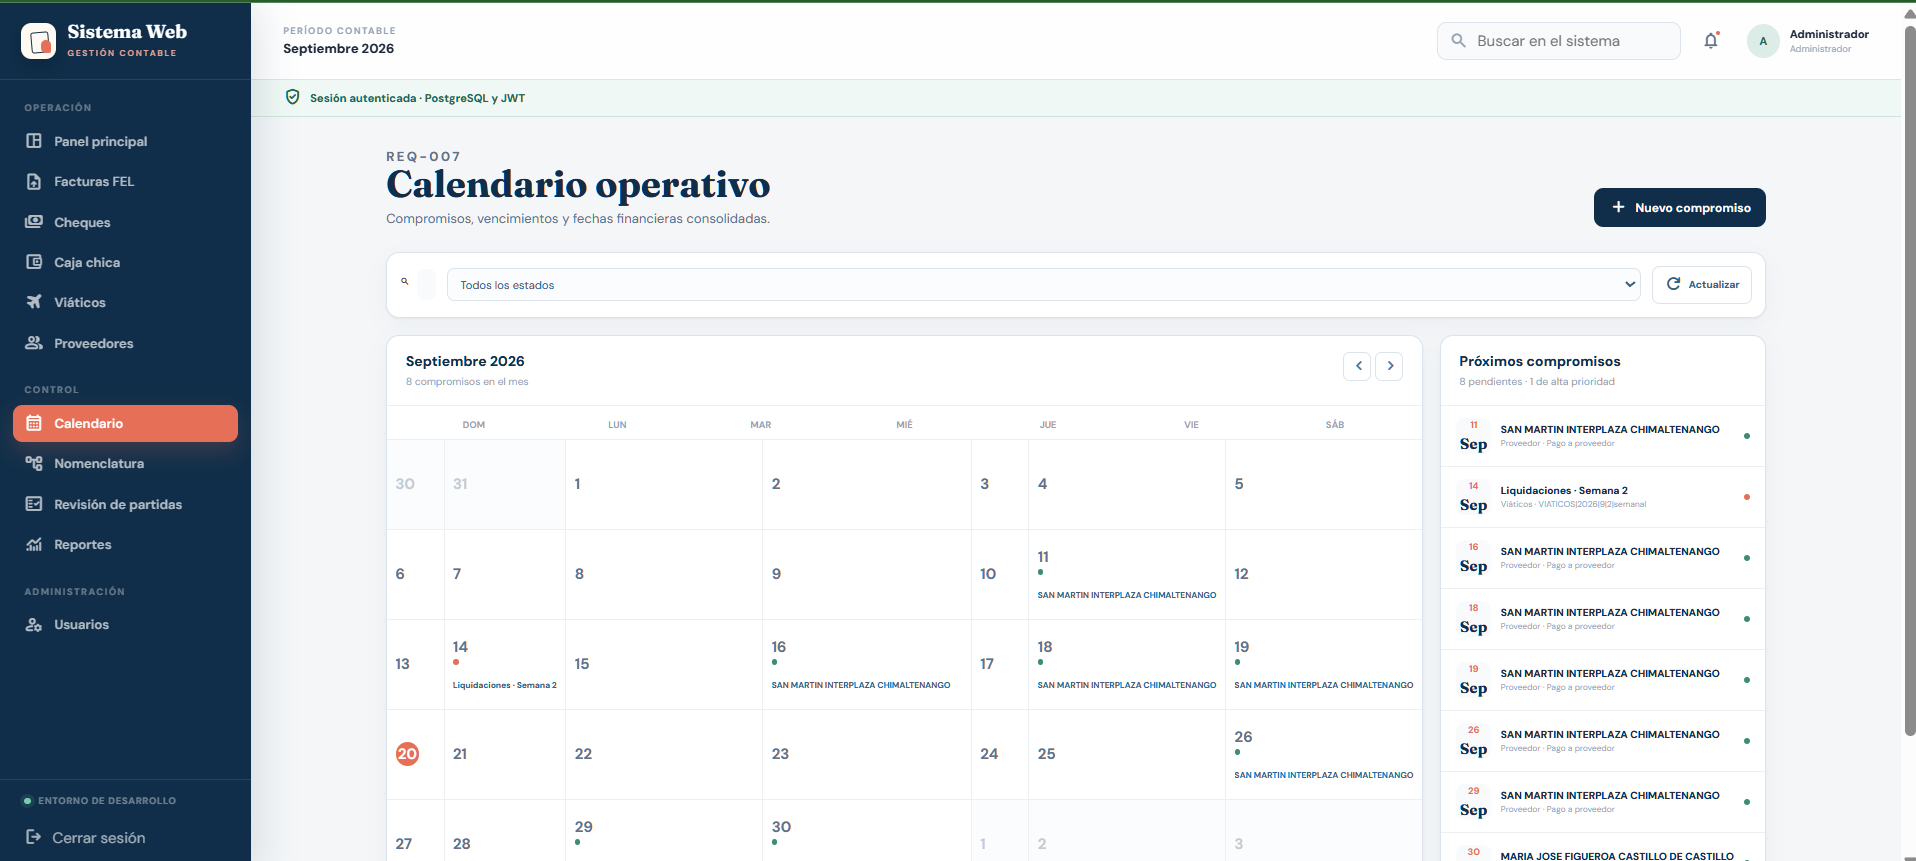
\includegraphics[width=0.96\linewidth]{capturas_reales/angular_actualizadas/pantalla_09_calendario.png}
\end{figure}

% =========================================================================
% MÓDULO 7: NOMENCLATURA CONTABLE
% =========================================================================
\subsubsection{Módulo: Nomenclatura Contable}

{
\small
\setstretch{1.15}
\setlength{\parindent}{0pt}
\begin{xltabular}{\linewidth}{
    >{\raggedright\arraybackslash}p{1.3cm} 
    >{\raggedright\arraybackslash}p{2.2cm} 
    >{\raggedright\arraybackslash}>{\hsize=1.15\hsize}X 
    >{\raggedright\arraybackslash}>{\hsize=0.85\hsize}X 
    >{\centering\arraybackslash}p{0.6cm} 
    >{\raggedright\arraybackslash}p{2.0cm}
}

    % --- Encabezado de la primera página ---
    \caption{Resumen de formularios - Módulo: Nomenclatura Contable} \label{tab:cap4_nomenclatura_resumen} \\
    \toprule
    \textbf{Código} & \textbf{Formulario} & \textbf{Propósito} & \textbf{Roles/Permisos} & \textbf{Op.} & \textbf{Ruta} \\
    \midrule
    \endfirsthead

    % --- Encabezado en páginas siguientes ---
    \toprule
    \textbf{Código} & \textbf{Formulario} & \textbf{Propósito} & \textbf{Roles/Permisos} & \textbf{Op.} & \textbf{Ruta} \\
    \midrule
    \endhead

    % --- Cierre en página intermedia ---
    \bottomrule
    \endfoot

    % --- Cierre final ---
    \bottomrule
    \endlastfoot

    % --- Filas de datos ---
    F-NOM-01 & Catálogo Cuentas & Listar, buscar y filtrar catálogo de cuentas & Admin, Contador ({nomenclatura\_ver}) & R & {/nomenclatura} \\
    \addlinespace
    F-NOM-02 & Formulario Cuenta & Crear o editar código, nombre y naturaleza de cuenta & Admin, Contador ({nomenclatura\_crear}) & C/U & {/nomenclatura} \\

\end{xltabular}
}

\paragraph{Formulario F-NOM-02: Formulario de Cuenta Contable}
\noindent\textbf{Objetivo:} Crear y actualizar la estructura del plan de cuentas (Nomenclatura) indicando el código jerárquico y la naturaleza contable (Debe / Haber). \\[0.3em]
\textbf{Ubicación / Ruta:} Nomenclatura $\rightarrow$ Nueva Cuenta / Editar ({/nomenclatura}). \\[0.3em]
\textbf{Roles/Permisos:} Admin, Contador ({nomenclatura\_crear}). \\[0.3em]
\textbf{Campos clave y validaciones críticas:} {codigo\_cuenta} (Requerido, único, formato estructurado, ej.: {5.1.01.001}); {nombre\_cuenta} (Requerido, ej.: ``Gastos de Operación'').

\subsubsection{Módulo: Autenticación y Gestión de Usuarios}
La Tabla~\ref{tab:cap4_auth_resumen} resume el formulario de acceso y la administración de credenciales y roles.

{
\small
\setstretch{1.15}
\setlength{\parindent}{0pt}
\begin{xltabular}{\linewidth}{
    >{\raggedright\arraybackslash}p{1.3cm} 
    >{\raggedright\arraybackslash}p{2.2cm} 
    >{\raggedright\arraybackslash}>{\hsize=1.15\hsize}X 
    >{\raggedright\arraybackslash}>{\hsize=0.85\hsize}X 
    >{\centering\arraybackslash}p{0.6cm} 
    >{\raggedright\arraybackslash}p{2.0cm}
}
\caption{Resumen de formularios - Módulo: Autenticación y gestión de usuarios}\label{tab:cap4_auth_resumen}\\
\toprule
\textbf{Código} & \textbf{Formulario} & \textbf{Propósito} & \textbf{Roles/Permisos} & \textbf{Op.} & \textbf{Ruta}\\
\midrule
\endfirsthead
\toprule
\textbf{Código} & \textbf{Formulario} & \textbf{Propósito} & \textbf{Roles/Permisos} & \textbf{Op.} & \textbf{Ruta}\\
\midrule
\endhead
\bottomrule
\endfoot
\bottomrule
\endlastfoot
F-AUTH-01 & Inicio de sesión & Validar credenciales y habilitar la sesión autorizada & Usuario registrado ({iniciar\_sesion}) & C/R & {/login}\\
\addlinespace
F-AUTH-02 & Usuarios y roles & Registrar usuarios y asignar permisos de acceso & Admin ({gestionar\_usuarios}) & CRUD & {/usuarios}\\
\end{xltabular}
}

\paragraph{Formulario F-AUTH-01: Inicio de sesión}
\noindent\textbf{Objetivo:} Validar el usuario y la contraseña antes de permitir el acceso al Panel principal. \textbf{Campos y validaciones:} usuario requerido, contraseña requerida y mensaje controlado para credenciales inválidas. \textbf{Flujo:} ingresar credenciales $\rightarrow$ presionar ``Ingresar al sistema'' $\rightarrow$ validar sesión $\rightarrow$ mostrar el Panel principal.

\begin{figure}[H]
    \centering
    \caption{Pantalla de inicio de sesión del sistema.}
    \label{fig:cap4_auth_pantalla}
    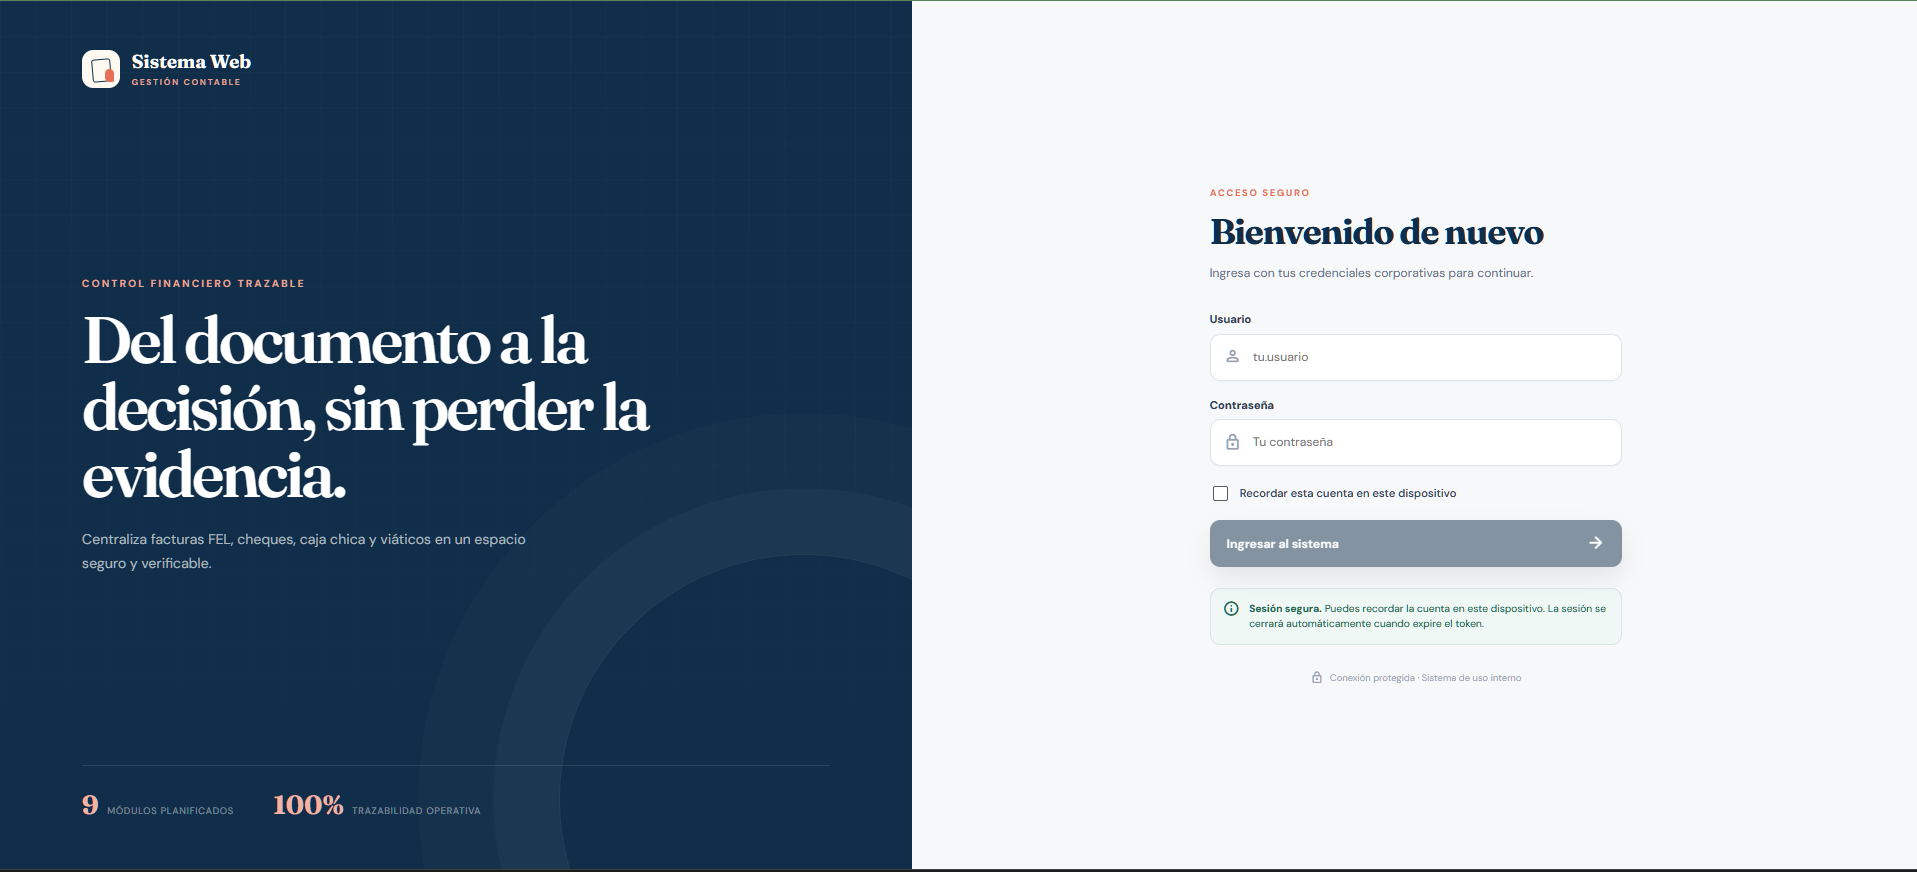
\includegraphics[width=0.96\linewidth]{capturas_reales/angular_actualizadas/pantalla_01_login.png}
\end{figure}

\subsubsection{Módulo: Reportes Operativos y Financieros}
La Tabla~\ref{tab:cap4_reportes_resumen} documenta las funciones de consulta y generación de reportes autorizados.

{
\small
\setstretch{1.15}
\setlength{\parindent}{0pt}
\begin{xltabular}{\linewidth}{
    >{\raggedright\arraybackslash}p{1.3cm} 
    >{\raggedright\arraybackslash}p{2.2cm} 
    >{\raggedright\arraybackslash}>{\hsize=1.15\hsize}X 
    >{\raggedright\arraybackslash}>{\hsize=0.85\hsize}X 
    >{\centering\arraybackslash}p{0.6cm} 
    >{\raggedright\arraybackslash}p{2.0cm}
}
\caption{Resumen de formularios - Módulo: Reportes operativos y financieros}\label{tab:cap4_reportes_resumen}\\
\toprule
\textbf{Código} & \textbf{Formulario} & \textbf{Propósito} & \textbf{Roles/Permisos} & \textbf{Op.} & \textbf{Ruta}\\
\midrule
\endfirsthead
\toprule
\textbf{Código} & \textbf{Formulario} & \textbf{Propósito} & \textbf{Roles/Permisos} & \textbf{Op.} & \textbf{Ruta}\\
\midrule
\endhead
\bottomrule
\endfoot
\bottomrule
\endlastfoot
F-REP-01 & Consulta de reportes & Filtrar información por período, módulo y estado & Admin, Contador ({consultar\_reportes}) & R & {/reportes}\\
\addlinespace
F-REP-02 & Resumen de Caja chica & Revisar e imprimir los movimientos del fondo & Admin, Contador ({consultar\_caja}) & R & {/reportes/caja-chica}\\
\end{xltabular}
}

\paragraph{Formulario F-REP-01: Consulta de reportes}
\noindent\textbf{Objetivo:} Presentar información consolidada para revisión operativa y financiera. \textbf{Campos y validaciones:} período requerido, módulo opcional y estado válido. \textbf{Flujo:} seleccionar filtros $\rightarrow$ consultar $\rightarrow$ revisar resultados $\rightarrow$ imprimir o guardar el reporte autorizado.

\begin{figure}[H]
    \centering
    \caption{Pantalla de reportes operativos y financieros.}
    \label{fig:cap4_reportes_pantalla}
    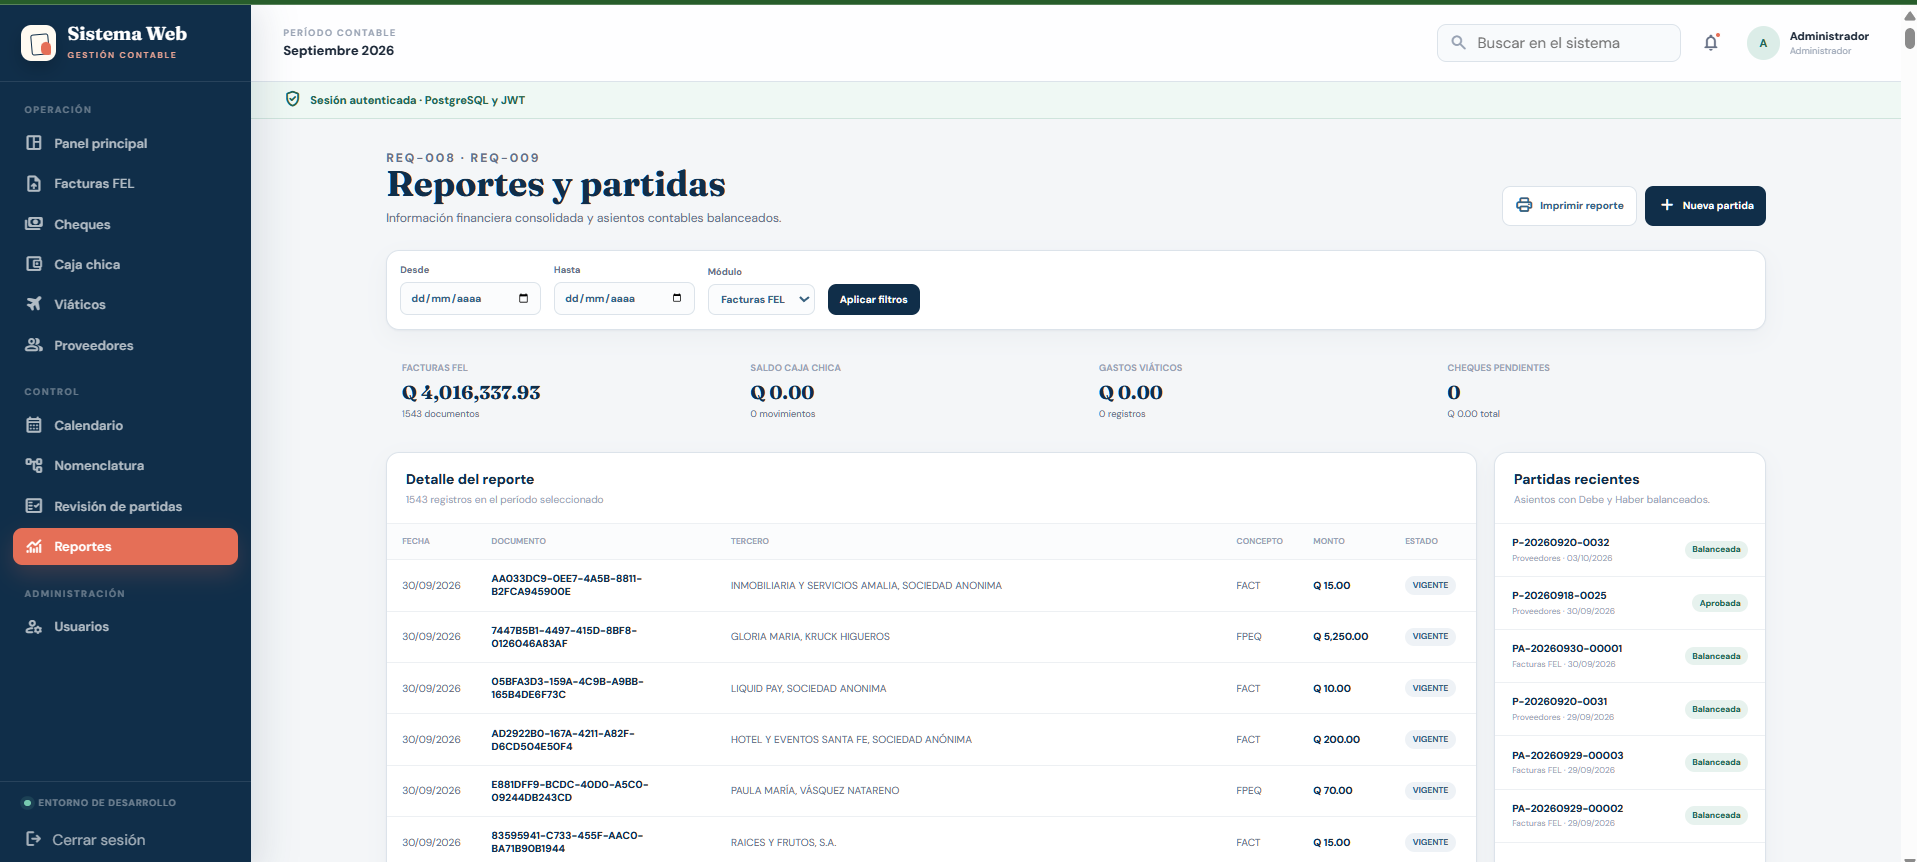
\includegraphics[width=0.96\linewidth]{capturas_reales/angular_actualizadas/pantalla_11_reportes.png}
\end{figure}

\subsection{Fragmentos de Código}
\label{sec:cap4_fragmentos_codigo}

De conformidad con los lineamientos metodológicos, en este apartado se documenta el desarrollo técnico del sistema mediante ocho fragmentos representativos y demostrativos de código fuente, preparados para ilustrar la lógica correspondiente a cada módulo. Cada extracto incluye su especificación de módulo, lenguaje utilizado, bloque de código en fuente monoespaciada, descripción funcional y la evidencia correspondiente a la interfaz de usuario real.

% =========================================================================
% FRAGMENTO 1: FACTURAS FEL (PYTHON/FASTAPI)
% =========================================================================
\subsubsection{Fragmento 1: Procesamiento y Validación de DTE FEL}
\noindent\textbf{Módulo:} Facturas FEL/SAT \\
\textbf{Lenguaje:} Python (FastAPI)

A continuación, se presenta el fragmento de código encargado de procesar la estructura XML de las facturas electrónicas y verificar la no duplicidad del UUID tributario:

\begin{minted}[breaklines, fontsize=\normalsize]{python}
@router.post("/importar-xml")
async def importar_xml_fel(file: UploadFile = File(...), db: Session = Depends(get_db)):
    if not file.filename.endswith('.xml'):
        raise HTTPException(status_code=400, detail="Formato de archivo invalido")
    
    content = await file.read()
    tree = ET.fromstring(content)
    uuid_dte = tree.find(".//{http://www.sat.gob.gt/dte/fel/0.1.0}NumeroAutorizacion").text
    
    existe = db.query(FacturaFEL).filter(FacturaFEL.uuid == uuid_dte).first()
    if existe:
        raise HTTPException(status_code=400, detail="El DTE ya se encuentra registrado")
    
    nueva_factura = FacturaFEL(uuid=uuid_dte, estado="PENDIENTE")
    db.add(nueva_factura)
    db.commit()
    return {"status": "exito", "uuid": uuid_dte}
\end{minted}

\noindent\textbf{Descripción:} Este código pertenece al backend del módulo de Facturas FEL/SAT. Su función principal es recibir la carga de archivos XML, analizar el árbol DOM para extraer el UUID oficial emitido por la SAT y validar en la base de datos que el documento no haya sido ingresado previamente.

\begin{figure}[H]
    \centering
    \caption{Formulario de carga masiva e importación de comprobantes FEL.}
    \label{fig:cap4_code_fel_xml}
    \vspace{0.2cm}
    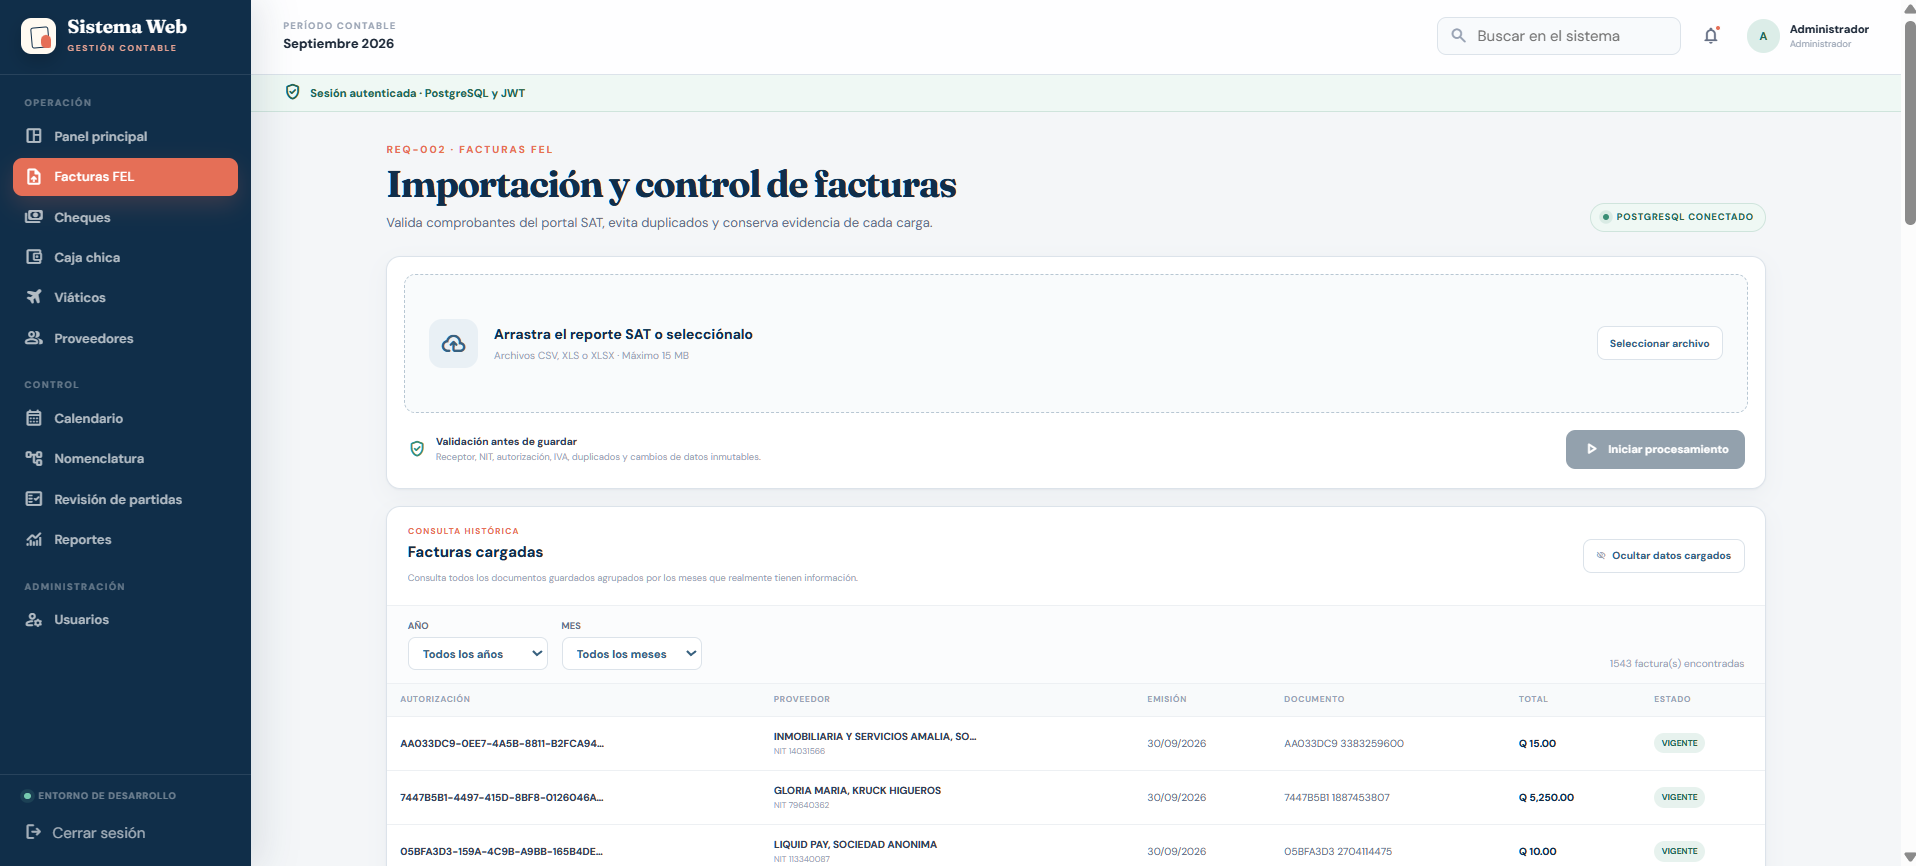
\includegraphics[width=0.96\linewidth]{capturas_reales/angular_actualizadas/pantalla_03_facturas_fel.png}
    \vspace{0.1cm}
    \begin{minipage}{0.96\linewidth}
        \small\textit{Nota.} La captura de pantalla corresponde al formulario web real que consume el endpoint de validación de archivos XML.
    \end{minipage}
\end{figure}

% =========================================================================
% FRAGMENTO 2: CHEQUES POSFECHADOS (PYTHON/FASTAPI)
% =========================================================================
\subsubsection{Fragmento 2: Registro y Validación de Cheques Posfechados}
\noindent\textbf{Módulo:} Cheques Posfechados \\
\textbf{Lenguaje:} Python (FastAPI)

A continuación, se presenta la lógica de validación de fechas y montos en el registro de cheques posfechados:

\begin{minted}[breaklines, fontsize=\small]{python}
@router.post("/cheques")
def crear_cheque(cheque: ChequeCreate, db: Session = Depends(get_db)):
    if cheque.fecha_deposito < cheque.fecha_recepcion:
        raise HTTPException(status_code=400, detail="La fecha de deposito debe ser mayor o igual a la de recepcion")
    
    if cheque.monto <= 0:
        raise HTTPException(status_code=400, detail="El monto del cheque debe ser mayor a cero")
        
    nuevo_cheque = Cheque(**cheque.dict(), estado="PENDIENTE")
    db.add(nuevo_cheque)
    db.commit()
    db.refresh(nuevo_cheque)
    return nuevo_cheque
\end{minted}

\noindent\textbf{Descripción:} El fragmento corresponde a la capa de servicios del módulo de Cheques Posfechados. Garantiza la coherencia cronológica de las fechas de depósito respecto a las de recepción y asegura que únicamente se registren montos financieros válidos antes de persistir la información.

\begin{figure}[H]
    \centering
    \caption{Formulario de gestión e ingreso de cheques posfechados.}
    \label{fig:cap4_code_cheques}
    \vspace{0.2cm}
    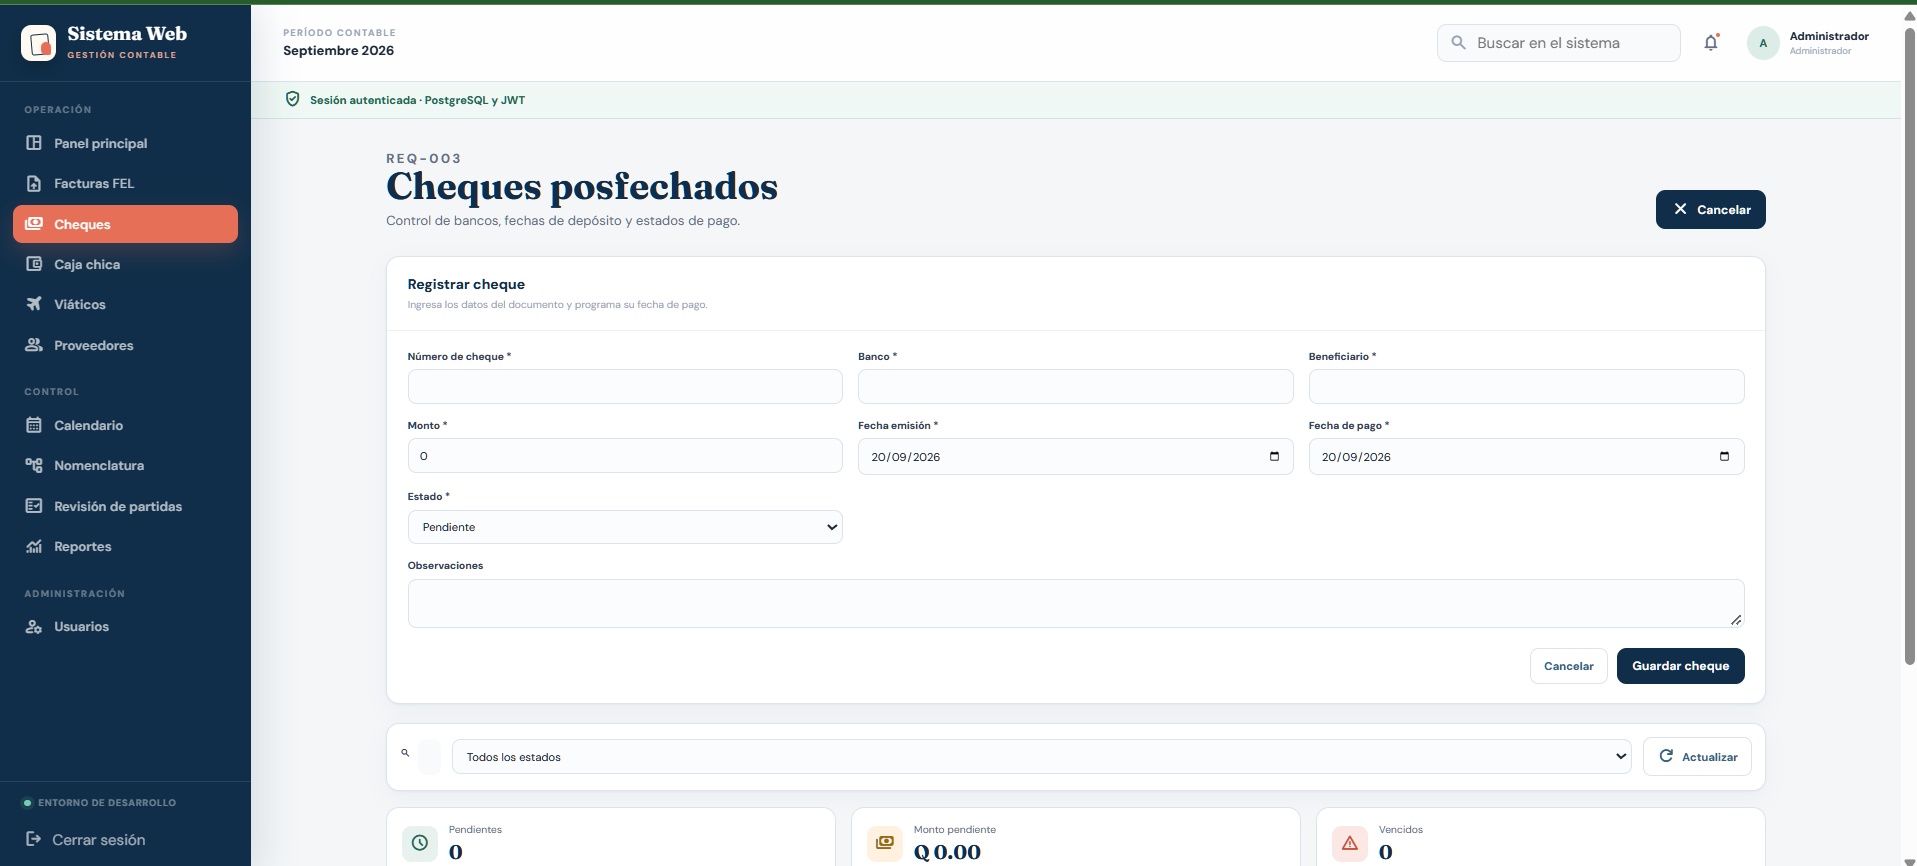
\includegraphics[width=0.96\linewidth]{capturas_reales/angular_actualizadas/formulario_cheque.png}
    \vspace{0.1cm}
    \begin{minipage}{0.96\linewidth}
        \small\textit{Nota.} La captura de pantalla ilustra la interfaz de registro de cheques respaldada por el método de verificación en backend.
    \end{minipage}
\end{figure}

% =========================================================================
% FRAGMENTO 3: CAJA CHICA (PYTHON/FASTAPI)
% =========================================================================
\subsubsection{Fragmento 3: Control de Disponible y Registro de Egresos}
\noindent\textbf{Módulo:} Caja Chica \\
\textbf{Lenguaje:} Python (FastAPI)

A continuación, se expone la función encargada de verificar la disponibilidad de saldo en el fondo fijo previo al registro de un recibo de egreso:

\begin{minted}[breaklines, fontsize=\small]{python}
@router.post("/caja-chica/recibo")
def registrar_recibo(recibo: ReciboCreate, db: Session = Depends(get_db)):
    fondo = db.query(FondoCajaChica).filter(FondoCajaChica.activo == True).first()
    if not fondo:
        raise HTTPException(status_code=404, detail="No existe un fondo de caja chica activo")
        
    if recibo.monto_total > fondo.saldo_disponible:
        raise HTTPException(status_code=400, detail="El monto excede el saldo disponible del fondo")
        
    fondo.saldo_disponible -= recibo.monto_total
    nuevo_movimiento = MovimientoCaja(**recibo.dict(), fondo_id=fondo.id)
    db.add(nuevo_movimiento)
    db.commit()
    return nuevo_movimiento
\end{minted}

\noindent\textbf{Descripción:} Este código corresponde a la lógica de negocio de Caja Chica. Evalúa que la caja posea saldo suficiente para cubrir el gasto solicitado y efectúa el débito automático sobre el fondo asignado al momento de guardar el recibo.

\begin{figure}[H]
    \centering
    \caption{Formulario para captura de recibos y egresos de Caja Chica.}
    \label{fig:cap4_code_caja}
    \vspace{0.2cm}
    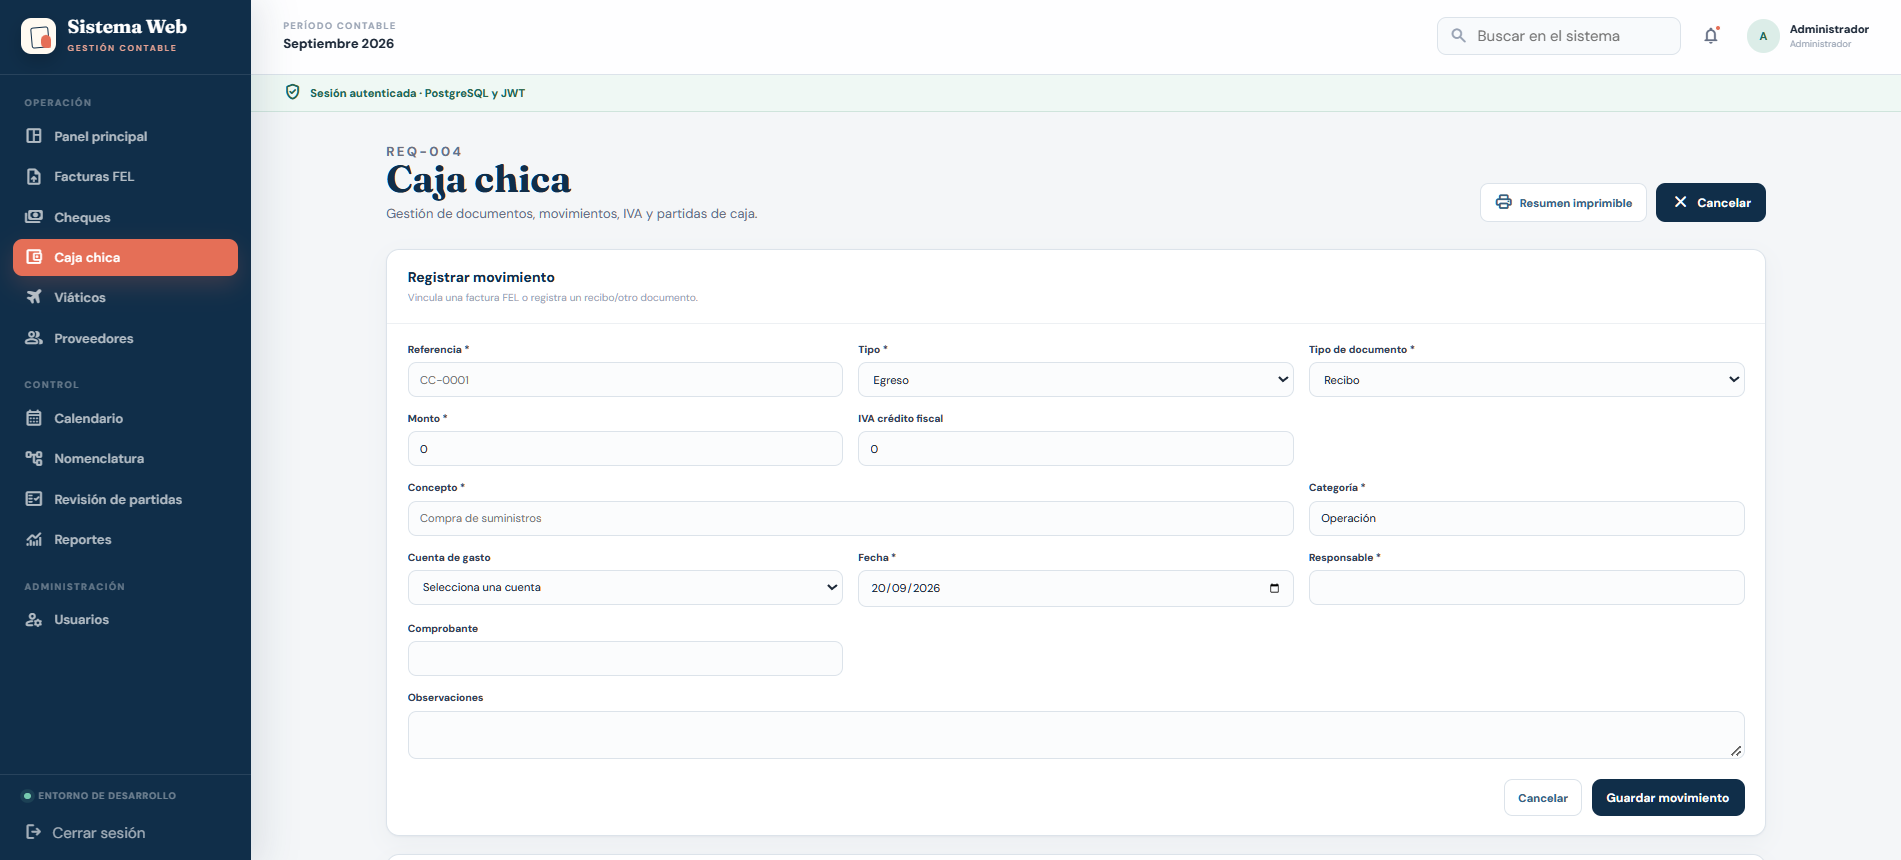
\includegraphics[width=0.96\linewidth]{capturas_reales/angular_actualizadas/formulario_caja_chica.png}
    \vspace{0.1cm}
    \begin{minipage}{0.96\linewidth}
        \small\textit{Nota.} La captura muestra la pantalla interactiva de la caja chica donde el usuario liquida recibos bajo la regla de saldo disponible.
    \end{minipage}
\end{figure}

% =========================================================================
% FRAGMENTO 4: VIÁTICOS (TYPESCRIPT/ANGULAR)
% =========================================================================
\subsubsection{Fragmento 4: Regla de Asignación por Categoría de Viático}
\noindent\textbf{Módulo:} Viáticos \\
\textbf{Lenguaje:} TypeScript (Angular)

A continuación, se muestra el método de validación en frontend para restringir categorías de gastos según el calendario operativo de la gira:

\begin{minted}[breaklines, fontsize=\small]{python}
validarCategoriaGasto(semanaGira: number, categoriaSeleccionada: string): boolean {
  if (categoriaSeleccionada === 'MOVILIDAD' && semanaGira !== 1) {
    this.toastr.warning('La categoria Movilidad solo esta permitida durante la primera semana');
    this.formularioAsignacion.get('categoria_gasto')?.setValue('');
    return false;
  }
  return true;
}
\end{minted}

\noindent\textbf{Descripción:} El fragmento forma parte de la lógica del componente frontend en el módulo de Viáticos. Ejecuta una validación reactiva que prohíbe la selección de rubros de movilidad fuera de la primera semana operativa del mes, alertando al usuario mediante notificaciones.

\begin{figure}[H]
    \centering
    \caption{Formulario de asignación de facturas a giras y categorías de viáticos.}
    \label{fig:cap4_code_viaticos}
    \vspace{0.2cm}
    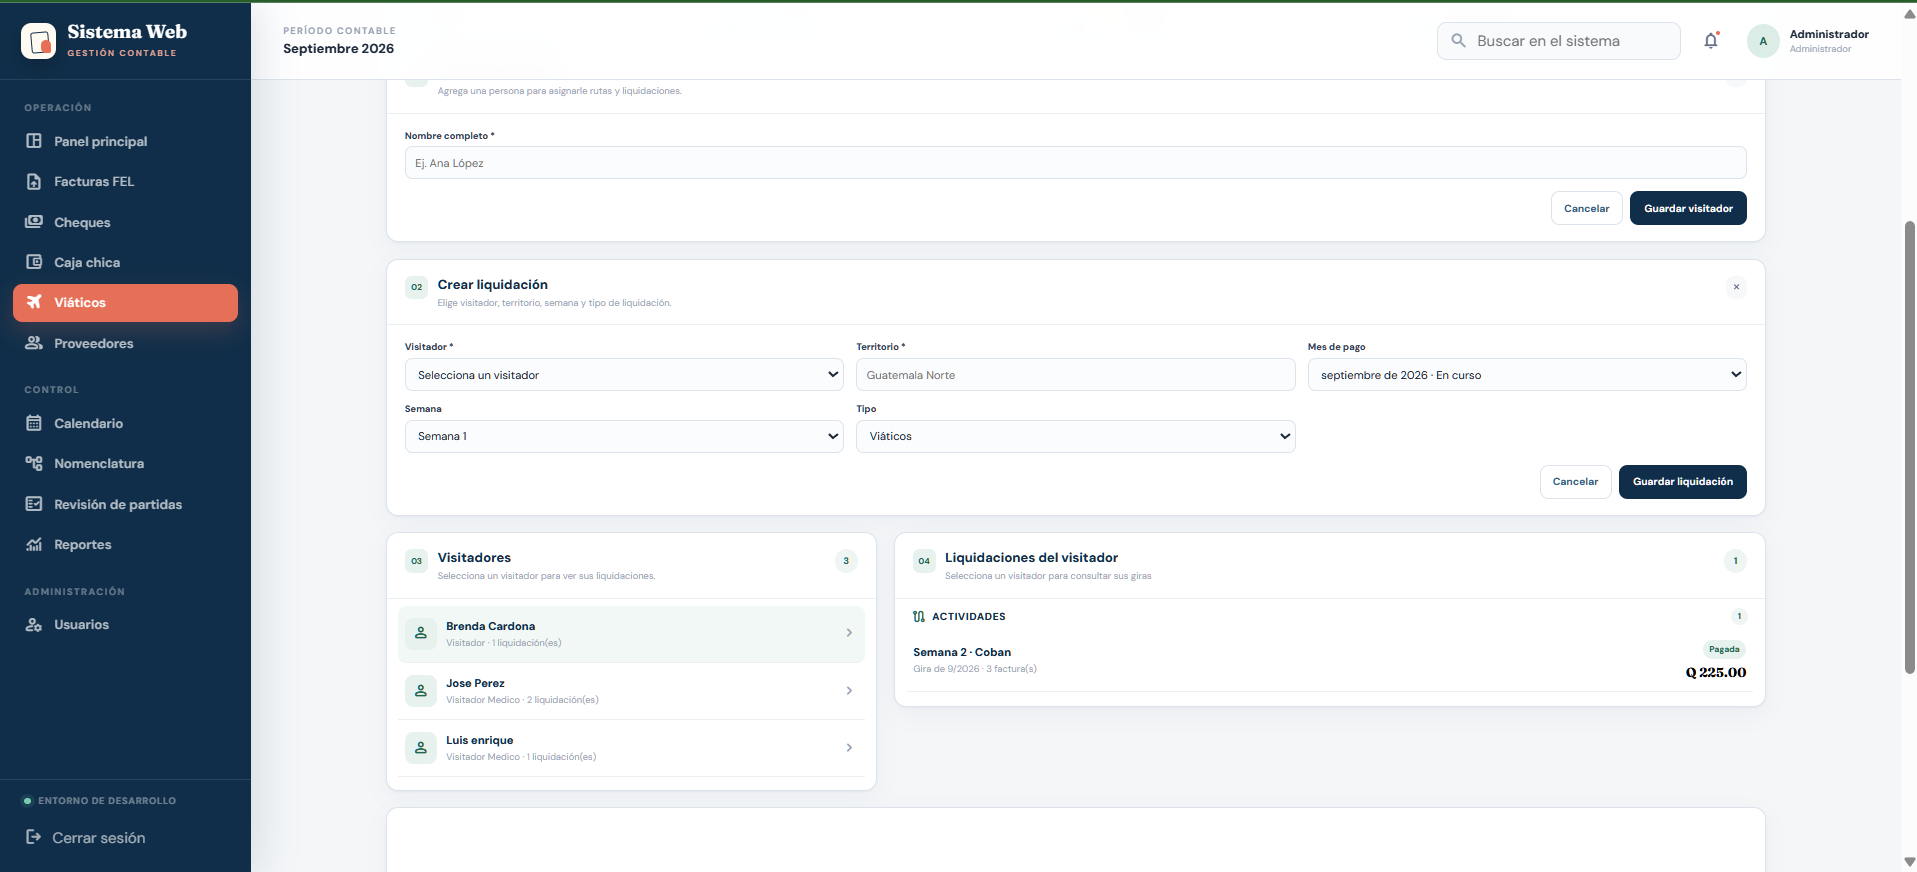
\includegraphics[width=0.96\linewidth]{capturas_reales/angular_actualizadas/pantalla_07_viaticos_nueva_liquidacion.png}
    \vspace{0.1cm}
    \begin{minipage}{0.96\linewidth}
        \small\textit{Nota.} Captura de la interfaz de asignación de viáticos operada bajo controles reactivos de TypeScript.
    \end{minipage}
\end{figure}

% =========================================================================
% FRAGMENTO 5: PROVEEDORES (PYTHON/FASTAPI)
% =========================================================================
\subsubsection{Fragmento 5: Alta de Proveedores y Asociación Contable}
\noindent\textbf{Módulo:} Proveedores \\
\textbf{Lenguaje:} Python (FastAPI)

A continuación, se presenta la función de creación de proveedores con verificación de formato tributario y asignación de cuenta por defecto:

\begin{minted}[breaklines, fontsize=\small]{python}
@router.post("/proveedores")
def registrar_proveedor(prov: ProveedorCreate, db: Session = Depends(get_db)):
    nit_existente = db.query(Proveedor).filter(Proveedor.nit == prov.nit).first()
    if nit_existente:
        raise HTTPException(status_code=400, detail="El NIT ingresado ya existe")
        
    cuenta = db.query(Nomenclatura).filter(Nomenclatura.id == prov.cuenta_nomenclatura_id).first()
    if not cuenta:
        raise HTTPException(status_code=404, detail="La cuenta contable especificada no existe")
        
    nuevo_prov = Proveedor(**prov.dict())
    db.add(nuevo_prov)
    db.commit()
    return nuevo_prov
\end{minted}

\noindent\textbf{Descripción:} Este código implementa la creación de registros maestros de proveedores. Verifica la singularidad del NIT registrado y corrobora la existencia de la cuenta en la Nomenclatura Contable previa a la grabación definitiva.

\begin{figure}[H]
    \centering
    \caption{Formulario de registro y cartera de crédito de proveedores.}
    \label{fig:cap4_code_proveedores}
    \vspace{0.2cm}
    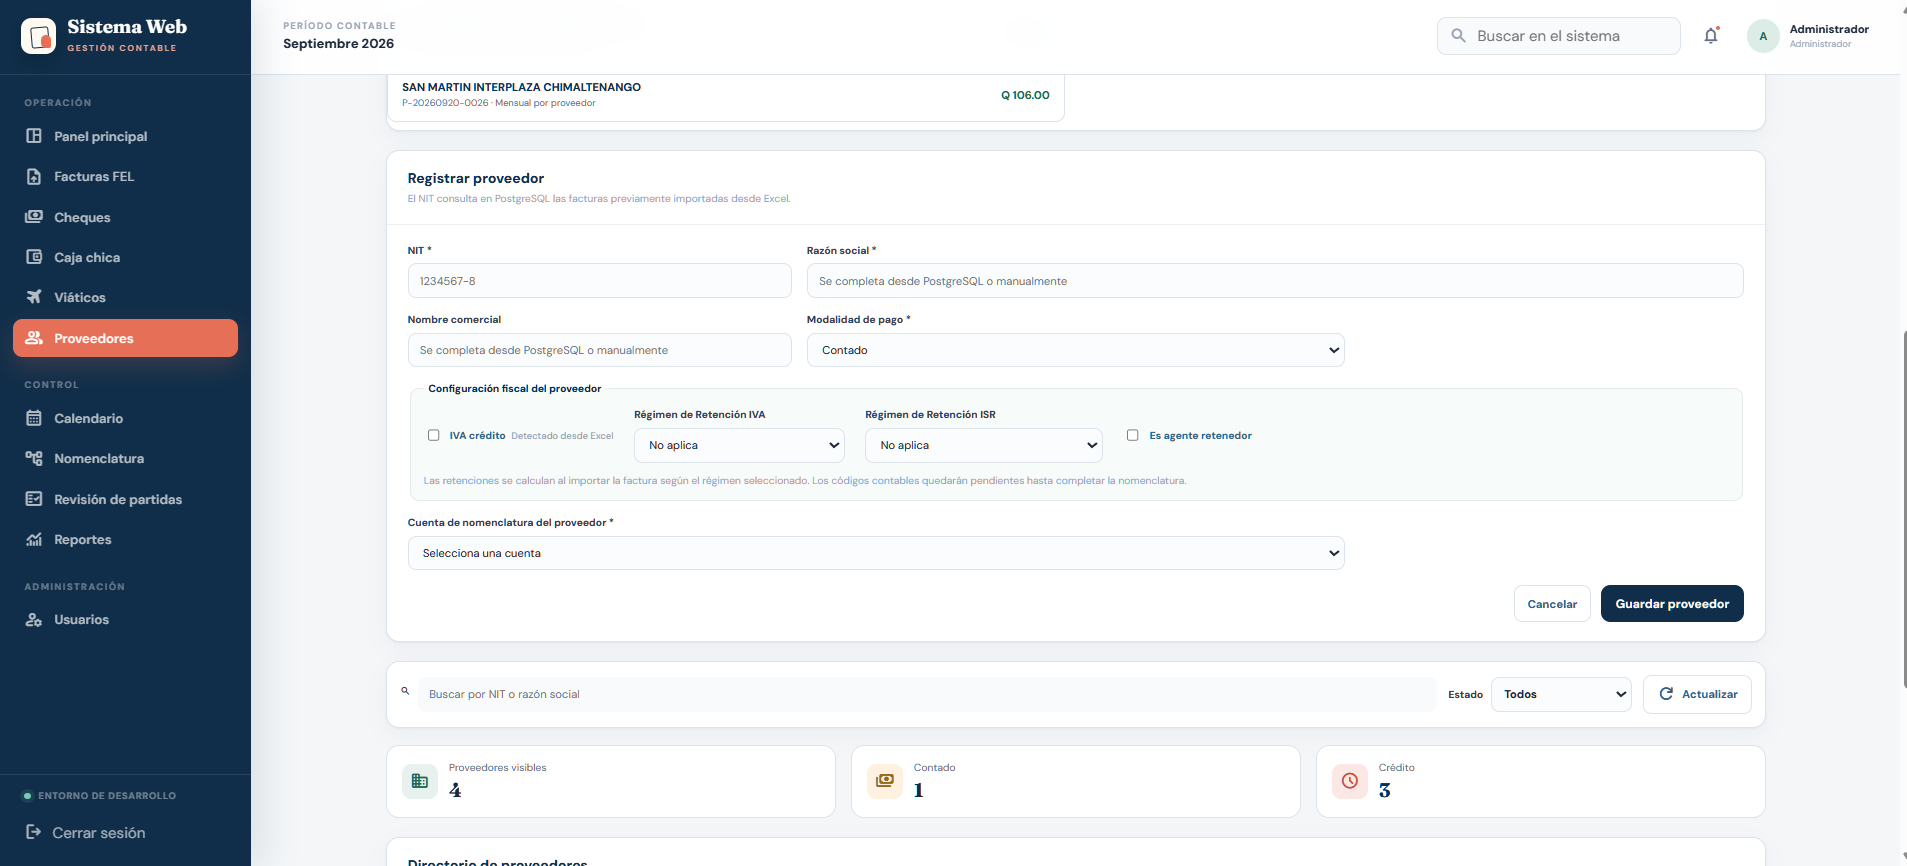
\includegraphics[width=0.96\linewidth]{capturas_reales/angular_actualizadas/pantalla_08_proveedores_nuevo.png}
    \vspace{0.1cm}
    \begin{minipage}{0.96\linewidth}
        \small\textit{Nota.} Formulario web interactivo que ejecuta la vinculación contable del proveedor respaldado en el código expuesto.
    \end{minipage}
\end{figure}

% =========================================================================
% FRAGMENTO 6: CALENDARIO OPERATIVO (TYPESCRIPT/ANGULAR)
% =========================================================================
\subsubsection{Fragmento 6: Programación Dinámica de Eventos Financieros}
\noindent\textbf{Módulo:} Calendario Operativo \\
\textbf{Lenguaje:} TypeScript (Angular)

A continuación, se expone el método del cliente que procesa la adición de eventos al calendario y renderiza la vista gráfica:

\begin{minted}[breaklines, fontsize=\small]{python}
agregarEventoCalendario(): void {
  if (this.eventoForm.invalid) {
    this.eventoForm.markAllAsTouched();
    return;
  }
  const nuevoEvento = this.eventoForm.value;
  this.calendarioService.guardarEvento(nuevoEvento).subscribe({
    next: (res) => {
      this.eventos.push(res);
      this.refrescarVistaCalendario();
      this.modalService.dismissAll();
    }
  });
}
\end{minted}

\noindent\textbf{Descripción:} El código pertenece al controlador frontend del Calendario Operativo. Valida el estado de los controles del formulario, envía la petición al backend y actualiza la lista de eventos renderizada en el componente dinámico.

\begin{figure}[H]
    \centering
    \caption{Vista de agenda y programación en el Calendario Operativo.}
    \label{fig:cap4_code_calendario}
    \vspace{0.2cm}
    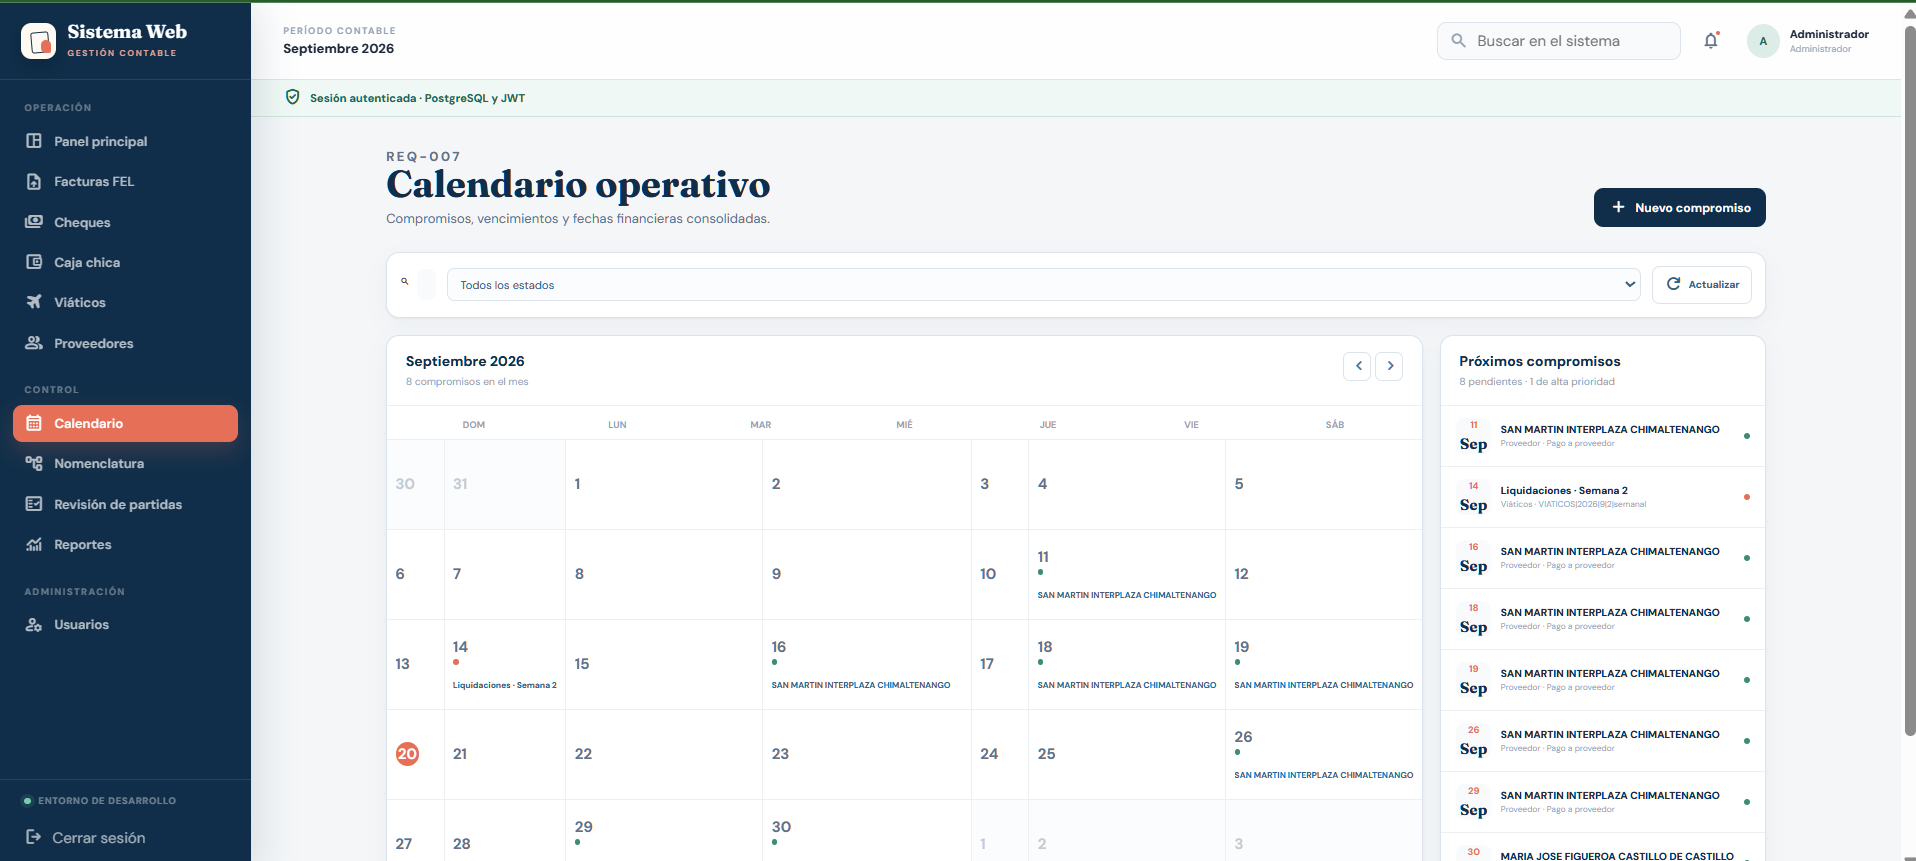
\includegraphics[width=0.96\linewidth]{capturas_reales/angular_actualizadas/pantalla_09_calendario.png}
    \vspace{0.1cm}
    \begin{minipage}{0.96\linewidth}
        \small\textit{Nota.} Pantalla operativa real del calendario que muestra la interacción directa con el script de gestión de eventos.
    \end{minipage}
\end{figure}

% =========================================================================
% FRAGMENTO 7: NOMENCLATURA CONTABLE (PYTHON/FASTAPI)
% =========================================================================
\subsubsection{Fragmento 7: Validación de Estructura de Cuentas Contables}
\noindent\textbf{Módulo:} Nomenclatura Contable \\
\textbf{Lenguaje:} Python (FastAPI)

A continuación, se detalla el fragmento encargado de validar el formato codificado jerárquico de las cuentas de catálogo:

\begin{minted}[breaklines, fontsize=\small]{python}
@router.post("/nomenclatura")
def crear_cuenta(cuenta: CuentaCreate, db: Session = Depends(get_db)):
    patron_codigo = r'^\d(\.\d+)*$'
    if not re.match(patron_codigo, cuenta.codigo_cuenta):
        raise HTTPException(status_code=400, detail="El formato del codigo contable es invalido")
        
    duplicado = db.query(Nomenclatura).filter(Nomenclatura.codigo == cuenta.codigo_cuenta).first()
    if duplicado:
        raise HTTPException(status_code=400, detail="El codigo contable ya fue registrado")
        
    nueva_cuenta = Nomenclatura(**cuenta.dict())
    db.add(nueva_cuenta)
    db.commit()
    return nueva_cuenta
\end{minted}

\noindent\textbf{Descripción:} El algoritmo evalúa el código contable propuesto mediante expresiones regulares para garantizar que cumpla con la notación por niveles (ejemplo: {5.1.01.001}) y confirma que no exista duplicidad jerárquica.

\begin{figure}[H]
    \centering
    \caption{Módulo de catálogo y mantenimiento de Nomenclatura Contable.}
    \label{fig:cap4_code_nomenclatura}
    \vspace{0.2cm}
    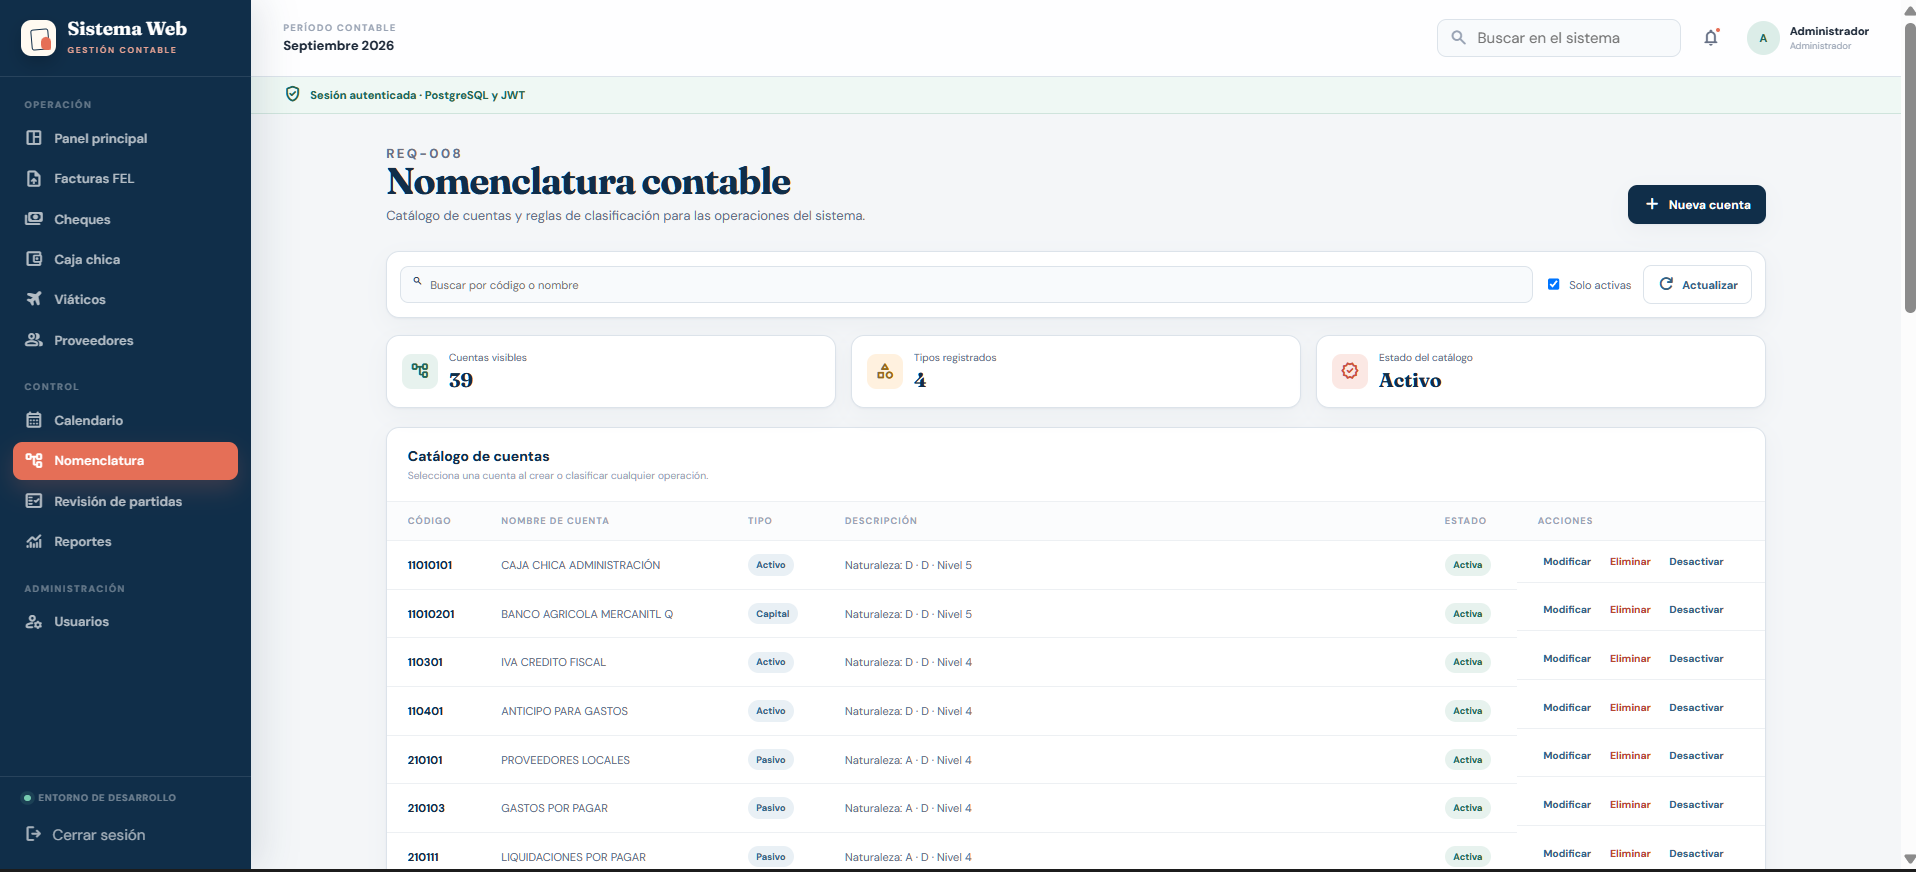
\includegraphics[width=0.96\linewidth]{capturas_reales/angular_actualizadas/pantalla_10_nomenclatura.png}
    \vspace{0.1cm}
    \begin{minipage}{0.96\linewidth}
        \small\textit{Nota.} Interfaz contable donde se administra el plan de cuentas mediante la lógica de validación jerárquica expuesta.
    \end{minipage}
\end{figure}

% =========================================================================
% FRAGMENTO 8: GESTIÓN DE USUARIOS (PYTHON/FASTAPI)
% =========================================================================
\subsubsection{Fragmento 8: Autenticación y Hashing de Credenciales}
\noindent\textbf{Módulo:} Gestión de Usuarios y Seguridad \\
\textbf{Lenguaje:} Python (FastAPI)

A continuación, se presenta un fragmento del procedimiento encargado de cifrar credenciales y dar de alta usuarios en la plataforma:

\begin{minted}[breaklines, fontsize=\small]{python}
@router.post("/usuarios")
def registrar_usuario(usuario: UsuarioCreate, db: Session = Depends(get_db)):
    email_existe = db.query(Usuario).filter(Usuario.email == usuario.email).first()
    if email_existe:
        raise HTTPException(status_code=400, detail="El correo electronico ya se encuentra registrado")
        
    password_hashed = pwd_context.hash(usuario.password)
    nuevo_usuario = Usuario(
        nombre=usuario.nombre,
        email=usuario.email,
        password_hash=password_hashed,
        rol_id=usuario.rol_id
    )
    db.add(nuevo_usuario)
    db.commit()
    return {"status": "exito", "mensaje": "Usuario creado correctamente"}
\end{minted}

\noindent\textbf{Descripción:} Este fragmento corresponde al componente de autenticación y seguridad del sistema. Recibe las credenciales, verifica la existencia del usuario y aplica el algoritmo de hashing seguro sobre la contraseña antes de validar la sesión.

\begin{figure}[H]
    \centering
    \caption{Pantalla de inicio de sesión asociada al proceso de autenticación y hashing.}
    \label{fig:cap4_code_usuarios}
    \vspace{0.2cm}
    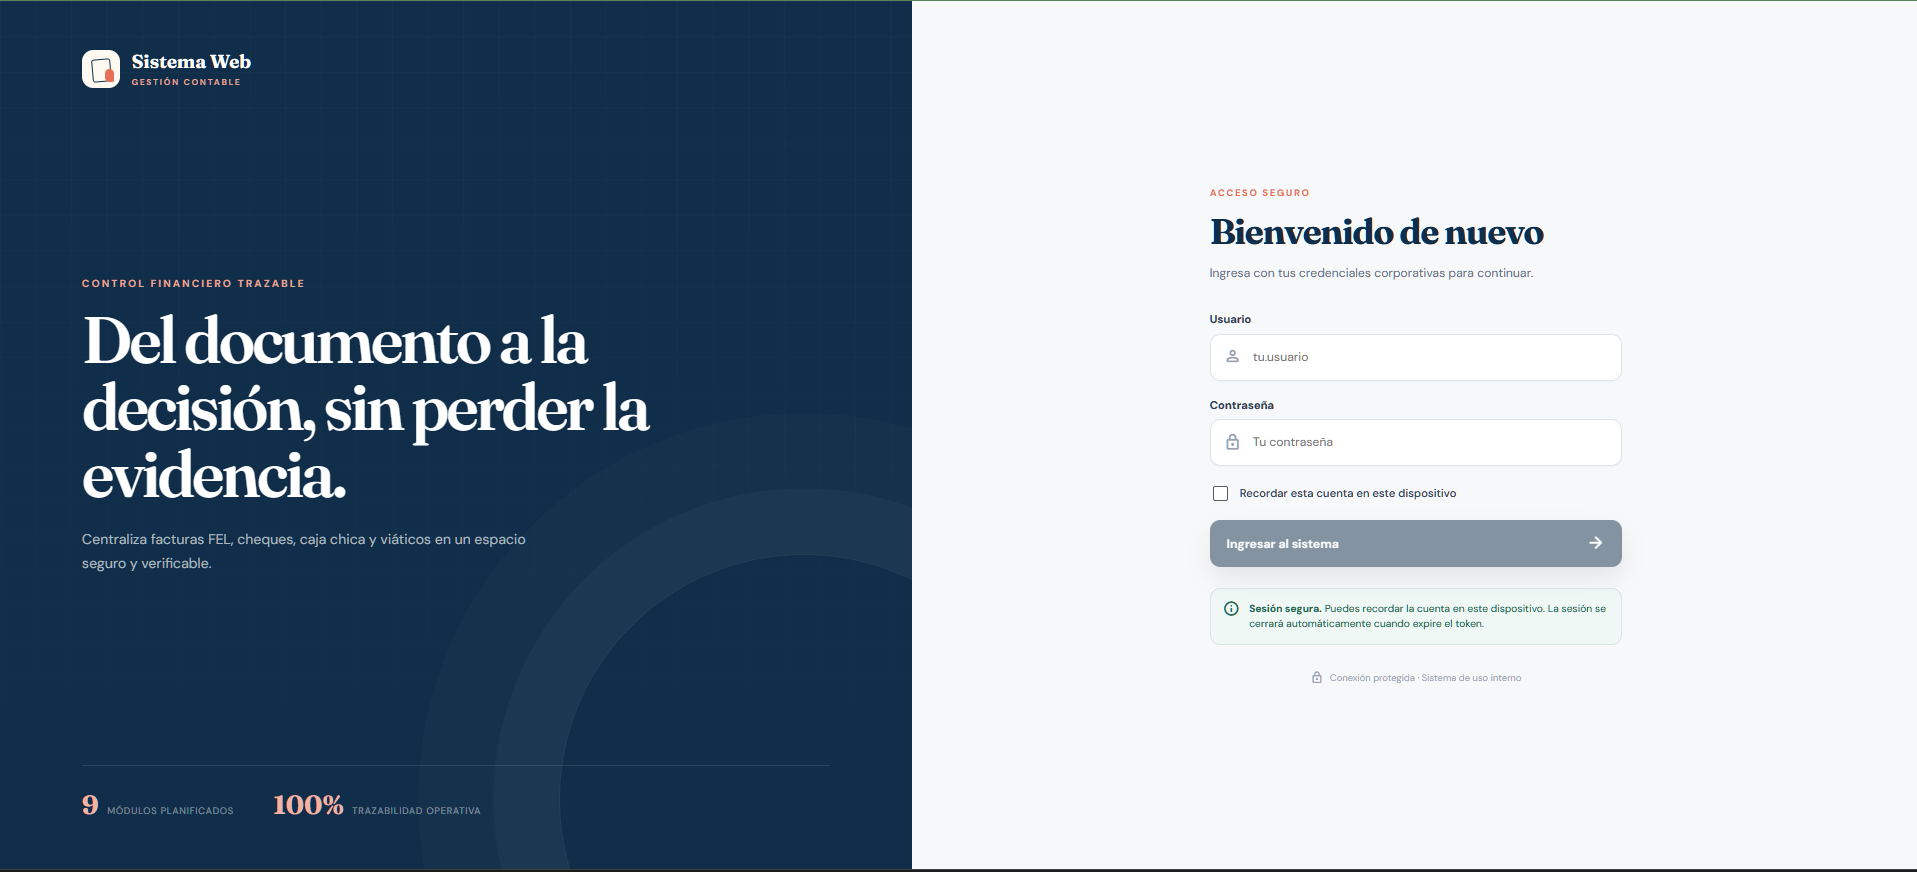
\includegraphics[width=0.96\linewidth]{capturas_reales/angular_actualizadas/pantalla_01_login.png}
    \vspace{0.1cm}
    \begin{minipage}{0.96\linewidth}
        \small\textit{Nota.} La captura corresponde a la interfaz de inicio de sesión relacionada con el proceso de autenticación y validación de credenciales.
    \end{minipage}
\end{figure}

\subsection{Objetos de la base de datos}
\label{sec:cap4_objetos_bd}

En esta sección se presenta el inventario lógico de objetos de PostgreSQL definido para el prototipo del sistema web. El inventario comprende tablas, procedimientos almacenados, vistas y disparadores (\textit{triggers}) relacionados con la integridad y automatización de los procesos contables.

\subsubsection{Listado de Tablas}

\setstretch{1.15}
\setlength{\parindent}{0pt}
\begin{xltabular}{\linewidth}{
    >{\raggedright\arraybackslash}p{3.8cm} 
    >{\raggedright\arraybackslash}X 
    >{\raggedright\arraybackslash}p{2.3cm} 
    >{\raggedright\arraybackslash}p{2.2cm}
}
    \caption{Listado de tablas principales del sistema de base de datos} \label{tab:cap4_bd_tablas} \\
    \toprule
    \textbf{Nombre de Tabla} & \textbf{Descripción de Contenido} & \textbf{Módulo} & \textbf{Llave Primaria} \\
    \midrule
    \endfirsthead

    \toprule
    \textbf{Nombre de Tabla} & \textbf{Descripción de Contenido} & \textbf{Módulo} & \textbf{Llave Primaria} \\
    \midrule
    \endhead

    \bottomrule
    \endfoot

    \bottomrule
    \endlastfoot

    {factura\_fel} & Registro maestro de comprobantes DTE autorizados por la SAT & Facturas FEL/SAT & {id} (UUID) \\
    \addlinespace
    {cheque\_posfechado} & Control de cheques recibidos, fechas de cobro y estados & Cheques Posfechados & {id} (BIGINT) \\
    \addlinespace
    {fondo\_caja\_chica} & Administración de los fondos fijos autorizados & Caja Chica & {id} (INTEGER) \\
    \addlinespace
    {movimiento\_caja} & Registro de vales, recibos y egresos de caja chica & Caja Chica & {id} (BIGINT) \\
    \addlinespace
    {gira\_viatico} & Control de asignación de giras semanales y colaboradores & Viáticos & {id} (INTEGER) \\
    \addlinespace
    {proveedor} & Expediente maestro de proveedores y cuentas por pagar & Proveedores & {id} (INTEGER) \\
    \addlinespace
    {evento\_calendario} & Programación de vencimientos, giras y fechas de depósito & Calendario Operativo & {id} (BIGINT) \\
    \addlinespace
    {nomenclatura\_cuenta} & Plan maestro de cuentas jerárquicas y estructura contable & Nomenclatura & {id} (INTEGER) \\
    \addlinespace
    {usuario} & Registro de usuarios, credenciales y asignación de roles & Seguridad & {id} (INTEGER) \\

\end{xltabular}

\subsubsection{Listado de Procedimientos Almacenados}

{
\small
\setstretch{1.15}
\setlength{\parindent}{0pt}
\begin{xltabular}{\linewidth}{
    >{\raggedright\arraybackslash}p{3.5cm} 
    >{\raggedright\arraybackslash}>{\hsize=1.15\hsize}X 
    >{\raggedright\arraybackslash}>{\hsize=0.85\hsize}X
}
    \caption{Listado de procedimientos almacenados del sistema} \label{tab:cap4_bd_sp} \\
    \toprule
    \textbf{Procedimiento Almacenado} & \textbf{Propósito / Función Operativa} & \textbf{Parámetros Principales} \\
    \midrule
    \endfirsthead

    \toprule
    \textbf{Procedimiento Almacenado} & \textbf{Propósito / Función Operativa} & \textbf{Parámetros Principales} \\
    \midrule
    \endhead

    \bottomrule
    \endfoot

    \bottomrule
    \endlastfoot

    {sp\_liquidar\_caja\_chica} & Consolida los movimientos vigentes de caja chica y genera el asiento contable de liquidación & {p\_fondo\_id}, {p\_usuario\_id} \\
    \addlinespace
    {sp\_asignar\_factura\_gira} & Vincula comprobantes a giras operativas validando límites semanales por categoría & {p\_gira\_id}, {p\_factura\_id}, {p\_categoria} \\
    \addlinespace
    {sp\_procesar\_carga\_fel} & Inserta masivamente facturas validadas desde archivos XML evitando duplicidad de UUID & {p\_xml\_data}, {p\_usuario\_id} \\
    \addlinespace
    {sp\_generar\_cierre\_mes} & Efectúa el balance mensual de sumas y saldos bloqueando modificaciones al período contable & {p\_anio}, {p\_mes} \\

\end{xltabular}
}

\subsubsection{Listado de Vistas}

{
\small
\setstretch{1.15}
\setlength{\parindent}{0pt}
\begin{xltabular}{\linewidth}{
    >{\raggedright\arraybackslash}p{3.5cm} 
    >{\raggedright\arraybackslash}X 
    >{\raggedright\arraybackslash}p{2.5cm}
}
    \caption{Listado de vistas para consultas y reportes del sistema} \label{tab:cap4_bd_vistas} \\
    \toprule
    \textbf{Nombre de la Vista} & \textbf{Descripción / Consulta Representada} & \textbf{Módulo Asociado} \\
    \midrule
    \endfirsthead

    \toprule
    \textbf{Nombre de la Vista} & \textbf{Descripción / Consulta Representada} & \textbf{Módulo Asociado} \\
    \midrule
    \endhead

    \bottomrule
    \endfoot

    \bottomrule
    \endlastfoot

    {vw\_estado\_cheques} & Resumen consolidado de cheques cobrados, pendientes y rechazados con totales por banco & Cheques Posfechados \\
    \addlinespace
    {vw\_arqueo\_caja\_chica} & Arqueo en tiempo real indicando asignación inicial, egresos acumulados y disponible & Caja Chica \\
    \addlinespace
    {vw\_cartera\_proveedores} & Estado de cuenta por proveedor detallando saldo vencido y crédito disponible & Proveedores \\
    \addlinespace
    {vw\_balance\_comprobacion} & Vista acumulativa del saldo deudor y acreedor por cuenta de nomenclatura contable & Reportes \\

\end{xltabular}
}

\subsubsection{Listado de Triggers (Disparadores)}

{
\small
\setstretch{1.15}
\setlength{\parindent}{0pt}
\begin{xltabular}{\linewidth}{
    >{\raggedright\arraybackslash}p{3.2cm} 
    >{\raggedright\arraybackslash}p{2.8cm} 
    >{\raggedright\arraybackslash}X
}
    \caption{Listado de triggers para control de reglas de negocio e integridad} \label{tab:cap4_bd_triggers} \\
    \toprule
    \textbf{Nombre del Trigger} & \textbf{Tabla y Evento} & \textbf{Regla de Negocio / Función Automatizada} \\
    \midrule
    \endfirsthead

    \toprule
    \textbf{Nombre del Trigger} & \textbf{Tabla y Evento} & \textbf{Regla de Negocio / Función Automatizada} \\
    \midrule
    \endhead

    \bottomrule
    \endfoot

    \bottomrule
    \endlastfoot

    {trg\_actualiza\_saldo\_caja} & {movimiento\_caja} (AFTER INSERT) & Descuenta automáticamente el valor del recibo registrado del saldo disponible del fondo fijo. \\
    \addlinespace
    {trg\_valida\_fecha\_cheque} & {cheque\_posfechado} (BEFORE INSERT/UPDATE) & Impide la grabación si la fecha de depósito es anterior a la fecha de emisión o recepción. \\
    \addlinespace
    {trg\_auditoria\_nomenclatura} & {nomenclatura\_cuenta} (AFTER UPDATE/DELETE) & Registra en la tabla de auditoría cualquier cambio estructurado o eliminación en el plan de cuentas. \\

\end{xltabular}
}

\subsubsection{Esquema Entidad-Relación (Diagrama E-R)}

A continuación, se presenta el esquema relacional documentado para los módulos del sistema, ilustrando las relaciones, llaves primarias y llaves foráneas consideradas en el diseño.

\begin{figure}[H]
    \centering
    \caption{Esquema Entidad-Relación del modelo de base de datos relacional.}
    \label{fig:cap4_diagrama_er}
    \vspace{0.2cm}
    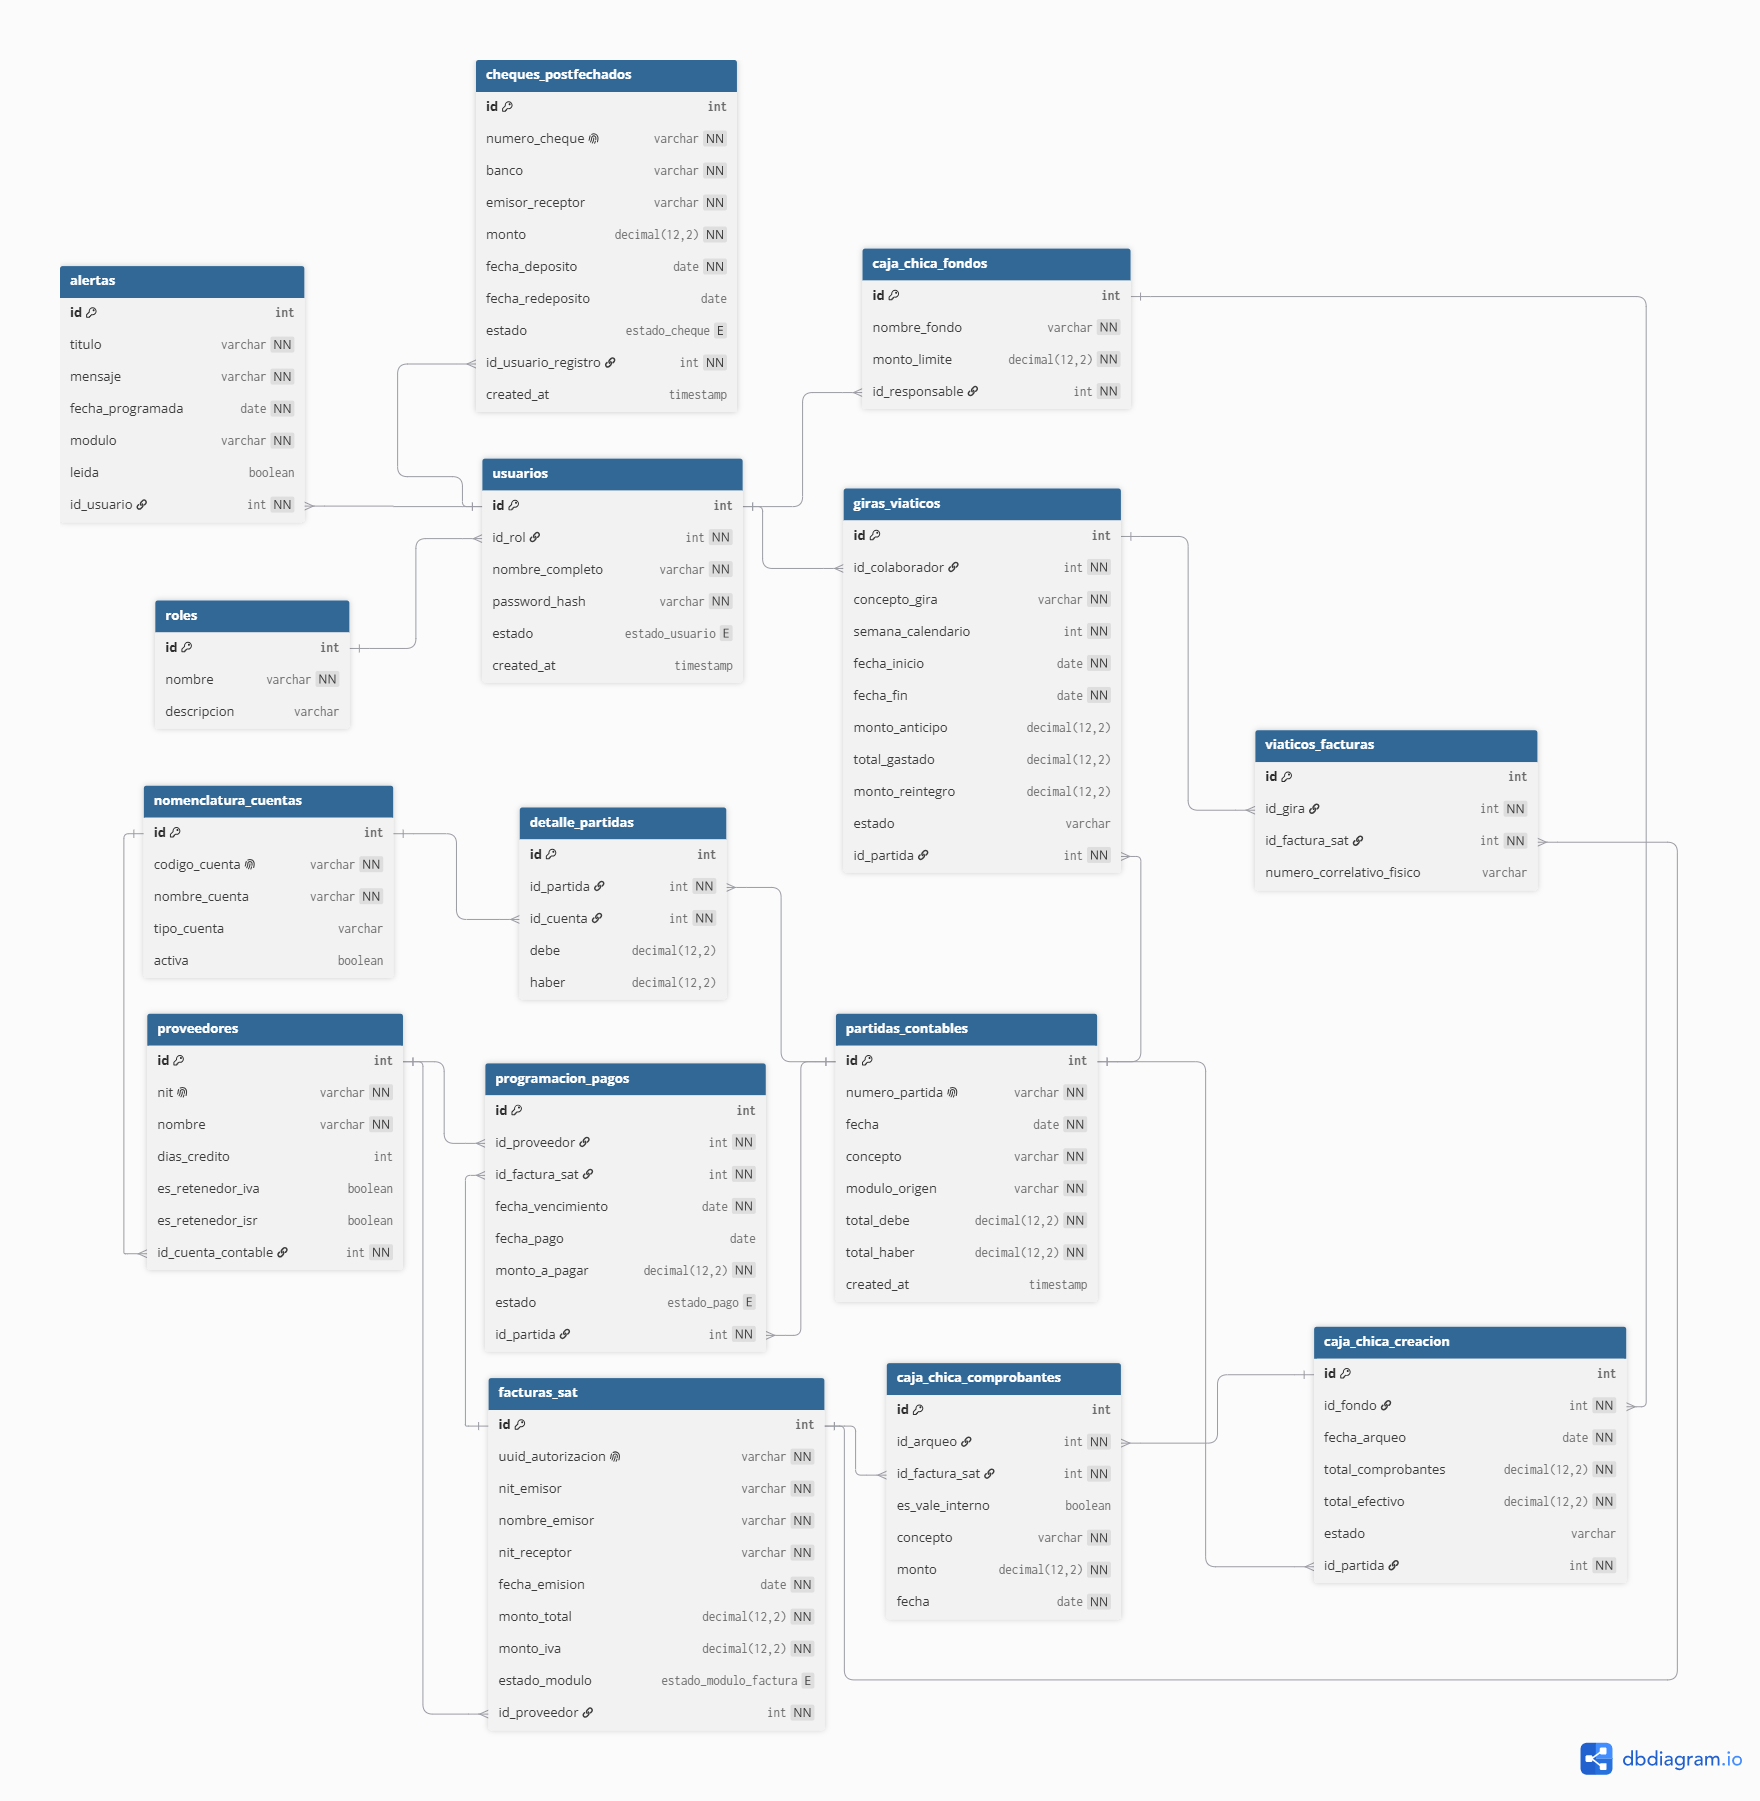
\includegraphics[width=0.96\linewidth]{imagenes/diagramabd.png}
    \vspace{0.1cm}
    \begin{minipage}{0.96\linewidth}
        \small El diagrama representa la estructura relacional utilizada como referencia para la implementación del prototipo.
    \end{minipage}
\end{figure}

\subsection{ Pruebas Realizadas}
\label{sec:cap4_pruebas_realizadas}

La validación funcional se realizó sobre el prototipo actual del sistema en los módulos de Facturas FEL/SAT, Proveedores y Nomenclatura contable. Se evaluaron diez aspectos directamente en el navegador autenticado, utilizando las vistas, registros y controles disponibles al momento de la prueba. Los resultados se clasifican como \textit{Aprobado} cuando la acción produjo un resultado observable, \textit{No verificable} cuando el control no produjo una respuesta visible y \textit{No ejecutado} cuando faltó un dato de entrada necesario.

Los resultados corresponden a la ejecución real del prototipo en el entorno local. Por consiguiente, no se presenta una efectividad del cien por ciento ni se extrapolan estos datos a un ambiente productivo.

\paragraph{Clasificación de las pruebas}
Las pruebas unitarias (U) verifican una validación o regla aislada. Las pruebas de integración (INT) comprueban el intercambio de información entre componentes. Las pruebas de sistema (SIS) recorren una operación completa del módulo. Las pruebas de aceptación (ACEP) verifican que el flujo satisfaga la necesidad operativa definida.

\subsubsection{Módulo de Facturas}
{
\fontsize{8}{10}\selectfont
\setstretch{1.15}
\setlength{\parindent}{0pt}
\setlength{\tabcolsep}{3pt}

\begin{xltabular}{\linewidth}{
    l                                     % ID
    >{\raggedright\arraybackslash}p{1.2cm} % Módulo
    >{\raggedright\arraybackslash}p{1.3cm} % Tipo
    >{\raggedright\arraybackslash}p{1.6cm} % Caso
    >{\raggedright\arraybackslash}p{1.4cm} % Datos
    >{\raggedright\arraybackslash}X       % Pasos
    >{\raggedright\arraybackslash}X       % Esperado
    >{\raggedright\arraybackslash}X       % Obtenido
    c                                     % Estado
}
\caption{Casos de prueba del módulo de Facturas FEL/SAT}\label{tab:cap4_pruebas_fel_actualizadas}\\
\toprule
\textbf{ID} & \textbf{Módulo} & \textbf{Tipo} & \textbf{Caso} & \textbf{Datos} & \textbf{Pasos} & \textbf{Esperado} & \textbf{Obtenido} & \textbf{Estado}\\
\midrule
\endfirsthead

\toprule
\textbf{ID} & \textbf{Módulo} & \textbf{Tipo} & \textbf{Caso} & \textbf{Datos} & \textbf{Pasos} & \textbf{Esperado} & \textbf{Obtenido} & \textbf{Estado}\\
\midrule
\endhead

\bottomrule
\endfoot

\bottomrule
\endlastfoot

FEL-01 & FEL & SIS & Acceso y disponibilidad & -- & Iniciar sesión y navegar a Facturas FEL. & El módulo carga y permite consultar sus controles. & La vista cargó correctamente con el mensaje ``POSTGRESQL CONECTADO''. & OK\\
\addlinespace
FEL-02 & FEL & SIS & Consulta histórica & -- & Presionar ``Mostrar datos cargados''. & Debe aparecer el catálogo histórico de DTEs. & Se desplegó el listado con UUID, emisor y montos cargados. & OK\\
\addlinespace
FEL-03 & FEL & SIS & Carga de archivo & Archivo XLSX & Seleccionar un archivo de hasta 15 MB y procesar. & El archivo debe ser procesado e ingresado a la BD. & Respuesta exitosa HTTP 200 OK y registro correcto en base de datos. & OK\\
\addlinespace
FEL-04 & FEL & SIS & Validaciones previas & Archivo FEL válido & Revisar el bloque de validación antes del procesamiento. & Deben validarse receptor, NIT, autorización e IVA. & Se ejecutaron las validaciones de datos emitiendo estado verificado. & OK\\
\addlinespace
FEL-05 & FEL & SIS & Control de duplicados & XML con UUID duplicado & Intentar subir un DTE previamente registrado. & Denegar el procesamiento y notificar duplicidad. & El sistema rechazó la carga mostrando alerta de DTE duplicado. & OK\\
\addlinespace
FEL-06 & FEL & SIS & Inconsistencia de montos & DTE con monto cero & Procesar DTE con valor numérico no válido. & Bloquear carga y mostrar advertencia de inconsistencia. & El sistema procesó la factura sin emitir advertencia por el monto cero. & No OK\\
\end{xltabular}
}

{
\small
\setstretch{1.15}
\setlength{\parindent}{0pt}
\begin{xltabular}{\linewidth}{
    >{\raggedright\arraybackslash}p{2.5cm} 
    >{\raggedright\arraybackslash}X 
    >{\centering\arraybackslash}p{1.4cm} 
    >{\centering\arraybackslash}p{1.4cm} 
    >{\centering\arraybackslash}p{1.5cm}
}
\caption{Resultados numéricos del módulo de Facturas FEL/SAT}\label{tab:cap4_metricas_fel_actualizadas}\tabularnewline
\toprule
\textbf{Métrica} & \textbf{Definición} & \textbf{Casos evaluados} & \textbf{Casos aprobados} & \textbf{Resultado}\\
\midrule
\endfirsthead
\toprule
\textbf{Métrica} & \textbf{Definición} & \textbf{Casos evaluados} & \textbf{Casos aprobados} & \textbf{Resultado}\\
\midrule
\endhead
\bottomrule
\endfoot
\bottomrule
\endlastfoot
Efectividad observable & Casos aprobados / casos evaluados $\times 100$. & 6 & 5 & 83.3\%\\
\end{xltabular}
}

\begin{figure}[H]
\centering
\caption{Resultado observado de pruebas del módulo de Facturas FEL/SAT.}\label{fig:cap4_grafica_fel_actualizada}
\begin{tikzpicture}
\begin{axis}[ybar,width=0.78\linewidth,height=5.3cm,ymin=0,ymax=100,ylabel={Porcentaje de aprobación},symbolic x coords={FEL},xtick=data,nodes near coords,bar width=1.2cm,ymajorgrids=true,grid style=dashed]
\addplot[fill=blue!65] coordinates {(FEL,83.3)};
\end{axis}
\end{tikzpicture}
\end{figure}

\noindent\textbf{Interpretación:} El módulo de Facturas FEL/SAT obtuvo un 83.3\% de efectividad. Se confirmaron de forma satisfactoria la disponibilidad del módulo, la consulta histórica, la carga de archivos, las validaciones de estructura y la detección de duplicados. Únicamente se observó un fallo al no reaccionar ante una inconsistencia en el monto del comprobante.

\subsubsection{Módulo de Proveedores}

Se evaluaron cinco aspectos del módulo. Se verificaron correctamente la consulta del catálogo, la modificación del tipo de partida, la creación de nuevos proveedores y la búsqueda por NIT. La generación de partidas transitorias no mostró una respuesta visible en pantalla.

{
\fontsize{8}{10}\selectfont
\setstretch{1.15}
\setlength{\parindent}{0pt}
\setlength{\tabcolsep}{3pt}

\begin{xltabular}{\linewidth}{
    l                                     % ID
    >{\raggedright\arraybackslash}p{1.2cm} % Módulo
    >{\raggedright\arraybackslash}p{1.3cm} % Tipo
    >{\raggedright\arraybackslash}p{1.6cm} % Caso
    >{\raggedright\arraybackslash}p{1.4cm} % Datos
    >{\raggedright\arraybackslash}X       % Pasos
    >{\raggedright\arraybackslash}X       % Esperado
    >{\raggedright\arraybackslash}X       % Obtenido
    c                                     % Estado
}
\caption{Casos de prueba del módulo de Proveedores}\label{tab:cap4_pruebas_proveedores_actualizadas}\tabularnewline
\toprule
\textbf{ID} & \textbf{Módulo} & \textbf{Tipo} & \textbf{Caso} & \textbf{Datos} & \textbf{Pasos} & \textbf{Esperado} & \textbf{Obtenido} & \textbf{Estado}\\
\midrule
\endfirsthead
\toprule
\textbf{ID} & \textbf{Módulo} & \textbf{Tipo} & \textbf{Caso} & \textbf{Datos} & \textbf{Pasos} & \textbf{Esperado} & \textbf{Obtenido} & \textbf{Estado}\\
\midrule
\endhead
\bottomrule
\endfoot
\bottomrule
\endlastfoot
PROV-01 & Proveedores & SIS & Consulta del directorio & -- & Abrir módulo y revisar datos, crédito y cuentas. & El directorio debe mostrar los registros. & Se visualizaron los proveedores activos con sus respectivas condiciones. & OK\\
\addlinespace
PROV-02 & Proveedores & SIS & Modalidad de partida & -- & Cambiar ``Tipo de partida'' a ``Transitoria''. & Ajustar la modalidad de generación. & La interfaz actualizó la modalidad ocultando campos no requeridos. & OK\\
\addlinespace
PROV-03 & Proveedores & SIS & Registro de proveedor & Datos de proveedor & Llenar formulario y presionar ``Guardar''. & Crear el nuevo proveedor en el sistema. & El proveedor se guardó con éxito y apareció en el directorio general. & OK\\
\addlinespace
PROV-04 & Proveedores & SIS & Búsqueda por NIT & NIT válido & Ingresar número de NIT en el filtro. & Filtrar la lista por el proveedor solicitado. & La tabla se actualizó mostrando únicamente el proveedor coincidente. & OK\\
\addlinespace
PROV-05 & Proveedores & SIS & Generación de partida & -- & Presionar ``Generar partidas'' transitorias. & Mostrar mensaje de confirmación o partida. & El botón recibió la interacción, pero no se observó un resultado nuevo en la vista. & No OK\\
\end{xltabular}
}

{
\small
\setstretch{1.15}
\setlength{\parindent}{0pt}
\begin{xltabular}{\linewidth}{
    >{\raggedright\arraybackslash}p{2.5cm} 
    >{\raggedright\arraybackslash}X 
    >{\centering\arraybackslash}p{1.4cm} 
    >{\centering\arraybackslash}p{1.4cm} 
    >{\centering\arraybackslash}p{1.5cm}
}
\caption{Resultados numéricos del módulo de Proveedores}\label{tab:cap4_metricas_proveedores_actualizadas}\tabularnewline
\toprule
\textbf{Métrica} & \textbf{Definición} & \textbf{Casos evaluados} & \textbf{Casos aprobados} & \textbf{Resultado}\\
\midrule
\endfirsthead
\toprule
\textbf{Métrica} & \textbf{Definición} & \textbf{Casos evaluados} & \textbf{Casos aprobados} & \textbf{Resultado}\\
\midrule
\endhead
\bottomrule
\endfoot
\bottomrule
\endlastfoot
Efectividad observable & Casos aprobados / casos evaluados $\times 100$. & 5 & 4 & 80.0\%\\
\end{xltabular}
}

\begin{figure}[H]
\centering
\caption{Resultado observado de pruebas del módulo de Proveedores.}\label{fig:cap4_grafica_proveedores_actualizada}
\begin{tikzpicture}
\begin{axis}[ybar,width=0.78\linewidth,height=5.3cm,ymin=0,ymax=100,ylabel={Porcentaje de aprobación},symbolic x coords={Proveedores},xtick=data,nodes near coords,bar width=1.2cm,ymajorgrids=true,grid style=dashed]
\addplot[fill=green!55!black] coordinates {(Proveedores,80.0)};
\end{axis}
\end{tikzpicture}
\end{figure}

\noindent\textbf{Interpretación:} El módulo de Proveedores alcanzó un 80.0\% de efectividad observable. Fueron aprobadas las consultas, la modalidad de partidas, la creación y búsqueda de registros. Únicamente la generación de partidas transitorias quedó sin confirmar debido a la falta de respuesta visual en la pantalla.

\subsubsection{Módulo de Nomenclatura Contable}

Se evaluaron cinco aspectos del módulo. La carga del catálogo, las búsquedas por código, los filtros por naturaleza contable y la exportación de información operaron correctamente. La apertura del formulario de creación de nuevas cuentas presentó un fallo de interfaz.

{
\fontsize{8}{10}\selectfont
\setstretch{1.15}
\setlength{\parindent}{0pt}
\setlength{\tabcolsep}{3pt}

\begin{xltabular}{\linewidth}{
    l                                     % ID
    >{\raggedright\arraybackslash}p{1.2cm} % Módulo
    >{\raggedright\arraybackslash}p{1.3cm} % Tipo
    >{\raggedright\arraybackslash}p{1.6cm} % Caso
    >{\raggedright\arraybackslash}p{1.4cm} % Datos
    >{\raggedright\arraybackslash}X       % Pasos
    >{\raggedright\arraybackslash}X       % Esperado
    >{\raggedright\arraybackslash}X       % Obtenido
    c                                     % Estado
}
\caption{Casos de prueba del módulo de Nomenclatura contable}\label{tab:cap4_pruebas_nomenclatura_actualizadas}\tabularnewline
\toprule
\textbf{ID} & \textbf{Módulo} & \textbf{Tipo} & \textbf{Caso} & \textbf{Datos} & \textbf{Pasos} & \textbf{Esperado} & \textbf{Obtenido} & \textbf{Estado}\\
\midrule
\endfirsthead
\toprule
\textbf{ID} & \textbf{Módulo} & \textbf{Tipo} & \textbf{Caso} & \textbf{Datos} & \textbf{Pasos} & \textbf{Esperado} & \textbf{Obtenido} & \textbf{Estado}\\
\midrule
\endhead
\bottomrule
\endfoot
\bottomrule
\endlastfoot
NOM-01 & Nomenclatura & SIS & Carga del catálogo & -- & Abrir módulo y consultar indicadores. & Cargar catálogo de cuentas completo. & Se visualizaron 39 cuentas registradas y estado ``Activo''. & OK\\
\addlinespace
NOM-02 & Nomenclatura & SIS & Búsqueda por código & Código: 610112 & Ingresar el código en el buscador. & Mostrar la cuenta correspondiente. & Se filtró a la cuenta ``DEPRECIACIONES Y COMBUSTIBLES'' correctamente. & OK\\
\addlinespace
NOM-03 & Nomenclatura & SIS & Filtro por naturaleza & Tipo: Gasto & Seleccionar filtro por tipo de cuenta. & Mostrar únicamente cuentas de gasto. & La lista se actualizó correctamente con el grupo de cuentas solicitado. & OK\\
\addlinespace
NOM-04 & Nomenclatura & SIS & Exportación de catálogo & -- & Presionar botón ``Exportar a Excel''. & Generar archivo comprimido o hoja de cálculo. & Se descargó el archivo XLSX con la estructura contable completa. & OK\\
\addlinespace
NOM-05 & Nomenclatura & SIS & Nueva cuenta & -- & Presionar botón ``Nueva cuenta''. & Desplegar formulario de registro. & El botón recibió la interacción, pero no abrió un formulario visible. & No OK\\
\end{xltabular}
}

{
\small
\setstretch{1.15}
\setlength{\parindent}{0pt}
\begin{xltabular}{\linewidth}{
    >{\raggedright\arraybackslash}p{2.5cm} 
    >{\raggedright\arraybackslash}X 
    >{\centering\arraybackslash}p{1.4cm} 
    >{\centering\arraybackslash}p{1.4cm} 
    >{\centering\arraybackslash}p{1.5cm}
}
\caption{Resultados numéricos del módulo de Nomenclatura contable}\label{tab:cap4_metricas_nomenclatura_actualizadas}\tabularnewline
\toprule
\textbf{Métrica} & \textbf{Definición} & \textbf{Casos evaluados} & \textbf{Casos aprobados} & \textbf{Resultado}\\
\midrule
\endfirsthead
\toprule
\textbf{Métrica} & \textbf{Definición} & \textbf{Casos evaluados} & \textbf{Casos aprobados} & \textbf{Resultado}\\
\midrule
\endhead
\bottomrule
\endfoot
\bottomrule
\endlastfoot
Efectividad observable & Casos aprobados / casos evaluados $\times 100$. & 5 & 4 & 80.0\%\\
\end{xltabular}
}

\begin{figure}[H]
\centering
\caption{Resultado observado de pruebas del módulo de Nomenclatura contable.}\label{fig:cap4_grafica_nomenclatura_actualizada}
\begin{tikzpicture}
\begin{axis}[ybar,width=0.78\linewidth,height=5.3cm,ymin=0,ymax=100,ylabel={Porcentaje de aprobación},symbolic x coords={Nomenclatura},xtick=data,nodes near coords,bar width=1.2cm,ymajorgrids=true,grid style=dashed]
\addplot[fill=orange!80!black] coordinates {(Nomenclatura,80.0)};
\end{axis}
\end{tikzpicture}
\end{figure}

\noindent\textbf{Interpretación:} El módulo de Nomenclatura Contable registró un 80.0\% de efectividad observable. La consulta de información, búsquedas, filtrados y la exportación de datos funcionaron con normalidad. Solo se identificó una inconsistencia en la apertura del formulario para registrar nuevas cuentas.

\paragraph{Resumen de la ejecución}
En conjunto se evaluaron 16 casos de prueba: seis en Facturas FEL/SAT, cinco en Proveedores y cinco en Nomenclatura contable. Se obtuvieron 13 casos aprobados y 3 casos no verificados o con falla. La efectividad observable global fue de 13 casos aprobados sobre 16 evaluados, equivalente al 81.3\%. Este resultado refleja un nivel adecuado de estabilidad funcional durante la fase de validación del prototipo.
\include{capitulos/Cap_V_anlisis_resultados}
\section*{Conclusiones}\label{conclusiones}
\addcontentsline{toc}{section}{Conclusiones}

Se redacta una por cada objetivo específico, lo que significa que deben
ser al menos cinco, y se debe aplicar el mismo orden de los objetivos
específicos.

\newpage

\section*{Recomendaciones}\label{recomendaciones}
\addcontentsline{toc}{section}{Recomendaciones}

Debe incluir todo lo que recomienda para que el proyecto funcione
correctamente, por ejemplo:

\begin{itemize}
\item
  Se recomienda realizar backups periódicamente
\item
  Se recomienda utilizar antivirus en los servidores como en las
  computadoras cliente
\item
  Renovación de licencias, entre otros
\end{itemize}

\newpage
\section*{Bibliografía} % APA 7 pide que se llame Referencias, no Bibliografía
\addcontentsline{toc}{section}{Referencias} % Para que aparezca en el índice

\begingroup
\setlength{\parindent}{0pt}
\setlength{\parskip}{0.5cm} % Aquí está la separación visual que pediste
\everypar{\hangindent=1.27cm\relax} % La sangría francesa oficial

American Institute of Certified Public Accountants (AICPA). (1961). \emph{Accounting Terminology Bulletins, No. 1: Review and Résumé}.

Arellano Rodríguez, M. (2008). \emph{Sistemas de información: ¿adecuación a los cambios tecnológicos o herramienta de gestión? Revista de Ciencias Sociales}, 14(3), 493-505. \url{http://ve.scielo.org/scielo.php?script=sci_arttext&pid=S1315-95182008000300008}

Congreso de la República de Guatemala. (2012). \emph{Decreto Número 10-2012: Ley de Actualización Tributaria}. Diario de Centro América.

Estupiñán Gaitán, R. (2015). \emph{Control interno y fraudes: Análisis de informe COSO I, II y III} (3.ª ed.). Ecoe Ediciones.

Freeman, A. (2020). \emph{Pro Angular 9: Build Powerful and Dynamic Web Apps} (4.ª ed.). Apress.

Google. (2024a). \emph{Angular Documentation: What is Angular?} Google Open Source. \url{https://angular.io/guide/what-is-angular}

PostgreSQL Global Development Group. (2024).\emph{PostgreSQL} 16 Documentation. \url{https://www.postgresql.org/docs/16/index.html}

Guajardo Cantú, G. (2014). \emph{Contabilidad Financiera} (6.ª ed.). McGraw-Hill.

Horngren, C. T., Harrison, W. T., y Oliver, M. S. (2012). \emph{Contabilidad} (9.ª ed.). Pearson Educación.

Huacasi Añamuro, L. D., Berrios Fernández, E. P., Bellido Medina, R. S., y Cueva Allison, C. H. (2025). \emph{Automatización y robótica en la gestión de operaciones: retos administrativos, sociales y de innovación emprendedora. Athenea}, 6(22), Artículo e117. \url{http://ve.scielo.org/scielo.php?script=sci_arttext&pid=S2737-64192025000400070}

Larman, C. (2004). \emph{Applying UML and Patterns: An Introduction to Object-Oriented Analysis and Design and Iterative Development} (3.ª ed.). Prentice Hall.

Meigs, R. F., Williams, J. R., Haka, S. F., y Bettner, M. S. (2000). \emph{Contabilidad: La base para decisiones gerenciales} (11.ª ed.). McGraw-Hill.

Pressman, R. S. (2010). \emph{Software Engineering: A Practitioner\textquotesingle s Approach} (7.ª ed.). McGraw-Hill.

Python Software Foundation. (2024). \emph{Executive Summary for Python}. Python.org. \url{https://www.python.org/doc/essays/blurb/}

Rivero Fernández, R. R., Barriga García, M. d. C., Rivera Pinto, S. D., y Pinto Hurtado, A. (2025). \emph{Impacto de la inteligencia artificial en la toma de decisiones administrativas y la gestión de empresas emergentes. Athenea}, 6(22), Artículo e112. \url{http://ve.scielo.org/scielo.php?script=sci_arttext&pid=S2737-64192025000400040}

Sommerville, I. (2011). \emph{Software Engineering} (9.ª ed.). Addison-Wesley.

Tamayo y Tamayo, M. (2003). \emph{El proceso de la investigación científica} (4.ª ed.). Limusa.

Van Rossum, G. (2018). \emph{The Python Language Reference}. Python Software Foundation.

Silberschatz, A., Korth, H. F., \& Sudarshan, S. (2020). \emph{Fundamentos de bases de datos} (7ma ed.). McGraw-Hill Interamericana.
\endgroup
\section{Anexos}\label{anexos}

\subsection{Formato de Encuesta}\label{formato-de-encuesta}

\begin{figure}[H]
    \begin{flushleft}
        \textbf{Figura Anexo C1}\\
        \emph{Formato Cuestionario en Blanco 1}
    \end{flushleft}
    \vspace{0.1cm}
    \centering
    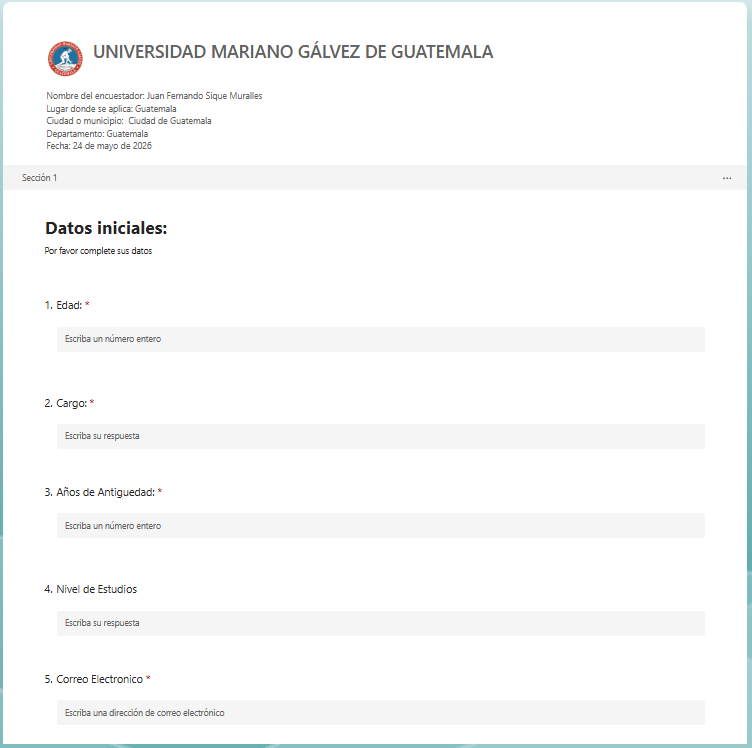
\includegraphics[width=\textwidth]{./imagenes/image8.png}
\end{figure}

\begin{figure}[H]
    \begin{flushleft}
        \textbf{Figura Anexo C2}\\
        \emph{Formato cuestionario en Blanco 2}
    \end{flushleft}
    \vspace{0.1cm}
    \centering
    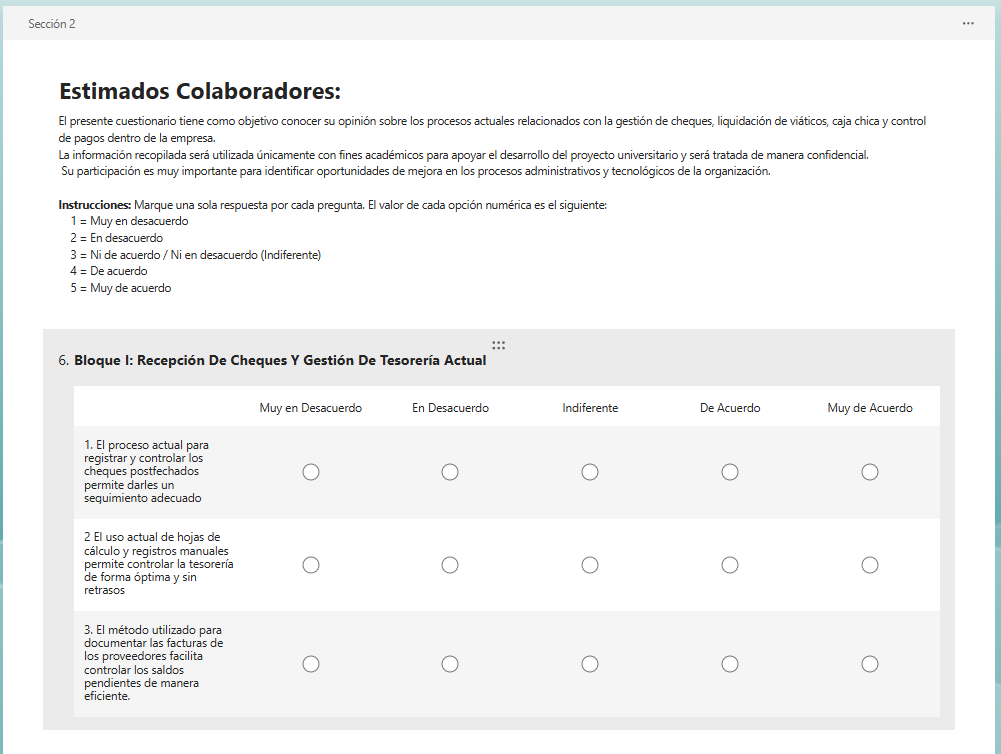
\includegraphics[width=\textwidth]{./imagenes/image9.png}
\end{figure}

\begin{figure}[H]
    \begin{flushleft}
        \textbf{Figura Anexo C3}\\
        \emph{Formato cuestionario en Blanco 3}
    \end{flushleft}
    \vspace{0.1cm}
    \centering
    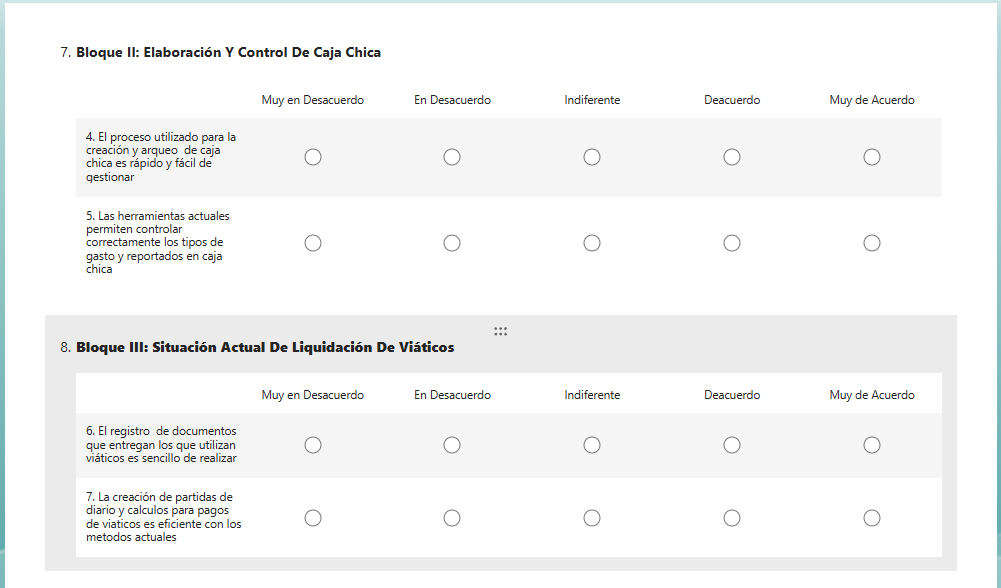
\includegraphics[width=\textwidth]{./imagenes/image10.png}
\end{figure}

\begin{figure}[H]
    \begin{flushleft}
        \textbf{Figura Anexo C4}\\
        \emph{Formato cuestionario en Blanco 4}
    \end{flushleft}
    \vspace{0.1cm}
    \centering
    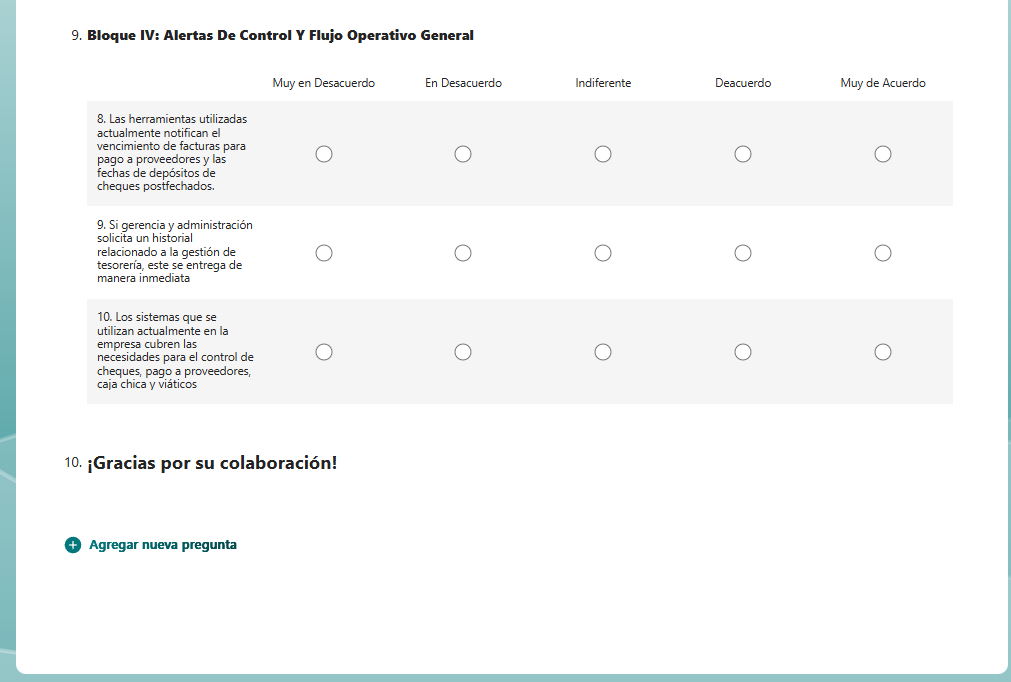
\includegraphics[width=\textwidth]{./imagenes/image11.png}
\end{figure}

\subsection{Muestra de Aplicación}\label{muestra-de-aplicacion}

\begin{figure}[H]
    \begin{flushleft}
        \textbf{Figura Anexo C5}\\
        \emph{Formato cuestionario 1 lleno 1}
    \end{flushleft}
    \vspace{0.1cm}
    \centering
    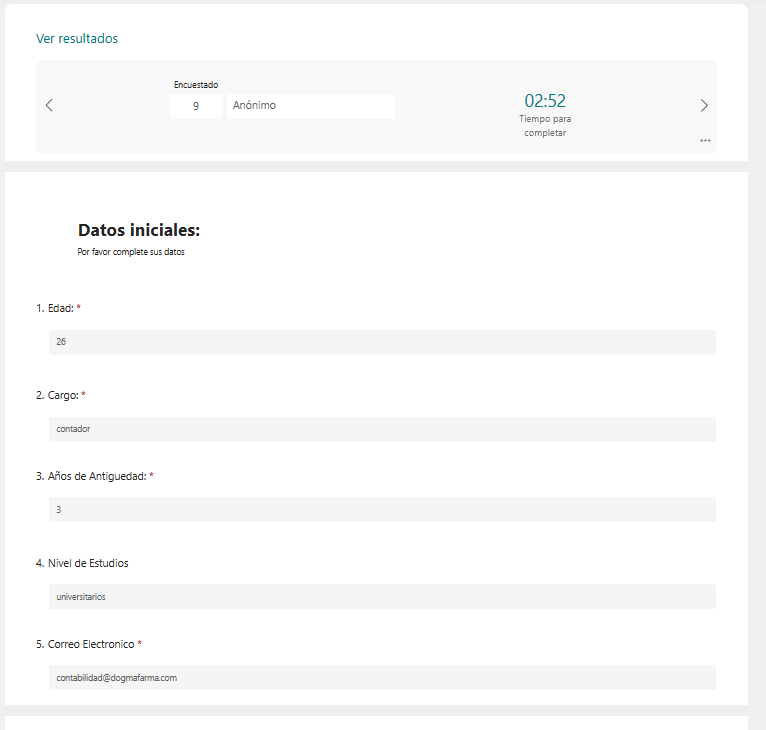
\includegraphics[width=\textwidth]{./imagenes/image12.png}
\end{figure}

\begin{figure}[H]
    \begin{flushleft}
        \textbf{Figura Anexo C6}\\
        \emph{Formato cuestionario 1 lleno 2}
    \end{flushleft}
    \vspace{0.1cm}
    \centering
    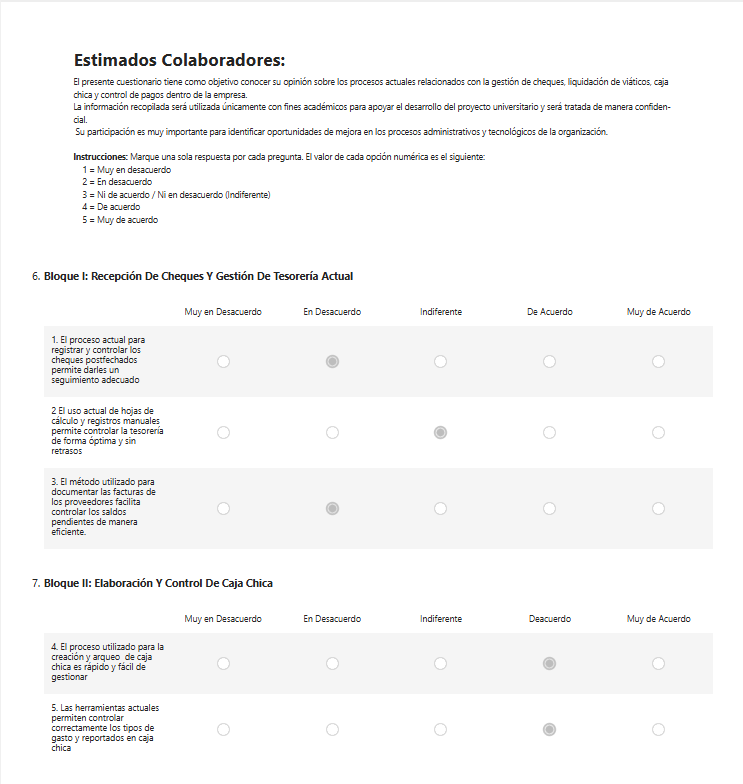
\includegraphics[width=\textwidth]{./imagenes/image13.png}
\end{figure}

\begin{figure}[H]
    \begin{flushleft}
        \textbf{Figura Anexo C7}\\
        \emph{Formato cuestionario 1 lleno 3}
    \end{flushleft}
    \vspace{0.1cm}
    \centering
    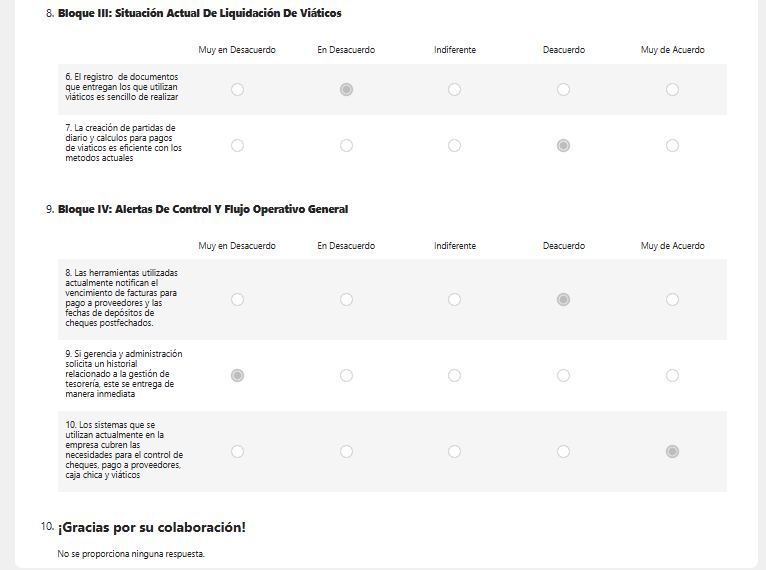
\includegraphics[width=\textwidth]{./imagenes/image14.png}
\end{figure}

\begin{figure}[H]
    \begin{flushleft}
        \textbf{Figura Anexo C8}\\
        \emph{Formato cuestionario 2 lleno 1}
    \end{flushleft}
    \vspace{0.1cm}
    \centering
    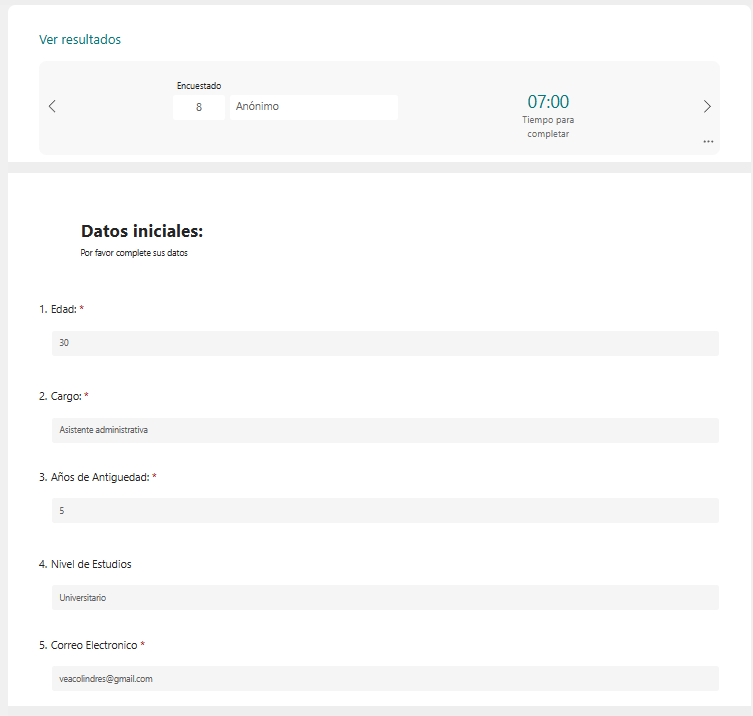
\includegraphics[width=\textwidth]{./imagenes/image15.png}
\end{figure}

\begin{figure}[H]
    \begin{flushleft}
        \textbf{Figura Anexo C9}\\
        \emph{Formato cuestionario 2 lleno 2}
    \end{flushleft}
    \vspace{0.1cm}
    \centering
    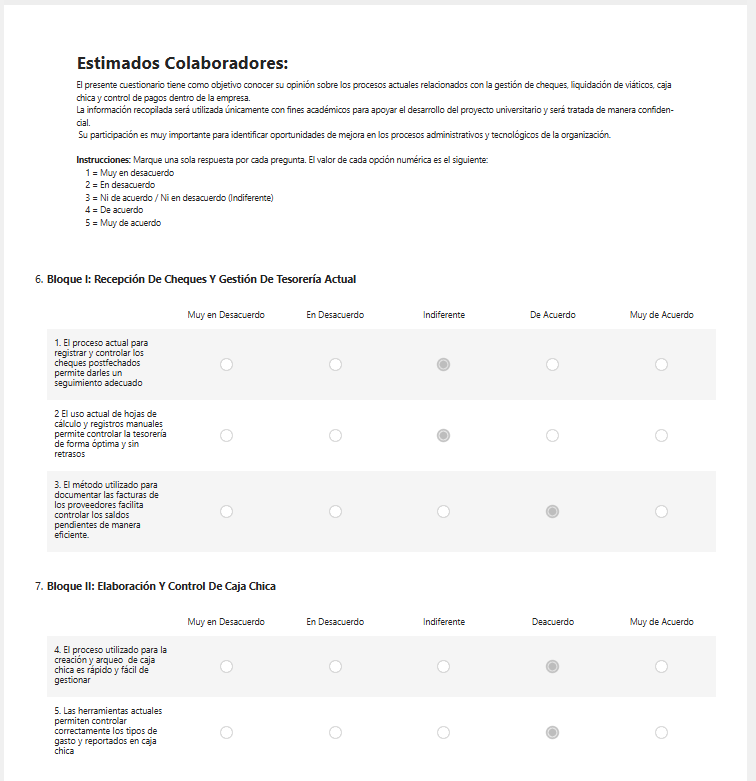
\includegraphics[width=\textwidth]{./imagenes/image16.png}
\end{figure}

\begin{figure}[H]
    \begin{flushleft}
        \textbf{Figura Anexo C10}\\
        \emph{Formato cuestionario 2 lleno 3}
    \end{flushleft}
    \vspace{0.1cm}
    \centering
    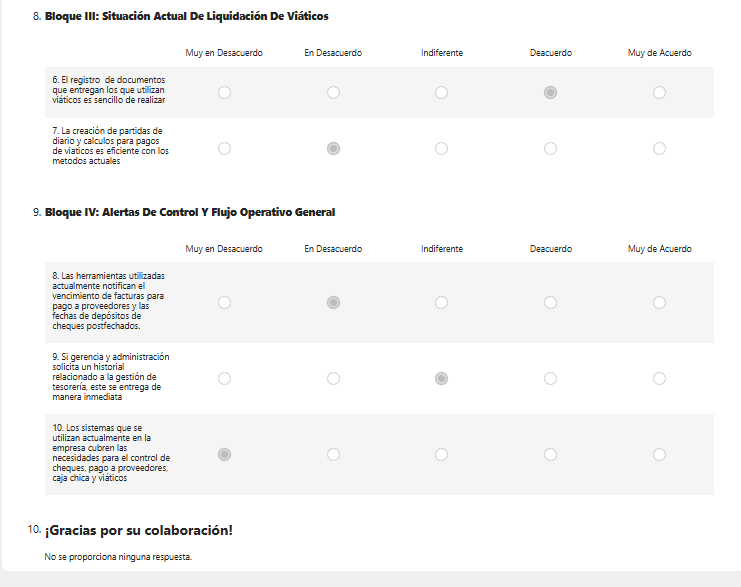
\includegraphics[width=\textwidth]{./imagenes/image17.png}
\end{figure}

\subsection{Interpretación de Escala de Likert}\label{interpretacion-de-escala-de-likert}

\begin{figure}[H]
    \begin{flushleft}
        \textbf{Figura Anexo C11}\\
        \emph{Resultado de la Escala de Likert}
    \end{flushleft}
    \vspace{0.1cm}
    \centering
    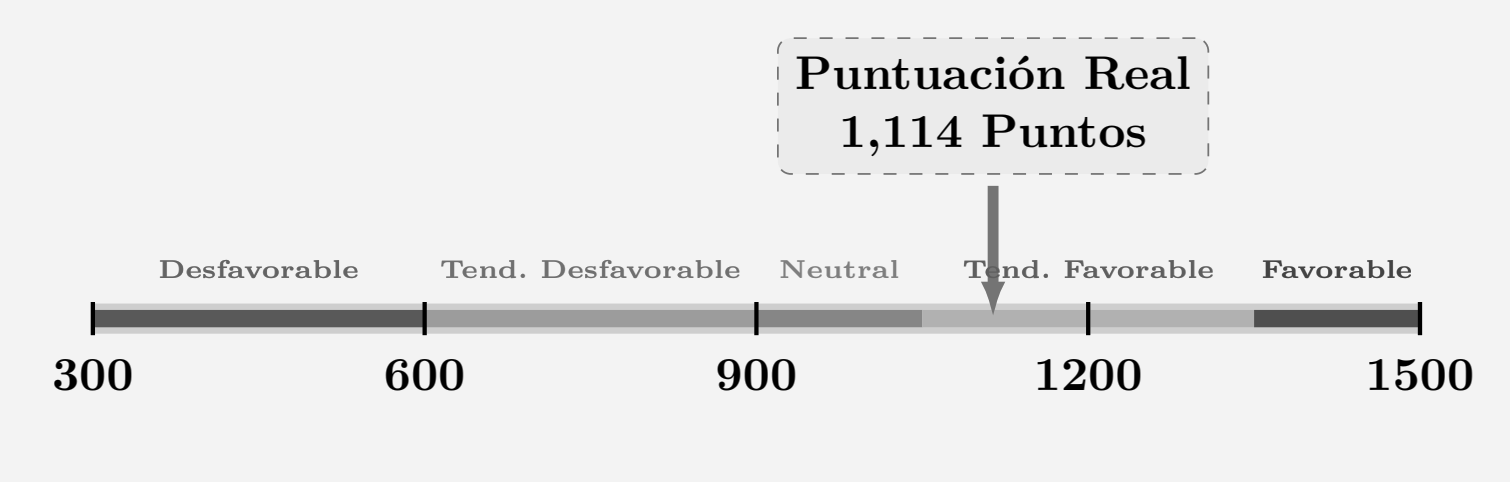
\includegraphics[width=\textwidth]{./imagenes/image18.png}
\end{figure}

\begin{figure}[H]
    \begin{flushleft}
        \textbf{Figura Anexo C12}\\
        \emph{Bloque I}
    \end{flushleft}
    \vspace{0.1cm}
    \centering
    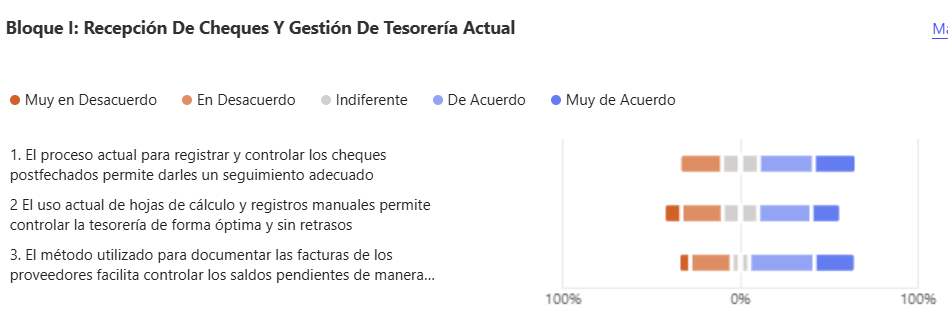
\includegraphics[width=\textwidth]{./imagenes/image19.png}
\end{figure}

\begin{table}[H]
\small
\begin{flushleft}
    \textbf{Tabla Anexo C1}\\[0.2cm]
    \emph{Bloque I (Porcentajes Tres preguntas)}
\end{flushleft}
\renewcommand{\arraystretch}{1.0}
\centering
\begin{tabular}{
    >{\raggedright\arraybackslash}p{2.6cm} 
    >{\raggedright\arraybackslash}p{1.6cm} 
    >{\raggedright\arraybackslash}p{1.6cm} 
    >{\raggedright\arraybackslash}p{1.6cm} 
    >{\raggedright\arraybackslash}p{2.0cm} 
    >{\raggedright\arraybackslash}p{2.3cm} 
    >{\raggedright\arraybackslash}p{1.8cm}
}
\toprule
\textbf{Preguntas} & \textbf{Muy de\newline Acuerdo} & \textbf{De\newline Acuerdo} & \textbf{Indiferente} & \textbf{En\newline Desacuerdo} & \textbf{Muy en\newline Desacuerdo} & \textbf{Sin\newline Respuesta} \\
\midrule
P.1 & 7 & 9 & 6 & 7 & 0 & 1 \\
P.2 & 5 & 9 & 6 & 7 & 3 & 0 \\
P.3 & 7 & 11 & 3 & 7 & 2 & 0 \\
\midrule
\textbf{Suma Bloque} & \textbf{19} & \textbf{29} & \textbf{15} & \textbf{21} & \textbf{5} & \textbf{1} \\
\textbf{Total (\%)} & \textbf{21.1\%} & \textbf{32.2\%} & \textbf{16.7\%} & \textbf{23.3\%} & \textbf{5.6\%} & \textbf{1.1\%} \\
\bottomrule
\end{tabular}
\end{table}

\begin{figure}[H]
    \begin{flushleft}
        \textbf{Figura Anexo C13}\\
        \emph{Bloque II}
    \end{flushleft}
    \vspace{0.1cm}
    \centering
    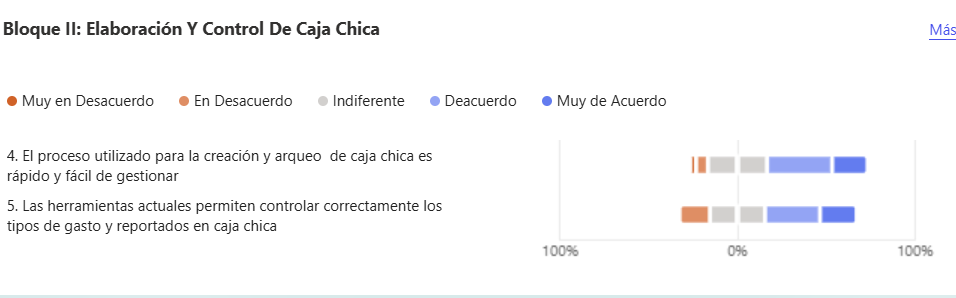
\includegraphics[width=\textwidth]{./imagenes/image20.png}
\end{figure}

\begin{table}[H]
\small
\begin{flushleft}
    \textbf{Tabla Anexo C2}\\[0.2cm]
    \emph{Bloque II (Porcentajes dos preguntas)}
\end{flushleft}
\renewcommand{\arraystretch}{1.0}
\centering
\begin{tabular}{
    >{\raggedright\arraybackslash}p{2.6cm} 
    >{\raggedright\arraybackslash}p{1.6cm} 
    >{\raggedright\arraybackslash}p{1.6cm} 
    >{\raggedright\arraybackslash}p{1.6cm} 
    >{\raggedright\arraybackslash}p{2.0cm} 
    >{\raggedright\arraybackslash}p{2.3cm} 
    >{\raggedright\arraybackslash}p{1.8cm}
}
\toprule
\textbf{Preguntas} & \textbf{Muy de\newline Acuerdo} & \textbf{De\newline Acuerdo} & \textbf{Indiferente} & \textbf{En\newline Desacuerdo} & \textbf{Muy en\newline Desacuerdo} & \textbf{Sin\newline Respuesta} \\
\midrule
P.4 & 6 & 11 & 10 & 2 & 1 & 0 \\
P.5 & 6 & 9 & 9 & 5 & 0 & 1 \\
\midrule
\textbf{Suma Bloque} & \textbf{12} & \textbf{20} & \textbf{19} & \textbf{7} & \textbf{1} & \textbf{1} \\
\textbf{Total (\%)} & \textbf{20.0\%} & \textbf{33.3\%} & \textbf{31.7\%} & \textbf{11.7\%} & \textbf{1.7\%} & \textbf{1.6\%} \\
\bottomrule
\end{tabular}
\end{table}

\begin{figure}[H]
    \begin{flushleft}
        \textbf{Figura Anexo C14}\\
        \emph{Bloque III}
    \end{flushleft}
    \vspace{0.1cm}
    \centering
    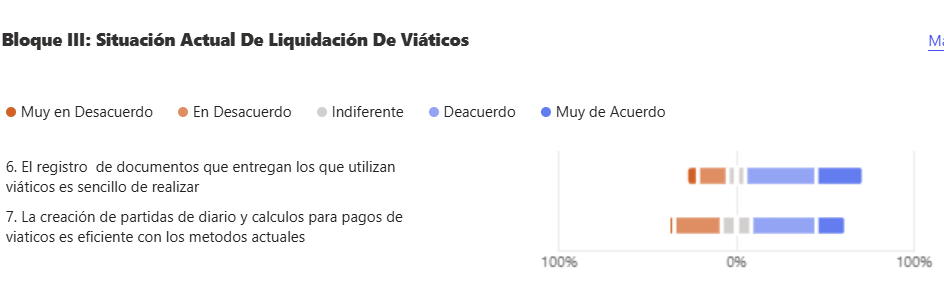
\includegraphics[width=\textwidth]{./imagenes/image21.png}
\end{figure}

\begin{table}[H]
\small
\begin{flushleft}
    \textbf{Tabla Anexo C3}\\[0.2cm]
    \emph{Bloque III (Porcentajes Dos preguntas)}
\end{flushleft}
\renewcommand{\arraystretch}{1.0}
\centering
\begin{tabular}{
    >{\raggedright\arraybackslash}p{2.6cm} 
    >{\raggedright\arraybackslash}p{1.6cm} 
    >{\raggedright\arraybackslash}p{1.6cm} 
    >{\raggedright\arraybackslash}p{1.6cm} 
    >{\raggedright\arraybackslash}p{2.0cm} 
    >{\raggedright\arraybackslash}p{2.3cm} 
    >{\raggedright\arraybackslash}p{1.8cm}
}
\toprule
\textbf{Preguntas} & \textbf{Muy de\newline Acuerdo} & \textbf{De\newline Acuerdo} & \textbf{Indiferente} & \textbf{En\newline Desacuerdo} & \textbf{Muy en\newline Desacuerdo} & \textbf{Sin\newline Respuesta} \\
\midrule
P.6 & 8 & 12 & 3 & 5 & 2 & 0 \\
P.7 & 5 & 11 & 5 & 8 & 1 & 0 \\
\midrule
\textbf{Suma Bloque} & \textbf{13} & \textbf{23} & \textbf{8} & \textbf{13} & \textbf{3} & \textbf{0} \\
\textbf{Total (\%)} & \textbf{21.7\%} & \textbf{38.3\%} & \textbf{13.3\%} & \textbf{21.7\%} & \textbf{5.0\%} & \textbf{0.0\%} \\
\bottomrule
\end{tabular}
\end{table}

\begin{figure}[H]
\begin{flushleft}
    \textbf{Figura Anexo C15}\\
    \emph{Bloque IV}
\end{flushleft}
\vspace{0.1cm}
\centering
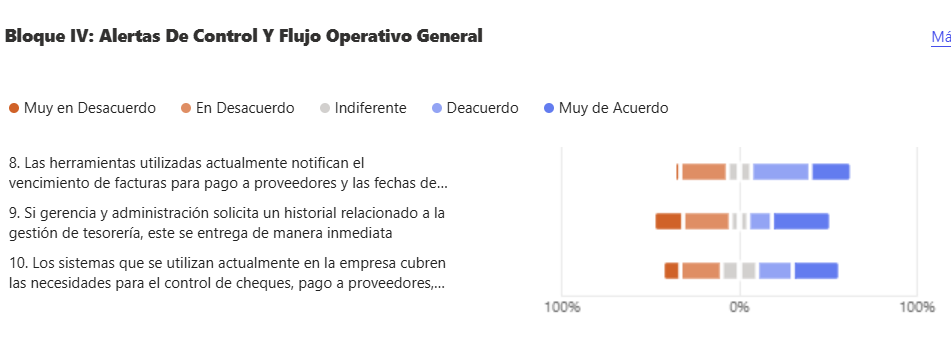
\includegraphics[width=\textwidth]{./imagenes/image22.png}
\end{figure}

\begin{table}[H]
\small
\begin{flushleft}
    \textbf{Tabla Anexo C4}\\[0.2cm]
    \emph{Bloque IV (Porcentajes Tres preguntas)}
\end{flushleft}
\renewcommand{\arraystretch}{1.0}
\centering
\begin{tabular}{
    >{\raggedright\arraybackslash}p{2.6cm} 
    >{\raggedright\arraybackslash}p{1.6cm} 
    >{\raggedright\arraybackslash}p{1.6cm} 
    >{\raggedright\arraybackslash}p{1.6cm} 
    >{\raggedright\arraybackslash}p{2.0cm} 
    >{\raggedright\arraybackslash}p{2.3cm} 
    >{\raggedright\arraybackslash}p{1.8cm}
}
\toprule
\textbf{Preguntas} & \textbf{Muy de\newline Acuerdo} & \textbf{De\newline Acuerdo} & \textbf{Indiferente} & \textbf{En\newline Desacuerdo} & \textbf{Muy en\newline Desacuerdo} & \textbf{Sin\newline Respuesta} \\
\midrule
P.8 & 7 & 10 & 4 & 8 & 1 & 0 \\
P.9 & 10 & 4 & 3 & 8 & 5 & 0 \\
P.10 & 8 & 6 & 6 & 7 & 3 & 0 \\
\midrule
\textbf{Suma Bloque} & \textbf{25} & \textbf{20} & \textbf{13} & \textbf{23} & \textbf{9} & \textbf{0} \\
\textbf{Total (\%)} & \textbf{27.8\%} & \textbf{22.2\%} & \textbf{14.4\%} & \textbf{25.6\%} & \textbf{10.0\%} & \textbf{0.0\%} \\
\bottomrule
\end{tabular}
\end{table}

% =========================================================
% APÉNDICES (Numeración de página continua en Arábigos)
% =========================================================

\appendix
\renewcommand{\thesection}{\Alph{section}}
\counterwithin{figure}{section}
\counterwithin{table}{section}
\renewcommand{\thefigure}{\thesection\arabic{figure}}
\renewcommand{\thetable}{\thesection\arabic{table}}

% Entrada principal en el Índice General
\addcontentsline{toc}{section}{Apéndice}

% Manual de Usuario del Sistema Web de gestión contable.
% Este archivo se incorpora directamente desde main.tex como Apéndice A.
% Las capturas anotadas utilizan numeración correlativa y pasos operativos.

\newpage
\section*{Apéndice}\label{Apendice}
\addcontentsline{toc}{section}{Apéndice}

\appendix
% El Manual de Usuario corresponde al Apéndice A.
\setcounter{section}{1}
\renewcommand{\thesection}{\Alph{section}}
\renewcommand{\thesubsection}{\thesection.\arabic{subsection}}
\renewcommand{\thefigure}{\thesection\arabic{figure}}
\renewcommand{\thetable}{\thesection\arabic{table}}
\setcounter{figure}{0}
\setcounter{table}{0}
\setcounter{tocdepth}{0}
\captionsetup{list=false}
\pagestyle{cuerpo}

\setcounter{subsection}{0}
\subsection{Manual de Usuario}\label{ap:Manual-de-Usuario}
\phantomsection
\addcontentsline{toc}{section}{Apéndice A Manual de Usuario}
\begin{center}
\vspace*{2cm}
{\Large\textbf{APÉNDICE A}}\par
\vspace{1.5cm}
{\Large\textbf{MANUAL DE USUARIO}}\par
\vspace{0.8cm}
{\large Sistema Web de gestión contable}\par
\vspace{2cm}
\begin{minipage}{0.82\textwidth}
\centering
Guía para el ingreso al sistema, consulta y registro de facturas FEL/SAT, cheques posfechados, caja chica, viáticos, proveedores, calendario, nomenclatura contable y reportes.
\end{minipage}
\vfill
Documento complementario del trabajo de graduación\par
\end{center}


\setlength{\parindent}{1.27cm}
\setlength{\parskip}{0pt}
\setstretch{2.0}

\subsubsection{Introducción}
Este manual orienta al usuario final en el uso del Sistema Web para el control de facturas FEL/SAT, cheques posfechados, caja chica, viáticos, proveedores, nomenclatura contable, calendario y reportes. Cada pantalla se presenta con una captura del prototipo funcional y una versión anotada. Los números rojos de la imagen corresponden directamente a los pasos descritos debajo de ella.

Los datos que aparecen en las figuras son demostrativos. El usuario debe aplicar, además, las políticas internas de autorización, revisión y resguardo de documentos contables.

\subsubsection{Requisitos del sistema}
El correcto funcionamiento y uso del Sistema Web depende de que el equipo del usuario tenga acceso a la red institucional, un navegador actualizado y las credenciales autorizadas. Los requisitos se organizan entre el lado del cliente, utilizado por el personal operativo, y el lado del servidor, administrado por el personal técnico.

\paragraph{Requisitos del lado del cliente}
El lado del cliente corresponde al equipo desde el cual el usuario consulta y registra información. El sistema debe ejecutarse en un navegador compatible con aplicaciones web modernas y con acceso habilitado a la dirección institucional de la plataforma.

\paragraph{Infraestructura de software del cliente}
\begin{itemize}
\item Navegador web actualizado, como Google Chrome, Mozilla Firefox, Microsoft Edge o Safari.
\item JavaScript habilitado para permitir la ejecución de la interfaz desarrollada en Angular.
\item Cookies y almacenamiento local habilitados cuando sean necesarios para conservar la sesión autorizada.
\item Sistema operativo de escritorio compatible con el navegador instalado.
\item Cuenta de usuario activa, con el perfil y los permisos asignados por la organización.
\end{itemize}

\paragraph{Conectividad del cliente}
El equipo debe mantener una conexión estable con la red institucional o con el servicio autorizado para acceder al sistema. Si la conexión se interrumpe durante un registro, el usuario debe verificar si la operación fue guardada antes de repetirla, con el fin de evitar duplicidad de documentos o movimientos.

\paragraph{Requisitos del lado del servidor}
El lado del servidor debe mantener disponibles los servicios del frontend Angular, el backend desarrollado en Python/FastAPI y la base de datos PostgreSQL. La configuración debe separar las credenciales y variables de los ambientes de desarrollo, pruebas y producción.

\paragraph{Entorno de software del servidor}
\begin{itemize}
\item Sistema operativo de servidor compatible con Python, Angular y PostgreSQL.
\item Runtime de Python y dependencias del backend documentados en el archivo de configuración del proyecto.
\item Servicio backend Python/FastAPI para autenticación, validación y reglas de negocio.
\item Servicio de publicación del frontend Angular con conexión segura al backend.
\item PostgreSQL para almacenar usuarios, facturas, cheques, movimientos, cuentas, proveedores y reportes.
\item Certificado SSL/TLS y configuración de acceso restringido para proteger la comunicación.
\end{itemize}

\paragraph{Dimensionamiento de referencia}
La siguiente tabla presenta una referencia mínima para el ambiente del servidor. El dimensionamiento definitivo debe revisarse según el número de usuarios, el volumen de facturas y las políticas de infraestructura de la organización.

\begin{longtable}{p{4.0cm}p{4.3cm}p{4.3cm}}
\caption{Requisitos de infraestructura de referencia}\label{tab:A_requisitos_sistema}\\
\toprule
\textbf{Componente} & \textbf{Configuración mínima} & \textbf{Configuración recomendada}\\
\midrule
Procesador & 1 núcleo virtual de 64 bits & 2 núcleos virtuales o físicos dedicados\\
Memoria RAM & 2 GB disponibles & 4 GB o superior\\
Almacenamiento & 10 GB libres para aplicación, logs y configuración & 30 GB libres en unidad de estado sólido\\
Base de datos & PostgreSQL configurado con respaldo periódico & PostgreSQL con almacenamiento separado y monitoreo\\
Red & Conexión estable para atender las solicitudes del sistema & Enlace institucional con monitoreo de disponibilidad\\
Respaldo & Copia periódica de la base de datos & Copia automática externa y prueba de restauración\\
\bottomrule
\end{longtable}

\textit{Nota.} Los valores son de referencia para la instalación y deben ajustarse al crecimiento de usuarios, documentos y registros contables.

\subsubsection{Acceso al sistema}
Abra el navegador, escriba la dirección web proporcionada por el administrador y espere a que se muestre la pantalla de acceso.

\subsubsection{Ingreso al sistema}
En la sección de acceso, siga los pasos ilustrados en la captura anotada para ingresar al sistema.

\subsubsection{Descripción general del sistema}
El Sistema Web organiza en un menú lateral los módulos de Facturas FEL/SAT, Cheques, Caja chica, Viáticos, Proveedores, Calendario, Nomenclatura y Reportes. El Panel principal presenta alertas e indicadores del período activo, mientras que cada módulo permite registrar, consultar y dar seguimiento a las operaciones autorizadas.

\begin{figure}[H]
    \centering
    \caption{Pantalla de acceso con anotaciones numeradas.}
    \label{fig:manual_usuario_pantalla_01_login_anotada}
    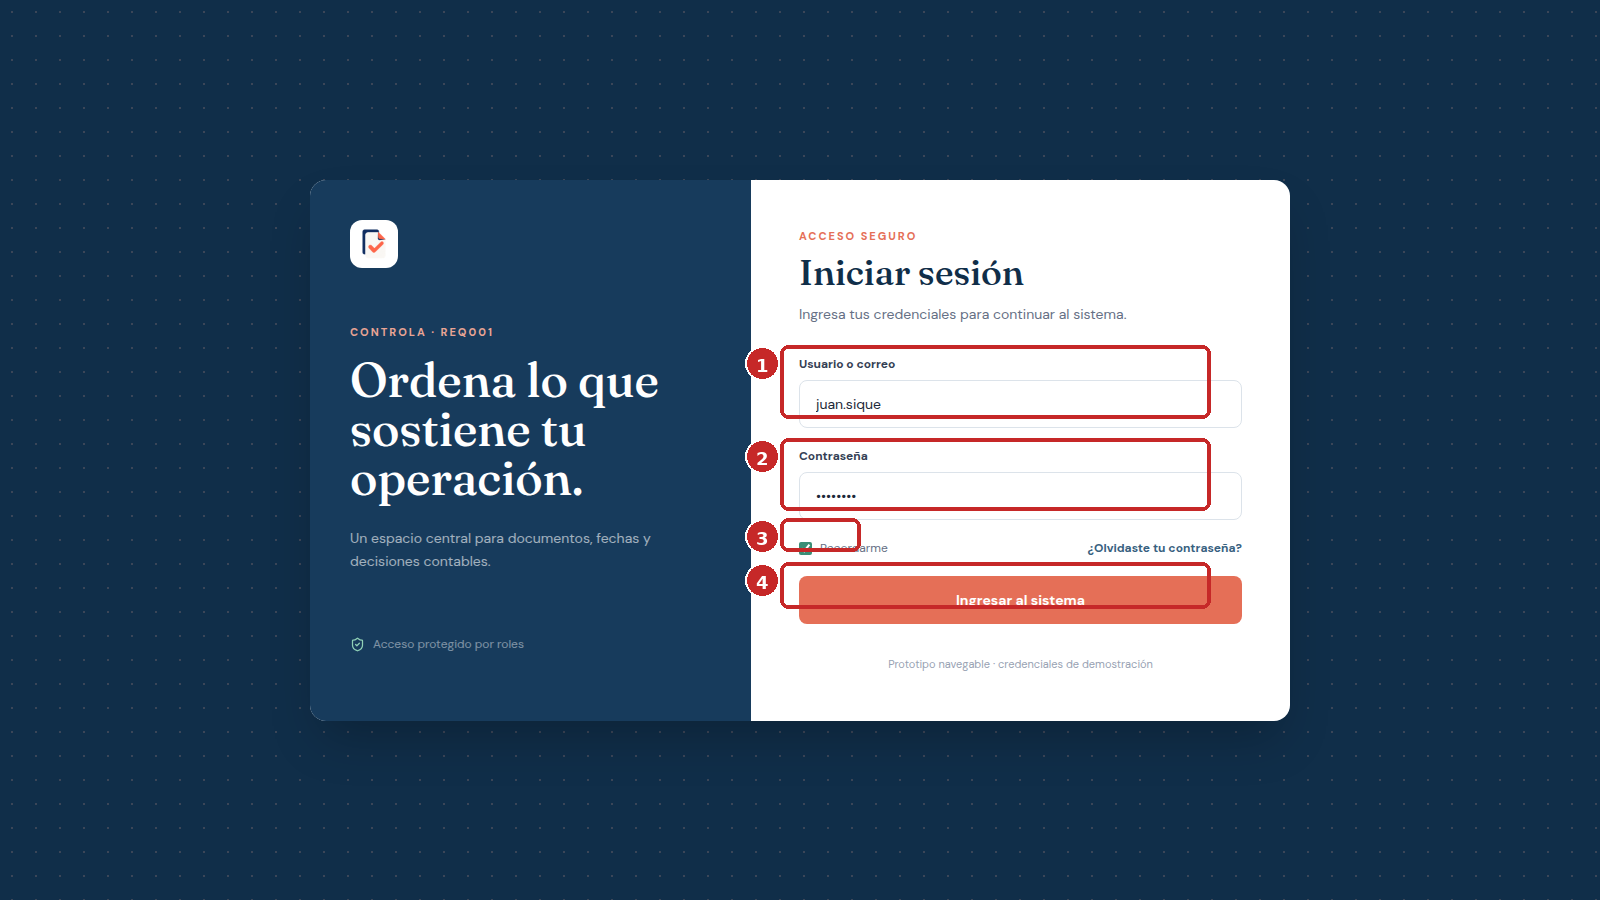
\includegraphics[width=0.92\linewidth]{capturas_reales/anotadas/pantalla_01_login_anotada.png}
    \caption*{Nota. Elaboración propia a partir del prototipo funcional.}
\end{figure}

\begin{enumerate}
\item Haga clic en el campo de usuario y escriba el nombre de usuario o correo electrónico habilitado.
\item Haga clic en el campo de contraseña y escriba la clave sin agregar espacios al inicio o al final.
\item Haga clic en la casilla ``Recordarme'' únicamente si el equipo es institucional y cumple las políticas de seguridad.
\item Haga clic en ``Ingresar al sistema''.
\item El sistema validará las credenciales y mostrará el Panel principal. Si aparece un mensaje de error, revise los datos y solicite apoyo al administrador cuando sea necesario.
\end{enumerate}

\subsubsection{Uso del sistema}
Las instrucciones siguientes describen las operaciones principales del sistema mediante capturas anotadas. Realice cada paso en el orden indicado y verifique el mensaje mostrado antes de continuar.

\subsubsection{Panel principal}
El Panel principal concentra la información operativa del período contable seleccionado.

\begin{figure}[H]
    \centering
    \caption{Panel principal con anotaciones numeradas.}
    \label{fig:manual_usuario_pantalla_02_dashboard_anotada}
    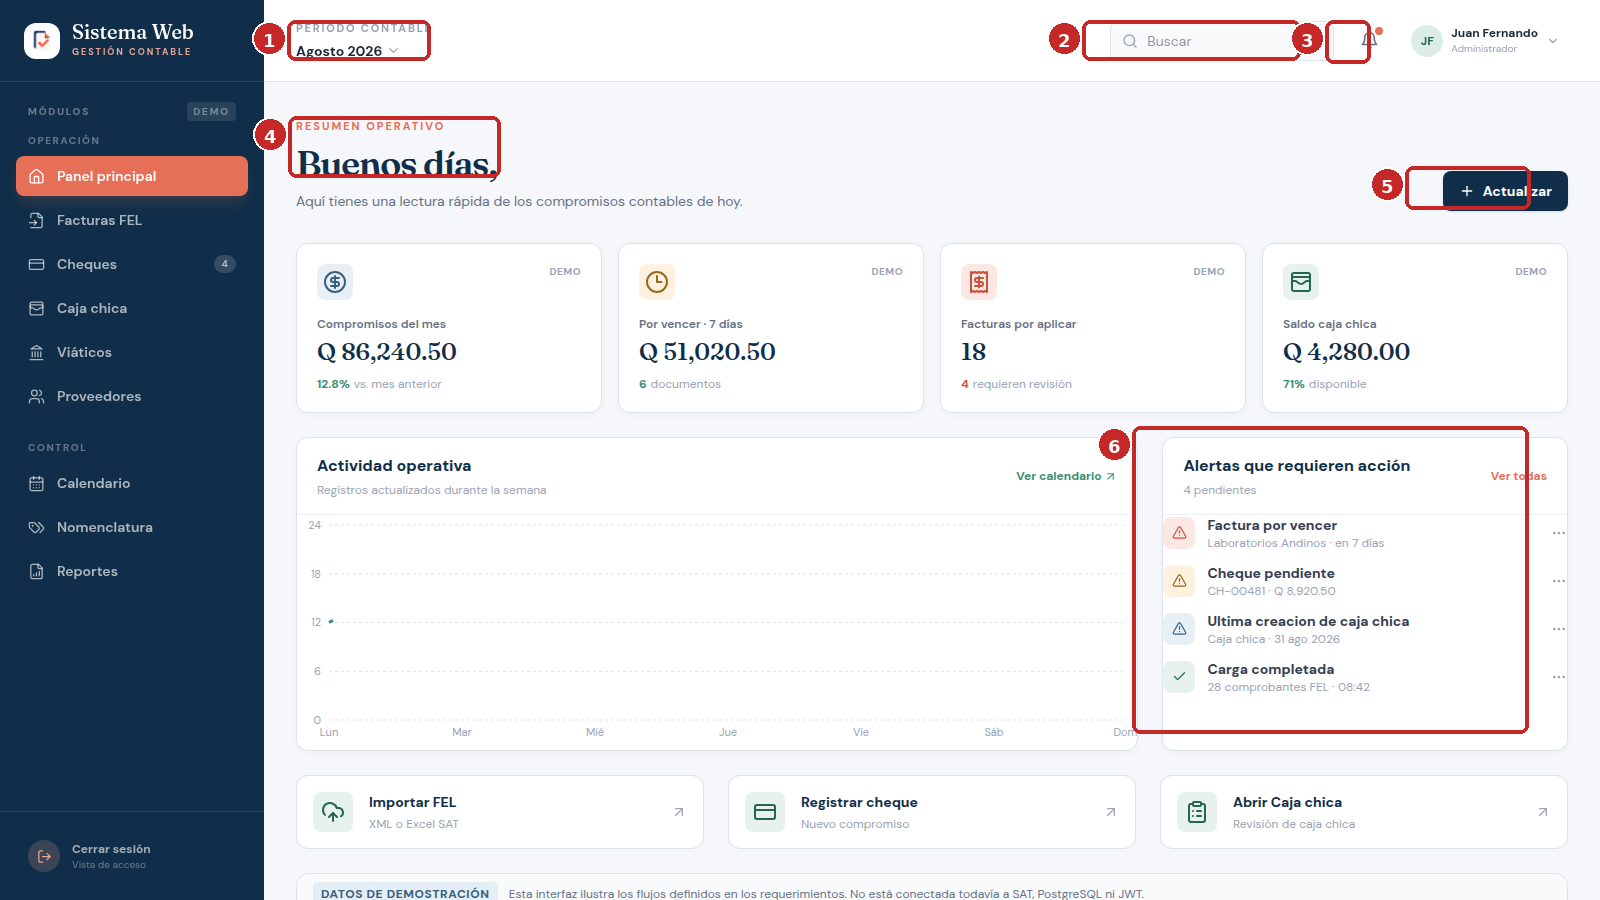
\includegraphics[width=0.92\linewidth]{capturas_reales/anotadas/pantalla_02_dashboard_anotada.png}
    \caption*{Nota. Elaboración propia a partir del prototipo funcional.}
\end{figure}

\begin{enumerate}
\item Revise el período contable activo.
\item Haga clic en ``Buscar'' y escriba el criterio de consulta.
\item Revise las alertas operativas pendientes.
\item Revise los indicadores de compromisos, vencimientos, facturas y saldo de Caja chica.
\item Haga clic en ``Actualizar'' para refrescar la información mostrada.
\item Revise las alertas y seleccione la que requiera atención.
\item Para cambiar de módulo, seleccione una opción del menú lateral, por ejemplo ``Facturas FEL'', ``Cheques'', ``Caja chica'', ``Viáticos'', ``Proveedores'', ``Calendario'', ``Nomenclatura'' o ``Reportes''.
\end{enumerate}

\subsubsection{Facturas FEL/SAT}
Este módulo permite importar archivos XML o Excel descargados del portal SAT, revisar comprobantes y detectar duplicados o documentos que requieren revisión.

\begin{figure}[H]
    \centering
    \caption{Módulo de Facturas FEL/SAT con anotaciones numeradas.}
    \label{fig:manual_usuario_pantalla_03_facturas_fel_anotada}
    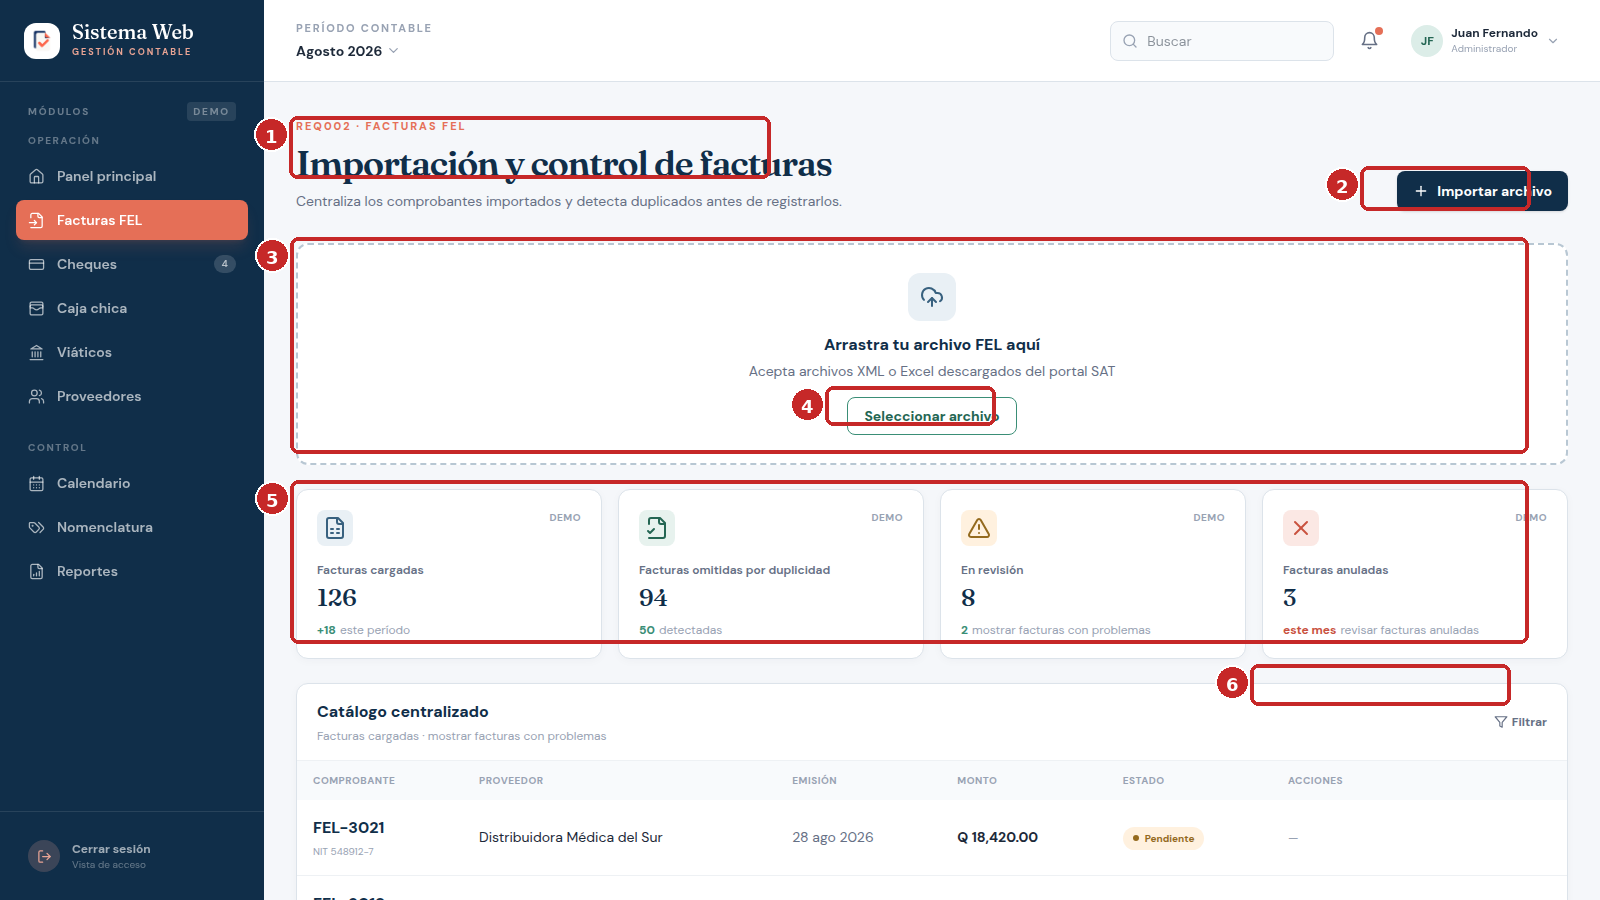
\includegraphics[width=0.92\linewidth]{capturas_reales/anotadas/pantalla_03_facturas_fel_anotada.png}
    \caption*{Nota. Elaboración propia a partir del prototipo funcional.}
\end{figure}

\begin{enumerate}
\item confirme que se encuentra en ``Facturas FEL''.
\item presione ``Importar archivo'' para iniciar la carga.
\item arrastre el archivo FEL al área indicada o presione ``Seleccionar archivo''.
\item espere a que el sistema lea el XML o Excel y actualice los indicadores.
\item consulte el catálogo centralizado y revise comprobante, proveedor, fecha, monto y estado.
\item utilice ``Editar'', ``Aprobar'' o ``Eliminar'' cuando esas acciones estén habilitadas para el registro.
\item Si una factura no puede clasificarse automáticamente, diríjase a la asignación correspondiente y seleccione manualmente una cuenta de Nomenclatura.
\end{enumerate}

\subsubsection{Cheques posfechados}
El módulo registra los cheques, sus bancos, fechas, clientes, estados y la información relacionada con la factura.

\begin{figure}[H]
    \centering
    \caption{Módulo de Cheques con anotaciones numeradas.}
    \label{fig:manual_usuario_pantalla_04_cheques_anotada}
    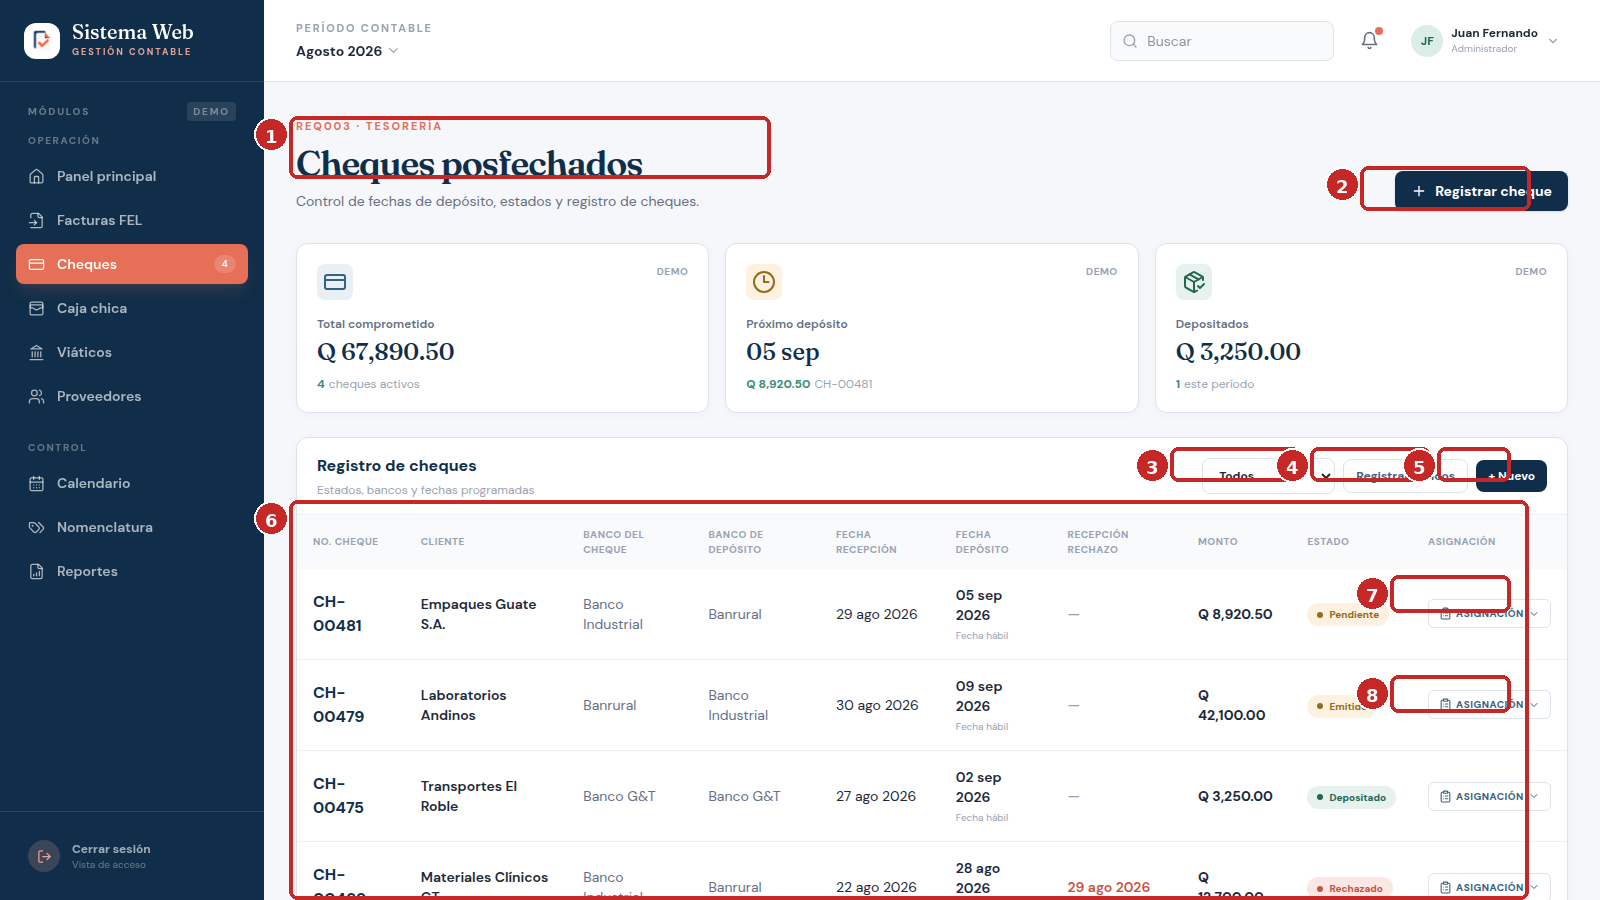
\includegraphics[width=0.92\linewidth]{capturas_reales/anotadas/pantalla_04_cheques_anotada.png}
    \caption*{Nota. Elaboración propia a partir del prototipo funcional.}
\end{figure}

\begin{enumerate}
\item Revise el resumen de compromisos, próximo depósito y cheques depositados.
\item Filtre la tabla por estado mediante la lista desplegable.
\item Haga clic en ``Registrar bancos'' para mantener los bancos disponibles.
\item Haga clic en ``Nuevo'' para registrar un cheque.
\item Revise la tabla con número de cheque, cliente, banco del cheque, banco de depósito, fecha de recepción, fecha de depósito, recepción de rechazo, monto y estado.
\item Haga clic en ``Asignación'' en el cheque que desea consultar.
\item Revise la fecha de factura, número de factura, visitador, número de recibo y días vencidos.
\item Repita la consulta para otro cheque cuando necesite comparar sus datos antes de registrar o dar seguimiento.
\end{enumerate}

\subsubsection{Caja chica}
Caja chica permite llamar una factura FEL por número, registrar recibos u otros documentos, asignar la cuenta contable y preparar la partida.

\begin{figure}[H]
    \centering
    \caption{Módulo de Caja chica con anotaciones numeradas.}
    \label{fig:manual_usuario_pantalla_05_caja_chica_anotada}
    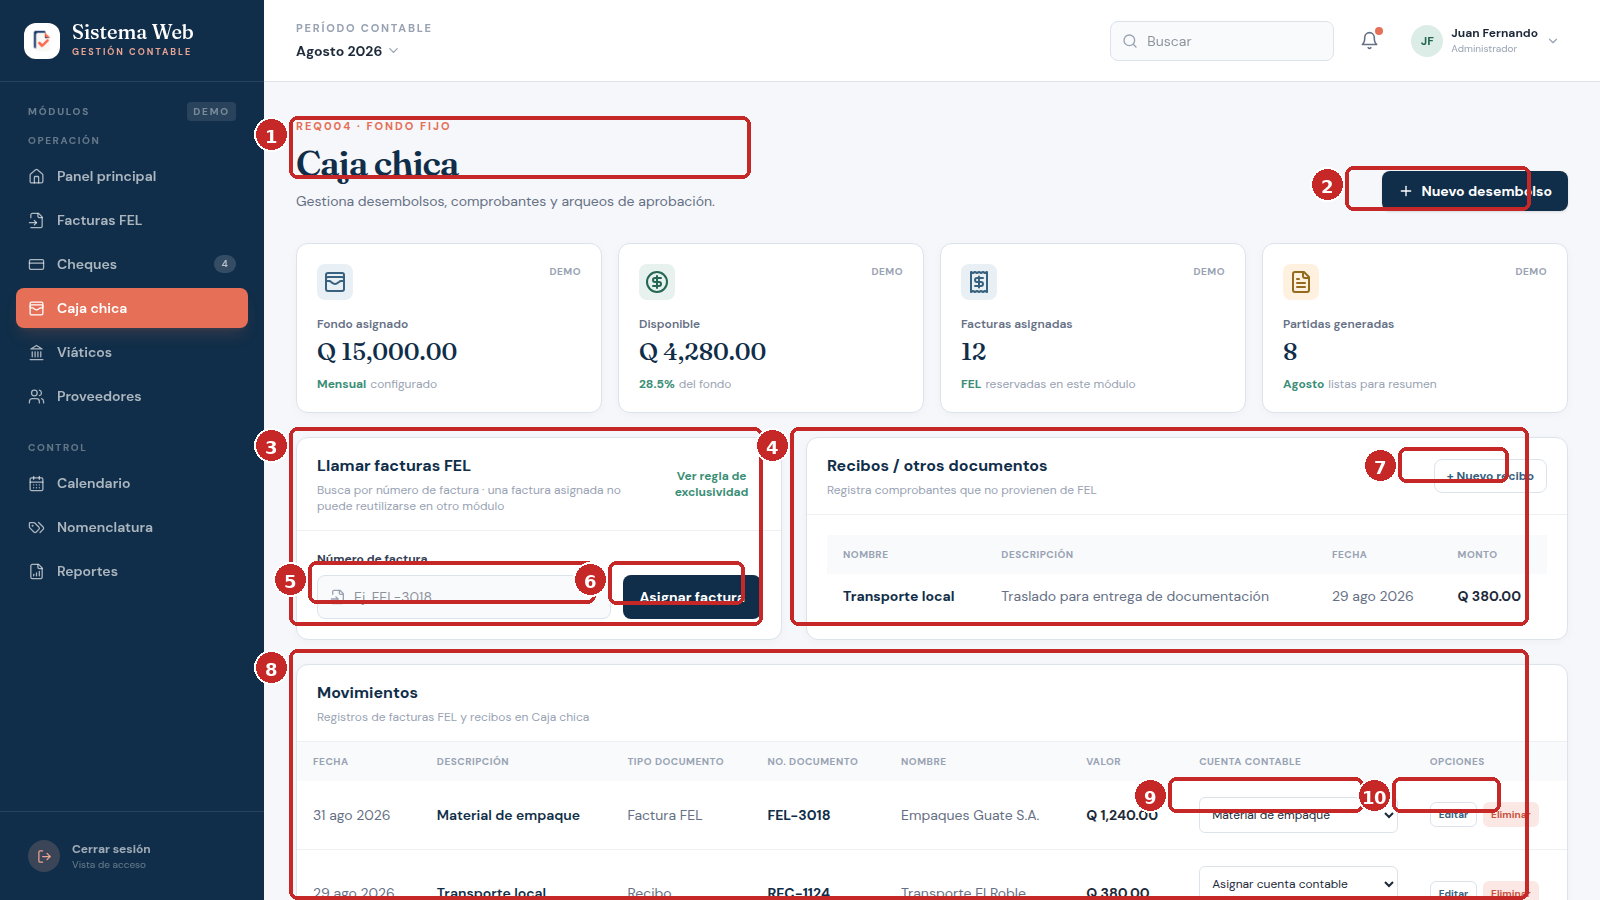
\includegraphics[width=0.92\linewidth]{capturas_reales/anotadas/pantalla_05_caja_chica_anotada.png}
    \caption*{Nota. Elaboración propia a partir del prototipo funcional.}
\end{figure}

\begin{enumerate}
\item revise el fondo asignado, disponible, facturas asignadas y partidas generadas.
\item escriba el número de factura FEL y presione ``Asignar factura''.
\item presione ``Nuevo recibo'' para registrar un documento que no proviene de FEL.
\item complete la fecha, descripción, tipo de documento, número, nombre y valor del movimiento.
\item revise la cuenta contable sugerida para el movimiento.
\item cuando la cuenta no sea reconocida, seleccione manualmente una cuenta registrada en Nomenclatura.
\item use ``Editar'' para corregir la descripción o los datos del movimiento y ``Eliminar'' solamente con autorización.
\item revise la tabla de Movimientos antes de generar la partida.
\item verifique los importes del Debe y las cuentas de gasto e IVA.
\item revise la contrapartida en el Haber y presione ``Imprimir resumen'' para preparar el documento.
\end{enumerate}

\subsubsection{Viáticos}
Viáticos administra colaboradores, territorios, giras, categorías de gasto y partidas automáticas.

\begin{figure}[H]
    \centering
    \caption{Módulo de Viáticos con anotaciones numeradas.}
    \label{fig:manual_usuario_pantalla_06_viaticos_anotada}
    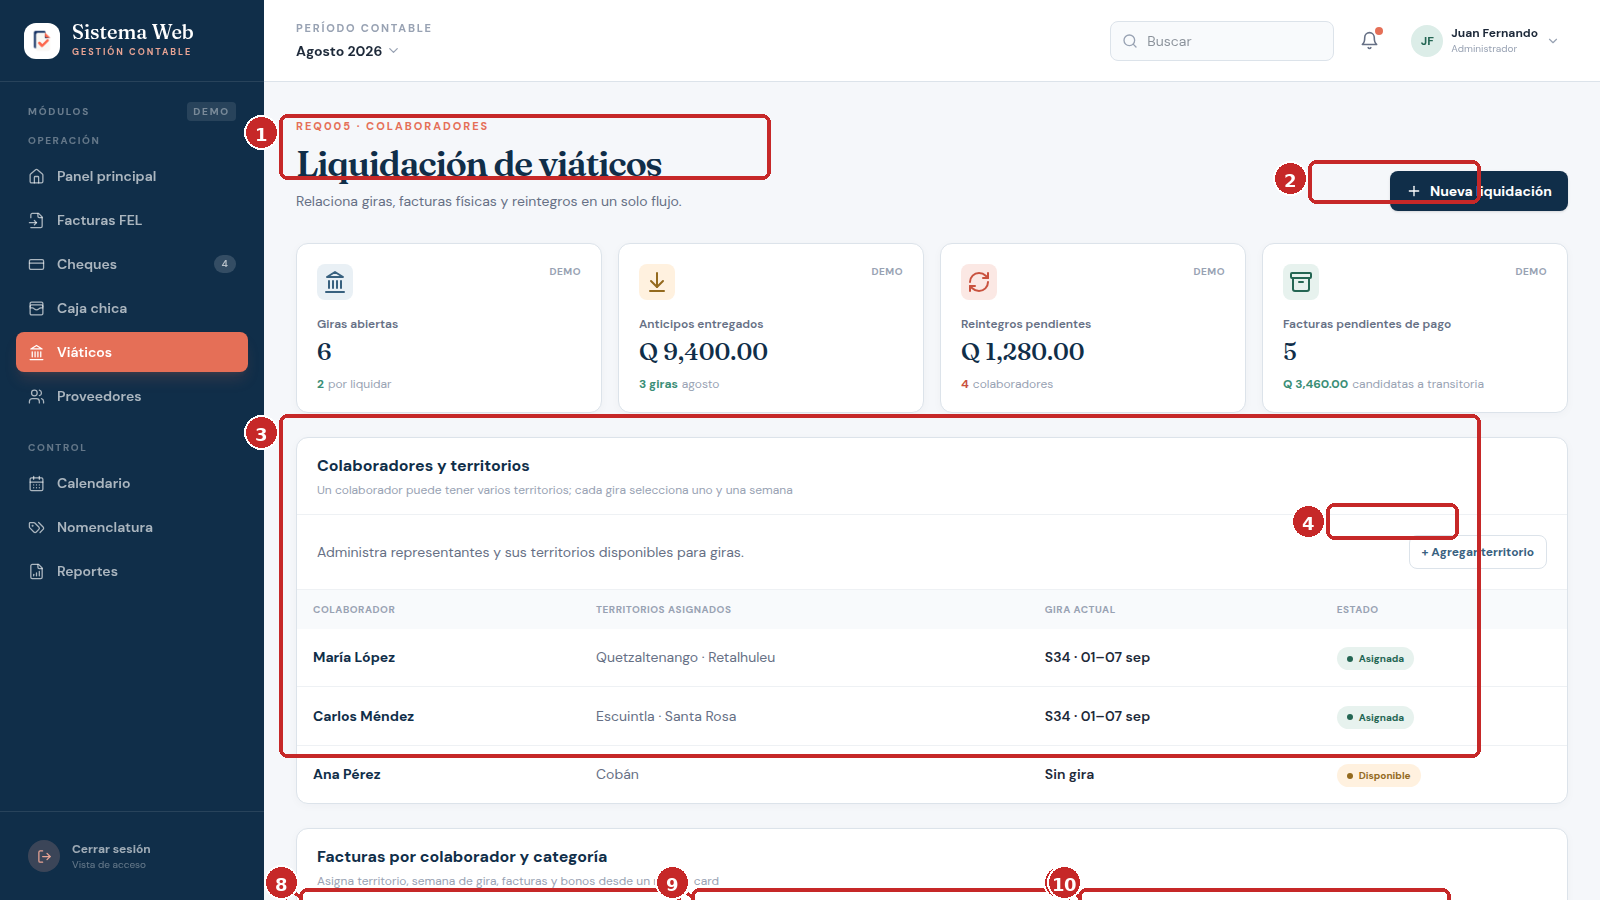
\includegraphics[width=0.92\linewidth]{capturas_reales/anotadas/pantalla_06_viaticos_anotada.png}
    \caption*{Nota. Elaboración propia a partir del prototipo funcional.}
\end{figure}

\begin{enumerate}
\item Revise las giras abiertas, anticipos, reintegros y facturas pendientes de pago.
\item Haga clic en ``Agregar territorio'' cuando deba asociar un territorio a un colaborador.
\item Seleccione el colaborador, el territorio y la semana de gira.
\item Seleccione la categoría ``Viáticos'', ``Movilidad'' o ``Actividades'' y haga clic en ``Asignar facturas''.
\item Recuerde que Movilidad está disponible durante la primera semana del mes según la regla del sistema.
\item Registre bonos u otros gastos indicando nombre, descripción y monto.
\item Revise la partida semanal y haga clic en ``Generar partida semanal''.
\item Haga clic en ``Generar cuenta transitoria'' para agrupar facturas pendientes de pago.
\end{enumerate}

\subsubsection{Asignación de facturas}
Esta pantalla permite vincular una factura con un colaborador, una gira, una categoría y una cuenta contable.

\begin{figure}[H]
    \centering
    \caption{Pantalla de asignación de facturas con anotaciones numeradas.}
    \label{fig:manual_usuario_pantalla_07_asignacion_facturas_anotada}
    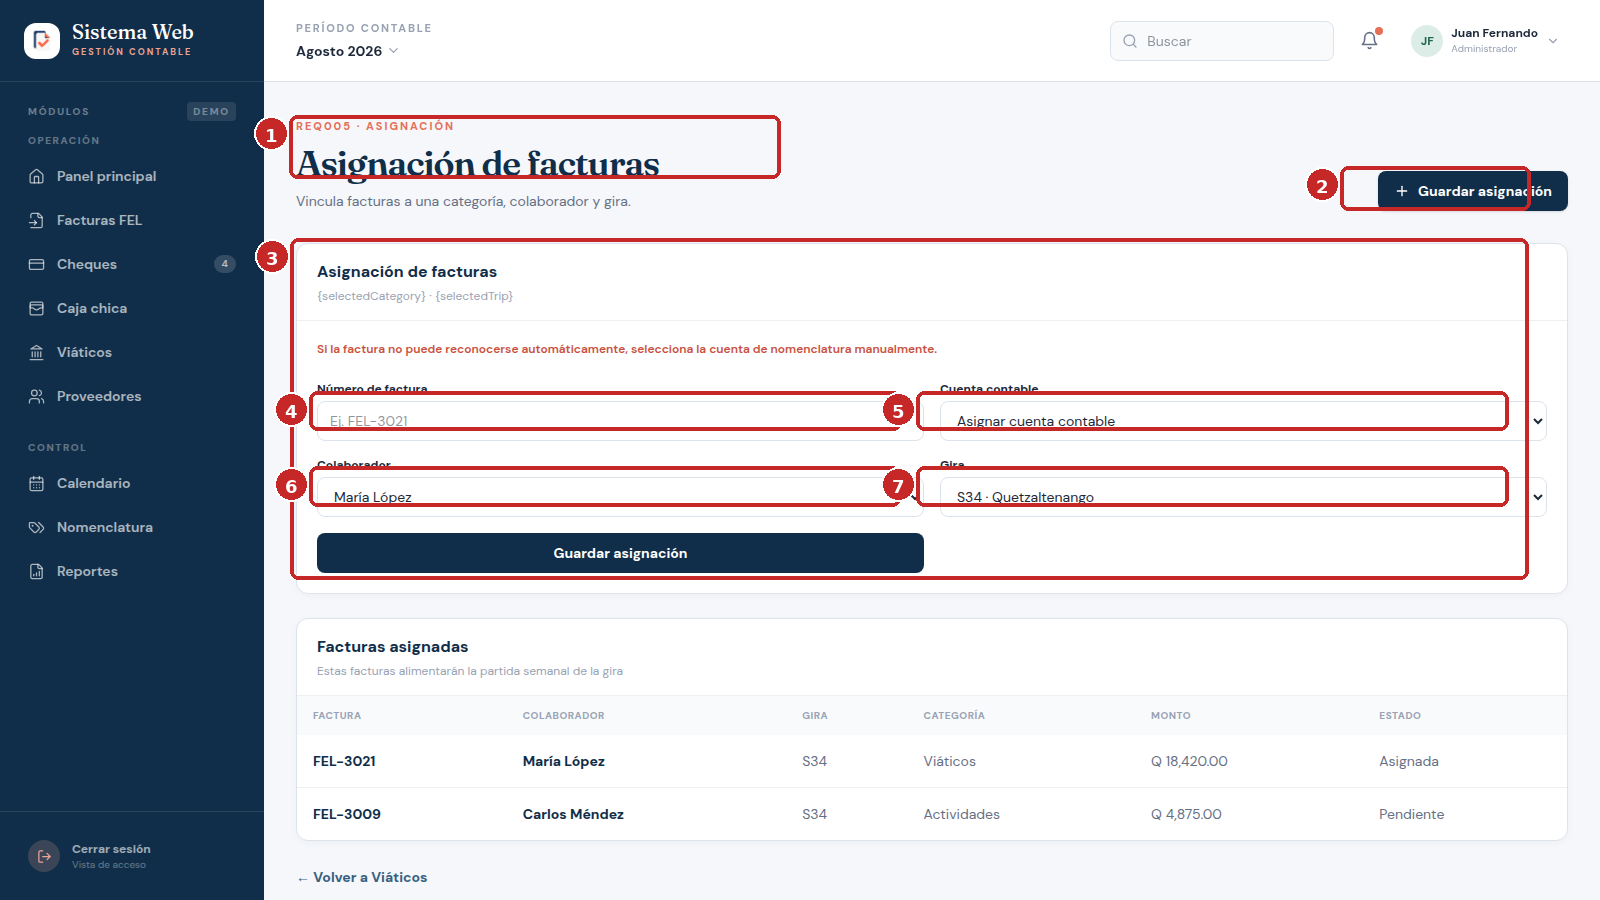
\includegraphics[width=0.92\linewidth]{capturas_reales/anotadas/pantalla_07_asignacion_facturas_anotada.png}
    \caption*{Nota. Elaboración propia a partir del prototipo funcional.}
\end{figure}

\begin{enumerate}
\item confirme la categoría y la gira seleccionadas.
\item escriba el número de factura.
\item seleccione la cuenta contable. Si el sistema no la reconoce, elija una cuenta registrada en Nomenclatura.
\item seleccione el colaborador.
\item seleccione la gira o territorio correspondiente.
\item presione ``Guardar asignación''.
\item confirme que la factura aparezca en la tabla de facturas asignadas con su estado correcto.
\end{enumerate}

\subsubsection{Proveedores}
Proveedores administra el registro por NIT, las condiciones de crédito, las retenciones, la cartera y las partidas.

\begin{figure}[H]
    \centering
    \caption{Módulo de Proveedores con anotaciones numeradas.}
    \label{fig:manual_usuario_pantalla_08_proveedores_anotada}
    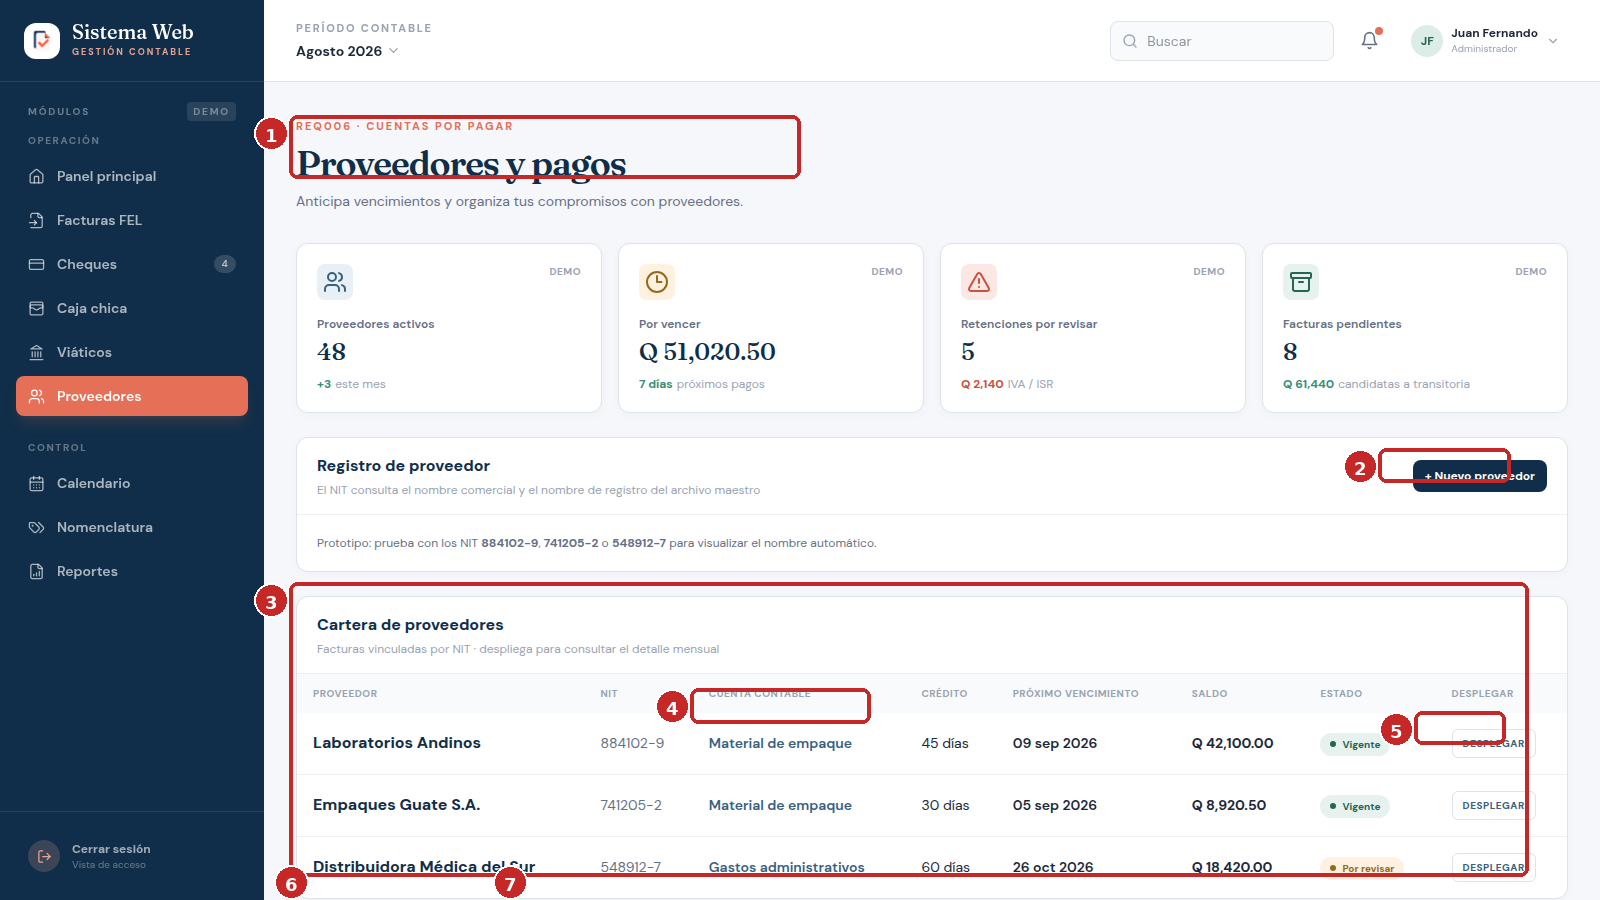
\includegraphics[width=0.92\linewidth]{capturas_reales/anotadas/pantalla_08_proveedores_anotada.png}
    \caption*{Nota. Elaboración propia a partir del prototipo funcional.}
\end{figure}

\begin{enumerate}
\item presione ``Nuevo proveedor'' para iniciar el registro.
\item escriba el NIT. El sistema consultará el nombre comercial y el nombre de registro disponibles.
\item revise la cartera con proveedor, NIT, cuenta contable, crédito, vencimiento, saldo y estado.
\item confirme la cuenta de Nomenclatura asociada al proveedor.
\item presione ``Desplegar'' para consultar las facturas mensuales.
\item presione ``Generar partida dentro del mes'' para obligaciones pagaderas en el período.
\item presione ``Generar partida transitoria'' para facturas pendientes de pago.
\end{enumerate}

\subsubsection{Calendario operativo}
Calendario presenta depósitos, pagos, cheques, giras y otras actividades por período.

\begin{figure}[H]
    \centering
    \caption{Módulo de Calendario con anotaciones numeradas.}
    \label{fig:manual_usuario_pantalla_09_calendario_anotada}
    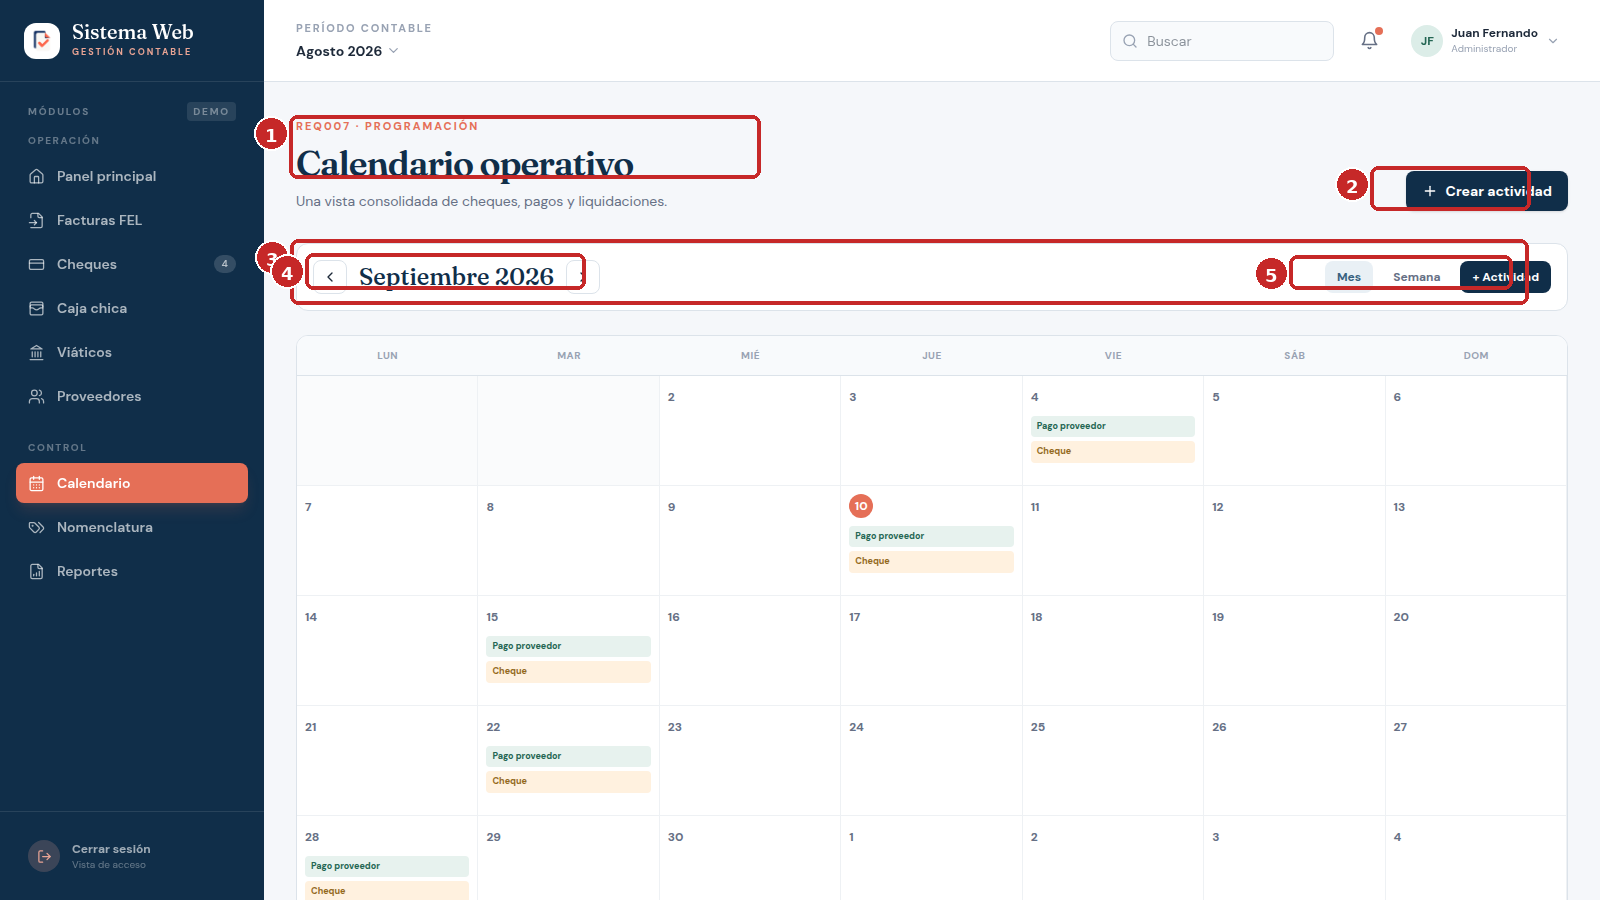
\includegraphics[width=0.92\linewidth]{capturas_reales/anotadas/pantalla_09_calendario_anotada.png}
    \caption*{Nota. Elaboración propia a partir del prototipo funcional.}
\end{figure}

\begin{enumerate}
\item revise el mes y año mostrados.
\item utilice las flechas para cambiar de período.
\item presione ``Mes'' para conservar la vista mensual.
\item consulte los eventos ubicados en cada fecha, como ``Pago proveedor'' y ``Cheque''.
\item presione ``Actividad'' para registrar una nueva actividad cuando tenga autorización.
\end{enumerate}

\subsubsection{Nomenclatura contable}
Nomenclatura contiene las cuentas que alimentan las sugerencias y partidas del sistema.

\begin{figure}[H]
    \centering
    \caption{Módulo de Nomenclatura con anotaciones numeradas.}
    \label{fig:manual_usuario_pantalla_10_nomenclatura_anotada}
    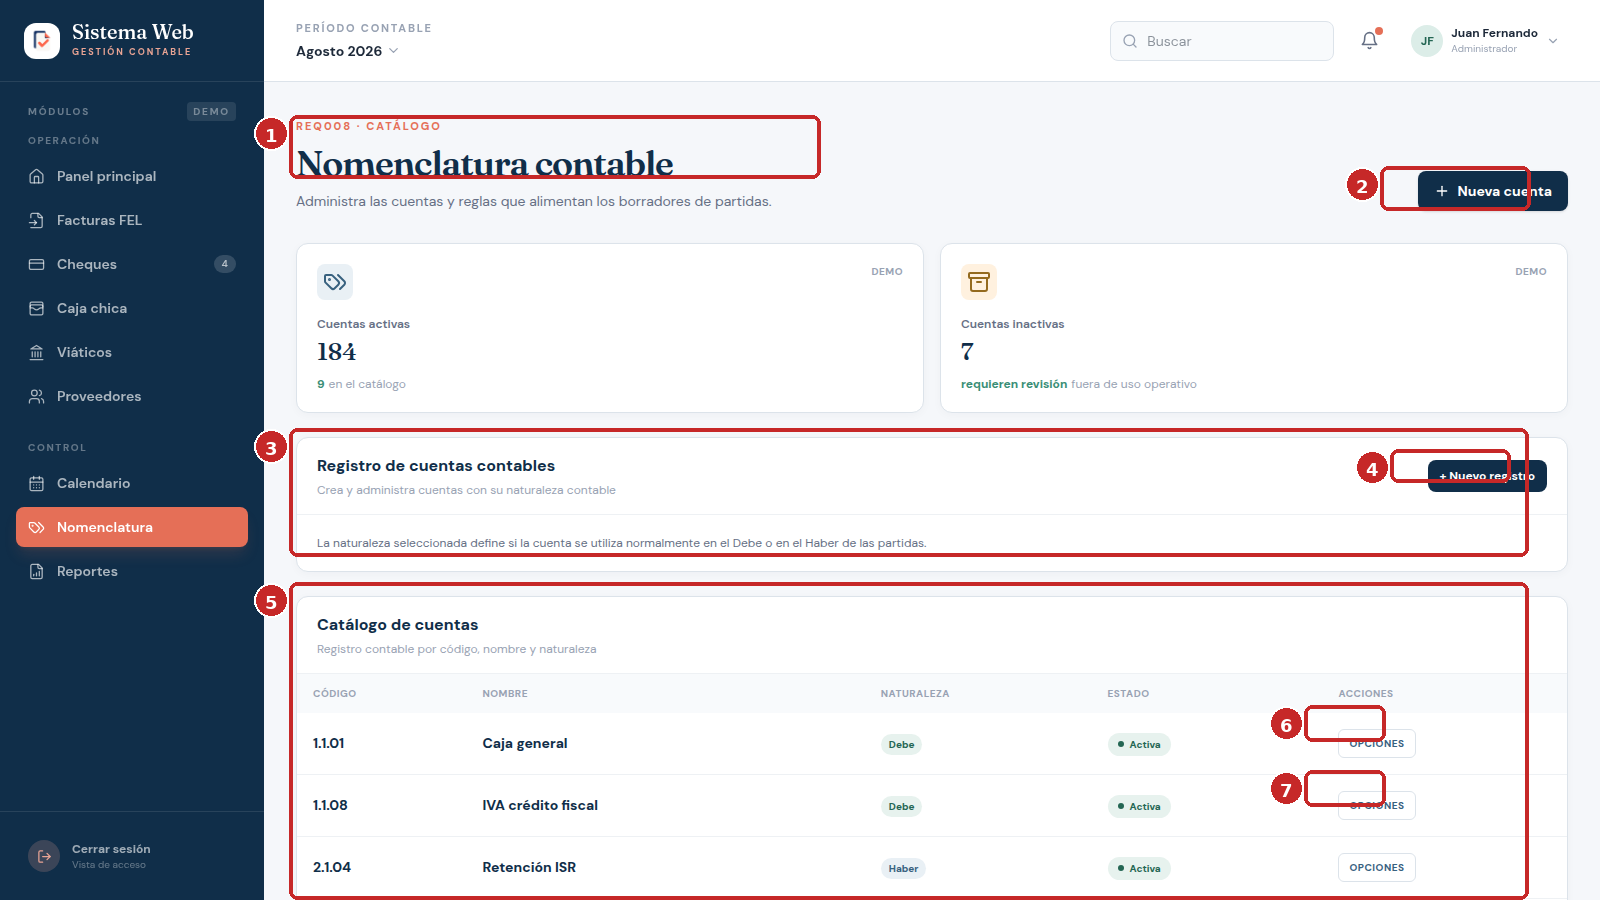
\includegraphics[width=0.92\linewidth]{capturas_reales/anotadas/pantalla_10_nomenclatura_anotada.png}
    \caption*{Nota. Elaboración propia a partir del prototipo funcional.}
\end{figure}

\begin{enumerate}
\item presione ``Nueva cuenta'' cuando corresponda crear una cuenta.
\item presione ``Nuevo registro'' para abrir el formulario de cuenta.
\item escriba código y nombre y seleccione la naturaleza Debe o Haber.
\item guarde el registro y verifique que la cuenta aparezca en el catálogo.
\item consulte el código, nombre, naturaleza y estado de cada cuenta.
\item abra ``Opciones'' para administrar el registro según sus permisos.
\end{enumerate}

\subsubsection{Reportes}
Reportes permite seleccionar el tipo de información, el período y los filtros para obtener indicadores.

\begin{figure}[H]
    \centering
    \caption{Módulo de Reportes con anotaciones numeradas.}
    \label{fig:manual_usuario_pantalla_11_reportes_anotada}
    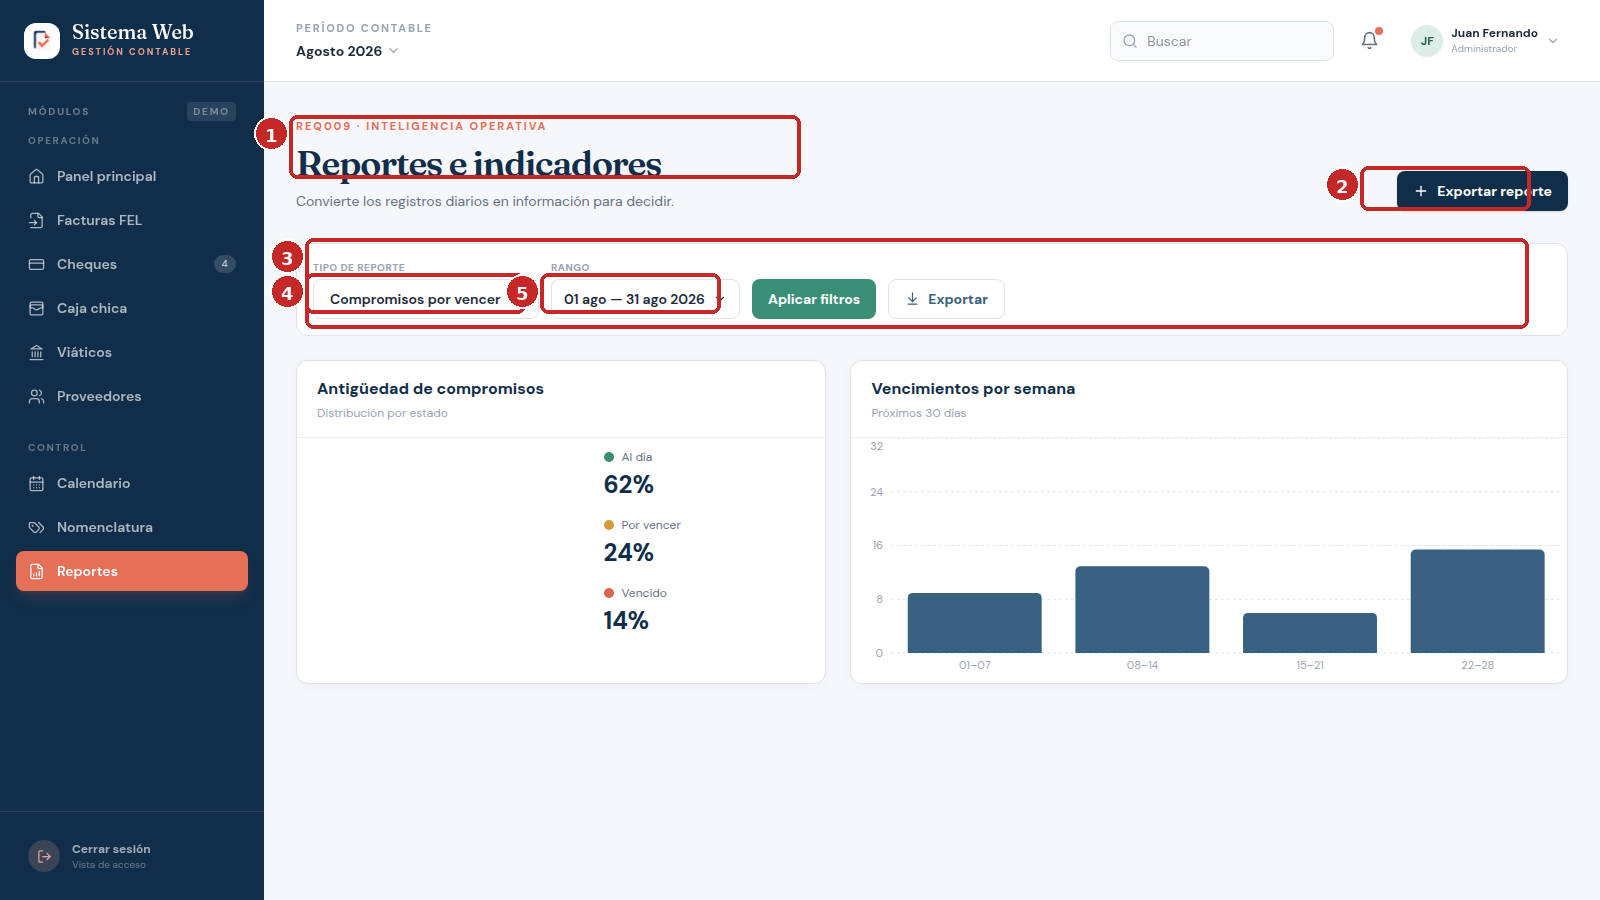
\includegraphics[width=0.92\linewidth]{capturas_reales/anotadas/pantalla_11_reportes_anotada.png}
    \caption*{Nota. Elaboración propia a partir del prototipo funcional.}
\end{figure}

\begin{enumerate}
\item confirme que se encuentra en ``Reportes e indicadores''.
\item seleccione el tipo de reporte.
\item seleccione el rango de fechas.
\item presione ``Aplicar filtros''.
\item presione ``Exportar'' para descargar o preparar el reporte autorizado.
\end{enumerate}

\subsubsection{Resumen de Caja chica}
El resumen presenta los movimientos que se imprimirán o archivarán.

\begin{figure}[H]
    \centering
    \caption{Resumen de Caja chica con anotaciones numeradas.}
    \label{fig:manual_usuario_pantalla_12_resumen_caja_anotada}
    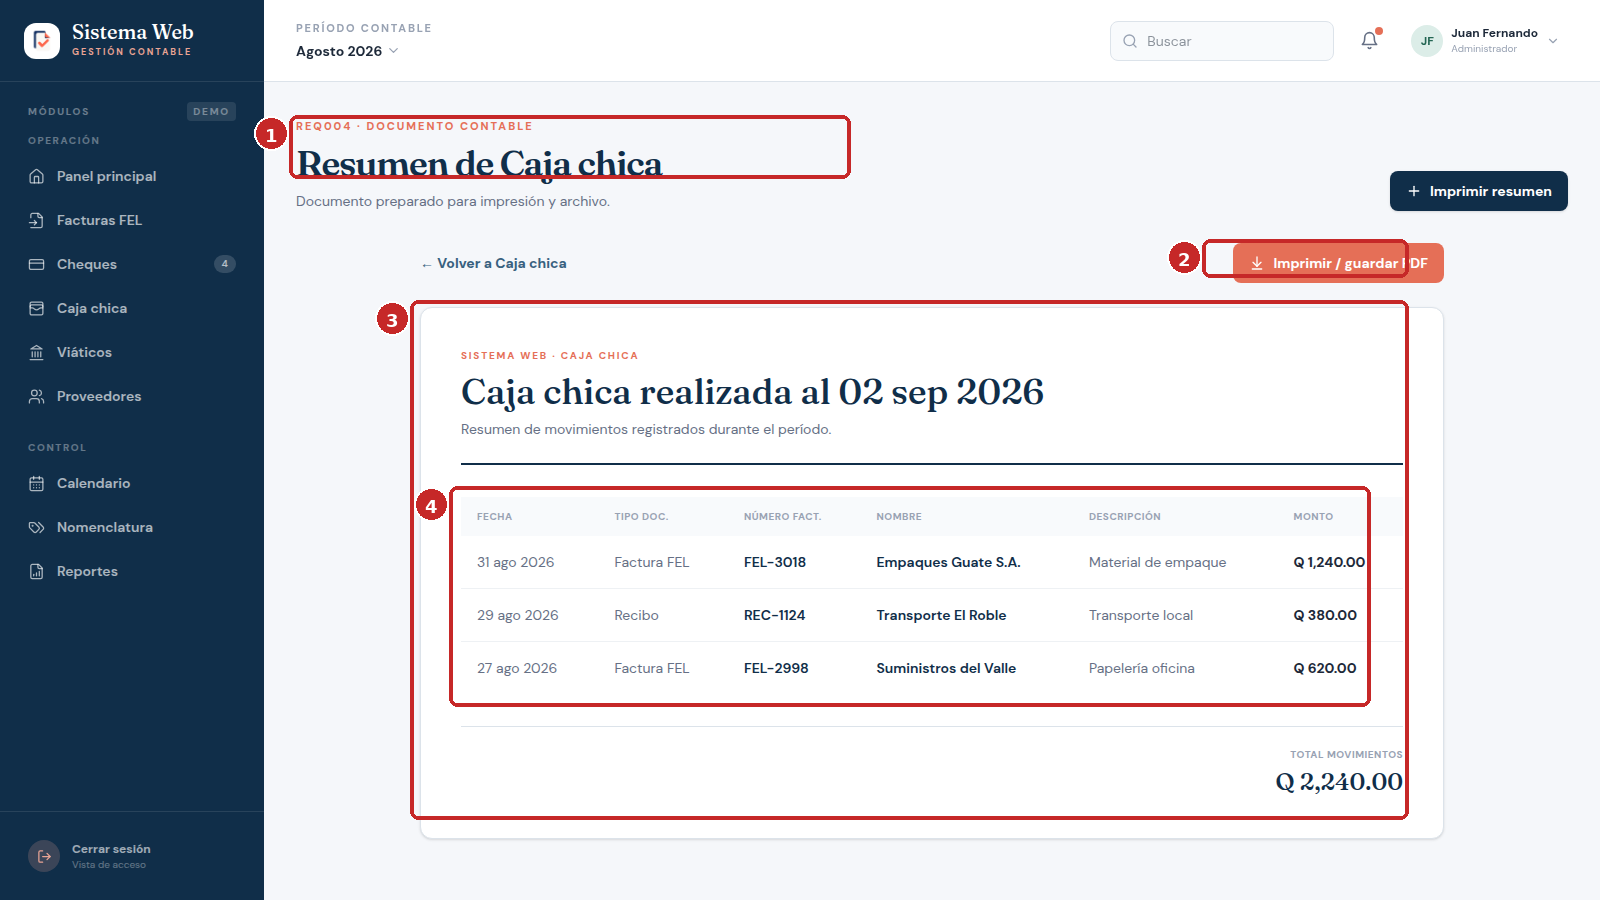
\includegraphics[width=0.92\linewidth]{capturas_reales/anotadas/pantalla_12_resumen_caja_anotada.png}
    \caption*{Nota. Elaboración propia a partir del prototipo funcional.}
\end{figure}

\begin{enumerate}
\item confirme el título y la fecha del resumen.
\item presione ``Imprimir / guardar PDF''.
\item verifique que el documento incluya fecha, tipo de documento, número, nombre, descripción y monto.
\item revise el total de movimientos antes de imprimir o guardar el archivo.
\end{enumerate}

\subsubsection{Mensajes de error y solución}
Cuando las credenciales sean rechazadas, vuelva a escribir el usuario y la contraseña. Si una factura no puede clasificarse, asígnele manualmente una cuenta de Nomenclatura. Si falta un dato obligatorio, complete el campo señalado antes de guardar. Si una partida no cuadra, revise Debe, Haber, IVA, retenciones y descuentos. Si la pantalla no carga, actualice el navegador y comuníquese con soporte si el problema persiste.

\subsubsection{Recomendaciones de seguridad}
Mantenga sus credenciales bajo resguardo, cierre sesión al terminar, revise los documentos antes de aprobarlos y no elimine información sin autorización. Verifique siempre que la cuenta contable corresponda al gasto y que la operación se registre en el período correcto.

\subsubsection{Flujo recomendado de trabajo}
Para mantener la trazabilidad contable, inicie el período revisando el Panel principal, importe las facturas FEL/SAT, verifique los cheques y registre las operaciones de Caja chica. Posteriormente, asigne las facturas de viáticos, actualice la cartera de proveedores, revise el Calendario y genere los reportes autorizados.

\subsubsection{Cierre de operaciones}
Antes de cerrar el período, confirme que las facturas tengan una cuenta de Nomenclatura, que las partidas estén cuadradas, que los cheques tengan el estado correcto y que las facturas pendientes se encuentren identificadas como partidas transitorias. Guarde los reportes autorizados según las políticas internas.

\subsubsection{Glosario básico}
\begin{description}
\item[FEL/SAT] Factura electrónica y documentos tributarios consultados o importados desde la información del SAT.
\item[Nomenclatura] Catálogo de cuentas contables utilizado para clasificar gastos y construir partidas.
\item[Partida transitoria] Registro contable temporal utilizado cuando una factura está pendiente de pago.
\item[Viático] Gasto asociado a una gira, colaborador, territorio y semana de trabajo.
\item[Arqueo o resumen] Documento de revisión de movimientos y saldo de Caja chica.
\end{description}

\subsubsection{Seguimiento y trazabilidad de operaciones}
Cada registro debe revisarse antes de continuar con el siguiente paso. Cuando una operación genere una partida, una asignación o un cambio de estado, conserve el número de documento, la fecha y el módulo en el que se realizó. Esta información facilita la revisión posterior y permite comunicar una incidencia con datos verificables.

\subsubsection{Criterios de revisión antes del cierre}
Antes de finalizar la jornada o el período, confirme que las operaciones guardadas correspondan al período correcto, que no existan documentos duplicados y que las cuentas contables utilizadas estén activas. Cuando el sistema solicite una asignación manual, seleccione la cuenta que corresponda al gasto y solicite una segunda revisión si la operación afecta una partida contable.

\subsubsection{Atención de incidencias}
Cuando una operación no produzca el resultado esperado, registre la fecha, el módulo, la acción realizada y el mensaje mostrado. Evite repetir una importación o un registro hasta confirmar que la primera operación no fue guardada. El reporte debe remitirse al responsable designado sin incluir contraseñas, tokens ni información que no sea necesaria para diagnosticar el problema.


\end{document}